\documentclass[11pt]{report}
\usepackage[utf8]{inputenc}
\usepackage{formatting}
\usepackage{mathpazo}
\usepackage[nottoc,numbib]{tocbibind}
\usepackage{etoolbox}
\usepackage[all]{nowidow} % prevent single lines by themselves
\usepackage{lipsum}
\usepackage{tabto}

\usepackage[color=]{siunitx}
\sisetup{per-mode=power}
\DeclareSIUnit\molar{\mole\per\cubic\deci\metre}


\title{On the neurophysiology underlying broadband electric field fluctuations at the scalp}
\author{Niklas Brake}
\date{\today}
% \setcounter{secnumdepth}{0} % to remove numbers

\fancypagestyle{plain}{%redefining plain pagestyle
\renewcommand{\headrulewidth}{0pt}
\fancyhf{} %clear all headers and footers fields
\fancyfoot[C]{\color{seccolor}\thepage} %prints the page number on the right side of the header
}

\begin{document}

\thesistitle
\onehalfspacing

\fancyfoot[R]{\color{seccolor}\thepage}
\fancyhead[L]{{\color{gray}\nouppercase{Table of contents}}}
\renewcommand{\cftchapfont}{\scshape\bfseries}
\renewcommand{\cftchappagefont}{\bfseries}
\renewcommand{\cftsubsecfont}{\small}
\pagenumbering{roman}

\newpage

\setlength{\parskip}{6pt}
\setlength{\skip\footins}{18pt}
\setlength{\footnotesep}{\baselineskip}

%%%%%%%%%%%%%%%%%%%%%%%%%%%%%%%%%%%%%%%%%%%%%%%%%%
\chapter*{Abstract}
\addcontentsline{toc}{chapter}{Abstract}
\fancyhead[L]{{\color{gray}\nouppercase{Abstract}}}
Electrophysiological measurements of neural tissue allow us to observe millisecond changes in neural activity, across a broad range of spatial scales from micrometers to centimeters. At these larger spatial scales, electrophysiological measurements can be made entirely noninvasively through the recording of electrical potentials at the scalp, known as electroencephalography (EEG). Periodic oscillations in these signals are known to reflect rhythmic brain activity, whereas broadband fluctuations remain poorly understood in comparison. Broadband fluctuations are evident from the continuous background trend in EEG spectra on top of which the peaks corresponding to brain rhythms are superimposed. Interpretations of this spectral trend range from irrelevant noise, to an epiphenomenon of brain rhythms, to a reflection of aperiodic brain activity. This lack of consensus sustains several open questions in the field. How should differences in the spectral trend be interpreted? Does this trend contaminate brain rhythm measurements? If so, how should spectra be rectified? In this thesis, I address these questions through the development of biophysical and statistical models of EEG generation that integrate both emerging physiological details as well as new experimental observations. The thesis comprises two manuscripts. The first manuscript concludes that spectra are predominantly shaped by the gating kinetics of γ-aminobutyric acid type A receptors. These kinetics produce a prominent Lorentzian shape in EEG spectra below approximately \qty{60}{\hertz} that is independent of neural dynamics. Consequently, systemic changes in synaptic currents perturb brain rhythm estimates unless spectra are rectified by fitting and correcting this Lorentzian trend. Furthermore, EEG can reflect aperiodic synaptic activity and therefore identifying spectral peaks is a critical precondition for measuring differences in brain rhythms. The second manuscript concludes that the spectral trend above \qty{60}{\hertz} is partially due to the gating kinetics of fast glutamate receptors and mostly due to noise. Oscillatory spiking activity can produce EEG signals between approximately 60 and 600, but unlike at lower frequencies defining the power of these high frequency oscillations relative to the spectral trend is unjustified. In sum, this thesis presents a theory of the physiological mechanisms underlying broadband EEG signals and outlines practical implications for the analysis and interpretation of EEG data.

\newpage

\chapter*{Résumé}
\addcontentsline{toc}{chapter}{Résumé}
\fancyhead[L]{{\color{gray}\nouppercase{Résumé}}}
Les mesures électrophysiologiques des tissus neuronaux nous permettent d'observer les changements de l'activité neuronale à la milliseconde, sur une large gamme d'échelles spatiales allant du micromètre au centimètre. À ces échelles spatiales plus grandes, les mesures électrophysiologiques peuvent être effectuées de manière entièrement non invasive grâce à l'enregistrement de potentiels électriques au niveau du cuir chevelu, connu sous le nom d'électroencéphalographie (EEG). Les oscillations périodiques de l'EEG sont observées et caractérisées depuis longtemps, alors que la nature des fluctuations à large bande de ces signaux reste mal comprise en comparaison. Les fluctuations à large bande sont évidentes en raison de la tendance de fond continue des spectres EEG, sur laquelle se superposent les pics correspondant aux rythmes cérébraux. Les interprétations de cette tendance spectrale vont d'un bruit non pertinent à un épiphénomène des rythmes cérébraux, en passant par le reflet d'un régime apériodique de l'activité neuronale. Cette absence de consensus entretient plusieurs questions ouvertes dans ce domaine. Comment interpréter les différences de tendance spectrale? Cette tendance contamine-t-elle les mesures du rythme cérébral? Dans cette thèse, j'aborde ces questions en développant des modèles biophysiques et statistiques de la génération d'EEG qui intègrent à la fois des détails physiologiques émergents et de nouvelles observations expérimentales. La thèse comprend deux manuscrits. Le premier manuscrit conclut que l'EEG n'est pas seulement une mesure des rythmes cérébraux, mais qu'il peut aussi refléter l'activité synaptique apériodique. De plus, à des fréquences inférieures à environ 60 Hz, les spectres sont fortement modelés par la cinétique de gating des récepteurs de classe A de l'acide γ-aminobutyrique. Cette cinétique produit une forme lorentzienne proéminente dans les spectres EEG, qui est indépendante de la dynamique neuronale. Par conséquent, les changements systémiques dans les courants synaptiques perturbent les estimations du rythme cérébral, à moins que les spectres ne soient rectifiés en ajustant et en corrigeant la tendance lorentzienne. Le second manuscrit conclut que l'activité dopante ne peut pas générer de signaux EEG à large bande, mais qu'elle peut générer des oscillations à haute fréquence entre 60 et 600 Hz environ. Ces conclusions suggèrent qu'il est inutile de mesurer les oscillations à haute fréquence par rapport à la tendance spectrale, contrairement à ce qui se passe pour les rythmes cérébraux à basse fréquence. En résumé, cette thèse présente une théorie des mécanismes physiologiques sous-jacents aux signaux EEG à large bande et souligne les implications pratiques pour l'analyse et l'interprétation des données EEG.

%%%%%%%%%%%%%%%%%%%%%%%%%%%%%%%%%%%%%%%%%%%%%%%%%%
\newpage
\chapter*{Acknowledgements}
\addcontentsline{toc}{chapter}{Acknowledgements}
\fancyhead[L]{{\color{gray}\nouppercase{Acknowledgements}}}



%%%%%%%%%%%%%%%%%%%%%%%%%%%%%%%%%%%%%%%%%%%%%%%%%%
\newpage
\chapter*{Contribution of authors}
\addcontentsline{toc}{chapter}{Contribution of authors}
\fancyhead[L]{{\color{gray}\nouppercase{Contribution of authors}}}

\setlength{\parindent}{0pt}
\setlength{\parskip}{3pt}

This thesis is presented as a manuscript-based thesis. I describe below the individual contributions to each manuscript that together constitute the main chapters of my thesis using the CRediT taxonomy. The final manuscript is included as an appendix as it does not directly relate to the main focus of my thesis.

\vspace{.5em} 
Chapter 2 \hrule

\hangindent=1cm Brake N, Duc F, Rokos A, Arseneau F, Shahiri S, Khadra A, and Plourde G. A neurophysiological basis for aperiodic EEG and the background spectral trend. \textit{Nature Communications} \textbf{15}, 1514 (2024). \url{https://doi.org/10.1038/s41467-024-45922-8}

{\small \textbf{Brake N}: Conceptualization, Data curation, Formal analysis, Investigation, Methodology, Software, Visualization, Writing—original draft, Writing—review and editing. \textbf{Duc F}: Investigation. \textbf{Rokos A}: Investigation. \textbf{Areseau F}: Investigation. \textbf{Shahiri S}: Investigation. \textbf{Khadra A}: Conceptualization, Funding acquisition, Project administration, Supervision, Writing—review and editing. \textbf{Plourde G}: Conceptualization, Data curation, Funding acquisition, Investigation, Project administration, Supervision, Writing—review and editing.}

\vspace{.5em} Chapter 3 \hrule

\hangindent=1cm Brake N and Khadra A. Contributions of action potentials to scalp EEG: theory and biophysical simulations. \textit{eLife}. Available from: \url{https://doi.org/10.1101/2024.05.28.596262}

{\small \textbf{Brake N}: Conceptualization, Methodology, Investigation, Writing- Original draft preparation, Visualization. \textbf{Khadra A}: Supervision, Funding Acquisition, Writing- Reviewing and Editing.}

\vspace{.5em} 

Appendix A \hrule

\hangindent=1cm Brake N*, Mancino AS*, Yan Y, Shimomura T, Kubo Y, Khadra A, and Bowie D. Closed-state inactivation of cardiac, skeletal, and neuronal sodium channels is isoform specific. \textit{Journal of General Physiology} \textbf{154}, 7: e202112921 (2022). \url{https://doi.org/10.1085/jgp.202112921}

{\small \textbf{Brake N}: Conceptualization, Methodology, Formal Analysis, Investigation, Writing—Original Draft, Visualization.  \textbf{Mancino AS}: Conceptualization, Formal Analysis, Investigation. \textbf{Yan Y}: Formal analysis, Investigation. \textbf{Shimomura T}: Methodology, Formal analysis. \textbf{Kubo Y}: Methodology, Funding acquisition. \textbf{Khadra A}: Funding Acquisition, Supervision. \textbf{Bowie D}: Conceptualization, Funding Acquisition, Writing—Original Draft, Supervision, Project Administration.}

\setlength{\parskip}{6pt}
\setlength{\parindent}{17pt}

%%%%%%%%%%%%%%%%%%%%%%%%%%%%%%%%%%%%%%%%%%%%%%%%%%
\newpage
\chapter*{Contribution to original knowledge}
\addcontentsline{toc}{chapter}{Contribution to original knowledge}
\fancyhead[L]{{\color{gray}\nouppercase{Contribution to original knowledge}}}
\renewcommand{\chapterautorefname}{Chapter}

Despite a century of EEG recordings under our belt, the question ``what does EEG actually represent about the brain?'' has yet to be completely answered. In recent years, the overall background spectral trend observed in EEG signals has received particular interest and has been extensively characterized. Yet, the origin and interpretation of this EEG feature remains intensely debated. The major theories on the EEG spectral trend rely principally on conceptual and phenomenological modelling. Broadly speaking, this thesis contributes to our understanding of the neural basis of EEG by providing a comprehensive biophysical theory of how the EEG spectral trend can be generated by neural activity. This theory is built from several novel findings:

Firstly, scientist had argued conceptually whether EEG signals can reflect asynchronous background neural activity. This thesis presents biophysical calculations that show it is impossible for asynchronous neural activity to be detected on an EEG, providing the first argument against this interpretation that combines both biophysical EEG simulations and experimentally determined physiological parameters of neural activity (\autoref{sec:natcomms}). 

Secondly, it was not known whether EEG signals can reflect non-oscillatory neural activity. This thesis presents the results of numerical simulations which demonstrate that aperiodic activity of a similar nature to that observed experimentally in animals can produce detectable EEG signals, providing the first evidence that EEG signals can theoretically reflect aperiodic neural activity (\autoref{sec:natcomms}).

Thirdly, it is debated how the EEG spectral trend should be corrected for when quantifying brain rhythms. This thesis examines the spectral changes known to be caused by the administration of the drug propofol, a general anesthetic. The results illustrate how broadband changes in EEG spectra arise from propofol's known pharmacology using biophysical models of electric field generation. These simulations demonstrate how the changes induced by propofol at the single cell level alter the production of rhythmic EEG signals, and provide the first concrete, biophysically justified case where changes in the EEG spectra trend corrupt brain rhythms estimates (\autoref{sec:natcomms}).

Fourthly, the thesis proposes how the effects of propofol on the EEG spectral trend should be rectified. Quantitatively accounting for these changes on EEG collected from patients undergoing propofol anesthesia revealed for the first time that loss of consciousness from propofol is time locked exclusively to delta rhythms, in contrast to past studies that have implicated both alpha and delta rhythms  (\autoref{sec:natcomms}).

Finally, it was not known whether or not action potentials can generate detectable EEG signals. Dissenting opinions were based on conceptual arguments, while concurring opinions were based on extrapolation from local field recordings. This thesis details the results of biophysical simulations and EEG forward modelling, which demonstrate that action potentials cannot generate aperiodic EEG signals (\autoref{sec:apEEG}). These simulations also, for the first time, define a frequency range where EEG rhythms can reasonably be generated by action potentials (\autoref{sec:apEEG}).

In addition to the main chapters of the thesis, I also include an appendix which details work done during my PhD that is not directly related to the neural basis of EEG. This work produced original knowledge about the molecular basis of voltage sensing in proteins called voltage-gated sodium channel. This work showed for the first time that the molecular domains of the sodium channel protein have different functions depending on the protein isoform. Specifically, most investigations had been performed on the sodium channel expressed by skeletal muscle, which had concluded that the fourth voltage sensing domain is alone responsible for channel inactivation. The results presented in \autoref{sec:Nav} illustrate that in the cardiac sodium channel, both the third and fourth domains are necessary for channel inactivation. Additionally, the work details how closed-state inactivation is variable among sodium channel isoforms. Experimental evidence from the skeletal muscle channel indicated that the fourth voltage sensing domain moves extremely slowly in response to changes in the electric field relative to the other three domains, which would prevent closed state inactivation. We show that the cardiac sodium channel has a very high propensity for closed state inactivation, indicating that the dynamics of the various voltage sensing domains must differ among channel isoforms (\autoref{sec:Nav}).



%%%%%%%%%%%%%%%%%%%%%%%%%%%%%%%%%%%%%%%%%%%%%%%%%%
% \newpage
% \chapter*{List of figures}
\addcontentsline{toc}{chapter}{List of figures}
\fancyhead[L]{{\color{gray}\nouppercase{List of figures}}}
 
\renewcommand{\cftfigpresnum}{\bfseries \color{seccolor}\figurename\ }
\settowidth{\cftfignumwidth}{Figure 00.0000}
\renewcommand\cftfigindent{0pt}  % no indentation

% Get rid of header for list of figures
\makeatletter
\renewcommand\listoffigures{%
        \@starttoc{lof}%
}
\makeatother

% Get rid of header for list of tables
\makeatletter
\renewcommand\listoftables{%
        \@starttoc{lot}%
}
\makeatother

\setlength{\parskip}{0pt}

\listoffigures

\newpage
\chapter*{List of tables}
\addcontentsline{toc}{chapter}{List of tables}
\fancyhead[L]{{\color{gray}\nouppercase{List of tables}}}

\renewcommand{\cfttabpresnum}{\bfseries \color{seccolor}\tablename\ }
\settowidth{\cfttabnumwidth}{Table 00.0000}
\renewcommand\cfttabindent{0pt}  % no indentation
\listoftables

\setlength{\parskip}{6pt}

%%%%%%%%%%%%%%%%%%%%%%%%%%%%%%%%%%%%%%%%%%%%%%%%%%
% \newpage
% \chapter*{List of abbreviations}
\addcontentsline{toc}{chapter}{List of abbreviations}
\fancyhead[L]{{\color{gray}\nouppercase{List of abbreviations}}}

\setlength{\parindent}{0pt}
\setlength{\parskip}{3pt}
\secbfcolor{AIDS} \tabto{5.5em} Acquired immunodeficiency syndrome

\secbfcolor{AIH} \tabto{5.5em} Autoimmune hepatitis

\secbfcolor{AIRE} \tabto{5.5em} Autoimmune regulator

\secbfcolor{APC} \tabto{5.5em} Antigen presenting cell

\secbfcolor{Arm} \tabto{5.5em} Armstrong

\secbfcolor{BCR} \tabto{5.5em} B cell receptor

\secbfcolor{BM} \tabto{5.5em} Bone marrow

\secbfcolor{CD} \tabto{5.5em} Cluster of differentiation

\secbfcolor{CFU} \tabto{5.5em} Colony forming unit

\secbfcolor{Cl13} \tabto{5.5em} Clone 13

\secbfcolor{CNS} \tabto{5.5em} Central nervous system

% \secbfcolor{cTEC} \tabto{5.5em} Cortical thymic epithelial cell

\secbfcolor{CTL} \tabto{5.5em} Cytotoxic T lymphocyte

\secbfcolor{CTLA} \tabto{5.5em} Cytotoxic T lymphocyte-associated protein

\secbfcolor{DAMP} \tabto{5.5em} Damage-associated molecular pattern

\secbfcolor{DNA} \tabto{5.5em} Deoxyribonucleic acid 

\secbfcolor{EAE} \tabto{5.5em} Experimental autoimmune encephalomyelitis

\secbfcolor{FOXP} \tabto{5.5em} Forkhead box protein

\secbfcolor{GP} \tabto{5.5em} Glycoprotein

\secbfcolor{HA} \tabto{5.5em} Hemagglutinin

\secbfcolor{HCV} \tabto{5.5em} Hepatitis C virus

\secbfcolor{HIV} \tabto{5.5em} Human immunodeficiency virus

\secbfcolor{IAV} \tabto{5.5em} Influenza A virus

\secbfcolor{IFN} \tabto{5.5em} Interferon

\secbfcolor{IGRP} \tabto{5.5em} Islet-specific glucose-6-phosphatase-related protein

\secbfcolor{IL} \tabto{5.5em} Interleukin

\secbfcolor{ITAM} \tabto{5.5em} Immunoreceptor tyrosine-based activated motifs

\secbfcolor{KO} \tabto{5.5em} Knockout

\secbfcolor{KPR} \tabto{5.5em} Kinetic proofreading

\secbfcolor{LAG} \tabto{5.5em} Lymphocyte activation gene

\secbfcolor{LCMV} \tabto{5.5em} Lymphocytic choriomeningitis virus

\secbfcolor{MFI} \tabto{5.5em} Mean fluorescence intensity

\secbfcolor{MHC} \tabto{5.5em} Major histocompatibility complex

\secbfcolor{MOG} \tabto{5.5em} Myelin oligodendrocyte glycoprotein

\secbfcolor{mRNA} \tabto{5.5em} Messenger ribonucleic acid

\secbfcolor{mTEC} \tabto{5.5em} Medullary thymic epithelial cell

\secbfcolor{NP} \tabto{5.5em} Nanoparticle

\secbfcolor{ODE} \tabto{5.5em} Ordinary differential equation

\secbfcolor{PBC} \tabto{5.5em} Primary biliary cholangitis

\secbfcolor{PDC} \tabto{5.5em} Pyruvate dehydrogenase complex

\secbfcolor{PFU} \tabto{5.5em} Plaque forming unit

\secbfcolor{pMHC} \tabto{5.5em} Peptide-major histocompatibility complex

\secbfcolor{qPCR} \tabto{5.5em} Quantitative polymerase chain reaction

\secbfcolor{RAG} \tabto{5.5em} Recombination-activating gene

\secbfcolor{RBC} \tabto{5.5em} Red blood cell

%\secbfcolor{RFI} \tabto{5.5em} Relative fluorescence intensity

\secbfcolor{RNA} \tabto{5.5em} Ribonucleic acid

\secbfcolor{SIV} \tabto{5.5em} Simian immunodeficiency virus

\secbfcolor{SPR} \tabto{5.5em} Surface plasmon resonance

\secbfcolor{TCR} \tabto{5.5em} T cell receptor

\secbfcolor{TdT} \tabto{5.5em} Terminal deoxynucleotidyl transferase

\secbfcolor{Tfh} \tabto{5.5em} T follicular helper

\secbfcolor{TGF} \tabto{5.5em} Transforming growth factor

\secbfcolor{Th} \tabto{5.5em} T helper

\secbfcolor{TRA} \tabto{5.5em} Tissue-restricted antigen

\secbfcolor{Tr1} \tabto{5.5em} T-regulatory type 1 cell

\secbfcolor{Treg} \tabto{5.5em} Regulatory T cell

\secbfcolor{WT} \tabto{5.5em} Wild-type

\setlength{\parindent}{16pt}
\setlength{\parskip}{6pt}

%%%%%%%%%%%%%%%%%%%%%%%%%%%%%%%%%%%%%%%%%%%%%%%%%%
\newpage

\renewcommand*\contentsname{\color{seccolor}Table of contents}
\titlecontents{section}[18pt]{\addvspace{3pt}}{\thecontentslabel\enspace}{}{\titlerule*[0.7064pc]{.}\contentspage}
\tableofcontents

\newpage

\renewcommand{\chaptermark}[1]{\markboth{#1}{#1}}
\fancyhead[R]{}
\fancyhead[L]{{\color{gray}\textit{\chaptername\ \thechapter}\ --\ \leftmark}}

\pagenumbering{arabic}
\setcounter{page}{1}

\renewcommand{\thefootnote}{\fnsymbol{footnote}}
\hypersetup{linkcolor=seccolor}

\chapter{Introduction and literature review} \label{sec:intro}


\section{General introduction}

The liminal space between biology and physics is perhaps nowhere more salient than in the study of electrophysiology, where the emergent properties that characterize life intersect with the fundamental laws of nature. This intersection is certainly most profound in the microscopic details of the brain where cognition and consciousness emerge from electric fields. Our ability to measure these electrical signals through unit and field recordings or by proxy through calcium imaging lets us dissect the physical implementations of animal behaviour. To the benefit of science and medicine, these electric fields can also be recorded non-invasively from humans using scalp electrodes.

Despite the coarseness of its measurements, the electroencephalogram (EEG) has proven itself to be highly useful. EEG studies of human subjects benefit from being able to associate brain signals with complex cognitive paradigms such as memory \cite{Osipova2006, Sauseng2009, Sauseng2010}, perception \cite{Rodriguez1999, Melloni2007,Fahrenfort2012}, and attention \cite{Hillyard1998, Makeig2002}, which are more difficult to perform and assess with animals. The ability to measure brain activity relatively cheaply and easily has also made EEG a fecund source of neuromarkers for neurological conditions and brain states, most notably epilepsy \cite{Engel1984,Noachtar2009} and sleep \cite{Wolpert1969, Prerau2016}. Its modern clinical applications have been extended to include monitoring depth of anesthesia \cite{Michael2008} and detecting brain ischemia \cite{Meghdadi2021}, while ongoing research is trying to use EEG to predict various neurological conditions, including autism \cite{Bosl2018}, dementia \cite{Meghdadi2021}, schizophrenia \cite{Meghdadi2021}, and depression \cite{DeAguiarNeto2019}. Outside the clinic, advances in wearable EEG technology has led to its growing commercial use in brain-machine interfaces \cite{Mahmood2021} and biofeedback technology \cite{Hunkin2021}. 

After a century of EEG recordings \cite{Berger1929}, a lot still remains unknown about what these signals actually reflect about the brain \cite{Cohen2017}, especially when compared to invasive measurements like single unit recordings. However, as the neurophysiological basis of EEG is elucidated, its valuable correlates to cognition, disease, and states of consciousness can be mapped onto its neural substrate and further interrogated in animal models --- this connection is an important translational axis for brain research \cite{da2013eeg}. A fair amount of success has come from investigating synchronous neural oscillations, which generate rhythms on the EEG and whose neural basis can be studied in both mice and monkeys \cite{Buzsaki2004}. Building on this work, recent studies have begun identifying and quantifying \textit{broadband} components of EEG signals and correlating these features, such as the slope of the power spectrum (\autoref{fig:phenomenology}A), with cognitive tasks \cite{Ouyang2020,Podvalny2015,He2010,Waschke2021}, age \cite{Voytek2015}, neurological disease \cite{Wang2022, Pertermann2019, Schaworonkow2021, OSTLUND2021100931, MOLINA2020562, Robertson2019, Roche2019}, and various states of consciousness \cite{Colombo2019, Stock2020, Lendner2020, MUTHUKUMARASWAMY2018582}. In contrast to the classically considered narrowband oscillations, however, broadband EEG features remain poorly defined and their neurophysiological basis is both undetermined and controversial. 

\begin{figure}[b!]
    \centering
    \includegraphics[width=\textwidth]{Figures/chapter1/spectral_trend.pdf}
    
    \caption{\textbf{Example spectra illustrating the broadband characteristics of EEG.} 
    (\textbf{A}) Average EEG power spectrum during eyes closed, showing a slope in log-log space of $-1.32$. Data re-plotted from Pritchard \cite{Pritchard1992}. (\textbf{B}) Spectrum of \qty{83}{\minute} electrocorticographic signal of awake subject from three different electrodes, collected by He et al.\cite{He2010}.  (\textbf{C}) Changes in EEG spectrum under various conditions reported by Colombo et al.\cite{Colombo2019}. Panel B is reprinted with minor formatting changes from Neuron, 66/3, Biyu J. He, John M. Zempel, Abraham Z. Snyder, Marcus E. Raichle, The Temporal Structures and Functional Significance of Scale-free Brain Activity, 353-369, Copyright (2010), with permission from Elsevier. Panel C is adapted with minor formatting changes from Colombo et al. \cite{Colombo2019} under a Creative Commons license. © 2019 Colombo et al (CC BY-NC-ND 4.0).
    } 
    \label{fig:phenomenology}
\end{figure}

\section{Broadband EEG features and the spectral trend} \label{sec:phenomenon}
\subsection{Early characterization of broadband EEG}
Despite the relatively recent interest in broadband EEG, the fact that EEG signals exhibit broadband characteristics was noted in 1938 in the very first publication showing EEG spectra \cite{Grass1938}, which was computed with a mechanical apparatus of various wheels and projectors to transform the EEG output into Fourier space. If EEG signals were purely rhythmic, the spectrum should have shown discrete spectral peaks in narrow frequency bands corresponding to each of several possible rhythmic components. However, what the authors observed was a continuum of power across a broad range of frequencies, i.e., a broadband signal. Based on these spectra, the authors noted that ``inspection of such continuous spectrums should convince one of the inadvisability of referring to certain potentials as alpha, beta, delta waves, etc.''\cite{Grass1938}. Inadvisable or not, this practice is still very much the norm today. After the introduction of computer analysis in the 1960s, EEG spectra became more routinely examined, but the broadband components of these spectra were only ever mentioned in passing \cite{Boudreau1963}. It was the prevailing view that the aim of EEG spectral analysis was the ``disclosure of sinusoidal periodicities buried in the random background activity'' \cite{Freeman1975}. 

In 1992, Pritchard \cite{Pritchard1992} published the first paper that considered the broadband properties of EEG signals as a feature in its own right. In his paper, Pritchard posited that EEG spectra exhibit power law scaling, i.e., $P\sim1/f^\beta$, with an exponent of $\beta=1.32$ (\autoref{fig:phenomenology}A) and used this to argue that the brain is fractal in nature~\footnote[2]{The spectral exponent is equivalent to the slope of the spectrum in log-log space. The phrase spectral exponent and spectral slope are therefore used interchangeably.}. This claim effectively kickstarted multiple competing theories on the origin and meaning of the background EEG spectrum (\autoref{sec:theories}). A later study by He et al. \cite{He2010} was the first to show explicitly that the spectral trend may disclose information about the brain and is not just noise to be ignored. Using a technique based on fractal theory, the authors separated out the rhythmic and $1/f$ fractal component of their signals, and showed that the spectral exponent changed with task performance \cite{He2010}. A plot of their data showing a spectrum from 0.01 to 100 \unit{\hertz} is shown in \autoref{fig:phenomenology}B and clearly illustrates how spectral peaks from brain rhythms seem to rise up out of a background spectral trend. A plot from a more recent paper \cite{Colombo2019} is shown in \autoref{fig:phenomenology}C to illustrate how the background spectral trend can change depending on brain state. 

To briefly summarize, the broadband component of EEG signals is characterized by the overall background trend observed in EEG spectra. From the original paper by Pritchard \cite{Pritchard1992}, estimating power laws from this trend has been of particular interest to the field, and changes in the spectral exponent have since been correlated with myriad behavioural and neurological variables.

\subsection{Relevance for studying brain rhythms} \label{sec:detrending}
Having a physiological explanation for the spectral trend is obviously important for interpreting results like those in \autoref{fig:phenomenology}C. Why is the slope of the spectrum changing? Additionally, a physiological interpretation of the spectral trend is important for studying the rhythmic component of EEG. Typically, the spectral trend is dealt with in one of several ways. By far the most common approach is to divide EEG spectra by the spectrum during a baseline condition. In cases that the spectral trend does not change, this technique removes the trend from the analysis. However, if the spectral trend changes between the conditions, e.g., \autoref{fig:phenomenology}C, this technique assumes that any change in a given frequency band is caused by differences in brain rhythms \cite{Gerster2022}.

Those who argue for a deeper meaning behind the spectral trend have developed EEG analyses that deal with the spectral trend explicitly. The first of these procedures is to ``whiten'' the spectrum by fitting and removing the spectral trend prior to analyzing changes in brain rhythms \cite{Buzsaki2004,Buzsaki2006,Donoghue2020}. A popular algorithm for fitting the spectral trend, called FOOOF \cite{Donoghue2020}, models the spectral peaks as Gaussian functions multiplied by a $1/f^\beta$ trend. In other words, this technique assumes that the spectral trend follows a power law and accounts for this power relationship when measuring brain rhythms. A less common technique is to recompute the EEG spectrum at different sampling frequencies. This is supposed to separate narrowband oscillations from any fractal component of the data, which due to the self-similar nature of fractals is invariant under temporal rescaling \cite{Yamamoto1993}. An algorithm based on this technique has been developed, called Irregular-Resampling Auto-Spectral Analysis (IRASA) \cite{Wen2016}. This analysis makes the specific assumption that the spectral trend reflects fractal brain activity and should be removed from brain rhythm estimates.

\begin{wrapfigure}[15]{r}{80mm}
\vspace{-15pt}
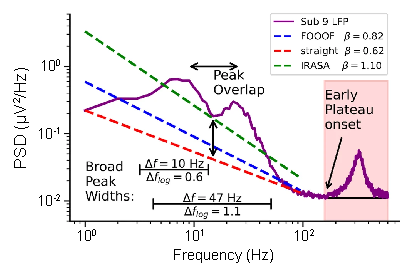
\includegraphics[width=75mm]{Figures/chapter1/gerster.pdf}
\vspace{-10pt}
\caption{ \captiontitle{Difficulties of estimating spectral exponents with various methods.} The spectrum of a macroscopic neural recording (purple), analyzed with three methods to estimate the spectral exponent, including FOOOF (blue line), IRASA (green line), and basic linear regression (red line). These methods give different values for $\beta$ (see legend). Above \qty{100}{\hertz}, the spectral trend plateaus. Figure modified from Gerster et al. \cite{Gerster2022} under a Creative Commons license. © 2022 Gerster et al (CC BY 4.0).
} \label{fig:gerster}
\end{wrapfigure}

These last two methods will lead to very different conclusions compared to a traditional baseline-normalized analysis. In fact, the last two methods produce different outcomes from \textit{each other} when applied to the same spectrum (\autoref{fig:gerster}). This inconsistency comes from lacking a unified, physiological definition of broadband EEG. Furthermore, at higher frequencies, spectra typically exhibit a plateau  (\autoref{fig:gerster}) whose origin and interpretation remain unresolved \cite{Gerster2022}. The techniques above do not provide a systematic approach to dealing with this part of the spectral trend other than restricting the frequency range of analysis. This limitation illustrates that, while prevalent, the power-law scaling description of EEG spectra does not capture the full broadband nature of EEG signals. 

In summary, every analysis procedure makes some assumption about the spectral trend which affects the interpretation of both the broadband and rhythmic components of EEG. Ignoring the trend makes the specific assumption that it should be included in brain rhythms estimates. Deciding to remove it requires a systematic quantification of the spectral trend and its interaction with brain rhythms. Currently, different studies use different methods for spectral analysis and may therefore interpret the same data in distinct ways. Moreover, many of the theories on the spectral trend do not yet have quantitative methods associated with them, and thus the methodologies described above only reflect a subset of the existing interpretations of broadband EEG --- all of which will be reviewed in detail later.

\subsection{Summary}
The past three decades have seen an increasing awareness that EEG exhibits broadband characteristics which change with task performance and brain state. This feature is most often described as a $1/f^\beta$ scaling of the EEG spectrum; analysis technique have been developed to estimate the spectral exponent, $\beta$, as well as to correct for the spectral trend when estimating brain rhythms. However, without a complete understanding of the mechanism(s) giving rise to the broadband characteristics of EEG, interpreting differences in the spectral trend has been speculative and the veracity of detrended EEG analyses has remained debatable. Understanding the neurophysiological basis of the EEG spectral trend is the central aim of this thesis, with the view that a comprehensive explanation of the spectral trend will improve interpretation and analysis of EEG data. In the main chapters, I will present biophysical modelling results that describe how neurophysiological systems might generate broadband EEG signals. In the remainder of this chapter, I provide background for the modelling work in this thesis with an overview of the biophysics and neural basis of EEG, before finally reviewing existing theories on the origin of the EEG spectral trend.

\section{The biophysics of EEG} \label{sec:EM_theory}

A strength of EEG, along with other electrophysiological measurements, is that the biophysics of these measurements are understood. In this section, I review the basics of electromagnetism in a volume conductor and build up to forward models of the EEG --- models that take a distribution of currents in the brain and give as an output the electric potential at the scalp.

\subsection{Maxwell's equations and the electric potential}
In 1873, James Clerk Maxwell published his treatise on electricity and magnetism, accomplishing for electromagnetism what Newton had for mechanics. In four equations, the behaviour of all classical phenomena related to electricity and magnetism could be described. As such, they are the basic laws that turn physiology into \textit{electro}physiology. The equations are
\begin{align*}
    & \nabla \cdot \bm{E} = \frac{\rho}{\epsilon_0}\mathrm{,} \\
    & \nabla \cdot \bm{B} = 0\mathrm{,} \\
    & \nabla \times \bm{E} = - \frac{\partial {B}}{\partial t}\mathrm{,} \\
    & \nabla \times \bm{B} = \mu \left( \bm{J} + \epsilon_0 \frac{\partial \bm{E}}{\partial t} \right)\mathrm{.}
\end{align*}
Here, $\bm{E}$ and $\bm{B}$ are vector fields called the electric and magnetic field, respectively. The first two equations describe the divergence of these fields and the latter two equations describe the curl of these fields. 

The first equation states that the sources (positive divergence) and sinks (negative divergence) of the electric field are electric monopoles, otherwise called an electric charge. $\rho$ is the density of charge at each point in space and when scaled by $\epsilon_0$, the permittivity of a vacuum, one gets the divergence of the electric field. Negative charges are sinks of the electric field and positive charges are sources of the electric field. The second equation states that there are no source or sinks of the magnetic field. In other words, there are no magnetic monopoles. The third and fourth equation describe how the electric and magnetic field interact with each other. The third equation is called Faraday's law of induction and describes how a time varying magnetic field can induce an electric field. The final equation is Ampère's law and describes how a magnetic field is generated by either an electric current or a time varying electric field.

\subsubsection{The quasi-stationary approximation of the electric potential}
In EEG, the electromagnetic field is assumed to be static which is called the quasi-stationary approximation \cite{Plonsey1967}. This approximation is valid because the frequencies of EEG we are interested in (less than \qty{1}{\kilo\hertz}) are slow compared to the timescale of interactions between the electric and magnetic fields \cite{RevModPhys.65.413}. Based on this assumption, all the time derivatives in the equations are zero, reducing Maxwell's equations to
\begin{align}
    & \nabla \cdot \bm{E} = \frac{\rho}{\epsilon_0}\mathrm{,} \\
    & \nabla \cdot \bm{B} = 0\mathrm{,} \\ 
    & \nabla \times \bm{E} \approx 0\mathrm{,} \label{eq:QSA_induction} \\ 
    & \nabla \times \bm{B} \approx \mu \bm{J}\mathrm{.} \label{eq:QSA_amp_law}
\end{align}
Notice that the electric field has become uncoupled from the magnetic field. This assumption allows for valid and (relatively) simple calculations of the electric potential at the scalp.

\subsubsection{Calculating the electric potential at the scalp}
EEG electrodes measure the electric potential, $\phi$, at a location on the scalp. The electric potential of an electric field is defined by the fundamental theorem of vector calculus: $\bm{E} = - \nabla \phi + \nabla \times \bm{A}$, where $\bm{A}$ is some divergence-free vector field. Under the quasi-stationary approximation, the electric field has no curl (\ref{eq:QSA_induction}), and thus $\nabla \times \bm{A}$ must equal zero, implying that 
\begin{equation} \label{eq:potential}
\bm{E} = -\nabla \phi\mathrm{.}
\end{equation}
This equation tells us that the electric field is entirely defined by the gradient of the electric potential. We can therefore calculate the electric potential from its relationship with the electric field. To do so, we make use of two additional relationships.

First, an electric field in a conductor acts on free charges and gives rise to a passive current, called the volume or return current, that obeys Ohm's law  \cite{RevModPhys.65.413}. That is, $\bm{J}^{v}(\bm{r}) = \sigma(\bm{r}) \bm{E}(\bm{r})$, where $\sigma$ is the macroscopic conductivity. This equation can be very general \cite{Pettersen2012}: $\sigma$ may be a tensor, meaning that the conductivity varies depending on the direction (anisotropy), it may be complex to account for capacitive effects, and it may be frequency dependent, in which case the above multiplication becomes a convolution. This latter case does not seem to be relevant for EEG, but see \autoref{sec:filter_theory} below.

Second, the total current is equal to this passive current plus the primary currents, $\bm{J}^p(\bm{r})$, i.e., those arising from synaptic transmission, action potential firing, etc.\cite{RevModPhys.65.413} This decomposition is expressed as $\bm{J}(\bm{r}) = \bm{J}^p(\bm{r}) + \sigma(\bm{r}) \bm{E}(\bm{r})$. We now take the final step in the derivation. We can apply the divergence operator to both sides of \ref{eq:QSA_amp_law}, and because the divergence of the curl is zero, we get that $\nabla \cdot \bm{J} = 0$. Thus, by substituting in \ref{eq:potential}, we arrive at the Poisson equation describing the electric potential:
\begin{equation} \label{eq:poisson}
    \nabla \cdot \bm{J}^p = \nabla \cdot \left(\sigma \nabla \phi \right)\mathrm{.}
\end{equation}
Note that the air around the scalp is considered to be a perfect insulator, and therefore the boundary condition at this interface is such that there is no current flow normal to the scalp. 

From this equation, it can be shown that the difference in electric potential between two electrodes, i.e., a \textit{lead}, can be calculated as \cite{RevModPhys.65.413}
\begin{equation} \label{eq:lead_solution_J}
    \phi_i(t) = \int_V \mathcal{L}_i(\bm{r}) \cdot \bm{J}^p(\bm{r}) dV(\bm{r})\mathrm{,}
\end{equation}
where $\mathcal{L}_i$ is called the lead field for the $i$th lead  and describes the sensitivity of $\phi_i$ to current at a location, $\bm{r}$, in space \cite{Malmivuo1995}. 

\subsection{Physiological basis of source currents}
The primary generators of EEG signals are electric currents (\ref{eq:lead_solution_J}). So what in the brain causes these currents? The short answer is ion channels: pores in cell membranes that transport ions down their concentration gradient. In theory, all ion channels, from glutamate receptors, to voltage-gated sodium channels, to leak channels contribute to the EEG signal \cite{Buzsaki2012}. All of the transmembrane currents discussed below have been implicated in at least one theory for the EEG spectral trend described in \autoref{sec:theories}.

\subsubsection{Passive ion channels} \label{sec:I_L}
At rest, the membrane potential of neurons is hyperpolarized to anywhere between -80 and \qty{-50}{\milli\volt} \cite{Ren2011}. This level depends on the internal and external concentration of dissolved ions as well as the membrane's permeability to each \cite{Hodgkin1949}. At rest, the primary membrane conductances are through a large family of two-pore potassium channels \cite{Goldstein2005,Ren2011} which are insensitive to voltage and constantly ``leak'' potassium ions out of the cell \cite{Goldstein2001}. Given that the resting membrane potential is more depolarized than the potassium Nernst potential, which is around \qty{-90}{\milli\volt}, there must also be some countervailing inward leak current. Indeed, it has been discovered relatively recently that this current is provided by the channel NALCN (\underline{Na}\textsuperscript{+} \underline{L}eak \underline{C}hannel, \underline{N}on-selective) \cite{Ren2011}, which leaks sodium ions, with a Nernst potential around  +\qty{60}{\milli\volt}, into the cell. Together, these sodium and potassium leak currents are the primary determinants of the resting membrane potential of the cell. In biophysical modelling, all these leak currents are often lumped together into a single leak conductance with a reversal potential defined to be the resting membrane potential (often around \qty{-65}{\milli\volt}). These passive ion channels flux currents that slowly restore the membrane potential following perturbations.

\subsubsection{Ligand-gated ion channels} \label{sec:I_syn}
Chemically-gated ion channels are the primary means by which neurons communicate with one another. While there are ion channels that are coupled to receptors for most neurotransmitters, the vast majority of neuronal communication occurs through iontropic glutamate and γ-aminobutyric acid (GABA) receptors. Iontropic glutamate receptors fall into four classes, AMPA, NMDA, kainate, and GluD receptors, of which AMPA and NMDA receptors are the best understood \cite{Hansen2021}. Glutamate is released by the presynapatic neuron into the synaptic cleft, where it lingers for about a millisecond \cite{Clements1992}. During this time, glutamate binds the ligand-binding domain of AMPA receptors, opening a non-specific cation channel that depolarizes the postsynaptic membrane. The dissociation kinetics of AMPA receptors are relatively fast, meaning that the channel shuts down shortly after glutamate is cleared from the synaptic cleft, producing a transient depolarizing current that lasts anywhere from $<$\qty{1}{\milli\second} to \qty{8}{\milli\second} depending on the specific molecular composition of the AMPA receptor complex \cite{Geiger1997,Howe2015,Greger2017}. NMDA receptors hold on to glutamate significantly longer, thus producing depolarizing currents that last for hundreds of milliseconds \cite{Lester1990}. Unlike AMPA receptors, NMDA receptors have voltage-sensitive channels and only pass current if the postsynaptic membrane potential is already sufficiently depolarized \cite{Mayer1984}. 

In opposition to the depolarizing action of glutamate receptors, GABA receptors produce hyperpolarizing currents in most mature neurons \cite{Farrant2005}. Ionotropic GABA\textsubscript{A} receptors produce fast, transient inhibition through the direct gating of a chloride channel, while metabatropic GABA\textsubscript{B} receptors produce prolonged inhibition via G-proteins and second messengers \cite{Bettler2004}. Similar to glutamate, GABA is released into the synaptic cleft where it is then quickly cleared in less than a millisecond \cite{Mozrzymas2003}. The binding to GABA\textsubscript{A} receptors triggers the opening of chloride channels and leads to a transient hyperpolarization of the postsynaptic membrane \cite{Farrant2005}. Depending on the molecular composition of the GABA\textsubscript{A} receptor, these currents can last anywhere from 5 to \qty{20}{\milli\second} \cite{Farrant2005,Bacci2003}. Notably, when the membrane potential is near or below the reversal potential of chloride, GABA receptor activation produces no current or even a depolarizing chloride current \cite{Alger1979,Andersen1980}.

In sum, synaptically located GABA\textsubscript{A} and AMPA receptors mediate fast, transient currents that constitute the majority of communication between neurons. GABA\textsubscript{B} and NMDA receptors also generate synaptic currents, but on the timescales of hundreds of milliseconds. There are also many other ligand-gated channels expressed in the brain but these are thought to comprise a lesser fraction of all ligand-gated channel mediated currents.

\subsubsection{Voltage-gated ion channels} \label{sec:I_V}
Voltage-gated channels are expressed throughout the dendrites, soma, and axons of neurons. Many are exclusive to only one ion species, including voltage-gated sodium, potassium, and calcium channels \cite{hille1992ionic}. Others are nonspecific cation channels, such as the hyperpolarization-activated cyclic nucleotide-gated (HCN) channels \cite{He2014}. This last channel is notable for activating upon membrane hyperpolarization \cite{He2014}, whereas all the other voltage-gated channels open upon membrane depolarization \cite{hille1992ionic}. Once expressed at the membrane surface with post-translational modifications \cite{Schulz2008} and auxiliary subunit assemblies \cite{Isom1994}, the diversity of channel kinetics is enormous. The ensemble current through voltage-gated channels is further complicated by the highly nonlinear interactions among the various currents \cite{Izhikevich2006}. For the purposes of this thesis, it will suffice to say that each neuron expresses its own array of voltage-gated channels which confer onto the cell its own firing dynamics and dendritic filtering properties. The distribution of voltage-gated currents is variable throughout individual neurons \cite{Lai2006} and is heterogeneous across cell types \cite{Berg2021,Scala2021}.

\subsubsection{Summary}
Even though neurons only make up about half the cells of the brain \cite{Azevedo2009}, their transmembrane currents constitute the primary sources of EEG \cite{Buzsaki2012}. These currents are generated by a diverse family of ion channels, some that are constitutively open and others that open and close in response to membrane potential and/or ligand concentration. They are localized to specific regions of the cell to execute certain neuronal function and their expression varies from neuron to neuron. In addition to actually generating the electric fields measured by EEG, we will see in the \autoref{sec:standard_model} that these currents are important in organizing the synchronous neural oscillations that generate EEG rhythms.

\subsection{The multipole expansion and single-neuron current dipoles} \label{sec:dipoles}

\begin{wrapfigure}[7]{r}{88mm}
\vspace{-17pt}
\centering
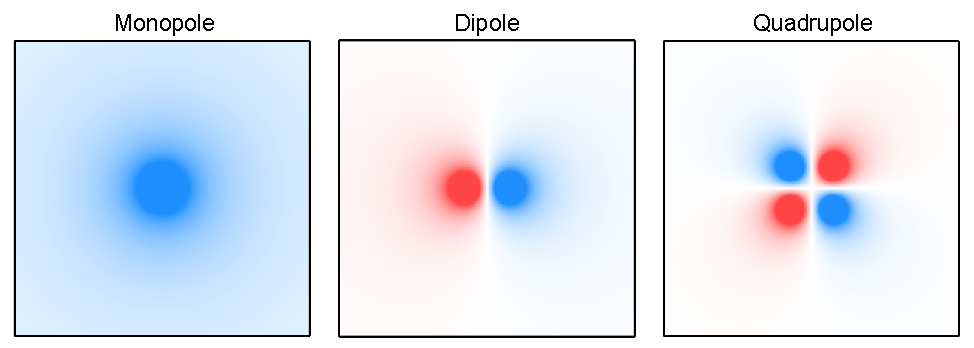
\includegraphics[width=88mm]{Figures/chapter1/multipole_expansion.pdf}
\vspace{-22pt}
\caption{\textbf{The first three terms of the multipole expansion.}}  \label{fig:multipole}
\end{wrapfigure}

The potential due to all current sources and sinks in a medium can be expressed as a multipole series expansion \cite{Nunez2006}. The first term in the series summarizes the \textit{monopole} contributions of all isolated sources and sinks. The current monopole corresponds to the net flow of current into or out of a volume and is equal in all directions. The second term is the contributions from current \textit{dipoles}, which are paired sources and sinks of equal magnitudes separated by an infinitesimal distance. Due to this specific arrangement, the currents cancel out and thus the dipole has no net monopole moment. The dipole instead expresses the directionality of current flow. The third term is the \textit{quadrupole} contribution. Analogous to the dipole, the quadrupole is the arrangement of four currents that together have no monopole nor dipole moment. These first three terms of the multipole expansion are illustrated in \autoref{fig:multipole}. 

The contribution of each pole to the electric potential decreases with distance, $R$, at a different rate \cite{Nunez2006}. Specifically,
\begin{equation*}
    \phi(R) = \frac{C_{monopole}}{R} + \frac{C_{dipole}}{R^2}  + \frac{C_{quadrupole}}{R^3}  + \dots
\end{equation*}
Because the sources and sinks of current are balanced throughout the brain, the monopole term is approximately zero for electric fields generated by macroscopic volumes of tissue \cite{Nunez2006}. Furthermore, for electrodes far away from the current densities, as is the case for EEG, the higher order terms contribute negligibly relative to the lower order terms. Consequently, EEG signals can be accurately modelled based on current dipoles alone \cite{Nunez2006,RevModPhys.65.413}. This gives us the following equation for the EEG signal \cite{RevModPhys.65.413}
\begin{equation} \label{eq:lead_solution}
    \phi_i(t) \approx \int_V \mathcal{L}_i(\bm{r}) \cdot \bm{Q}(\bm{r},t) dV(\bm{r})\mathrm{,}
\end{equation}
where $\bm{Q}$ is the current dipole moment at point $\bm{r}$ in the brain. 

\begin{figure}[b!]
    \centering
    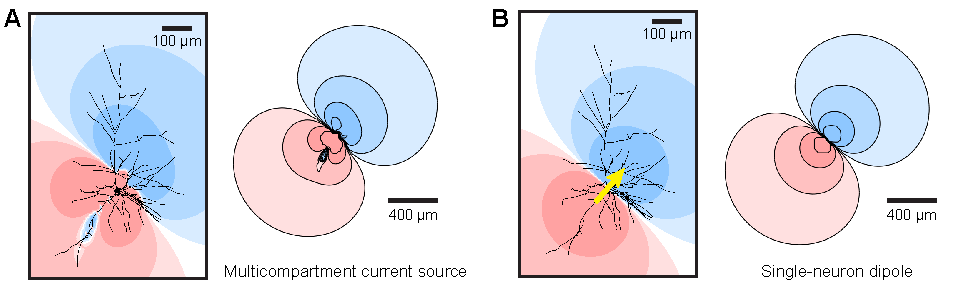
\includegraphics[width=\textwidth]{Figures/chapter1/single_neuron_dipole.pdf}
    
    \caption{\textbf{Single dipole approximation to the electric field generated by an individual neuron.} 
    (\textbf{A}) A multicompartment biophysical neuron model is simulated while receiving synaptic input. The left panel depicts the electric field surrounding the neuron at a moment in time. The right panel is the same simulation zoomed out twice as far (note the scale bars). Red and blue colours indicate positive and negative electric potential, respectively. (\textbf{B}) The electric field is modelled using a single dipole placed at the soma of the neuron (yellow arrow). The single-neuron dipole approximation does not capture the complexity of the electric field near the neuron, but provides a good approximation at further distances.} 
    \label{fig:single_dipole}
\end{figure}

Current dipoles can be modelled at multiple scales. Early work tended to model a neural mass with a single dipole ``mesosource'' that summarized the parallel alignment and synchronous activity of many current dipoles in a volume of neural tissue \cite{Nunez2006}. However, as knowledge grew about the role ionic conductances play in a neuron's electrical properties \cite{Baxter1991}, in tandem with expanding computational power \cite{Beeman2013}, more detailed biophysical models emerged of the current dipoles generated by individual neurons \cite{Murakami2002, Murakami2003 ,Murakami2006, Jones2007}. This led to the idea of a single-neuron dipole \cite{Næss2021,Pettersen2012}. While the morphology and distribution of currents strongly impact the extracellular electric field locally, far from the neuron, the totality of transmembrane currents can be approximated by a single dipole vector centered on the neuron (\autoref{fig:single_dipole}). The use of single-neuron dipoles in EEG modelling is a relatively recent development that provides a level of detail between mesoscopic dipoles, which reflect synchronized neural volumes, and microscopic current sources and sinks, which describe the detailed spatial distributions of transmembrane currents across a neuron. Single-neuron dipoles will play an important role in the modelling work of \autoref{sec:natcomms} and \autoref{sec:apEEG}.

\subsection{Head models of volume conduction} \label{sec:head_models}
After describing the distribution of current dipoles in the brain, the second part to modelling EEG signals comes from defining the lead field, $\mathcal{L}_i(\bm{r})$, at each point in the brain. This lead field must take into account the distribution of conductivity, $\sigma(\bm{r})$, so that the effects of volume conduction are properly modelled. The assumptions that go into calculating $\mathcal{L}_i(\bm{r})$ are together called a head model, i.e., a model that encapsulates all the effects of the head on volume conduction.

The simplest head model is to assume that we are measuring the electric potential inside an infinite, homogeneous volume conductor. Under this assumption, the electric potential at a point $\bm{r}^\prime$ generated by a dipole at a point, $\bm{r}$, is given by
\begin{equation}
    \phi(\bm{r}^\prime) = \frac{\bm{d} \cdot \bm{Q}(\bm{r})}{4\pi\sigma |\bm{d}|^3}\mathrm{,}
\end{equation}
where $\bm{d}=\bm{r}^\prime-\bm{r}$. Note that this equation is very similar to Coulomb's law for the electric field generated by static charges. This model is fairly reasonable for modelling the local field potential (LFP) \cite{Pettersen2012}, but it is a gross simplification for modelling EEG, as it neglects the large differences in conductivity between different tissues.

To capture this variation in conductivity, a popular model for EEG is the concentric spheres model. Under this model, the head is composed of concentric spherical layers of different radii and conductivity \cite{Geisler1961}. In the most accurate, four-sphere model \cite{Hosek1978}, the layers represent from inside out: the brain, cerebrospinal fluid, skull, and scalp. The major benefits of these models are that they (i) are more accurate than the infinite, homogeneous volume conductor model, and (ii) can be solved analytically, although the solutions are mathematically and notationally complex. A complete derivation and numerically validated solution to the four-sphere model is given by Næss et al. \cite{Næss2017}.

The most accurate models rely on numerical solutions to the Poisson equation (\ref{eq:poisson}) using techniques such as the finite element method. In this method, the problem domain is meshed into discrete ``elements'' upon which the solution is approximated with simple basis functions \cite{Liu2014}. In head modelling, this typically requires representing the various tissues of the head with a mesh of tetrahedral elements with each element assigned its own conductivity value \cite{Hallez2007} (\autoref{fig:FEM_mesh}{A}). Creating a head model for every subject in an experiment would require collecting MRI scans and defining a unique mesh for each subject, and is computationally intensive and impractical. Therefore, head models are typically based on the scan of a representative individual \cite{Holmes1998}. An improvement over this was introduced with the the New York Head model \cite{Huang2016}. In this model, Huang et al. \cite{Huang2016} constructed a mesh for the ICBM152 anatomical template that averages the MRI scans of 152 subjects, and included different conductivity values for six different tissue types: scalp, skull, cerebrospinal fluid, gray matter, white matter, and air cavities (\autoref{fig:FEM_mesh}B). Because this model represents an average head, the lead fields calculated by the model are proposed to be more generalizable than those calculated from a single representative individual \cite{Huang2016}. The New York head model comprises lead fields, $\mathcal{L}_i(\bm{r})$, for 231 electrode locations ($i\in\{1,2,...,231\}$) and for  ${\sim}75000$ cortical locations ($\bm{r}\in\{ \bm{r}_1, \bm{r}_2, ..., \bm{r}_{74382} \}$). These lead fields can be precomputed and stored, thus allowing high accuracy solutions to the forward EEG problem with low computational costs.

\begin{figure}[t!]
    \centering
    \includegraphics[width=\textwidth]{Figures/chapter1/head_models.pdf}
    
    \caption{\textbf{Head models using the finite element method.} 
    (\textbf{A}) Example triangular mesh of a coronal section of the head used for finite element modelling. Figure adapted from Hallez et al. \cite{Hallez2007} under a Creative Commons license. © 2007 Hallez et al; licensee BioMed Central Ltd. (CC BY 2.0).
    (\textbf{B}) Segmentation of the New York head model into six tissue types: scalp (\textbf{a}), skull (\textbf{b}), cerebro-spinal fluid (\textbf{c}), gray matter (\textbf{d}), white matter (\textbf{e}), and air cavities (\textbf{f}). The location of 231 electrodes are shown on the scalp in panel (a). Figure adapted from Huang et al. \cite{Huang2016} under a Creative Commons license. © 2016 Huang et al (CC BY 4.0).
    } 
    \label{fig:FEM_mesh}
\end{figure}

\section{The standard model of EEG} \label{sec:standard_model}

\begin{wrapfigure}[16]{r}{80mm}
\vspace{-15pt}
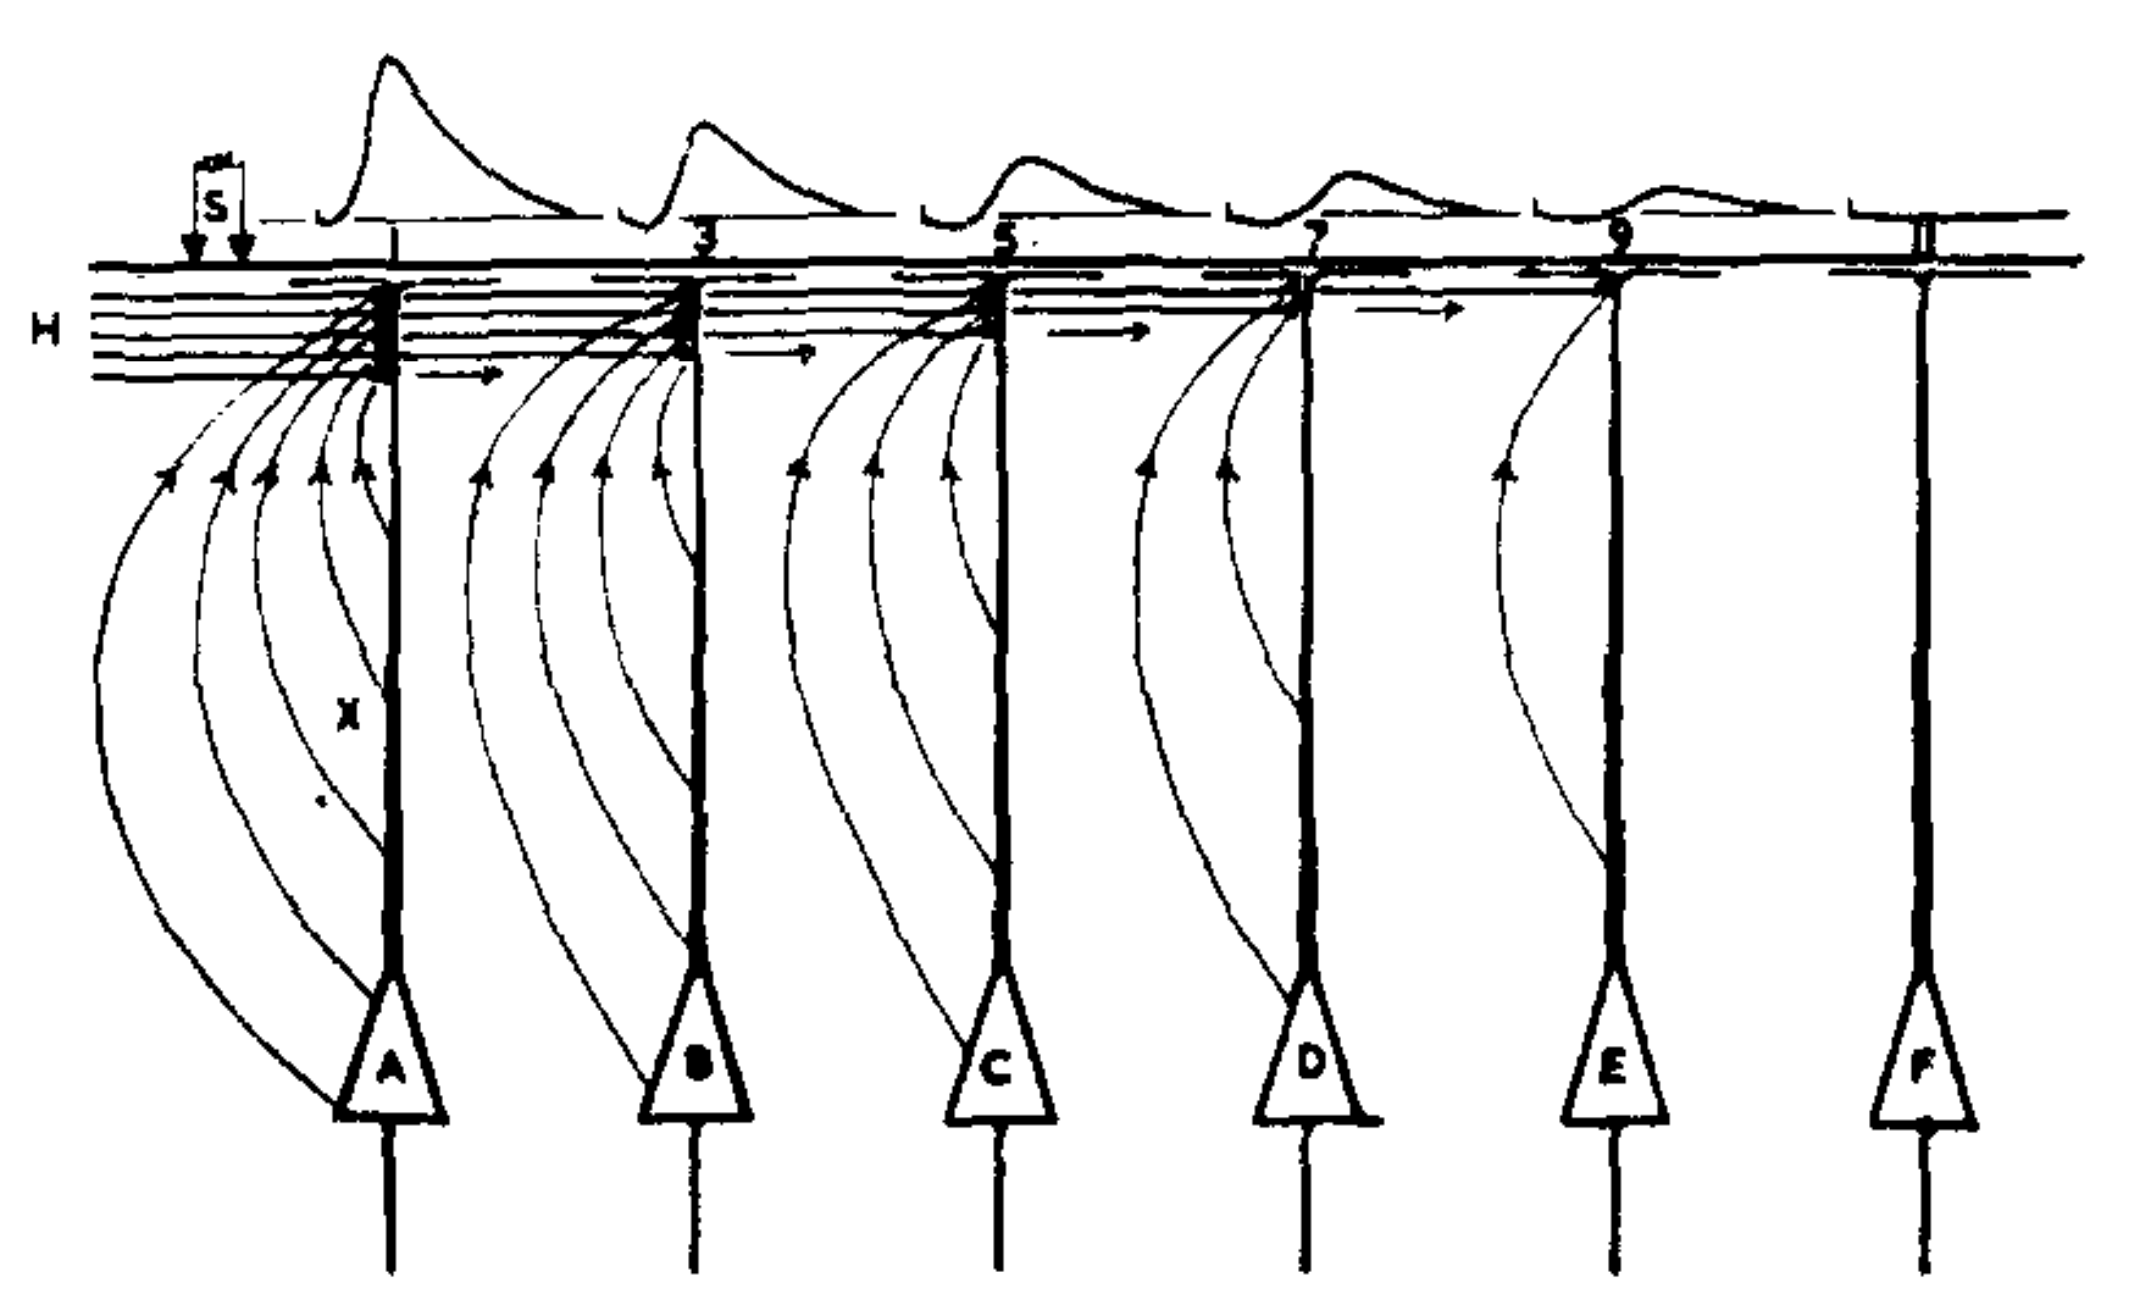
\includegraphics[width=80mm]{Figures/chapter1/Eccles_1951.png}
\vspace{-20pt}
\caption{ \captiontitle{Early model of EEG generation by Eccles (1951).} Surface potentials (transients drawn the top of the figure) are induced by cortical simulation of layer 1 axons. The spreading excitation of the apical dendrites of pyramidal neurons generates open field configurations that are aligned in parallel. The fields are represented by the curved lines around each dendritic trunk. Reprinted from Electroencephalography and Clinical Neurophysiology, Vol 3/4, J.C. Eccles, Interpretation of action potentials evoked in the cerebral cortex, Pages No. 449-464, Copyright (1951), with permission from Elsevier.
} \label{fig:eccles}
\end{wrapfigure}

The foregoing overview explains how currents in neural tissue produce scalp potentials, but not why the brain generates EEG signals. In addition to the biophysics of EEG, there are two key neural features important for EEG generation: geometry and dynamics. In order to generate electric fields large enough to be detected at the scalp, ion channels must be generating current dipoles that are coherent \cite{Buzsaki2012, Nunez2006}, and because dipoles are vectors, this means that both the temporal dynamics and the spatial configuration of these dipoles must be correlated. The following description reflects the standard textbook explanation of EEG. The reason for saying this is because some of the theories concerning the EEG spectral trend to be discussed do not follow this textbook explanation.

\subsection{Pyramidal cells and synaptic currents}

Based on early experimental observations of how superficial potentials propagate following cortical simulation, mid-century electrophysiologists \cite{Eccles1951} reasoned that the EEG signal is likely generated by excitatory synaptic inputs onto the apical dendrites of pyramidal neurons (\autoref{fig:eccles}). This was controversial at the time, as others still believed that the signal primarily reflected action potentials \cite{Burns1950}. It was later confirmed through cross-correlation analysis that postsynaptic potentials and the EEG signal are statistically related \cite{KLEE1965}. Broadly, the synaptic current model became the canonical viewpoint, and notably provides both of the necessary mechanisms for EEG generation: (i) synaptic currents last longer than action potential and therefore overlap more in time, increasing the chance of a superposition of current dipoles; and (ii) because of the parallel orientation of pyramidal neurons, synchronized synaptic input into their apical dendrites should generate similarly oriented dipoles.

Early work debated how much EEG signals reflected excitatory versus inhibitory postsynaptic potentials \cite{Pollen1964,Creutzfeldt1966, Creutzfeldt1966a}. It is typically thought that inhibitory synapses are primarily concentrated on the soma \cite{Telenczuk2020, Mazzoni2015,Næss2021}, where transmembrane currents generate small current dioples \cite{Ahlfors2015}. Furthermore, the reversal potential of GABA receptors is closer to the resting membrane potential of the cell, and it has thus been argued that they do not generate as large currents \cite{Buzsaki2012}. However, more recent experimental observations show that neither of these arguments are entirely true. Firstly, inhibitory cells do in fact target the apical dendrites of cortical pyramidal neurons \cite{Palmer2012}. In fact, recent whole-cell synapse mapping shows that inhibitory synapses are more or less uniformly distributed across the entire dendritic arbour \cite{Iacaruso2017}, although still highly concentrated on the soma. Secondly, in vivo neurons are constantly bombarded by excitatory and inhibitory synaptic input, meaning that their membrane potential is not at rest as it is in vitro \cite{Destexhe2003}. The driving force of GABA and AMPA receptors during this high conductance state is much more balanced than seen in experiments in vitro. It is generally considered now that both excitatory and inhibitory synaptic currents contribute to EEG signals \cite{Buzsaki2012}. Nonetheless, many studies of network dynamics still only consider the excitatory synaptic currents when modelling the EEG signal \cite{Jensen2005,McCarthy2008}, and the relative contribution of these two types of currents to EEG signals is far from established. In sum, although every transmembrane current contributes to extracellular potentials, typically only currents mediated by AMPA (and sometimes GABA) receptors are considered as the generators of EEG rhythms.

\subsection{Synchrony through rhythmicity}  \label{sec:delta}
If neurons all fire randomly, their electric fields would not sum together in any appreciable way and no EEG signal would transpire. Enter brain rhythms. Neurons are fundamentally oscillators \cite{HODGKIN1952} and oscillators like to synchronize \cite{Strogatz2015}. In fact, it is often difficult to \textit{stop} coupled oscillators from synchronizing \cite{Erb1992}. It is perhaps not surprising therefore that the brain exhibits synchronized oscillations of neurons. These oscillations in turn produce synchronized postsynaptic currents in large pyramidal cells, giving rise to detectable oscillations on the EEG. This is the so-called ``standard model'' of EEG \cite{Cohen2017}. However, there is nothing standard about the wide range of frequencies, neural assemblies, and synchronizing mechanisms that characterize the repertoire of neural oscillations observed in the brain.

The first brain rhythm that was observed was the alpha rhythms (8 to \qty{12}{\hertz}) \cite{Berger1929}, which appears during idleness \cite{Adrian1934}; however, the rhythm may in fact reflect an active inhibition of non-task relevant cortical areas \cite{Cooper2003}. The next rhythms that became apparent are those that are observed during sleep \cite{Loomis1937,Weber2016} and general anesthesia \cite{GIBBS1937,Akeju2017}. Both states share the appearance of delta oscillations ($<4$ \unit{\hertz}), although this rhythm may be caused by distinct underlying mechanisms in sleep and anesthesia \cite{Akeju2017}. Then, there are the rhythms that have been linked to information processing and cognition in awake, behaving humans, including the beta (15 to \qty{30}{\hertz}) \cite{Spitzer2017} and gamma rhythms (30 to \qty{50}{\hertz}) \cite{JASPER1938,Fries2009}. While alpha, beta, delta, and gamma rhythms are perhaps the most notable, there are in fact many more rhythms that have been observed and which span almost the entire frequency range from \qty{0.1}{\hertz} up to \qty{600}{\hertz} \cite{Penttonen2003}. To highlight the diversity in neural rhythms, I will briefly review the neural mechanisms thought to underlie just two of these rhythms: the delta rhythm during sleep and the gamma rhythm observed during wakefulness.

\subsubsection{Example 1: delta rhythms}
Delta rhythms are an intrinsic oscillation of thalamocortical neurons. When these neurons are hyperpolarized to levels below $-65$ to $-70$ \unit{\milli\volt} in vivo, the cells switch from a tonic firing to a bursting regime with a frequency between 0.5 and \qty{4}{\hertz} \cite{Dossi1992}. This bursting activity is characterized by subthreshold oscillations reflecting the interplay of a non-inactivating, hyperpolarization-activated inward current, the h-current, and a low-voltage activated calcium current, the t-current \cite{McCormick1990,Soltesz1991}. These thalamocortical neurons make reciprocal connections with the inhibitory reticular thalamic neurons and this population-level negative feedback is thought to synchronize the oscillations of each thalamocortical neuron \cite{Steriade1991, Steriade1993}. In the waking state, input from the active cholinergic system depolarizes the membrane potential of thalamocortical neurons out of the range of bursting and prevents delta oscillations \cite{Steriade2003}. However, during non-REM sleep, the acetylcholine system is suppressed \cite{Watson2010}, and the resulting lack cholinergic input from the brainstem is thought to let thalamocortical neurons fall into their bursting regime \cite{Steriade2003}. Ultimately, this thalamocortical rhythm produces synchronized excitatory synaptic currents in the cortex, giving rise to the delta oscillations on the EEG during non-REM sleep \cite{Amzica1998}.

\subsubsection{Example 2: gamma rhythms}
 Gamma rhythms have been most completely described in the hippocampus and visual cortex, where it can be evoked by spatial exploration \cite{Bragin1995} and visual attention \cite{Gray1989}, respectively. Unlike the delta rhythm explained above, the gamma rhythm is not an intrinsic property of the constituent neurons. Also unlike the delta rhythm, the gamma rhythm is generated entirely intracortically \cite{Gray1989} and can be examined in vitro using acute cortical slices \cite{Whittington1995}. Such slice work revealed that, mechanistically, gamma oscillations only require a population of reciprocally connected interneurons receiving sufficient excitatory drive \cite{Whittington1995, Buzski2012b}. Indeed, blocking GABA\textsubscript{A} receptors universally prevents gamma oscillations in slices \cite{Bartos2007}. Computational modelling validated that networks comprised entirely of interneurons can synchronize into a gamma rhythm \cite{Wang1996}. It was thus argued that interneuron gamma oscillations create coherent, subthreshold oscillations in pyramidal neurons that in turn synchronize their excitatory outputs, leading to a gamma oscillations on the EEG \cite{Wang1996}. There is also a model of gamma oscillations that requires excitatory connection, the so-called E-I model, as opposed to the foregoing I-I model \cite{Buzski2012b}. In this model, oscillations are generated by alternating excitatory firing followed by delayed reciprocal inhibition \cite{Borgers2003}. This model is also supported by experimental evidence. For example, depending on the pharmacological intervention used to excite interneurons in a slice, blocking AMPA receptors can also prevent gamma oscillations \cite{Bartos2007}. Regardless of the model, it is agreed that gamma oscillations emerge from the local interactions among cortical neurons and that the rhythm's frequency is determined by the timescales of inhibitory currents \cite{Bartos2007, Buzski2012b}.

\subsection{Summary}
In the standard model, EEG reflects populations of excitatory neurons that are entrained to an oscillation. This oscillation synchronizes postsynaptic excitatory currents in pyramidal cells, thus generating widely correlated current dipoles. The mechanisms that produce synchronous oscillations in neurons are diverse and the spatial scale over which this synchrony is exhibited can vary from patches of the cortex to the entire thalamocortical system. The standard model focuses on EEG rhythms and does not provide an obvious explanation for the EEG spectral trend.

\section{Existing theories on the spectral trend} \label{sec:theories}

\subsection{Theory 1. Local versus global synchrony: the classical view} \label{sec:all_oscillations}

The first theory on the EEG spectral trend follows in the tradition of the standard model of EEG and argues that, as EEG reflects brain rhythms, the spectral trend must reflect a particular organization of brain rhythms; the brain does not produce broadband EEG signals, but rather a broad and continuous range of oscillatory signals. According to this theory, the slope of the EEG spectrum is a conflated measure of many different brain rhythms and is not a unified feature of EEG. Instead, EEG spectra appear to exhibit $1/f$ scaling for the following reasons.

\begin{wrapfigure}[9]{T}{65mm}
\vspace{-10pt}
\centering
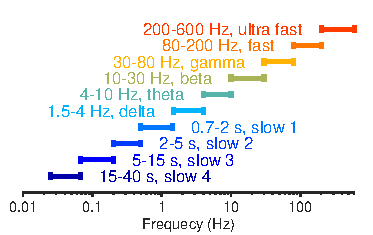
\includegraphics[width=60mm]{Figures/chapter1/rhythm_frequencies.pdf}
% \vspace{-5pt}
\caption{\textbf{The progression of neural oscillations described by Pentoonen and Buzsáki}\cite{Penttonen2003}.}  \label{fig:osc_prog}
\end{wrapfigure}

First, the brain exhibits a wide and diverse repertoire of oscillations that spans a large frequency range. On the lower end of the frequency scale, slow $<1$ \unit{\hertz} EEG oscillations are apparent during sleep \cite{Achermann1997}. On the other end of the scale, ultra-fast oscillations from 200 to 600 Hz were found in the local field potential of the somatosensory cortex of sleeping rats \cite{Kandel1997}, and also appear in human EEG, particularly in patients with epilepsy \cite{Frauscher2017}. In fact, a systematic review found brain oscillations that cover the entire range of frequencies between these two extremes \cite{Penttonen2003}. Moreover, on a logarithmic frequency scale, it was found that oscillations provide continuous and linearly spaced coverage with little overlap (\autoref{fig:osc_prog}). For example, lower frequency oscillations, such as delta rhythms which range from $\sim$1.5-4 Hz, cover a range of a couple hertz, whereas high frequency oscillations, ranging from 200 to 600 Hz, cover a range of several hundred \cite{Penttonen2003}. 

Second, it is argued that slower oscillations recruit larger assemblies of neurons than faster oscillations \cite{Buzsaki2006, Buzsaki2012c, Buzsaki2010}. This argument is based on a theory of temporal coding, the concept that neurons, or assemblies of neurons, encode information through the precise timing of action potentials. Due to conduction delays, it is argued that communication among spatially broad ensembles of neurons must have more tolerance in signal timing (``obtaining a global consensus takes more time'' \cite{Buzsaki2006}), and are therefore organized into slower oscillations. On the other hand, local processing has short conduction speeds and can therefore be more temporally precise and are organized into faster oscillations. During cognitive tasks requiring multiple brain regions, it was shown that long range coherence among EEG channels indeed appeared at lower frequencies \cite{Sarnthein1998,VonStein1999}, whereas LFP and unit recordings have revealed fast, local gamma synchrony among primary visual neurons upon visual stimulation in monkeys and cats, which is believed to be related to local processing in the visual cortex \cite{Gray1989,Eckhorn1994}.

Third, volume conduction acts as a spatial low-pass filter \cite{Nunez2006} and therefore EEG signals are biased by neural activity that is coherent over larger regions of the cortex. In other words, the temporal frequencies characteristic of large spatial scales will be amplified in EEG. In conjunction with the arguments in the foregoing paragraph, one should expect an EEG signal that is dominated by widely synchronized, slow oscillations, while faster oscillations, even if they are widespread, are only locally synchronized and therefore contribute significantly less. Extrapolating this argument to the entire continuum of oscillations described by Pentoonen and Buzsáki \cite{Penttonen2003} and one would expect to see an EEG spectrum which decays linearly in amplitude on a logarithmic frequency scale, essentially giving rise to the appearance of a 1/f trend.

Adding to these phenomena is the argument that EEG spectra tend to be averaged over many trials or calculated over long periods of time (e.g., \qty{86}{\min} in \autoref{fig:phenomenology}B). However, the state of the brain is constantly evolving and the various rhythms come and go. Therefore, computing EEG spectra over long periods of time, multiple individuals, or different tasks produces spectra that have no clearly obvious peaks as these distinct rhythms have blured together into a continuous spectrum \cite{Buzsaki2006}.

\subsubsection{Caveats}
A drawback to this theory is that, while many oscillations have clearly been found in the brain, there is scant evidence that they are all working together at the same time in healthy, waking and behaving humans. For example, many of these slow oscillations have only been described in sleeping or anesthetized states \cite{Hromadka2013}. Even in a recording lasting a couple of minutes in awake humans, it is unclear why such rhythms mights manifest. Moreover, there is direct evidence, at least in LFP data, that broadband signals do in fact exist; Ray and colleagues showed that increases in the high gamma frequency ranges (80-150 Hz) following visual stimulation is a direct reflection of broadband spiking activity and not rhythmic activity \cite{Ray2008,Ray2011}. 

Furthermore, the central tenet that fast oscillations are locally synchronized and slow oscillations are globally synchronized, while supported by some evidence, still lacks the type of robust experimental observations required to argue this point as a fundamental operating regime of the cortex \cite{Buzsaki2006}. For example, during sleep, it was shown that slow wave oscillations are synchronized over large regions (at least 7 mm), whereas faster oscillations are more locally coherent, with their spatial correlations decaying over just a couple of millimeters \cite{Destexhe1999}. However, faster oscillations were also sometimes observed to be synchronized over 7 mm as well, indicating that there are neural mechanisms for spatially extended synchrony of fast oscillations \cite{Destexhe1999}. Conversely, under propofol anesthesia, the brain exibits slow delta oscillations, but these oscillations are only locally synchronized across less than \qty{4}{\milli\meter} \cite{Lewis2012}. Overall, while there is circumstantial evidence that rhythm frequency is inversely proportional to the size of the neuronal pool, there has been no quantification of this phenomenon per se and it is unclear whether this concept can actually explain the EEG spectra trend quantitatively.

\subsubsection{Summary}
In summary, while this holistic theory of brain oscillations likely explains in part the 1/f appearance of EEG spectra, especially when spectra are averaged over long periods of time, its foundational doctrines still lack some necessary experimental evidence. It also does not provide a clear answer to how the EEG spectral trend should be dealt with. Buszaki, a proponent of this theory, suggests that EEG spectra can be whitened to remove the apparent 1/f trend \cite{Buzsaki2006}. However, if all the power is indeed due to oscillations, it is unclear why this detrending procedure should be applied at all. Broadly, this theory questions the utility of measures like the spectral exponent. Therefore, if one wishes to claim that the spectral trend provides novel insights complementary to the traditional analysis of EEG rhythms, this is the theory to beat.

\subsection{Theory 2. Self-organized criticality: evidence and controversy} \label{sec:SOC}

Historically, the primary opponent to the above classical view is the theory of self-organized criticality, an alternate model of brain function that invokes a theory developed to explain the ubiquity of power law scaling in nature. Of all the theories reviewed here, that of self-organized criticality is perhaps the most elaborated, controversial, and passionately stated. This passion might partially be due to its proponents viewing power laws with a ``vague and mistakenly mystical sense of universality'', to quote Stumpf and Porter’s perspective piece in \textit{Science}\cite{Stumpf2012}, and is certainly due in part to the theory’s genuinely elegant implications for brain function, such as optimizing dynamic range \cite{Kinouchi2006} and information transmission \cite{Shriki2016}. Like the theory in \autoref{sec:all_oscillations}, the idea of self-organized criticality is principally a theory about brain function, but has also been used to explain the apparent broadband signals in macroscopic neural recordings. 

Many systems appear to exhibit power-law scaling, from earthquakes to forest fires to the stock market. Forty years ago, a now seminal paper by Bak et al. \cite{Bak1987} proposed an explanation for this seemingly universal phenomenon. It was known in statistical physics that systems at second-order phase transitions exhibit power-law scaling in both time and space \cite{pathria2016statistical}. But the parameter regime of this phase transition is infinitesimally small; how could systems everywhere be perched at this delicate point? The theory of self-organized criticality illustrates that certain systems spontaneously tend towards this critical point, by virtue of the complex interactions of the system's constituents, i.e., the critical point is a stable state of the system. Bak et al. \cite{Bak1987} exemplified this with a simple cellular automaton model. Cells are laid out in a lattice and each is associated with a number value. If a cell’s value exceeds a threshold, then a value of one is transferred from the cell to each of its neighbors. When initializing values randomly, the system will eventually settle into an equilibrium state, but one which is extremely sensitive to perturbation. Tripping just one of the cells will send off a so-called ``avalanche'', whose size, $S$, was shown to be distributed as a $1/S^\beta$ power law. In his book, \textit{How Nature Works}\cite{Bak1996}, Per Bak argues that ``the complex phenomena observed everywhere indicate that nature operates at the self-organized critical state.''

The parallels between the original cellular automaton model and neural networks are quite apparent. When a neuron’s excitatory input reaches a certain threshold, the cell fires an action potential, which causes an excitatory potential in each of the cell’s postsynaptic partners (assuming all neurons are excitatory). Consequently, there was much early interest among physicist in applying the theory of self-organized criticality to the brain \cite{Corral1995, Herz1995}. While these original studies on simulated neural networks needed to tune parameter values to achieve a critical process, it was later shown that a network of excitatory integrate-and-fire neurons will self-organize into a critical state with the addition of synaptic depression \cite{Levina2007}. It was also shown that networks of excitatory and inhibitory integrate-and-fire neurons exhibit avalanche criticality when excitation and inhibition is particularly balanced \cite{Poil2012, Lombardi2017}. In brief, there were many early studies suggesting that self-organized criticality is theoretically possible in neural networks.

Accordingly, it was also suggested that self-organized criticality underlies the power-law scaling observed in macroscopic neural recordings \cite{Lombardi2017}. Indeed, the average height, $S$, of an avalanche is related to its duration, $T$, as $S(T)\propto T^{1/\sigma\nu z}$, with the consequence that the system's spectrum should also follow a power-law \cite{Kuntz2000} (the exact meaning of the parameters $\sigma$, $\nu$, and $z$ are not relevant for our discussion but are defined by Kuntz and Sethna \cite{Kuntz2000}). It has been shown that simulated networks of excitatory and inhibition neurons at criticality generate neuronal avalanches with a spectral exponent $\beta\in[1,2]$ depending on the percentage of inhibitory synapses in the model \cite{Lombardi2017}. Given its theoretical interest, what evidence is there that the brain is actually operating in a self-organized critical state?

At the turn of the millennium, Beggs and Plenz \cite{Beggs2003} tested whether slices of brain tissue exhibit cascades of action potentials that obey the dynamics of a self-organized state. Organotypic and acute slices were studied on an electrode array and negative deflections at each electrode, indicative of locally synchronized spiking, were analyzed. These experiments were the first to show that cortical circuits can exhibit so-called neural avalanches – cascades of activity with sizes and durations that obey power laws. Indeed, it was found that the activity was consistent with a branching process (see \hyperref[box:first]{Box 1}). Later, neuronal avalanches consistent with a branching process were also identified in LFP recordings in monkeys in vivo, indicating that this phenomenon may indeed play a role in physiological brain dynamics \cite{Petermann2009}. Power-law relations have since been identified across many species using many different recording modalities, including voltage \cite{Scott2014} and calcium imaging \cite{Bellay2015,Ponce-Alvarez2018}.

\begin{mybox}[floatplacement=t,label={box:first}]{Definition of branching process}
   A \textit{branching process} describes the evolution of a population of individuals, whereby at the end of a generation, each individual dies and leaves behind a certain number of offspring. In a neural network, these individuals are taken to be action potentials and the offspring are the subsequent action potentials elicited in postsynaptic partners. The dynamics of a branching process are determined by the branching number, $m$, that reflects the average number of offspring per individual. Branching processes are often modelled with immigration, that is at each generation, a number of individuals, $h$, are added to the population in addition to the offspring. Mathematically, the population size at a given time point, $A_t$, is given by the following recursive equation \cite{Wilting2018}
    \begin{equation}
        A_{t+1} = \sum_{i=1}^{A_{t}} y_{i,t} + h_t\mathrm{,}
    \end{equation}
    where $y_{i,t}$ is the number of offspring for individual $i$ of generation $t$.  $y_{i,t}$ are independent and identically distributed according to some law $y_{i,t}\sim\mathcal{Y}$, with mean $\mathbb{E}(\mathcal{Y})=m$. If the branching number is $m>1$, then the population size, e.g., number of action potentials, will increase exponentially and without bound. If the branching number is $m<1$, the population size will reach a stable steady-state, $A_{\infty}=h/(1-m)$. Thus, a parameter value of $m=1$ is a critical point of the system. Notably, as $m\to1$, the number of individuals will exhibit avalanches with a size distribution that approaches a power law with a slope of $-3/2$, exactly that observed by Beggs and Plenz \cite{Beggs2003}.
\end{mybox}


\subsubsection{Caveats}

Despite the explosion of papers on self-organized criticality in the brain over the past two decades, the topic remains highly controversial. One caveat to these studies is the lack of strong statistical evidence for power laws. For example, to conclude there is a power law in a probability distribution, this scaling should continue over at least two decades of the variable and should be estimated with maximum likelihood estimation \cite{Stumpf2012}. Secondly, there should be an actual statistical test of whether the relationship is best explained by a power law. Few of the foregoing studies performed robust statistical analyses on their avalanche distributions \cite{Clauset2009}. The most convincing analyses are from calcium imaging studies \cite{Bellay2015, Ponce-Alvarez2018}. However, due to the slow kinetics of calcium indicators, the avalanche power spectrum can only be computed for very low frequencies, less than 1 Hz in the case of Ponce-Alvarez et al.\cite{Ponce-Alvarez2018}, and therefore unfortunately do not provide much information on the EEG spectral trend in the frequency range typically of interest.

The requirement for a power law over two decades of data is a particularly strong caveat in tying self-organized criticality to EEG, as a look through the literature on EEG spectra reveals a hodge-podge of power law measurements, which typically rely on simple linear regression and are often over short segments of spectra: $\beta=2$ from 30 to 50 Hz \cite{Lendner2020}; $\beta=1.4$ from 0.15 to 9.5 Hz \cite{Dehghani2010}; $\beta=1.3$ from 0.5 to 30 Hz \cite{Pritchard1992};  $\beta=-1$ from 1 to 40 Hz \cite{Colombo2019}; $\beta\in[1,3]$ from 3 to 30 Hz \cite{Pereda1998}. This is by no means an exhaustive list. One likely reason for these varied and often short frequency ranges is the difficulty in estimating power laws from the whole spectrum; EEG spectra clearly exhibit peaks due to narrowband neural activity, and it is unclear how these peaks should be accounted for when measuring purported power laws. These peaks are either entirely ignored and included in the power-law fit (\autoref{fig:phenomenology}A), or the spectra are averaged over such long periods of time that the peaks are blurred to the point of nonrecognition. Even a ``short'' time window of 20 s (as used for validation by He et al.\cite{He2010}; $\beta\in[2,3]$ from 1 to 100 Hz) contains at least 1000 periods of an oscillation above \qty{50}{\hertz}, over which time the oscillation may disappear and reappear or fluctuate widely in frequency. Consequently, there is very high potential for the blurring of spectral peaks, and scaling at these frequencies may therefore be an epiphenomenon of purely rhythmic activity. In fact, such a blurring of spectral peaks at various frequencies is essentially the argument outlined above in \autoref{sec:all_oscillations} and is clearly not consistent with self-organized criticality. Even methods that claim to account for rhythmic EEG components measure different spectral exponents from the same spectrum (\autoref{fig:gerster}).  In sum, the evidence of power-law scaling in EEG spectra is inconsistent and the actual value of the spectral exponent is very poorly defined. 

A second caveat to assessing criticality in the brain is that the nature of in vivo electrophysiological measurements severely undersamples the neuronal population, which prevents accurate inference of power laws and branching numbers \cite{Priesemann2009}. Even imaging studies often only genetically express calcium or voltage indicators in a subset of neurons, such as layer 2/3 pyramidal cells \cite{Scott2014,Bellay2015}. One study was performed in transgenic zebrafish \cite{Ponce-Alvarez2018}; however, despite expressing GCaMP under a pan-neuronal promoter, transgenic expression is often incomplete and highly variable between cells. Therefore, even measurements of ``whole-brain dynamics'' still suffer from subsampling. Recent theoretical advances have provided statistical tools for accurately inferring branching numbers from undersampled systems \cite{Wilting2018}. Applying these statistical tools to in vivo electrophysiological recordings have suggested that the cortex does not operate at criticality, but rather in a subcritical regime, with a branching number calculated to be between 0.95 and 0.998 \footnote[2]{This might not seem far off from $m=1$. However, as pointed out by Wilting and Preisemann\cite{Wilting2019}, the susceptibility of the system to external perturbation is $\partial A/\partial h = \frac{1}{1-m}$, indicating that the overall dynamics are extremely sensitive to small differences in the branching number around the singularity $m=1$.} in monkeys, cats, mice \cite{Wilting2018,Wilting2019} and zebrafish \cite{Suryadi2022}. Interestingly, it has been noted that the purported computational properties that are maximized at criticality also come with trade-offs, such as poor reliability \cite{Gollo2017} and critical slowing down \cite{Scheffer2012, Wilting2019a}. Therefore, it has been suggested that a slightly subcritical dynamical regime may in fact balance the various computational tasks of the cortex better than it would at criticality \cite{Wilting2019a}.

A final caveat to this theory is that the EEG signal is not a measure of the average firing rate of a network (\autoref{sec:EM_theory}). Therefore, the spectrum of neural avalanches, or even subcritical dynamics, does not immediately translate into the spectrum of the EEG. None of the studies discussed above attempted to simulate the electric fields potentially generated by their modelled neural networks.  Therefore, as in the previous theory, it is unclear whether this theory quantitatively explains the scaling observed in EEG spectra.

\subsubsection{Summary}

Self-organized criticality is a theory about the dynamical regime in which cortical networks operate, which has been claimed to confer special computational advantages. However, the evidence that the brain operates at a self-organized critical point is controversial. The most statistically sound evidence comes from estimating the branching number (\hyperref[box:first]{Box 1}) from in vivo spike recordings, which has consistently indicated that the brain operates below criticality. What does this all mean for the EEG spectral trend? It is clear from the above evidence that the cortex can operate in an aperiodic regime characterized by cascades of neural activity, regardless if these cascades obey a strict power law. This observation casts some doubt on the standard model of EEG, which assumes that all synchronous activity occurs through neural oscillations. The basic question of whether subcritical network dynamics are capable of generating detectable EEG signals remains surprisingly unaddressed. 

\subsection{Theory 3. Synaptic timescales: unchallenged and underexplored} \label{sec:timescales}

In their paper ``Does the 1/f Frequency Scaling of Brain Signals Reflect Self-Organized Critical States?'', Bedard et al.\cite{Bedard2006} presented an early challenge to the hypothesis that EEG spectra indicate self-organized criticality and proposed an alternate explanation. The authors performed inter-spike interval and avalanche analysis on isolated spikes measured with bipolar extracellular electrodes in waking and sleeping cats, and found that the statistics of spiking were almost perfectly captured by a Poisson process \cite{Bedard2006}. To model the simultaneously measured LFP signal, the authors convolved the recorded spike trains with an exponentially-decaying synaptic response, generating a spectrum with an exponent of $-2$. The authors argued that the scaling observed in LFP spectra results from the filtering of an essentially white-noise process by the kinetics of postsynaptic potentials. Because convolution becomes multiplication in Fourier space, the power spectrum of this system is
\begin{equation}
P(f) =|\hat{C}(f)|^2 \frac{\tau^2} { 1+ (2\pi\tau f)^2}\mathrm{,}
\end{equation}
where $\tau$ is the decay time constant of the synaptic current (set to be $\tau=10$ \unit{\milli\second} by the authors), and $|\hat{C}(f)|^2$ is the power spectrum of the ``drive'' signal, which in the case of a homogeneous Poisson process is simply equal to the mean rate. Thus, if macroscopic recordings (LFP and EEG) reflect postsynaptic currents, the timescale of these responses should shape the signals' spectra. Notably, the authors found that their LFP spectra scaled with an exponent of $-3$ above 20 Hz. This ``missing'' 1/f factor was attributed to filtering of the signal through neural tissue (see \autoref{sec:filter_theory} below).

Later Miller et al. \cite{Miller2009} published a similar model for electrocorticographic (ECoG) recordings \footnote[2]{ECoG is similar to EEG but the electrodes are placed on the surface of the dura. It is an invasive recording that measures EEG signals intracranially.}. Spectra averaged over several minutes of data indicated an exponent of $-4$ at frequencies above 80 Hz. They argue, similarly to Bedard et al., that a $1 / (1+ (2\pi\tau f)^2)$ factor is contributed by the decay kinetics of synaptic currents (these authors fit their spectra with $\tau=4$ \unit{\milli\second}), while the additional $-2$ factor was explained in a mathematically similar way, with a leak current that restores the membrane potential with a slow time constant of \qty{100}{\milli\second}.

In short, both papers argue that synaptic currents significantly shape the spectra of macroscopic recordings, but disagree over how much additional filtering is exhibited and what the mechanism underlying this additional filtering may be. There is significant experimental evidence that postsynaptic potentials are the primary sources of LFP and EEG, making the core argument of these papers highly plausible. However, as described in \autoref{sec:standard_model}, experimental evidence largely points to both excitatory and inhibitory currents as sources of EEG signals. It is therefore interesting that both studies only fit their spectra with a single synaptic timescale and moreover that Miller et al. \cite{Miller2009} found a timescale that more closely matched the kinetics of AMPA receptors, whereas the timescale from Bedard et al. \cite{Bedard2006} more closely matched the kinetics of GABA receptors (\autoref{sec:I_syn}).

Gao et al. \cite{Gao2017} were seemingly the first to explicitly consider the scaling imparted by both inhibitory and excitatory currents. The authors modelled macroscopic recordings with the same model as Bedard et al. \cite{Bedard2006}, except that Gao et al. considered two processes, one filtered by inhibitory synapses and another filtered by excitatory synapses. This simple extension led to an important insight. Because these two processes are filtered by different time constants, they contribute to the spectrum in different frequency ranges. In particular, because GABA receptor kinetics are slower than AMPA receptor kinetics, the inhibitory process contributes power preferentially at low frequencies (\autoref{fig:gao}). Consequently, if the synaptic excitation to inhibition (E:I) ratio decreases, e.g., if inhibition increases in amplitude, there will be an increase in the spectrum specifically at lower frequencies. The authors concluded that the synaptic E:I ratio determines the spectral exponent between 30 and 50 Hz, a range determined jointly by the time constants of excitatory and inhibitory synaptic decay (\autoref{fig:gao}).

\begin{wrapfigure}[16]{r}{65mm}
\vspace{-20pt}
\centering
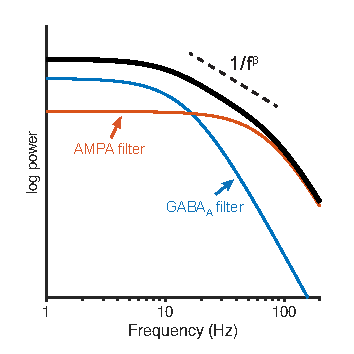
\includegraphics[width=60mm]{Figures/chapter1/EI.pdf}
\vspace{-14pt}
\caption{\textbf{Synaptic timescale hypothesis with excitation and inhibition.} Gao et al. \cite{Gao2017} hypothesized that if macroscopic neural recordings reflect synaptic currents, the signal will be filtered by an AMPA receptor filter (red) and GABA receptor filter (blue). The spectrum of the recording (black) will exhibit a spectral exponent determined by the relative contribution of excitatory and inhibitory currents.}  \label{fig:gao}
\end{wrapfigure}

As described above, there is strong experimental evidence that the macroscopic electric fields generated by the brain reflect primarily postsynaptic currents, making this theory highly plausible. However, this theory does have important caveats. Firstly, all of the studies described above modelled the field as a filtered Poisson process, i.e., there was no synchrony assumed in any of the models. Miller et al.\cite{Miller2009} argued explicitly that the spectral trend reflects ``asynchronous'' brain signals. This is clearly at odds with the standard model of EEG which states that EEG only reflects synchronized brain activity. Secondly, while both inhibitory and excitatory currents are thought to contribute to EEG signals, the relative contributions of the two are not known. To get their result, Gao et al. \cite{Gao2017} chose an E:I ratio that has inhibition contributing  most of the power to the EEG signal, an assumption that appears to be at odds with the standard model of EEG, which emphasizes the role of excitatory currents. Finally, all models used synaptic filtering to explain experimentally measured spectral exponents, but synaptic filtering should impart a very specific shape to the EEG spectrum (\autoref{fig:gao}) which is not a $1/f^\beta$ power law. It has not been shown whether this model actually fits the shape of real spectra across a broad range of frequencies.

\subsection{Theory 4. Frequency dependence of neural tissue} \label{sec:filter_theory}
The next theory discussed here has been argued extensively back and forth, and is desentient yet persistent in the face of the now broadly accepted narrative of tissue properties. In a series of papers, Bédard et al.\cite{Bedard2004, Bedard2006a, Bedard2009} set out to show theoretically that electrical signals measured in LFP recordings are filtered by the extracellular medium. In the first paper, the authors sought to show this by deriving a model from first principles whereby Maxwell’s equations are considered under spherical symmetry, but spatially inhomogeneous conductivity \cite{Bedard2004}, i.e., $\sigma$ in \ref{eq:poisson} is a function of space. Through numerical simulations, this study found that the extracellular medium may act as either a low or high pass filter, depending on the precise spatial distribution of conductivity values. However, the most physiologically realistic distributions of conductivity did not produce any frequency-dependent filtering of the electric field. The model was later elaborated by considering polarizing effects, whereby the electric potentials generated by neural activity polarize the membranes of nearby passive cells, such as glia \cite{Bedard2006a}. These polarized membranes then generate their own ``induced'' electric field. This induced field re-equilibrates as ionic charges redistribute with exponentially decaying dynamics. Effectively, this model is similar to the synaptic timescale model, except here, the filter is imparted by the extracellular medium. This model was undermined in a subsequent paper of theirs \cite{Bedard2009}, however, in which the model parameters were constrained by experimental measurements of brain tissue conductivity \cite{Gabriel1996}. These simulations suggested that it is only possible for membrane polarization to filter signals below approximately 1 Hz.

Instead, Bédard and Destexhe\cite{Bedard2006a} introduced ionic diffusion into their model, which added an additional $1/\sqrt{f}$ filter to the signal and was in line with the frequency dependent conductivity values measured by Gabriel et al.\cite{Gabriel1996}. However, prior to this last paper, Logothesis et al.\cite{Logothetis2007} had developed a new setup for measuring brain conductivity in primates in vivo. They argued that because Gabriel et al. \cite{Gabriel1996} had measured conductivity with a single pair of metal plates, ionic diffusion in fact led to charge accumulation at the electrode-electrolyte interface, which is expected to produce frequency dependent measurement errors \cite{Warburg1899}. By using a four electrode system, the electrode pair used to measure voltage in the experiments of Logothesis et al.\cite{Logothetis2007} was not subject to charge accumulation and therefore did not suffer from confounding frequency-dependent measurement errors. The results indicated that the conductivity of neural tissue is almost entirely independent of frequency in the range relevant for LFP and EEG \cite{Logothetis2007}, an observations that has since been verified by many subsequent studies (reviewed by Pesaran et al.\cite{Pesaran2018}). Nonetheless, Bédard and Destexhe\cite{Bedard2006a} argued that under true physiological conditions, ionic diffusion should still play a role in filtering electric fields due to the redistribution of ions after the activation of ion channels. The exact magnitude with which this phenomenon may contribute under physiological conditions was not quantified.

These studies all focused on LFP recordings and therefore only concerned themselves with the filtering of neural tissue, whereas EEG signals must also pass through the scalp and skull. These structures are reported to have frequency-dependent conductivities, but this filtering is seemingly minor at the frequencies relevant to EEG \cite{Pfurtscheller1975, Akhtari2002, Pesaran2018}. Moreover, differences in this frequency-dependence across individuals seem to be insignificant \cite{Akhtari2002}, and changes in this filtering over time is highly unlikely. No studies have explicitly claimed that the spectral trend in EEG is a result of frequency-dependent filtering of the scalp or skull.

The debate over whether tissue properties can cause 1/f scaling in macroscopic electric measurements is ongoing \cite{Bedard2017}. However, by and large, present evidence suggests that any effects on EEG are minimal \cite{Logothetis2007, Pfurtscheller1975, Akhtari2002, Pesaran2018}. Importantly, even if frequency dependent filtering plays a small role in determining the overall scaling of EEG recordings, these filtering effects would not be expected to vary significantly over time or across individuals. Therefore, these mechanisms are unlikely to explain differences, for example task-related changes, in the broadband component of EEG spectra. 

\subsection{Theory 5. Intrinsic dendritic filtering}
A final theory on the spectral trend comes from biophysical simulations of the electric fields generated by single neurons. As background, it is well known that postsynaptic currents in the soma are low-pass filtered versions of the currents at the synapses \cite{Rall1967}. In other words, dendrites act as a low-pass filter of intracellular currents. In a series of papers, Einevoll and colleagues showed that the extracellular potential exhibits spatially dependent filtering as a direct consequence of the intrinsic properties of dendrites. Because the extracellular potential primarily reflects nearby transmembrane currents \cite{Nunez2006}, the extracellular potential recorded near the soma will be a low-pass filtered version of that recorded near the synapse \cite{Linden2010}. In general, the further away one records from the synapse, the more the potential will be determined by transmembrane currents across the entire cell and the potential will therefore adopt more and more of the low-pass filtering imparted by the dendrites \cite{Linden2010}. It was noted by the authors that the $1/f$ factor missing from the synaptic timescale model of Bedard et al. \cite{Bedard2006} could be accounted for by dendritic filtering even in a purely resistive and homogenous extracellular medium \cite{Linden2010,Pettersen2008}. Later, the authors calculated the spectrum of single-neuron dipoles generated by neurons receiving white noise input, finding a spectral exponent of $-3/2$ at asymptotic frequency values \cite{Pettersen2014}. There are no caveats to these findings, per se. However, the interpretation of this filtering mechanism in the context of the synaptic timescale hypothesis is considered in the general discussion (\autoref{sec:conclusion}). 

\subsection{The high frequency plateau} \label{sec:plateau}
In addition to the $1/f$ scaling that the foregoing theories attempt to explain, EEG spectra also exhibit a high frequency plateau (\autoref{fig:gerster}), whose origin is not entirely determined \cite{Gerster2022}. This part of the spectral trend has received less attention because EEG analysis is traditionally focused on lower frequencies; however, as noted in \autoref{sec:all_oscillations}, the brain exhibits rhythms at frequencies extending as high as \qty{600}{\hertz}. Moreover, estimates of the spectral trend at lower frequencies can still be affected by this plateau (\autoref{fig:gerster}). Thus, understanding the spectral plateau in EEG is important for obtaining a full picture of the spectral trend. 

The spectral plateau could come from several sources. Obviously, the noise floor of the amplifier will contribute to a plateau if the signal to noise ratio drops too low \cite{Scheer2006}. EEG is also known to reflect electric potentials generated by currents in muscles, generating broadband signals especially above \qty{30}{\hertz} \cite{Muthukumaraswamy2013}. Neither of these explanation suggest that the high frequency plateau in EEG provides neurophysiological information. However, LFP recordings, which do not pick up muscle signals, exhibit high frequency plateaus in their spectra above the noise floor of the amplifier. It has been suggested that this high frequency plateau is caused by neural activity, such as the high frequency currents of voltage-gated channels during action potentials \cite{Ray2008, Ray2011, Gao2016, Zanos2010}. It has been suggested that this same signal could contribute to high frequency broadband signals in intracranial EEG and possibly even scalp EEG \cite{Ray2008}.

\section{Summary and research rationale}

There exist many competing theories on the mechanisms underlying the EEG spectral trend. Some of these theories challenge the standard model of EEG and state that EEG signals reflect arrhythmic neural activity. If true, these theories suggest that much of the spectral EEG analysis performed over the past decades may be flawed. Others suggest that the EEG spectral trend is an epiphenomenon reflecting a hierarchy of neural oscillation and that the slope of the spectral trend is a conflated measure of brain rhythms. According to this view, researchers should go about analyzing their data as they always have. To do so confidently, the field needs a rigorous assessment of alternate view points.

While all the theories discussed above make predictions about the spectrum of the electric potential, few employed biophysical models of electric field generation. None of the theories attempted to use head models to simulate actual EEG signals. This gap is particularly noticeable in the theory of neural avalanches and the synaptic timescale hypothesis, both of which controversially propose that EEG reflects non-oscillatory neural activity. This assertion needs to be tested with biophysically accurate models of EEG generation.

For each theory whose assumptions are validated, their implications for spectral analysis need to be more concretely determined. Despite the original assertion of Pritchard, only the theory of self-organized criticality suggests that the EEG spectral trend should follow a pure power-law, and even this would not hold if neural activity falls short of actual criticality as the evidence suggests. The other theories broadly explain the spectral trend with various low-pass filtering mechanisms that produce a power law at asymptotic frequencies but not at low frequencies where most brain rhythms lie. Indeed, from the literature review work done in this chapter, one may conclude that the present state of the field already calls into question the practice of removing the $1/f^\beta$ component. Presumably, working out the biophysics of the spectral trend will tell us the most physiologically meaningful method of spectral detrending, if necessary at all.

The core aim of this thesis is to constrain theories on the spectral trend with biophysical laws and experimentally determined physiology. In Chapters 2 and 3, I develop biophysically detailed models to evaluate whether the electric fields generated by synaptic currents and action potentials are sufficiently coherent to be measured by scalp electrodes during various types of aperiodic neural activity. By incorporating experimental work performed by collaborators, the results from Chapter 2 largely validate the synaptic timescale hypothesis and suggest that GABA receptor kinetics significantly shape EEG spectra. Chapter 3 investigates the role of voltage-gated channels in shaping EEG spectra and builds towards a theory for the EEG spectral trend at higher frequency and specifically the high frequency plateau observed there. In each chapter, I investigate the implications of the modelling conclusions for practical spectral analysis, specifically when spectral detrending is appropriate and how it should be performed.

% \chapter{A neurophysiological basis for aperiodic EEG and the background spectral trend} \label{sec:natcomms}

One of the most promising theories of the EEG spectral trend is the synaptic timescales hypothesis (\autoref{sec:timescales}). According to this theory, the EEG spectral trend reflects asynchronous neural activity that is filtered by the kinetics of synaptic currents \cite{Bedard2006,Miller2009, Gao2017}. However, this theory remains underdeveloped in several ways. Firstly, the relative contributions of excitatory and inhibitory synaptic currents have not been defined. In early work, only a single synaptic timescale was considered \cite{Bedard2006,Miller2009}, whereas in later work, the ratio of excitatory to inhibitory currents was defined phenomenologically \cite{Gao2017}. Specifically, Gao et al. \cite{Gao2017} modelled the extracellular potential as a linear combination of multiple Poisson processes filtered by decaying exponentials of two different timescales, reflecting excitatory and inhibitory kinetics. It remains unclear whether the final ratio required to explain the spectral trend is consistent with realistic current amplitudes, synapse densities, firing rates, etc.

Secondly, all past studies on this theory have considered the spectral trend to reflect ``asynchronous'' neural activity with Poisson statistics, which is not thought to be capable of generating EEG signals. For the synaptic timescale hypothesis to be valid, these timescales must be filtering some sort of non-oscillatory neural activity that can generate detectable EEG signals. Whether such aperiodic EEG signals are possible has yet to be proven biophysically.

Thirdly, synaptic timescales have only been used to explain the $\beta=2$ exponent observed in EEG spectra computed over many minutes of data. It remains to be determined whether this explanation is valid for EEG spectra computed over shorter time windows, and moreover whether this model captures the full broadband spectral properties of EEG, i.e., not just the parameterized slope within a specific frequency range. 

Finally, the interactions between the spectral trend and EEG oscillations has not been modelled under the synaptic timescale hypothesis. The findings from this theory inspired the FOOOF package to add a ``knee'' parameter, $k$, to their model for the spectral trend: $\alpha/(1+(f/k)^\beta)$. However, every study on the subject found that synaptic timescales give rise to a spectrum with an exponent of $\beta=2$. Therefore, it is unclear whether this function, which allows for exponents different from $-2$ is truly the correct parameterization for accurate spectral detrending. 

To address these shortcomings, I leveraged advances in the biophysical simulation of single-neuron dipoles (\autoref{sec:dipoles}) along with the recent availability of accurate, computationally efficient EEG forward models (\autoref{sec:head_models}). Using these computational tools, I developed new statistical and topological models of aperiodic EEG generation. To test predictions of the model, my advisor and I collaborated with anesthesiologists at the Montreal Neurological Institute who collected EEG recordings from patients undergoing infusions of drugs that pharmacologically alter the gating kinetics GABA receptors. Finally, I derived a physiologically-justified method for correcting the effects of synaptic timescales on EEG spectra and showed that applying this method to our collaborators' data produced more interpretable results than the traditional spectral analysis. The work presented in this chapter has been published and is a copy of the following paper:

\vspace{1em}
\hrule
\vspace{.5em}
\noindent
\hangindent=1cm
Brake, N., Duc, F., Rokos, A. et al. A neurophysiological basis for aperiodic EEG and the background spectral trend. \textit{Nat Commun} \textbf{15}, 1514 (2024). https://doi.org/10.1038/s41467-024-45922-8
\vspace{.75em}
\hrule
\vspace{.65em}

\noindent
The article is licensed under a Creative Commons Attribution 4.0 International License, and is reproduced here with minor formatting changes. To view a copy of this licence, visit \url{http://creativecommons.org/licenses/by/4.0/}.


\newpage

\section{Abstract}
Electroencephalograms (EEGs) display a mixture of rhythmic and broadband fluctuations, the latter manifesting as an apparent $1/f$ spectral trend. While network oscillations are known to generate rhythmic EEG, the neural basis of broadband EEG remains unexplained. Here, we use biophysical modelling to show that aperiodic neural activity can generate detectable scalp potentials and shape broadband EEG features, but that these aperiodic signals do not significantly perturb brain rhythm quantification. Further model analysis demonstrated that rhythmic EEG signals are profoundly corrupted by shifts in synapse properties. To examine this scenario, we recorded EEGs of human subjects being administered propofol, a general anesthetic and GABA receptor agonist. Drug administration caused broadband EEG changes that quantitatively matched propofol’s known effects on GABA receptors. We used our model to correct for these confounding broadband changes, which revealed that delta power, uniquely, increased within seconds of individuals losing consciousness. Altogether, this work details how EEG signals are shaped by neurophysiological factors other than brain rhythms and elucidates how these signals can undermine traditional EEG interpretation.


\section{Introduction}
Electroencephalograms (EEGs) display a mixture of periodic and aperiodic fluctuations. Almost a century of research has established that periodic EEG signals are generated by synchronous neural oscillations\cite{Berger1929,Buzsaki2012,Nunez2006,steriade2005cellular}. In contrast, aperiodic EEG signals remain relatively poorly understood. Whereas periodic EEG signals produce peaks in power spectra, the aperiodic component manifests as the background spectral trend that decays with apparent $1/f^\beta$ behaviour\cite{He2014,Manning2009,Miller2009,Pritchard1992}. Differences in the spectral exponent, $\beta$, have been correlated with aging, cognitive performance, neurological disorders, anesthesia, and sleep\cite{Colombo2019,Lendner2020,Ouyang2020,Roche2019,Voytek2015,Donoghue2020}. In addition to being a useful biomarker, it has been proposed that the EEG spectral trend may change independently of neural oscillations and that spectral detrending is necessary to accurately quantify differences in brain rhythms\cite{Donoghue2020}. Deciphering the neurophysiological basis of aperiodic EEG is thus necessary for correctly interpreting EEG biomarkers and for improving algorithms that quantify brain rhythms.

There exist two main hypotheses for how the EEG spectral trend is generated by the brain. The synaptic timescale hypothesis predicts that the EEG spectral trend is a natural consequence of exponentially decaying synaptic currents, and that consequently asynchronous network activity will produce a spectrum with a $1/(1+\tau^2f^2)$ or “Lorentzian” trend\cite{Bedard2006,Gao2017,Miller2009}. The second hypothesis is based on the theory of self-organized criticality which posits that the propagation of action potentials throughout neural networks produces so-called “avalanches” of activity with magnitudes following a $1/f$ distribution\cite{Bak1987,Beggs2003,Priesemann2014}. It has been hypothesized that such avalanche dynamics in turn generate a $1/f$ trend in EEG\cite{Chaudhuri2018,He2014,Lombardi2017}. These theories are different in two important respects. Firstly, the avalanche hypothesis implies that the trend in EEG spectra is informative about the dynamics of the brain, while the synaptic timescales hypothesis is agnostic. Secondly, the two theories suggest different shapes for the spectral trend and therefore propose distinct methods for detrending EEG spectra\cite{Donoghue2020}.  

Despite these hypotheses, the concept of aperiodic EEG itself remains controversial. Some argue that the apparent trend in EEG spectra is an epiphenomenon caused by slower brain rhythms recruiting larger populations of neurons\cite{Buzsaki2004, Buzsaki2023}. According to this viewpoint, the EEG spectrum does not require detrending and the spectral exponent is a conflated measure of various changes in brain rhythms. 

Three questions therefore remain open: (1) can EEG signals reflect arrhythmic neural activity? (2) if so, how do these signals shape EEG spectra? (3) do EEG spectra need to be detrended, and if so, what is the most physiologically meaningful method of detrending? To investigate these questions, we combined numerical forward modelling of scalp potentials with biophysical calculations of single-neuron dipoles \cite{Hagen2016,Huang2016, Næss2021}. With this approach, we simulated biophysically realistic EEG signals generated by networks exhibiting a range of dynamics. These simulations revealed several mechanisms, besides brain rhythms, that affect EEG signals and together shape the spectral trend. To test model predictions, we recorded EEG of humans receiving an infusion of the drug propofol, a general anesthetic that targets GABA receptors and slows the decay time of inhibitory synaptic currents\cite{Franks2008,Kitamura2003,Orser1994, Whittington1996}. These experiments identified specific EEG changes during propofol administration that were expected to contaminate brain rhythm estimates. Using our modelling insights, we corrected for these sources of contamination and reevaluated known EEG signatures of losing consciousness. Overall, this study develops a biophysically grounded theory describing the neural basis of aperiodic scalp potentials and provides practical conclusions for the spectral analysis of EEG data.

\section{Results}
\subsection{EEG cannot reflect asynchronous neural activity}
To understand the neurophysiology that underlies the EEG spectral trend, we began by investigating the properties of EEG generation at the single-neuron level. These properties are informative because they shape the ensemble EEG regardless of coherence or neural synchrony (See Definitions and Theoretical Framework in Methods). To examine these properties, we performed simulations of biophysically and morphologically detailed neuron models (\autoref{fig:figure2.1}a). To start, we did not assume any dynamics of presynaptic neurons and therefore modelled synaptic input with independent Poisson spike trains (\autoref{fig:figure2.1}a), an assumption that we relax later. From these currents, a single-neuron dipole was computed\cite{Næss2021} (\autoref{fig:figure2.1}b). The neuron was placed at a random location in the cortex and the single-neuron EEG signal was calculated using the New York head model\cite{Huang2016} (\autoref{fig:figure2.1}c). This entire procedure was repeated many times with various representative neuron morphologies (\autoref{tab:tableS2.1}) and with the neurons placed at various locations in the cortex. The average spectrum, which we will refer to as a unitary spectrum, is the expected EEG spectrum generated by a single average cortical neuron (\autoref{fig:figure2.1}d). 


\begin{figure}[t!]
    \centering
    \centerline{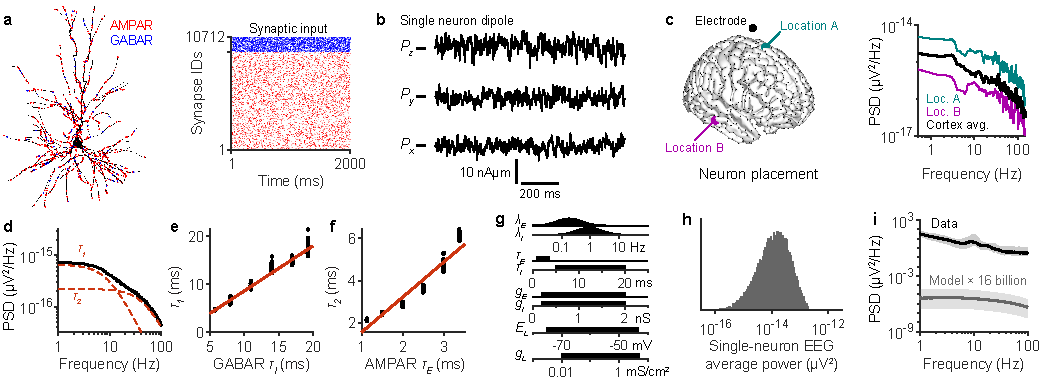
\includegraphics[width=177mm]{Figures/chapter2/figure1.pdf}}

    \centerline{
    \begin{minipage}[c]{177mm}
    \caption{\captiontitle{EEG cannot reflect asynchronous neural activity.} \textbf{a} Example morphology of a layer 2/3 pyramidal neuron. Inputs at AMPAR (red) and GABAR (blue) synapses were simulated with Poissonian spike trains, shown in raster plot. Only 1,000 synapses shown for clarity. Neuron morphology adapted from Budd, J. M. L. et al. Neocortical axon arbors trade-off material and conduction delay conservation. PLoS Comput. Biol. 6, e1000711 (2010). \textbf{b} The $x$, $y$, and $z$ components of the single-neuron dipole vector, calculated from (\textbf{a}). \textbf{c} Left: single-neuron EEG signals were simulated at the marked electrode location, with the neuron located at various source locations, e.g. location A and B. Right: the location-averaged EEG spectrum (black) computed by averaging over the source locations shown in black dots on the brain template. Loc.=location; Avg.=average. \textbf{d} Location-averaged spectrum generated from 1000 simulations of 11 representative neuron morphologies (\autoref{tab:tableS2.1}). The spectrum was fit by \ref{eq:linear_model} and the two Lorentzian components are shown in dashed red lines. \textbf{e} The unitary spectrum was calculated while varying the deactivation kinetics of GABARs ($\tau_I$) and the parameter $\tau_1$ was estimated. Red line has a slope of 1. \textbf{f} Same as (\textbf{e}), but showing $\tau_2$ as a function of the deactivation kinetics of AMPARs ($\tau_E$). \textbf{g} Sampling distributions for model parameters. $\lambda_E$, $\tau_E$, and $g_E$ represent the average input rate, the deactivation time constant, and maximal conductance for AMPAR synapses. $\lambda_I$, $\tau_I$, and $g_I$ represent the same parameters for GABAR synapses. $E_L$ and $g_L$ represent the reversal potential and conductance of the passive membrane leak current. \textbf{h} Distribution of single-neuron EEG power (location-averaged as in \textbf{c}) based on 20000 simulations with parameters sampled from the distributions shown in g and morphologies sampled as described in \autoref{tab:tableS2.1}. \textbf{i} Black: Median EEG spectrum across 14 subjects, with error bands indicating minimum and maximum spectral density. Grey: the predicted EEG spectrum of 16 billion uncorrelated neurons receiving Poissonian synaptic input (grey), with parameter values sampled from the distributions in (\textbf{a}). Error bands reflect 5 to 95\% quantile range.} 
    \label{fig:figure2.1}
    \end{minipage}
    }
\end{figure}

The unitary spectrum exhibited two important features. First, even with random synaptic input, the unitary spectrum displayed a trend. This trend could be described as the sum of two Lorentzian functions
\begin{equation} \label{eq:linear_model}
    S(f) = \frac{A_1}{1+(2\pi \tau_1 f)^2} + \frac{A_2}{1+(2\pi \tau_2 f)^2}
\end{equation}
as predicted by simple linear models of EEG generation \cite{Gao2017,Miller2009} (\autoref{fig:figure2.1}d). The slower ($\tau_1$) and faster ($\tau_2$) timescales were governed by the deactivation kinetics of GABA receptors (GABARs) and AMPA receptors (AMPARs), respectively (\autoref{fig:figure2.1}e, f). These simulations validate previous predictions that the relative contribution of excitatory and inhibitory currents to the EEG signal fundamentally affects the spectral trend \cite{Gao2017}.

Second, the unitary spectrum reflects the amplitude with which an average neuron contributes to the EEG signal. To investigate this idea in more detail, we examined the effect of varying all the model parameters within physiologically reasonable ranges (\autoref{fig:figure2.1}g). Measuring the average power of the resulting single-neuron EEGs revealed a range of possible amplitudes for the contribution of individual neurons to the EEG signal (\autoref{fig:figure2.1}h). These simulations show that no physiologically plausible parameters could allow 16 billion uncorrelated neurons to generate detectable EEG signals (\autoref{fig:figure2.1}i). More importantly, these calculations quantify how far off a completely asynchronous cortex is from generating detectable EEG signals. These calculations account for the EEG strength contributed by synaptic current amplitudes, neuron geometry, average firing rate of neurons, the number of neurons, the conductivity of various tissues, and the geometry of the cortex. Therefore, this result indicates that neural dynamics are responsible for the approximate four orders of magnitude difference between the simulated asynchronous spectrum and real EEG recordings.

\subsection{Detectable EEG requires only weak, locally synchronized dipoles}

\begin{wrapfigure}[20]{r}{80mm}
\vspace{-12pt}
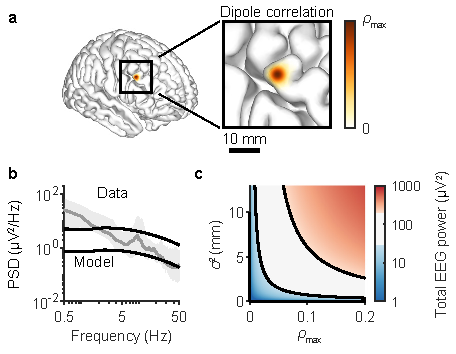
\includegraphics[width=77mm]{Figures/chapter2/figure2.pdf}
\vspace{-10pt}
    \caption{ \captiontitle{Detectable EEG signals require only weak, locally synchronized dipoles.}
	\textbf{a} Schematic displaying the coupling kernel used to correlate single-neuron dipoles. The kernel is a Gaussian function with peak of $\rho_{max}$ and variance $\sigma^2$.
	\textbf{b} Median EEG spectrum across 14 human subjects (grey; same error bands as \autoref{fig:figure2.1}i), and simulated unitary spectrum (black; same as \autoref{fig:figure2.1}d) scaled by arbitrary amounts to determine a lower and upper bound of the spectral trend amplitude. 
	\textbf{c} Heatmap of the total simulated EEG power produced by 16 billion neurons with dipoles coupled with the kernel in (\textbf{a}), and parameterized with various values of $\rho_{max}$ and $\sigma^2$. The black lines are level curves representing the lower and upper bounds for the spectral trend magnitude obtained in (\textbf{b}).
    } \label{fig:figure2.2}
\end{wrapfigure}

If the amplitude of EEG signals precludes asynchronous activity from shaping EEG spectra, what types of arrhythmic activity could influence EEG signals? To begin addressing this question, we first quantified in general how much dipole correlation is required to generate detectable EEG signals. To do so, we imposed a simplified spatial organization on a cortical template whereby neighbouring neurons produced correlated dipoles. Specifically, the dipoles of neurons separated by $d$ \unit{\milli\meter} were correlated with a coefficient of $\rho(d)=\rho_{max}\exp{(-d^2/\sigma^2)}$, where $\rho_{max}$ is the maximal dipole correlation and $\sigma^2$ is the spatial scale over which correlations decline (\autoref{fig:figure2.2}a). Based on this correlation scheme, the geometry of the cortex, average densities of neurons, and the single-neuron EEG amplitudes from the previous section, we estimated the power of the ensemble EEG signal that would be produced with different values of $\rho_{max}$ and $\sigma^2$ (see Methods). To capture the EEG spectral trend, we estimated that broadband EEG signals need to have a total power of between 50 and 200 \unit{\micro\volt\squared} (\autoref{fig:figure2.2}b). Thus for neural activity to generate detectable EEG signals, this activity needs to be capable of driving single-neuron dipoles that are correlated up to a value ($\rho_{max}$) of 0.06 to 0.12 (\autoref{fig:figure2.1}c), assuming a liberal range for $\sigma^2$ of 5-13 \unit{\milli\meter} (\autoref{fig:figure2.1}c; see Methods). While the existence of EEG rhythms prove that neural oscillations can generate the requisite dipole synchrony, it remains to be determined if and how such a degree of dipole coherence may be achieved by arrhythmic neural activity. 


% \begin{figure}
%   \begin{minipage}[c]{77mm}
%     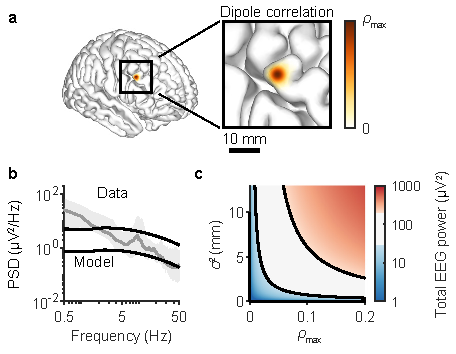
\includegraphics[width=\textwidth]{Figures/chapter2/figure2.pdf}
%   \end{minipage}\hfill
%   \begin{minipage}[c]{77mm}
%     \caption{ \captiontitle{Detectable EEG signals require only weak, locally synchronized dipoles.}
% 	\textbf{a} Schematic displaying the coupling kernel used to correlate single-neuron dipoles. The kernel is a Gaussian function with peak of $\rho_{max}$ and variance $\sigma^2$.
% 	\textbf{b} Median EEG spectrum across 14 human subjects (grey; same error bands as \autoref{fig:figure2.1}i), and simulated unitary spectrum (black; same as \autoref{fig:figure2.1}d) scaled by arbitrary amounts to determine a lower and upper bound of the spectral trend amplitude. 
% 	\textbf{c} Heatmap of the total simulated EEG power produced by 16 billion neurons with dipoles coupled with the kernel in (\textbf{a}), and parameterized with various values of $\rho_{max}$ and $\sigma^2$. The black lines are level curves representing the lower and upper bounds for the spectral trend magnitude obtained in (\textbf{b}).
%     } \label{fig:figure2.2}
%   \end{minipage}
% \end{figure}

\begin{figure}[b!]
    \centering
    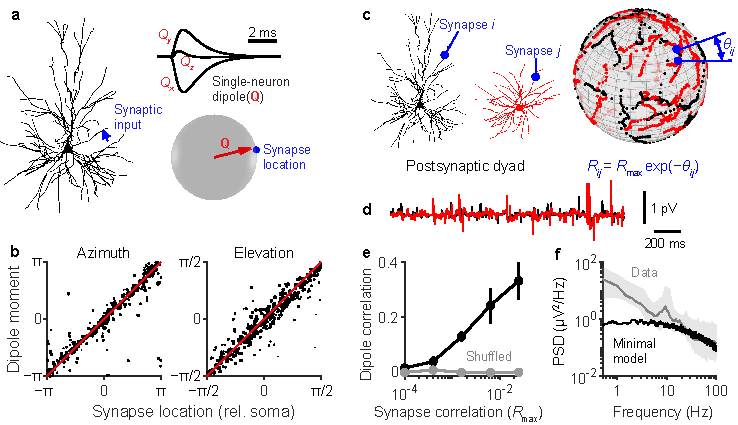
\includegraphics[width=125mm]{Figures/chapter2/figure3.pdf}
    \caption{\captiontitle{A minimal model of dipole correlation captures broadband EEG amplitude but not low frequency power.}
	\textbf{a} A single synapse was activated at the location specified by the blue arrow, generating a response in the single-neuron dipole, Q. The dipole vector at the peak of the response is oriented towards the synapse location, defined in spherical coordinates with the soma as the origin. Neuron morphology adapted from Budd, J. M. L. et al. Neocortical axon arbors trade-off material and conduction delay conservation. PLoS Comput. Biol. 6, e1000711 (2010).
	\textbf{b} The simulation in (\textbf{a}) was repeated 600 times with different neuron morphologies and synapse locations. Plotting the dipole orientation at the peak of the response against the location of the stimulated synapse shows a strong, linear relationship. Some points not plotted for clarity. Dot size is proportional to peak dipole amplitude. rel.=relative. 
	\textbf{c} Schematic showing the minimal model for dipole correlation. Synapses on each postsynaptic neuron in the dyad were projected onto a sphere. A correlation matrix among all synapses was then defined such that synapses separated by an angle $\theta_{ij}$ on the sphere were correlated by $R_{max}\exp{(-\theta_{Ij})}$. The left neuron’s morphology is adapted from Budd, J. M. L. et al. Neocortical axon arbors trade-off material and conduction delay conservation. PLoS Comput. Biol. 6, e1000711 (2010). The illustration of the right neuron is adapted, with permission from SNCSC, from Mainen, Z. F. \& Sejnowski, T. J. Influence of dendritic structure on firing pattern in model neocortical neurons. Nature 382, 363–366 (1996), Springer Nature.
	\textbf{d} Example of single-neuron EEG signals of the two neurons shown in (\textbf{c}).
	\textbf{e} Correlation between two single-neuron dipoles as a function of $R_{max}$. Vertical lines represent 95\% confidence intervals of the mean ($n=11$ different morphology pairs). When synapse locations are shuffled, dipoles are no longer correlated (grey).
	\textbf{f} The unitary spectrum of neurons receiving input calculated with the minimal model (black), scaled to compare the shape of the spectrum with median EEG spectrum of 14 subjects (grey line; same as \autoref{fig:figure2.1}i).} 
    \label{fig:figure2.3}
\end{figure}

\subsection{Synapse topology is sufficient for dipole correlations}
To investigate the ability of neural activity to generate coherent dipoles, we simulated dyads of neurons and investigated the level of correlation achievable between the two single-neuron dipoles. In our simulations, we noticed that if a single synapse was activated, the orientation of the resulting dipole could be accurately predicted by the orientation of the synapse relative to the soma (\autoref{fig:figure2.3}a, b). This result held across all neuron morphologies investigated (\autoref{fig:figureS2.1}). From this observation, we devised a minimal model of dipole coherence. To generate synaptic input, we projected the synapses of two neurons onto a sphere and correlated the inputs of synapses with close angular distances (\autoref{fig:figure2.3}c). By changing the maximal correlation between synapses, dipole correlation between neurons of various morphologies could be tuned continuously between 0 and ${\sim}0.3$ (\autoref{fig:figure2.3}d, e). Shuffling the location of the synapses abolished any dipole correlation (\autoref{fig:figure2.3}d). These results demonstrate that to generate detectable EEG signals, it is necessary and sufficient for synaptic input to exhibit temporal and spatial correlation. These conditions do not by themselves preclude any specific type of neural dynamics. Indeed this minimal model relied on independently sampled spikes at every time point and thus generated EEG signals with no temporal autocorrelation and a spectrum with the same shape as the asynchronous unitary spectrum (\autoref{fig:figure2.3}f). Therefore, the plausibility of aperiodic EEG signals depends solely on the ability for a network of neurons to generate arrhythmic activity with the requisite levels of spatiotemporal correlation. 

\subsection{Subcritical networks can generate aperiodic EEG signals}
We next investigated network models that could generate detectable, aperiodic EEG signals. To determine whether network activity could produce coherent dipoles, we utilized the results from the previous section (\autoref{fig:figure2.3}). After simulating a presynaptic neuron population, we used the UMAP algorithm\cite{McInnes2018} to embed the population onto a sphere in such a way that minimized the distance between presynaptic neurons with correlated spiking activity (\autoref{fig:figure2.4}a). These presynaptic neurons were then projected onto the dendrites of the postsynaptic dyad (\autoref{fig:figure2.4}a). By construction, synapses with higher correlations should have smaller angular distances, thus optimizing for dipole coherence. Effectively, this procedure tests whether it is geometrically possible for a network to generate sufficiently coherent synaptic input for EEG generation. 


\begin{figure}[t!]
    \centering
    \centerline{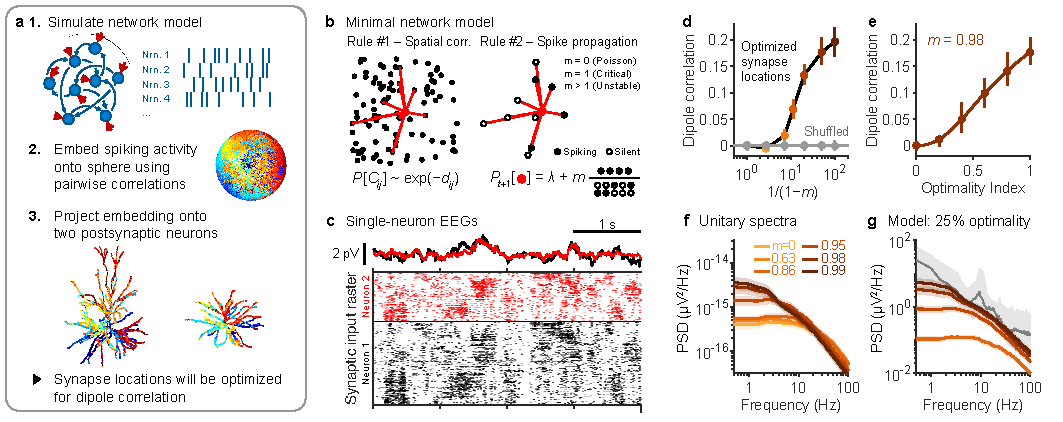
\includegraphics[width=180mm]{Figures/chapter2/figure4.pdf}}

    \centerline{
    \begin{minipage}[c]{180mm}
    \caption{\captiontitle{Subcritical network dynamics can explain the amplitude and low frequency power of broadband EEG.}
	\textbf{a}~Illustration of the algorithm for optimizing dipole coherence. Nrn. = neuron. The left neuron morphology is adapted from Budd, J. M. L. et al. Neocortical axon arbors trade-off material and conduction delay conservation. PLoS Comput. Biol. 6, e1000711 (2010). The illustration of the right neuron is adapted, with permission from SNCSC, from Mainen, Z. F. \& Sejnowski, T. J. Influence of dendritic structure on firing pattern in model neocortical neurons. Nature 382, 363–366 (1996), Springer Nature.
	\textbf{b} Illustration of the rules used to produce spatiotemporal synchrony in a presynaptic network. Rule \#1: network topology is enforced by making the probability of pairwise connections, $P(C_{ij})$, decrease exponentially with distance, $d_{ij}$. Rule \#2: the probability of a neuron firing, $P_{t+1}$, depends on a baseline firing rate of $\lambda=\lambda_0(1-m)$ plus the average activity of its neighbours scaled by $m$. $\lambda_0$ is a predefined average firing rate; $m$ is the branching number of the network. corr.=correlation.
	\textbf{c} Examples of single-neuron EEG signals of two neurons receiving input from the network model with a branching number $m=0.98$, when synapse locations have been optimized as described in (\textbf{a}). Bottom: a raster plot of synaptic input for the two neurons. 
	\textbf{d} Correlation between two single-neuron dipoles as a function of the branching number, m, of the presynaptic network. Dipole correlation increases with $m$ (coloured dots), but not when synapse locations are shuffled (grey).  Median (dots) and 5 to 95\% quantile range (vertical lines) across $n=10000$ simulated dyads with randomly sampled morphologies (\autoref{tab:tableS2.1}) and randomly sampled biophysical parameter values (as in \autoref{fig:figure2.1}g).
	\textbf{e} Dipole correlation can be tuned by placing synapses suboptimally (see Methods). Cubic interpolation between simulated optimality indices is shown with the solid line. Median (dots) and 5 to 95\% quantile range (vertical lines) across n=500 simulations.
	\textbf{f} Unitary spectra calculated for different branching numbers. Error bands reflect 95\% confidence interval of the mean.
	\textbf{g} The unitary spectra from (\textbf{f}) scaled based on a synapse optimality index of 0.25 (colours same as in \textbf{f}). The value of $\rho_{max}$ was determined from (\textbf{e}) and the final scaling factor was determined as in \autoref{fig:figure2.2}. Grey: median EEG spectrum of 14 subjects (same as \autoref{fig:figure2.1}i).} 
    \label{fig:figure2.4}
    \end{minipage}
    }
\end{figure}


To understand the mechanisms of aperiodic EEG generation, we attempted to construct the simplest network that could generate dipole coherence. Our previous results demonstrate that randomly connected networks cannot generate coherent dipoles, because they cannot produce spatially correlated activity. We therefore continued on to use the simplest neural network that exhibits spatial topology, namely, a spatial network. To construct the network, each neuron was embedded in a plane and connected preferentially to nearby neurons (\autoref{fig:figure2.4}b). For simplicity, we modelled individual neurons as binary nodes, i.e., each neuron was either spiking or quiescent. Spikes propagated along network connections, causing subsequent neurons to fire with some probability (\autoref{fig:figure2.4}b). This simple model falls within the category of a branching network, because the dynamics are governed by a single parameter called the branching number, denoted by m, which reflects the average number of spikes successfully elicited across the network when a single neuron fires. 

Our simulations revealed that the maximal achievable dipole correlation increased with the network’s branching number (\autoref{fig:figure2.4}c, d). A purely asynchronous network ($m=0$) was unsurprisingly incapable of generating correlations among single-neuron dipoles (\autoref{fig:figure2.4}d). On the other hand, a slightly subcritical network ($m=0.98$) was capable of generating dipoles that were correlated by $0.18 \pm 0.001$ for an average pair of postsynaptic neurons (mean $\pm$ SE, $n=10000$; morphologies sampled as described in \autoref{tab:tableS2.1}; biophysical parameters sampled as in \autoref{fig:figure2.1}g). This branching number is significant because previous work has found that networks with a branching number of $m=0.98$ closely reproduced the in vivo dynamics of cortical spiking across many different species \cite{Suryadi2022, Wilting2019}, making this a physiologically plausible parameter value. Placing synapses suboptimality led to proportionally lower dipole correlation, revealing that subcritical dynamics can still drive coherent dipoles with suboptimal synapse placement (\autoref{fig:figure2.4}e). Based on the amplitude of the computed unitary spectrum (\autoref{fig:figure2.4}f), we estimated that subcritical network activity can produce realistic EEG amplitudes with synapse optimality as low as ${\sim}25$\% (\autoref{fig:figure2.4}g; see Methods). As a reference, an optimality index of 50\% means that strongly correlated synapses will on average lie on the same hemisphere of their respective neurons, a geometry reminiscent of the apical-basal compartmentalization of cortical pyramidal neurons. 

Notably, stronger dipole correlations coincided with longer temporal autocorrelations in network activity (\autoref{fig:figure2.4}f), a phenomenon directly resulting from the causality of spike propagation (\autoref{fig:figure2.4}b). This means that EEG signals produced by propagating cortical spikes must have higher power at low frequencies if the signals are to be of detectable amplitudes. This result illustrates a fundamental constraint that may in part explain the 1/f scaling of EEG spectra at lower frequencies (\autoref{fig:figure2.4}g). More broadly, these results demonstrate a biophysically feasible mechanisms that allows arrhythmic neural activity to generate EEG signals, and to consequently influence the broadband features of EEG spectra.

\subsection{Narrowband EEG changes could result from arrhythmic activity}
The above calculations show that arrhythmic neural activity can in theory generate broadband EEG signals, meaning that narrowband EEG power need not reflect brain rhythms. We therefore asked whether EEG signals that are produced by arrhythmic activity can confound traditional EEG interpretation, namely, that changes in bandpower reflect differences in neural oscillations. To address this question, we considered a scenario where the EEG signal is generated by two subpopulations of neurons: a population exhibiting synchronous oscillations, and a second population exhibiting subcritical dynamics ($m=0.98$). If these population are completely independent of one another, their EEG contributions will by definition add together linearly. To investigate further, we simulated the scenario in which the two populations’ postsynaptic signals are intermixed (\autoref{fig:figure2.5}a). One interpretation of this setup could be a cortical neuron that is receiving oscillatory input from, say, the thalamus, while also receiving subcritical input from the local cortical circuitry. Compared to neurons receiving entirely oscillatory input or entirely subcritical input, the neuron receiving mixed input produced a unitary EEG spectrum that exhibited a mixed phenotype (\autoref{fig:figure2.5}b). Increasing the strength of the oscillatory and/or aperiodic input altered the amplitude of the spectral peak and/or spectral trend (\autoref{fig:figure2.5}c-e). However, changes to the spectral trend did not multiplicatively scale the oscillatory peak amplitude. As a result, quantifying the amplitude of oscillatory peaks relative to the spectral trend produced incorrect interpretations (\autoref{fig:figure2.5}f-h): dividing the peak amplitude by the background trend erroneously suggested that the neural rhythm decreased when aperiodic activity became stronger (\autoref{fig:figure2.5}d, g), and severely underestimated the neural rhythm increase when aperiodic activity increased concomitantly (\autoref{fig:figure2.5}e, h). We therefore concluded that if a spectral peak is clearly discernible, then arrhythmic neural activity has a minimal confounding influence and detrending is unnecessary. Importantly, however, if no spectral peak is obvious, then there is no guarantee that changes in power result from differences in neural oscillations.

\begin{figure}[t!]
    \centering
    \centerline{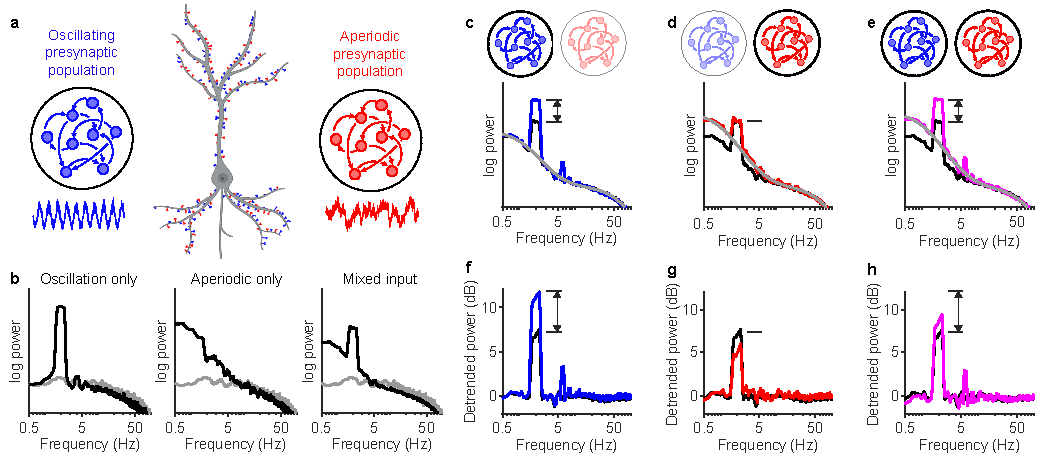
\includegraphics[width=176mm]{Figures/chapter2/figure5.pdf}}

    \centerline{
    \begin{minipage}[c]{176mm}
\caption{\captiontitle{Measuring oscillatory peak power relative to spectral trend may produce misleading results.}
	\textbf{a} Illustration of mixed input model. Half of the neuron’s synapses received oscillatory rhythmic input (blue) and the other half received input from a subcritical network (red). The strengths of oscillatory and subcritical dynamics were adjusted by tuning two parameters, $\alpha_R$ and $\alpha_A$, respectively, which determined the degree to which synaptic inputs differed from homogenous Poisson processes. See Methods for details. Neuron illustration created with BioRender.com.
	\textbf{b} Unitary spectrum for neurons receiving Poisson input (grey), compared with the unitary spectra for neurons receiving input entirely from the oscillatory population (left; black), entirely from the subcritical population (middle; black), or mixed input as in a (right; black): $\alpha_R=\alpha_A=0.1$.
	\textbf{c} Oscillatory input was strengthened by increasing $\alpha_R$ from 0.1 (black) to 0.5 (blue), with $\alpha_A$ fixed at 0.1. The spectra were fit using a FOOOF-like algorithm\cite{Donoghue2020}, except that here the aperiodic component was modelled with \ref{eq:linear_model} (solid grey line).
	\textbf{d} Aperiodic input was strengthened by increasing $\alpha_A$ from 0.1 (black) to 0.5 (red), with $\alpha_R$ fixed at 0.1.
	\textbf{e} Both oscillatory and aperiodic inputs were strengthened by increasing both $\alpha_R$ and $\alpha_A$ from 0.1 (black) to 0.5 (magenta).
	\textbf{f} Detrended spectrum of neurons receiving mixed input before (black) and after (blue) oscillation strength increased. The unitary spectra in (\textbf{c}) were divided by the solid grey line. 
	\textbf{g} Detrended power before (black) and after (red) aperiodic strength increases. Notice that the detrended power at \qty{2}{\hertz} decreases, despite the strength of oscillations remaining the same.
        \textbf{h} Detrended power before (black) and after (magenta) both oscillation and aperiodic strength increases. Notice that the detrended power at \qty{2}{\hertz} does not increase as much as in (\textbf{f}), despite the oscillation increasing in strength by the same amount.} 
    \label{fig:figure2.5}
    \end{minipage}
    }
  
    
\end{figure}


\subsection{Spectral slope is an inconsistent measure of EI balance}
The above results focused on the role of neural dynamics in shaping the EEG spectrum. However, \autoref{fig:figure2.1}d-f show that the kinetics of postsynaptic responses also impact the broadband properties of EEG spectra. To further investigate this mechanism shaping EEG spectra, we performed a full sensitivity analysis of the spectral slope with respect to the biophysical parameters in the single-neuron models. The unitary EEG spectrum was simulated with many different parameter values (\autoref{fig:figure2.6}a) and the overall slope of the spectrum was calculated \cite{Donoghue2020} between 1 and 40 \unit{\hertz} (\autoref{fig:figure2.6}b). These simulations revealed that the spectral slope was consistently affected by four parameters: $\tau_I$, $g_E$, $g_I$, and $E_L$ (\autoref{fig:figure2.6}c). These results can be explained through \ref{eq:linear_model}. The parameter $\tau_I$ directly determines the slow timescale, $\tau_1$, of the unitary spectrum (\autoref{fig:figure2.1}d), whereas synaptic conductances, $g_E$ and $g_I$, directly govern the contributions of inhibitory and excitatory synaptic currents, respectively. The reversal potential, $E_L$, of the leak current alters the spectral slope because when $E_L$ is more depolarized, GABA\textsubscript{A} receptors experience a higher driving force, thus amplifying the contributions of inhibitory currents. 


\begin{wrapfigure}[20]{r}{90mm}
\vspace{-12pt}
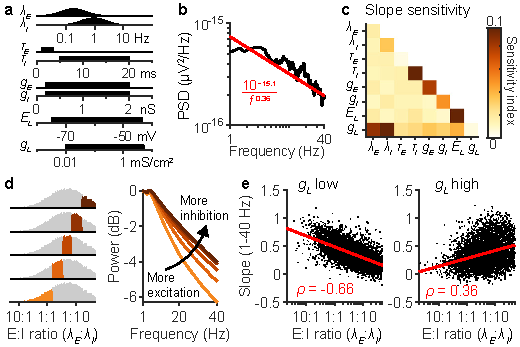
\includegraphics[width=90mm]{Figures/chapter2/figure6.pdf}
\vspace{-22pt}
    \caption{
       \captiontitle{Sensitivity of spectral slope to biophysical parameters governing postsynaptic responses.}
	\textbf{a} Sampling distributions for model parameters, the same as the ones used in \autoref{fig:figure2.1}g.
	\textbf{b} Example single-neuron EEG spectrum, fitted with the equation ${10}^\alpha/f^\beta$ between 1 and \qty{40}{\hertz}.
	\textbf{c} Sensitivity of the spectral slope, $\beta$, to model parameters, with first and second order interactions, calculated from 20000 simulated spectra.
	\textbf{d} Simulated spectra were averaged depending on the ratio between $\lambda_E$ and $\lambda_I$. Lower E:I ratios correspond to more inhibition.
	\textbf{e} The spectral slope is plotted against the E:I ratio for each simulation. Left: simulation where the leak conductance was low ($g_L<0.1$ \unit{\milli\siemens\per\centi\meter\squared}; $n=7366$ simulations). Right: simulation where the leak conductance was high ($g_L>1$ \unit{\milli\siemens\per\centi\meter\squared}; $n=5184$ simulations).
    } \label{fig:figure2.6}
\end{wrapfigure}

% \begin{figure}
%   \begin{minipage}[c]{90mm}
%     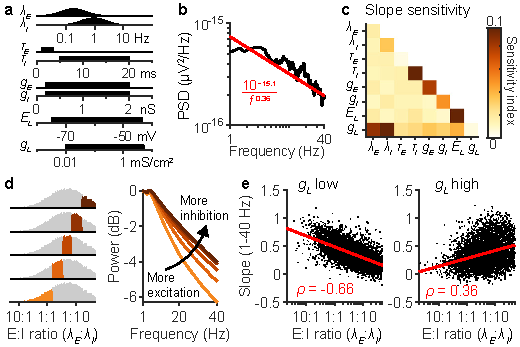
\includegraphics[width=\textwidth]{Figures/chapter2/figure6.pdf}
%   \end{minipage}\hfill
%   \begin{minipage}[c]{70mm}
%     \caption{
%        \captiontitle{Sensitivity of spectral slope to biophysical parameters governing postsynaptic responses.}
% 	\textbf{a} Sampling distributions for model parameters, the same as the ones used in \autoref{fig:figure2.1}g.
% 	\textbf{b} Example single-neuron EEG spectrum, fitted with the equation ${10}^\alpha/f^\beta$ between 1 and \qty{40}{\hertz}.
% 	\textbf{c} Sensitivity of the spectral slope, $\beta$, to model parameters, with first and second order interactions, calculated from 20000 simulated spectra.
% 	\textbf{d} Simulated spectra were averaged depending on the ratio between $\lambda_E$ and $\lambda_I$. Lower E:I ratios correspond to more inhibition.
% 	\textbf{e} The spectral slope is plotted against the E:I ratio for each simulation. Left: simulation where the leak conductance was low ($g_L<0.1$ \unit{\milli\siemens\per\centi\meter\squared}; $n=7366$ simulations). Right: simulation where the leak conductance was high ($g_L>1$ \unit{\milli\siemens\per\centi\meter\squared}; $n=5184$ simulations).
%     } \label{fig:figure2.6}
%   \end{minipage}
% \end{figure}

Surprisingly, the analysis of the spectral slope revealed a strong interaction between $g_L$ and both $\lambda_E$ and $\lambda_I$ (\autoref{fig:figure2.6}c). When the leak conductance was low ($g_L<0.1$ \unit{\milli\siemens\per\centi\meter\squared}), the spectral slope was found to be negatively correlated with the $\lambda_E$:$\lambda_I$ ratio (\autoref{fig:figure2.6}d, e; \autoref{fig:figureS2.2}b), which contradicts the predictions of linear models of EEG generation \cite{Gao2017}. The reason is that when the leak conductance was low, higher E:I ratios drove the average membrane potential close to the reversal potentials of GABA receptors (\autoref{fig:figureS2.2}a). This caused neurons with low $g_L$ to experience vanishing GABAR driving forces and amplified AMPAR driving forces at high E:I values, consequently and counterintuitively making the spectral slope anticorrelated with the E:I ratio (\autoref{fig:figure2.6}e). However, when the leak conductance was high ($g_L>1$ \unit{\milli\siemens\per\centi\meter\squared}), the membrane potential fluctuated less and stayed within a relatively linear regime (\autoref{fig:figureS2.2}a). Consequently the spectral slope was positively correlated with E:I ratio (\autoref{fig:figure2.6}e) as predicted by linear models of EEG generation \cite{Gao2017}. A similar albeit weaker effect was observed in the relationship between the spectral slope and the $g_E$:$g_I$ ratio (\autoref{fig:figureS2.2}c). Generally, we conclude that the overall spectral trend is significantly affected by biophysical parameters that alter postsynaptic responses, but changes in the slope value do not alone inform what parameters are changing.

\subsection{Changes to synaptic responses confound brain rhythm quantification}
Differences in postsynaptic responses alter EEG spectra in a fundamentally different way to arrhythmic neural activity. Postsynaptic kinetics effectively interact as a convolution with synaptic input and should therefore interact with oscillatory peaks in a multiplicative manner. Moreover, postsynaptic mechanisms should affect power generated by all types of neural dynamics equally. To test this, we systematically altered the biophysical parameters that govern postsynaptic currents and analyzed the unitary spectra generated by various types of synaptic inputs, including white noise (\autoref{fig:figureS2.3}), subcritical dynamics (\autoref{fig:figure2.7}a), as well as three types of dynamics that exhibit spectral peaks: a recently proposed recurrent Ising model that exhibits co-existence of oscillations and avalanches\cite{Lombardi2023} (\autoref{fig:figureS2.3}), an underdamped second-order system driven by white noise (\autoref{fig:figureS2.3}), and finally a simple sinusoidal rhythm (\autoref{fig:figure2.7}b). We investigated the effects of neurophysiological parameters that affect the spectral slope, as identified by our sensitivity analysis (\autoref{fig:figure2.6}c): GABAR kinetics ($\tau_I$), the leak current reversal potential ($E_L$), and the conductances of excitatory ($g_E$) and inhibitory ($g_I$) synapses. Changing these parameters altered the unitary spectra in distinct manners, but importantly had identical effects across the different types of the input dynamics (\autoref{fig:figure2.7}a, b; \autoref{fig:figureS2.3}). 


\begin{figure}
  \begin{minipage}[c]{90mm}
    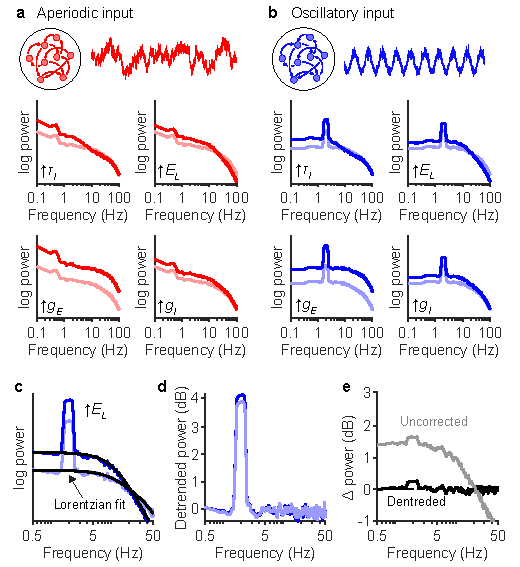
\includegraphics[width=\textwidth]{Figures/chapter2/figure7.pdf}
  \end{minipage}\hfill
  \begin{minipage}[c]{70mm}
    \vspace*{0.25cm}
    \caption{
       \captiontitle{Changes in postsynaptic mechanisms confound brain rhythm quantification.}
	\textbf{a} Unitary spectra for neurons receiving entirely subcritical input ($m=0.98$,$\alpha_A=0.1$; see \autoref{fig:figure2.5}a), before and after four parameter changes: subplot corresponding to ($\uparrow\tau_I$) shows the unitary spectrum when $\tau_I$  was increased from \qty{10}{\milli\second} (pink) to \qty{30}{\milli\second} (red); $(\uparrow E_L$) shows unitary spectrum when $E_L$ was increased from \qty{-60}{\milli\volt} (pink) to \qty{-45}{\milli\volt} (red); ($\uparrow g_E$) shows unitary spectrum when $g_E$ was increased from \qty{0.7}{\nano\siemens} (pink) to \qty{1.4}{\nano\siemens} (red); and ($\uparrow g_I$) shows unitary spectrum when $g_I$ was increased from\qty{0.7}{\nano\siemens} (pink) to \qty{1.4}{\nano\siemens} (red). Note the changes in the unitary spectra despite there being no changes in synaptic input dynamics.
	\textbf{b} Same as in (\textbf{a}), but for neurons receiving entirely oscillatory input ($\alpha_R=0.1$; see \autoref{fig:figure2.5}a). In \autoref{fig:figureS2.3}, we show examples of different types of rhythmic input.
	\textbf{c} Example of fitted spectral trend. Here, the unitary spectrum of sinusoidal input is shown before and after increasing $E_L$. The spectra were fit using a FOOOF-like algorithm\cite{Donoghue2020}, except that here the trend was modelled using \ref{eq:linear_model} (black lines). See other examples in \autoref{fig:figureS2.4}.
        \textbf{d} Spectra from (\textbf{c}), detrended by dividing the spectra by their respective Lorentzian fits. See other examples in \autoref{fig:figureS2.4}. 
    } \label{fig:figure2.7}
  \end{minipage}
  \begin{minipage}[c]{\textwidth}
    \vspace*{-0.72cm} \footnotesize \singlespacing
	\textbf{e} Change in EEG spectral density caused by increasing $E_L$. In grey is the raw change in the unitary spectra, while in black is the difference between the detrended spectra. Detrending the spectra with \ref{eq:linear_model} has corrected for the effects of increasing $E_L$ and correctly indicates that there are no changes in neural dynamics. 
  \end{minipage}
\end{figure}

The spectral changes caused by altering biophysical parameters do not reflect differences in neural dynamics and therefore represent confounds for EEG analysis. To correct for the effects of these parameter changes, we fit the part of the spectral trend produced by synaptic timescales using a FOOOF-like algorithm \cite{Donoghue2020}, except that the background trend was modelled using \ref{eq:linear_model} (\autoref{fig:figure2.7}c; \autoref{fig:figureS2.4}). As anticipated, detrending the spectra in this way corrected for the confounding effects of the parameter changes (\autoref{fig:figure2.7}d, e; \autoref{fig:figureS2.4}).

In conclusion, our modelling results indicate that there are two distinct mechanisms of peak-trend interaction in EEG spectra. In one case, there are changes in the relative contribution of rhythmic and arrhythmic neural activity to the EEG signal. In this case, the peaks and spectral trend change relatively independently from one another, and thus detrending is unnecessary for quantifying spectral peak amplitudes (see Discussion). In the other case, changes in biophysical parameters alter the mechanism of EEG generation itself. In this case, EEG differences are unrelated to neural dynamics; these changes can confound EEG signals from all neural sources, and thus even spectral peak amplitudes can be potentially corrupted.

\begin{figure}[b!]
    \centerline{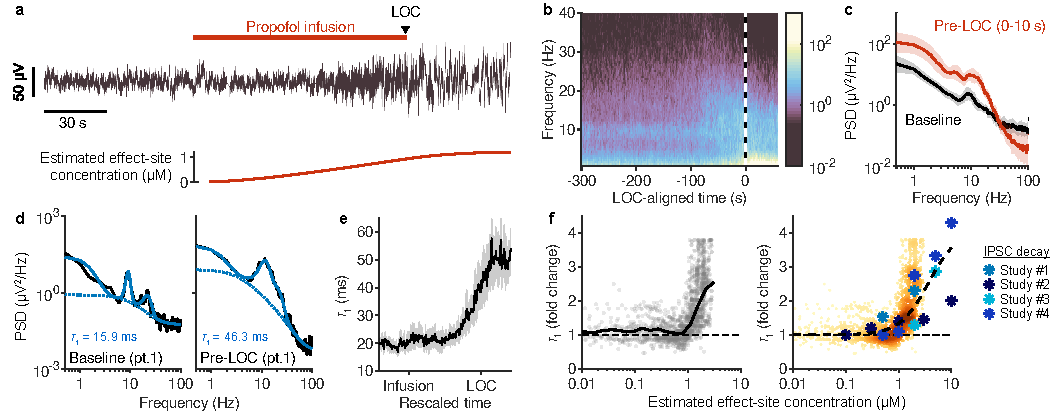
\includegraphics[width=180mm]{Figures/chapter2/figure8.pdf}}
    \centerline{
    \begin{minipage}[c]{180mm}
    \caption{\captiontitle{Model predicts and quantifies effects of propofol administration on EEG spectra.}
	\textbf{a} Representative EEG signal, Cz recording site, of a subject receiving an infusion of propofol until loss of consciousness (LOC). The estimated effect-site concentration of propofol is plotted below. 
	\textbf{b} Mean LOC-aligned spectrogram of 14 subjects. 
	\textbf{c} Average power spectrum at baseline (black), averaged between 0-10 \unit{\second} prior to propofol infusion, and after propofol infusion (red), averaged between 0-10 \unit{\second} prior to LOC. Shading reflects 95\% confidence intervals of the mean (n=14 subjects). 
	\textbf{d} Representative EEG spectrum at baseline, 0-10 \unit{\second} prior to propofol infusion (left, black) and 0-10 \unit{\second} prior to LOC (right, black). Spectra have been fitted with \ref{eq:fitting} (see Methods), using a FOOOF-like fitting algorithm\cite{Donoghue2020} that accounts for several Gaussian peaks in the spectra (solid blue). Fitted trend is shown with dashed line.
	\textbf{e} The parameter $\tau_1$, estimated from fits to spectra computed in 2-s windows, plotted with respect to rescaled time. Shading reflects 95\% confidence intervals of the mean (n=14 subjects).
	\textbf{f} Left: fold change in the estimated value of $\tau_1$ plotted against the estimated effect-site concentration of propofol. Black line marks the mean for each concentration of propofol. Right: The estimated dose-response plot from the left panel (darker colours reflect higher density of points) is superimposed with in vitro data taken from four studies: Study \#127, Study \#228, Study \#329, and Study \#429. The data values taken from these studies are presented in \autoref{tab:tableS2.2}. The dash black line is a fitted Hill function to the data from the four studies: $EC_{50} = 3.7$ \unit{\micro\molar} and Hill coefficient (n) = 1.6.} 
    \label{fig:figure2.8}
    \end{minipage}
    }
\end{figure}

\subsection{Model predicts and quantifies effects of propofol on EEG spectra}
The above results suggest that spectral detrending may be important in pharmacological experiments since many drugs target ion channels and alter postsynaptic responses. To test this model prediction, we investigated the EEG signatures of the general anesthetic propofol, a GABA\textsubscript{A} receptor modulator that lengthens the decay time of synaptic inhibition \cite{Franks2008, Kitamura2003, Orser1994, Whittington1996}. We recorded the EEG of 14 subjects during a fixed-rate infusion of propofol lasting until loss of consciousness (LOC) (\autoref{fig:figure2.8}a). The moment of LOC was identified by the dropping of a held object, which has been shown to provide an accurate, binary measure of LOC with precise timing \cite{Cummings1984,Guay2019}. The median LOC-aligned spectrogram was calculated from the Cz channel, which revealed an increase in low frequency power and a decrease in high frequency power starting before LOC (\autoref{fig:figure2.8}b). Comparing the average power spectrum at baseline (0-10 \unit{\second} prior to propofol infusion) to that following propofol infusion (0-10 \unit{\second} prior to LOC) revealed an increase in low frequency power and a decrease in high frequency power, thus giving the appearance of a rotation of the power spectrum (\autoref{fig:figure2.8}c). 

Our modelling results suggest that propofol inflates low frequency power by increasing the slow timescale, $\tau_1$, of the spectral trend (\autoref{fig:figure2.1}d, e; \autoref{fig:figure2.7}). To test this, we estimated $\tau_1$ from the EEG data by fitting a modified \ref{eq:linear_model} to the EEG spectra (\ref{eq:fitting}; see Methods). This modified function fit the spectral trend well except at frequencies less than ${\sim}3$ \unit{\hertz} (\autoref{fig:figure2.8}d; \autoref{fig:figureS2.5}a-c), where our modelling results suggest the spectral trend is coloured primarily by neural dynamics, such as delta oscillations and/or subcritical network activity, but not synaptic kinetics (\autoref{fig:figure2.4} \& \ref{fig:figure2.5}). Corroborating this interpretation, the low frequency ($<3$ \unit{\hertz}) part of the trend waxed and waned from second to second, occasionally disappearing entirely, whereas the fitted synaptic timescale remained stable between time windows (\autoref{fig:figureS2.5}c). The extracted timescale, $\tau_1$, was remarkably consistent prior to the infusion of propofol, with an average value of 16.7 ± 1.4 ms (mean $\pm$ SE, $n=14$) (\autoref{fig:figure2.8}e). Following the infusion of propofol, $\tau_1$ began increasing, reaching a value of 43.2 $\pm$ 4.6 \unit{\milli\second} ($p \approx 10^{-4}$; paired two-tailed t-test) 0-10 \unit{\second} prior to LOC (\autoref{fig:figure2.8}e). Similar changes were observed at other electrode sites (\autoref{fig:figureS2.6}). By plotting the estimated value of $\tau_1$ at each time point against the estimated effect-site concentration of propofol, quantified using the Marsh model \cite{Marsh1991}, we constructed a dose-response curve of fold change in $\tau_1$ against estimated propofol concentration (\autoref{fig:figure2.8}f). The inferred dose-response curve for $\tau_1$ quantitatively matched in vitro measurements of inhibitory postsynaptic current kinetics in the presence of bath applied propofol \cite{Kitamura2003, Orser1994, Whittington1996} (\autoref{fig:figure2.8}f). Thus, the changes in $\tau_1$ were consistent with expectations based on propofol’s known pharmacology. These observations support the model’s prediction that GABAR kinetics significantly shape EEG spectra and that broadband EEG changes do not necessarily reflect differences in brain dynamics. 


\subsection{Correcting for synaptic timescales reveals a unique signature of LOC}
Our modelling results predicted that propofol’s effect on synaptic timescales will produce errors in conventional quantifications of brain rhythms. Past studies have suggested that LOC from propofol is associated with changes in the delta (0.5-3 \unit{\hertz}), alpha (8-15 \unit{\hertz}), and beta (15-30 \unit{\hertz}) frequency ranges \cite{Purdon2013}. To investigate the consequences of spectral detrending on EEG signatures of LOC, we compared raw bandpower to detrended bandpower in the delta, alpha, and beta frequency ranges. To compare EEG dynamics across individuals, data were aligned simultaneously to the moment of propofol infusion and LOC; this was done by rescaling time in each experiment by the latency to LOC (median: 135 s; range: 95-285 s). Similar results were obtained when time was not rescaled (\autoref{fig:figureS2.5}d). Consistent with previous studies\cite{Purdon2013}, raw baseline-normalized power increased in the delta, alpha, and beta band following propofol infusion (\autoref{fig:figure2.9}a-c). Whereas alpha power increased quickly and plateaued prior to LOC, delta power rose slowly and continued increasing until after LOC (\autoref{fig:figure2.9}d). Notably, beta power increased concomitantly with alpha power, but then began decreasing prior to LOC, eventually producing a beta power not statistically different from baseline post-LOC (\autoref{fig:figure2.9}d). 




\begin{figure}[t!]
    \centerline{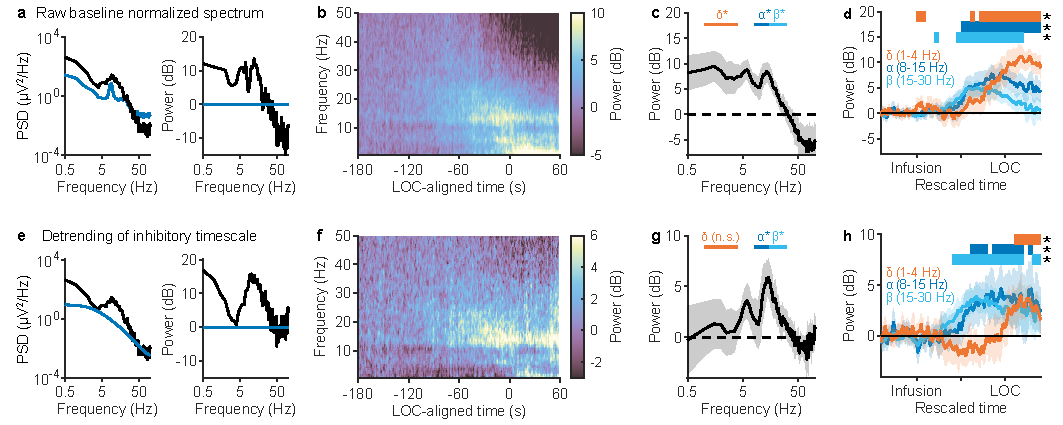
\includegraphics[width=180mm]{Figures/chapter2/figure9.pdf}}
    \centerline{
    \begin{minipage}[c]{180mm}
    \caption{\captiontitle{Correcting for synaptic timescales reveals a unique signature of losing consciousness.}
	\textbf{a} Left: representative EEG power spectrum following LOC (black) of a single subject, superimposed on the power spectrum at baseline (blue). Right: power spectrum following LOC (black) normalized to baseline. 
	\textbf{b} Mean baseline normalized spectrogram (n=14 subjects).
	\textbf{c} Average baseline-normalized power 0-10 \unit{\second} prior to LOC (shading: 95\% confidence interval of mean). Power was significantly elevated within the delta ($p=0.001$, right-tailed sign test; $n=14$ subjects), alpha ($p\approx10^{-4}$), and beta ($p=0.007$) frequency bands.
	\textbf{d} Changes in alpha, beta, and delta power, aligned to both moment of propofol infusion and LOC, averaged across subjects (shading: 95\% confidence interval of mean). Bars above graph indicate 0.05-long segments of rescaled time where there is a statistically significant increase ($p<0.05$, right-tailed sign test) in the corresponding frequency band power. \autoref{fig:figureS2.5}d shows results without rescaled time. 
	\textbf{e} Left: EEG spectrum following LOC, same as (\textbf{a}), superimposed with fitted inhibitory timescale (\ref{eq:fitting}). Fitted Gaussian peaks not shown. Right: detrended power, defined as power relative to fitted inhibitory timescale, in decibels. 
	\textbf{f} Mean detrended spectrogram, normalized to baseline (n=14 subjects).
	\textbf{g} Detrended power 0-10 \unit{\second} prior to LOC, normalized to baseline (shading: 95\% confidence interval of mean). Power was significantly elevated within the alpha ($p= 0.006$) and beta, ($p=0.001$), but not delta ($p=0.40$) frequency bands. Significance testing same as (\textbf{c}).
	\textbf{h} Same as in (\textbf{d}), but for detrended power, normalized to baseline.} 
    \label{fig:figure2.9}
    \end{minipage}
    }
\end{figure}
 

To correct for the confounding effects of propofol, we divided EEG power at each timepoint by the estimated synaptic timescales fitted from the previous section (\autoref{fig:figure2.9}e). We then normalized detrended power by the detrended power at baseline (\autoref{fig:figure2.9}f), such that changes in bandpower reflected the spectral changes unexplained by the increase in $\tau_1$. This procedure entirely removed the apparent rotation in the EEG spectra following propofol infusion (\autoref{fig:figure2.9}g). As a result of this detrending, power in the alpha, beta, and delta bands clearly increased at distinct times (\autoref{fig:figure2.9}h). Alpha and beta power appeared following propofol infusion and plateaued well before LOC. In contrast, detrended delta power did not increase until the moment of LOC, at which point it increased sharply (\autoref{fig:figure2.9}h; \autoref{fig:figureS2.5}d). In summary, whereas the raw EEG signal failed to exhibit a strongly time-locked signal at the moment of LOC, removing the anticipated confounds of propofol revealed a sharp increase in delta power within seconds of LOC. This analysis combined with our modelling results suggest that pharmacological changes to synaptic kinetics may mask the true dynamics of neural oscillations when spectral detrending is not performed. Additionally, these results point to distinct roles for alpha and delta power in the function of propofol as a general anesthetic. 

\section{Discussion}
In this study, we explored the neural basis of the EEG spectral trend and examined its implications for EEG interpretation and analysis. Several important conclusions came out of this investigation. First, this work provided biophysical evidence that arrhythmic neural activity is capable of generating detectable EEG signals. Second, our modelling consolidated the predictions of simpler computational models \cite{Gao2017, Chaudhuri2018} and indicated that the EEG spectral trend is shaped by the interactions of many factors, including synaptic kinetics, excitatory-inhibitory ratio, and aperiodic network dynamics. Third, our analysis revealed that spectral peak amplitudes are minimally affected by fluctuations in arrhythmic neural activity. On the other hand, we found that systemic changes in synaptic current properties do necessitate detrending to accurately interpret spectral changes as variations in neural activity. Our results suggested that this latter scenario is particularly important for EEG recordings used in tandem with pharmacological interventions. 

Traditional spectral analysis assumes that EEG power within canonical frequency bands reflect various brain rhythms. Our modelling results seriously challenge this assumption. Specifically, if a spectral peak is not evident within a given frequency band, our work justifies a physiologically plausible and biophysically realistic alternative hypothesis, namely, that the bandpower reflects broadband neural activity. Our results thus validate the principle assumption of spectral detrending methods, such as the FOOOF algorithm \cite{Donoghue2020}, which is that peak detection is a necessary prerequisite to quantifying oscillatory power. While power lying outside spectral peaks could potentially reflect neural rhythms, there is no theoretical guarantee for this interpretation based on spectral analysis alone. 

Importantly, our results do not necessarily support a purely data-driven approach to detrending EEG spectra. While changes in arrhythmic activity affect spectral peaks in an additive manner (\autoref{fig:figure2.5}), changes in synaptic currents multiplicatively scale spectral peaks (\autoref{fig:figure2.7}); these two mechanisms thus require two distinct methods of detrending, i.e., subtractive versus divisive detrending, respectively. Without prior knowledge, it is unclear which method is required. Moreover, given the amplitude of peaks above the background trend typical in EEG spectra, small additive changes in the trend would alter the peak amplitudes minimally compared to the errors introduced by incorrectly detrending (\autoref{fig:figure2.5}). Overall, we conclude that spectral detrending should not be performed unless there is clear physiological and biophysical justification and validation. 

In the analysis presented here, there was prior knowledge of the well-documented action of propofol on GABAR kinetics \cite{Kitamura2003, Orser1994, Whittington1996}, clearly indicating the necessity for divisive detrending. To mitigate the chances of overfitting, we constrained parameter values to physiologically reasonable ranges, and validated that the fitted spectral changes and $\tau_1$ values quantitatively matched expectations. Even so, our decomposition of spectra into physiologically distinct components was likely imperfect, especially considering that changes to GABAR kinetics also probably affected aperiodic network dynamics \cite{Li2020} (see below). Although inhibitory synapses and network timescales are expected to affect spectra in different frequency ranges (\autoref{fig:figure2.1}, \ref{fig:figure2.4}, \ref{fig:figure2.5}, \& \ref{fig:figure2.7}), these ranges overlap, making it challenging to definitively disambiguate these two mechanisms. Such caveats may be addressable with future refinements to EEG detrending algorithms, e.g., by including phase information or using generative models to improve parameter inference \cite{Zeraati2022}. 

Past modelling has suggested that the EEG spectral exponent reflects the E:I ratio, which relies on the assumption that low frequency power is dominated by inhibitory currents \cite{Gao2017}. Our results broadly validate this assumption, suggesting that the E:I ratio is an important driver of the spectral trend. However, our results also demonstrate that the spectral exponent is not a reliable measure of E:I ratio because of nonlinearities in membrane potential dynamics related to the reversal potentials of AMPARs and GABARs (\autoref{fig:figure2.6}), an aspect not considered in previous work \cite{Gao2017}. Additionally, we found that other biophysical parameters, such as synaptic timescales and leak currents contribute to shaping the EEG spectral trend. These findings are consistent with past studies that have associated neuronal timescales with the expression levels of various ion channels and receptor subunits \cite{Gao2020}. It seems likely that changes in the spectral trend can reflect a large number of physiological mechanisms that converge to govern synaptic kinetics and the effective E:I ratio. Other biophysical mechanisms not explored here, such as active membrane currents \cite{Reimann2013} and dendritic calcium spikes \cite{Suzuki2017}, could also potentially contribute to shaping EEG spectra by changing postsynaptic response kinetics and amplitudes. Broadly, we conclude that the spectral exponent reflects physiological factors other than neural oscillations and is therefore a complementary biomarker to brain rhythm quantification.

While several studies have suggested that avalanche criticality may be responsible for broadband $1/f^\beta$ scaling in EEG spectra \cite{Beggs2003, He2014, Lombardi2017, Petermann2009}, our results corroborate other models of recurrent neural networks \cite{Chaudhuri2018} and indicate that avalanche criticality would likely contribute to only slower frequency components of EEG (\autoref{fig:figure2.4}, in the limit as $m\rightarrow 1$). In a general sense, our model suggests an underlying mechanism for the observed $1/f$ trend comparable to that proposed for how purely oscillatory networks might produce such a trend. In the oscillatory case, it has been suggested that large networks oscillate slower than smaller networks, thus leading to a $1/f$ trend \cite{Buzsaki2004, Buzsaki2023}. Our results suggest that propagating spikes that exhibit longer correlation timescales can produce more coherent dipoles, thus contributing more to the EEG signal. This in turn would cause EEG spectra to be dominated by lower frequency aperiodic signals. While still technically challenging, our model could be tested by extending recent work characterizing the functional clustering of synapses within individual dendritic branches \cite{Iacaruso2017, Ju2020, Kerlin2019, Lafourcade2022}, and by measuring the geometric relations between correlated synapses across neighbouring neurons.

Delta rhythms are a ubiquitous feature of general anesthesia, being readily induced in humans by propofol, sevoflurane, thiopental, and xenon\cite{Purdon2013, Gugino2001, Huupponen2008, Johnson2003, Lewis2012, Ma2006, Murphy2011}, potentially indicating a universal signature of unconsciousness bridging both general anesthesia and sleep \cite{Amzica1998, LeMasson2002, Steriade2000}. To the best of our knowledge, such an abrupt change in delta power as reported here has not been previously reported in EEG studies, even when the moment of LOC was resolved with high temporal precision\cite{Purdon2013}. Although practically detrending power relies on simplified models of EEG spectra, our analysis clearly shows that the slow changes in delta power prior to LOC can be explained by propofol’s action on GABAR kinetics, and thus demonstrates that delta power originating from changes in neural dynamics appears after the propofol-induced increase in alpha and beta power (\autoref{fig:figure2.9}). According to our simulations, it is possible that the observed increase in low frequency power is due to the brain moving closer to avalanche criticality (\autoref{fig:figure2.4} \& \ref{fig:figure2.5}). Opposing this interpretation are models of excitatory/inhibitory networks, which suggest that increasing inhibition promotes the asynchronous state \cite{Li2020}. Furthermore, detailed analyses of EEG signals have suggested that altered states of consciousness are related to a departure away from, and not towards, critical dynamics \cite{Tagliazucchi2016, Toker2022}. Based on these studies, we should rather expect changes in network criticality that decrease delta power. It seems likely, therefore, that the increase in delta power at the moment of LOC is related to changes in delta rhythms. If so, our observations lend evidence to the view that delta rhythms are fundamental to losing consciousness. A target effect-site concentration protocol could be used to investigate lower doses of propofol in more detail, which our observations suggest may induce alpha rhythms but not delta rhythms. If so, these experiments could be used to dissect the behavioral correlates of these two rhythms in more detail.

In summary, we conclude that aperiodic neural activity can contribute to EEG signals, and that the spectral trend is further shaped by many physiological mechanisms, such as excitatory/inhibitory balance and synaptic timescales. We conclude that the spectral exponent is not merely a conflated measure of brain rhythms and thus provides a complementary biomarker of brain state. However, we also conclude that the spectral exponent does not have a singular physiological interpretation. Finally, we conclude that EEG spectra do need to be detrended when quantifying brain rhythms, but only if postsynaptic current properties are systematically altered. Otherwise, detrending likely introduces significant errors to brain rhythm quantification and should therefore be avoided.

\section{Methods}
\subsection{Definitions and theoretical framework}
The EEG signal can be described as the linear superposition of electric fields generated by all neurons in the brain \cite{Nunez2006,Malmivuo1995}. We refer to the individual contribution of a single neuron to the ensemble EEG signal as a single-neuron EEG. Otherwise stated, the ensemble EEG signal is the linear summation of N single-neuron EEGs. This means that the power spectral density of an EEG signal can be expressed as
\begin{equation} \label{eq:superposition}
S_N(f)=\sum_{i}{S_i(f)}+2\sum_{i<j}{\gamma_{ij}\left(f\right)\sqrt{S_i S_j}}
\end{equation}
Here, $S_i$ is the power spectrum of the single-neuron EEG generated by a given neuron i, and $\gamma_{ij}$ is the coherence between the single-neuron EEG of neuron i and neuron j. Spectral peaks are thought to appear due to coherence at a given frequency \cite{Nunez2006}. Because the coherence function, $\gamma_{ij}$, interacts multiplicatively with single neuron EEG spectra, the spectral features of the ensemble EEG will be governed in part by the spectral features imparted by neurons at the single cell level. Moreover, this influence will be independent of the nature of brain dynamics, except insofar as these dynamics alter the single-neuron EEG spectrum. Broadly, this paper concerns itself with investigating how broadband single-neuron EEG signals influence the spectral features of the ensemble EEG. 

\subsection{Postsynaptic neuron simulations}
Neuron morphologies as well as their relative abundance were the same as those used by Hagen et al. \cite{Hagen2016} (\autoref{tab:tableS2.1}). The same biophysical parameters were used for all neuron subtypes. For simulations, morphologies were segmented such that each compartment was less than \qty{10}{\micro\meter}. Each postsynaptic neuron was modelled with an axial resistance $R_a=100$ \unit{\ohm \centi\meter} and a membrane capacitance of 1 \unit{\micro\farad\per\centi\meter\squared}. All compartments were passive. The maximal leak conductance ($g_L$) was investigated in a range from 0.01 to \qty{5}{\milli\siemens\per\centi\meter\squared} and the leak reversal potential ($E_L$) was investigated in a range from -75 to -45 \unit{\milli\volt} (\autoref{fig:figure2.1}g). The number of synapses for each cell was equal to the total dendritic length times a density of 1 synapse per \unit{\micro\meter} for excitatory synapses and 0.15 synapses per \unit{\micro\meter} for inhibitory synapses \cite{Iacaruso2017, Karimi2020, Palmer2012}. Synapses were distributed among all compartments proportionally to the compartments’ surface area. Post-synaptic currents were modelled as the difference of exponentials. Excitatory synapses had a reversal potential of 0 \unit{\milli\volt}, a rise time of 0.3 ms, a decay time constant ($\tau_E$) between 1 and 3.5 ms, and a peak conductance ($g_E$) between 0.2 and 2 \unit{\nano\siemens} (\autoref{fig:figure2.1}g). Inhibitory synapses had a reversal potential of -80 \unit{\milli\volt}, a rise time of 2 ms, a decay time constant ($\tau_I$) between 5 and 20 ms, and a peak conductance ($g_I$) between 0.2 and 2 \unit{\nano\siemens} (\autoref{fig:figure2.1}g). For illustrating specific example spectra, e.g., those shown in \autoref{fig:figure2.1}d, \ref{fig:figure2.2}f, \ref{fig:figure2.4}f, \ref{fig:figure2.4}g, \ref{fig:figure2.5} and \ref{fig:figure2.7}, the following parameter set was used: $g_L = 1$ \unit{\milli\siemens\per\centi\meter\squared}, $E_L = -58$ \unit{\milli\volt}, $\tau_E = 1.8$ ms, $g_E = 0.7$ \unit{\nano\siemens}, $\tau_I = 10$ \unit{\milli\second}, and $g_I = 0.7$ \unit{\nano\siemens}. All simulations of neurons were performed in Python 3.8.10 using the package LFPy 2.2.4 \cite{Hagen2018}, running the NEURON simulation environment under the hood \cite{Carnevale2006}.

\subsection{Ensemble EEG amplitude estimation}
Because dipoles sum linearly, the EEG signal generated by N neurons can be decomposed as a superposition of N single-neuron EEG signals. It follows that the ensemble EEG will have an average power of $\sigma_N^2=\sum_{i=1}^{N}\sigma_i^2+2\sum_{i<j}{\rho_{ij}\sigma_i\sigma_j}$, where the single-neuron EEG signals produced by neurons i and j have average powers of $\sigma_i^2$ and $\sigma_j^2$, respectively, and a pairwise correlation of $\rho_{ij}$. Dipole correlations should arise if two conditions are satisfied: (1) synaptic inputs are correlated, which we assumed to decrease with distance; and (2) dipole orientations are aligned, which we assumed depends on both condition 1 and on the angle between the apical-basal axes of the neurons. We therefore modelled the dipole correlation of two neurons as $\rho_{ij}=\exp{\left(-d_{ij}^2/\sigma^2\right)}\cos{\theta_{ij}}$, where $d_{ij}$ is the distance between the two neurons, $\sigma$ is some characteristic spatial scale of correlation, and $\theta_{ij}$ is the angle between the apical-basal axes of the respective neurons. We estimated these parameters using the ICBM152 v6 anatomical brain template \cite{Huang2016,Fonov2009,Fonov2011}, assuming a uniform density of $\mu = 100,000$ neurons per \unit{\milli\meter\squared} of cortical surface area \cite{Carlo2013}.

The brain template is a triangular mesh with faces of areas $A_j$ and normal vectors ${\vec{N}}_j$. Given a random point, $x_i$, on the mesh, we used the vertex points of the mesh to analytically calculate the “signed number” of neurons within a given radius $r$, given by 
\begin{equation}
\nu_i\left(r\right)=\sum_{j}{\mu\left(A_jf_j\left(r,x_i\right)\right){\vec{N}}_j\cdot{\vec{N}}_i}
\end{equation}
where $f_j\left(r,x_i\right)$ is the fraction of triangular mesh face $j$ that intersects a ball of radius $r$ centered at point $x_i$. We repeated this $k=2000$ times with different starting points, $x_i$, to estimate an average $\bar{\nu}\left(r\right)=\frac{1}{k}\sum_{k}{\nu_i(r)}$. This allowed us to estimate the average pairwise correlation across the entire cortex with the following formula 
\begin{equation}
\bar{\rho}=\frac{1}{N-1}\int_{r>0}{\exp{\left(-r^2/\sigma^2\right)}d\bar{\nu}\left(r\right)}
\end{equation}
It follows that the expected signal power of the ensemble EEG signal is $\sigma_N^2=N\sigma_0^2+N\left(N-1\right)\bar{\rho}\sigma_0^2$, where $\sigma_0^2$ is the expected power of a single-neuron EEG (\autoref{fig:figure2.1}).
Experimental quantification of $\sigma^2$ would require measuring and comparing the isolated dipoles of individual neurons, a procedure that is not possible. However, correlations in subthreshold membrane potentials have been investigated in cats, both in the presence and absence of oscillations \cite{Volgushev2011}. These experiments revealed that in the absence of oscillations, subthreshold fluctuations were correlated between neocortical neurons up to ${\sim}5$ mm apart, but were uncorrelated between neurons ${\sim}13$ \unit{\milli\meter} apart \cite{Volgushev2011}. Because dipoles are predominantly generated by subthreshold currents \cite{Buzsaki2012, Einevoll2013}, these data suggest a possible lower and upper bound for $\sigma^2$.

\subsection{Subcritical network model}
Presynaptic neurons were connected to $d_{out}=10$ other neurons in the presynaptic network. The probability of two neurons being connected was determined by their distance, using an exponentially decaying coupling kernel. This rule forced network connectivity to be local in nature. Each neuron followed a Poisson point process with a rate $\lambda_E (1-m)$, where $\lambda_E$ was sampled from the distribution shown in \autoref{fig:figure2.1}g. When a neuron spiked, each of its neighbouring neurons had a probability of $m/d_{out}$ of firing an action potential within the following \qty{4}{\milli\second} \cite{Wilting2019}. The parameter $m$ thus tuned the amount of spike propagation in the network, changing the network behaviour from completely asynchronous when $m=0$, to near avalanche criticality as $m$ approached 1. The above formalism was used to simulate excitatory presynaptic neurons. We also added inhibitory neurons totaling 15\% of the entire network. Spike trains for inhibitory neurons were sampled from the spike trains of nearby excitatory neurons and supplemented with independent Poisson processes. The procedure was such that inhibitory neuron firing was driven by recurrent connections to the same proportion as excitatory neurons and followed a predetermined firing rate ($\lambda_I$). In this setup, the influence of inhibitory neurons on the network was modelled implicitly in the branching number \cite{Li2020}, but were not explicitly represented in the network connections. This simplification allowed the effective branching number of the network to be entirely governed by a single parameter $m$. 

\subsection{Embedding synapses onto postsynaptic dendrites}
Dipole synchrony has been previously modelled either by separating inhibitory and excitatory input into somatic and apical compartments, respectively \cite{Nunez2006}, or by having counterphase input into the basal and apical compartments \cite{Jones2009, Studenova2022}; both of these models can be thought of as optimal mappings of two anticorrelated populations of synapses. Inspired by these models, we developed a procedure to generate dipole synchrony given any presynaptic topology. First, the pairwise correlation between each pair of presynaptic neurons was determined by the spike time tiling coefficient (STTC) \cite{Cutts2014}, a measure of spike train correlation which accounts for the likelihood of spikes overlapping by chance. The pairwise correlations among all presynaptic neurons were computed based on \qty{40}{\second} long simulations of the presynaptic networks. The Uniform Manifold Approximation and Projection (UMAP) algorithm, a dimensionality reduction technique\cite{McInnes2018}, was then used to optimally project the presynaptic network onto a sphere such that the angle between presynaptic neurons with high STTCs was minimized. After this embedding step, the dendrites of the postsynaptic neurons were orthogonally projected onto the sphere. Finally, the following procedure was run until all connections were formed between pre- and post-synaptic neurons: (1) a postsynaptic dendrite segment was chosen randomly (with replacement) with a probability proportional to its surface area; (2) the presynaptic neuron closest on the spherical embedding was chosen and a connection formed.

To model suboptimal synapse placement, we randomly perturbed the spherical embedding before mapping the synapses. Each point in the embedding was perturbed by a distance \[\pi\arccos {(1-2\alpha\left(1-X\right))}\] along a randomly chosen bearing, where $\alpha\sim \mathrm{Uniform}[0,1]$.Here, $X$ is what we refer to as the optimality index (\autoref{fig:figure2.4}e). By construction, when $X=1$, the points on the sphere are not perturbed at all, while when $X=0$, all the points on the sphere are perturbed by a distance sampled from the function $\pi\arccos{(1-2\alpha)}$. Consequently, for $X=0$, the distribution of points on the sphere is uniformly random.

This procedure can be thought of as a model of dipole correlation that generalizes beyond dichotomous input. Alternatively, this procedure can be considered in terms of observations from recent studies, which have reported that functionally related synaptic inputs cluster within individual dendritic branches, and that input from similar presynaptic populations target similar dendritic compartments in the postsynaptic population \cite{Iacaruso2017, Ju2020, Kerlin2019, Lafourcade2022, Scholl2017}. These experimental observations hint at a more continuous mapping of synaptic input along dendrites than a strictly binary apical-basal compartment paradigm, which is precisely what is achieved when the above mapping algorithm is applied to a continuous presynaptic network topology, such as the planar subcritical network used in \autoref{fig:figure2.5}.

\subsection{Mixed synaptic input}
For modelling oscillatory input, we used a published formalism of rhythmogenesis, where counterphase sinusoidal inputs were applied on the apical and basal dendrites \cite{Jones2009, Studenova2022}. Specifically, every synapse on the neuron received an inhomogeneous Poisson point process as input, with a rate function $\lambda_x\left(1+\alpha_R\sin{\left(2\pi\omega t+k\right)}\right)$, where $\lambda_x$ depends on whether the synapse is excitatory ($\lambda_E$) or inhibitory ($\lambda_I$), $\alpha_R$ tunes the strength of the rhythm, and $k=\pi$ for apical dendritic synapses and k=0 for basal dendritic synapses. For simplicity, to model other rhythms, we generalized this formalism by defining the rate function of each synapse as $\max{\left(\lambda_x\left(1+\alpha\widetilde{Y}{\left(t\right)}\right),0\right)}$, where $\widetilde{Y}=Y(t)$ if the synapse was an apical synapse and $\widetilde{Y}=1-Y(t)$ if the synapse was a basal synapse, for any time series $Y(t)$ with zero mean and unit variance. This methodology was simpler than modelling networks for each type of dynamic and embedding the synapses as described in the above section, but more importantly this methodology allowed us to make direct comparisons between the modelled EEG signals generated by different rate functions.

\subsection{Experimental design and procedure}
Following MNH Ethics Board approval, we recruited 16 American Society of Anesthesiologists (ASA) class I or II patients (18-65 years old) presenting for lumbar disk surgery as subjects for the study. All subjects gave written informed consent to participate in the study. The standards of care of the Canadian Anesthesiologists' Society in regard to monitoring, equipment and care provider were rigorously applied. Gold cup electrodes (Fz, Cz, Pz, C3, C4, CP3, CP4, M2 as reference; FC1 as ground; impedance $\le5$ \unit{\kilo\ohm}) were glued to the scalp to obtain a continuous EEG recording, which was amplified with a 0.1-300 \unit{\hertz} band pass and digitized at 1024 \unit{\hertz}. For each participant, we obtained 2 minutes of recording during preoxygenation with eyes closed. The participant was then asked to hold an object (\qty{0.5}{\kilo\gram} cylinder; \qty{2.5}{\centi\meter} diameter and 15 \unit{\centi\meter} long) in a vertical position with their dominant hand and to keep the eyes closed. Preoxygenation continued for another \qty{2}{\min}. Lidocaine 2\% (40 \unit{\milli\gram}) was given to attenuate the discomfort caused by the propofol injection. All medications were given intravenously via a catheter placed on the non-dominant arm. Propofol was given at the rate of 1 \unit{\milli\gram\per\kilo\gram\per\minute} and maintained until the cylinder fell from the participant’s hand. Following LOC, gentle jaw lift was applied if needed to relieve airway obstruction. The ability of the participants to respond to loud verbal command was assessed \qty{60}{\second} after the fall of the object: all failed to response and remained immobile. The study was then terminated. 

\subsection{Data analysis}
Two participants were excluded because of failure to comply with the instructions during induction. One kept talking, the other kept moving their dominant arm. The final data set was therefore based on 14 subjects (10 males; 12 right-handed). Artifacts in the data were removed following visual inspections of the time series. Spectrograms were computed with the multitaper method, using three tapers over \qty{2}{\second} windows, with \qty{1.9}{\second} overlap. Group averages were either computed as the average power spectral density across subjects with time aligned to LOC, or with time rescaled so that both the infusion onset and LOC were aligned across individuals. To rescale time, LOC-aligned time for each subject was scale by the latency from infusion to LOC. Consequently, a rescaled time value of $-1$ is equivalent to the moment of propofol infusion onset and a rescaled time value of 0 is equivalent to the moment of LOC. 

\subsection{Estimated propofol concentration}
For estimating the effect-site concentration of propofol for each subject, we used the Marsh model, a multicompartment pharmacokinetics model \cite{Marsh1991}. We used a plasma to effect-site equilibration rate constant $k_{eo}=1.21$ \unit{\per\minute} ~\cite{Struys2000}. Faster and slower values for $k_{eo}$ would shift the estimated dose-response curve in \autoref{fig:figure2.8}f right and left, respectively, but would not be expected to qualitatively change our results.

\subsection{Detrending EEG spectra}
To detrend EEG spectra, we used a modified version of the FOOOF algorithm\cite{Donoghue2020}, whereby a background trend is fitted in addition to several Gaussian functions to account for oscillatory peaks. Peaks at 60 \unit{\hertz} due to noise were removed from spectra using MATLAB’s fillgaps function prior to fitting the spectral trend. The FOOOF algorithm provides two options for the background trend, $A/f^\beta$ or $A/\left(k+f^\beta\right)$. Here, we wanted a biophysically interpretable background function, and therefore started with the sum of two Lorentzian functions (\ref{eq:linear_model}). This function is an exact analytical solution to the computational model of Gao et al. \cite{Gao2017} and has several benefits. Firstly, it provides exact solutions to our simulations, which allowed us to investigate theoretical consequences of detrending EEG spectra. Secondly, the parameters are physiologically interpretable. $\tau_1$ and $\tau_2$ reflect the kinetics of GABARs and AMPARs (\autoref{fig:figure2.1}), while $A_1$ and $A_2$ reflect the amplitudes of inhibitory and excitatory contributions to the EEG signal. Thirdly, it is thought that the spectral exponent, $\beta$, reflects the relative contribution of excitation to inhibition \cite{Gao2017}, i.e., it depends on the ratio of $A_1$ to $A_2$ (\autoref{fig:figure2.1}). However, we found here that this is not always the case (\autoref{fig:figure2.6}). Therefore, \ref{eq:linear_model} makes fewer assumptions about its parameters than the two options provided by the FOOOF package.

For analyzing experimental data, we modified \ref{eq:linear_model} to provide better fits to the data and reduce the chances of overfitting. In contrast to our simulations, we found that high frequency power plateaued in our data around where we would expect the influence of excitatory synaptic time scales to be exerted (\autoref{fig:figure2.1}d, f). We therefore replaced the second term in the equation with a constant term,
\begin{equation}\label{eq:fitting_no_tau2}
A_1\tau_1/\left(1+\left(2\pi\tau_1f\right)^2\right)+\lambda    
\end{equation}
This constant term, $\lambda$, captures the fast excitatory time scales as well as any high frequency contributions from action potentials \cite{Buzsaki2012}, muscle activity \cite{Muthukumaraswamy2013}, and amplifier noise \cite{Miller2009}, which were not present in our simulations.  Importantly, because this equation has physiologically interpretable parameters, with $\tau_1$ reflecting inhibitory synaptic time scales (\autoref{fig:figure2.1}d, e), we could constrain the range of $\tau_1 $to avoid overfitting. Specifically, we constrained $\tau_1$ to be greater than 10 ms and less than 75 ms when fitting propofol data, as we expected propofol to increase the physiological range of GABAR kinetics (\autoref{tab:tableS2.2}). 

This modified equation fit the EEG spectra at baseline conditions well, but following propofol infusion, the equation did not decay fast enough to capture the EEG spectra (\autoref{fig:figureS2.7}). This was seemingly because the original equations oversimplified the kinetics of inhibitory synapses. Notably, \ref{eq:linear_model} is an analytical solution for exponentially decaying synaptic responses, whereas real synaptic responses are characterized by a rise time and decay time: $\exp{\left(-t/\tau_1\right)}-\exp\left(-t/\tau_r\right)$. It follows that a more accurate synaptic response function for the power spectrum is given by
\begin{equation}\label{eq:fitting}
\frac{A_1\left(\tau_r-\tau_1\right)^2}{\left(1+\left(2\pi\tau_rf\right)^2\right)\left(1+\left(2\pi\tau_1f\right)^2\right)}+\lambda
\end{equation}
where the first term is the analytical solution to the power spectrum of the difference of exponentials. $\tau_r$ is the risetime of inhibitory synaptic currents, which we fixed at $\tau_r=4$ ms to keep the number of fitting parameters low \cite{Sceniak2008}. Notably, if we fixed both $\tau_r=4$ ms and $\tau_1=20$ ms, physiologically plausible values \cite{Sceniak2008}, all our baseline data could be captured by simply changing $A_1$ and $\lambda$ (\autoref{fig:figureS2.5}a). Moreover, fitting \ref{eq:fitting} provided consistent and physiologically plausible estimates for $\tau_1$ both at baseline and following propofol infusion (\autoref{fig:figure2.8}e, f). Thus, \ref{eq:fitting} is biophysically motivated, physiologically interpretable, has only three parameters to fit, and captured our data well both at baseline and following the infusion of propofol (\autoref{fig:figure2.8}d; \autoref{fig:figureS2.5}a-c). 

\section{Data availability}
Computed EEG spectrograms for all subjects have been uploaded to Figshare\cite{Brake2023} (\url{https://doi.org/10.6084/m9.figshare.24777990}), along with all the simulation results required to reproduce our figures. Source data are provided with this paper.

\section{Code availability}
Code used to run simulations, analyze data, and generate manuscript figures\cite{niklas_brake_2023_10359818} has been deposited in Zenodo (\url{https://doi.org/10.5281/zenodo.10359818}) and is also available on GitHub (github.com/niklasbrake/EEG\_modelling).



\section{Acknowledgements}
This work was supported by the Natural Sciences and Engineering Research Council of Canada (NSERC) discovery grant (RGPIN-2019-04520) to AK. NB was supported by the NSERC-CREATE in Complex Dynamics Graduate Scholarship and the Fonds de recherche du Québec – Nature et technologies (FRQNT) doctoral training scholarship. The funders had no role in study design, data collection and analysis, decision to publish, or preparation of the manuscript. 

\section{Author contributions}
Conceptualization: NB, GP \& AK. Data curation: NB \& GP. Formal analysis: NB. Funding acquisition: AK \& GP. Investigation: NB, FD, AR, FA, SS \& GP. Methodology: NB. Project administration: AK \& GP. Software: NB. Supervision: AK \& GP. Visualization: NB. Writing – original draft: NB. Writing – review \& editing: NB, AK \& GP.

\section{Competing interests}
The authors have no competing interests to disclose.

\clearpage

\section{Supplementary information}

\renewcommand{\thefigure}{S\thechapter.\arabic{figure}}
\renewcommand{\figurename}{Supplementary Fig.}
\setcounter{figure}{0}

\renewcommand{\thetable}{S\thechapter.\arabic{table}}
\renewcommand{\tablename}{Supplementary Table}
\setcounter{table}{0}

\subsection{Supplementary figures}

\centerline{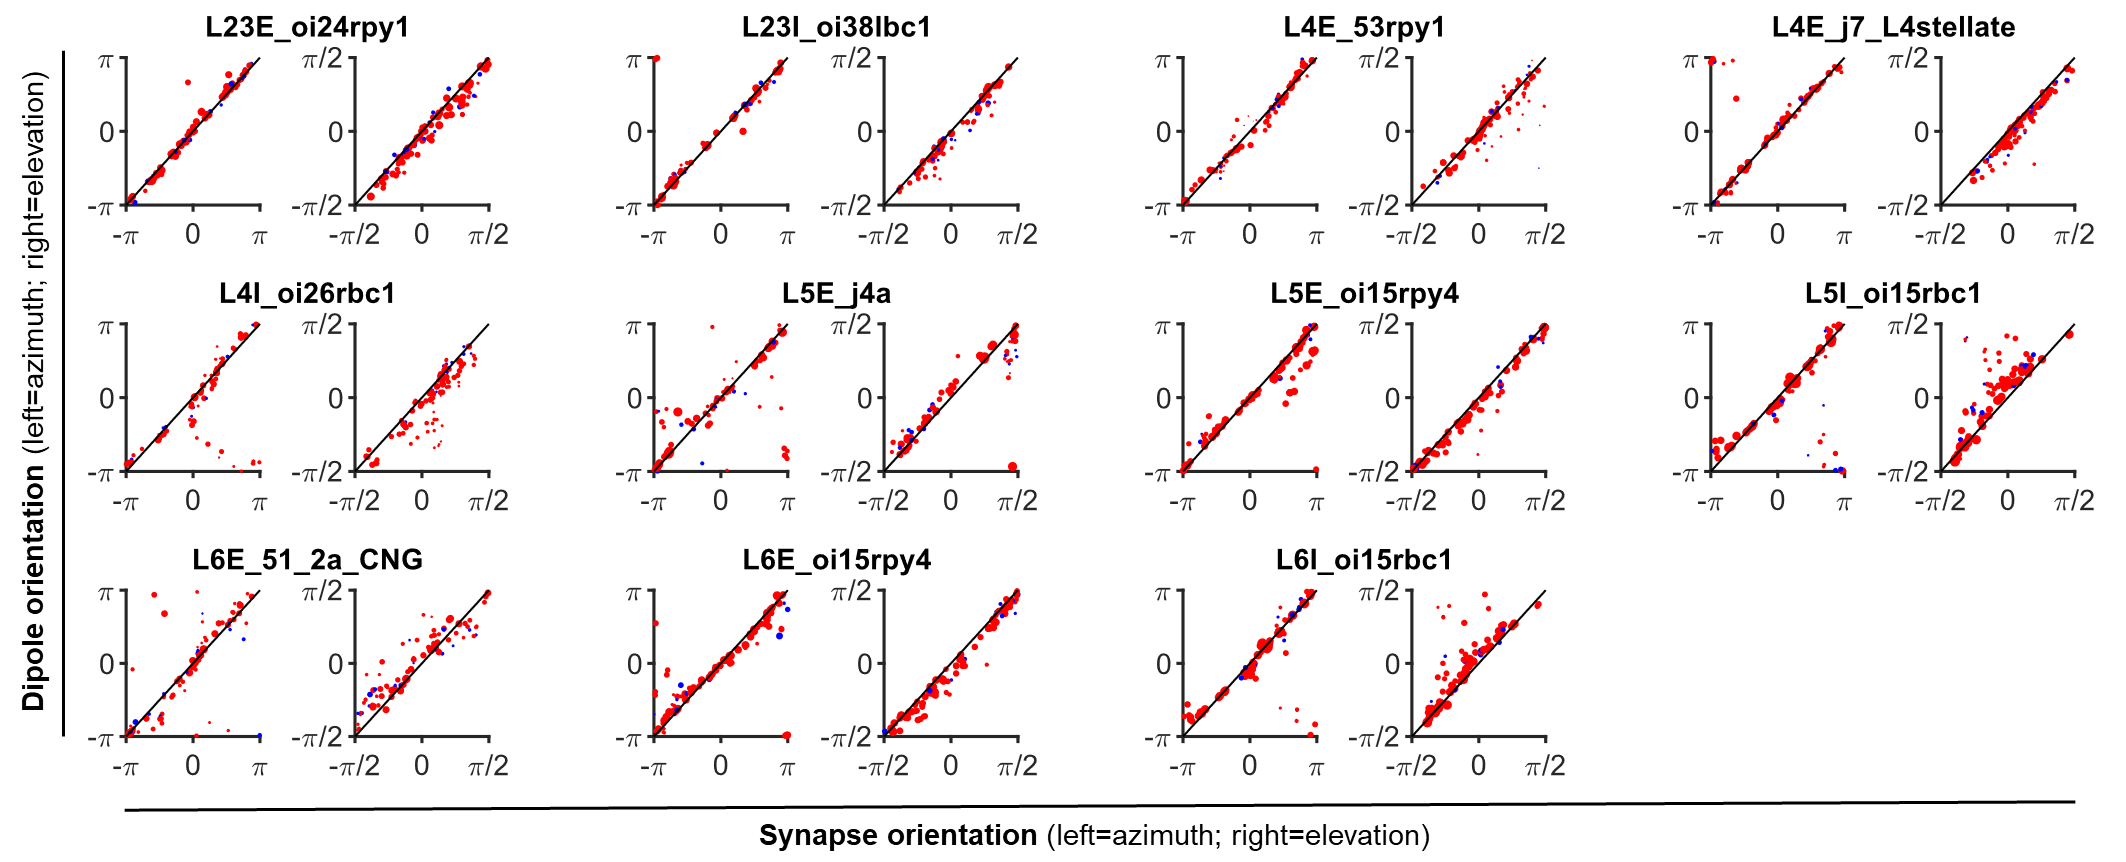
\includegraphics[width=180mm]{Figures/chapter2/figureS1.png}}
\centerline{
\begin{minipage}[c]{180mm}
\captionof{figure}{\captiontitle{Relationships between synapse orientation and dipole orientation.}
Dipole moments were simulated following a single synapse activation at various locations across the 11 representative neuron morphologies (\autoref{tab:tableS2.1}). For each morphology, two plots are shown: the left plots show the azimuth of the dipole moment plotted against that of the synapse that was activated; the right plots show the elevations. Red dots reflect excitatory synapses and blue dots reflect inhibitory synapses. Unity lines are drawn in black.} 
\label{fig:figureS2.1}
\end{minipage}
}
\newpage




\centerline{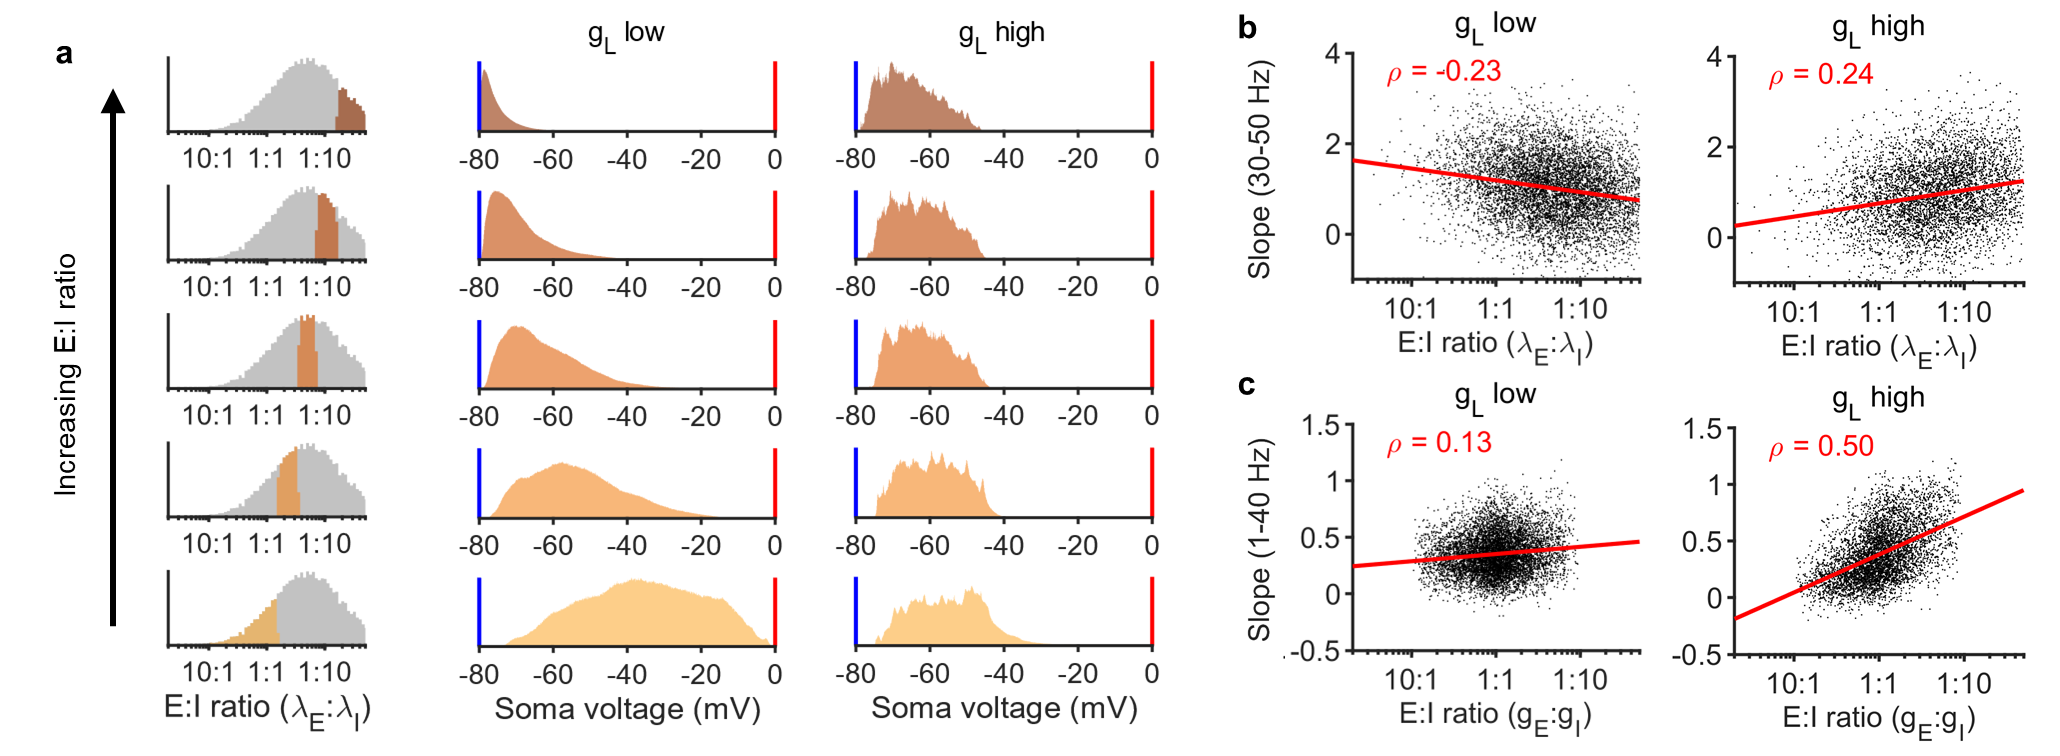
\includegraphics[width=170mm]{Figures/chapter2/figureS2.png}}
\centerline{
\begin{minipage}[c]{170mm}
\captionof{figure}{\captiontitle{Effects of excitatory-inhibitory ratio on membrane potential and spectral slope depend on leak conductance.}
\textbf{a} Left: histogram of E:I ratios across 20,000 simulations with parameters sampled from the distributions in Fig. 6a. Simulations were binned into five categories, from low to high $\lambda_E$:$\lambda_I$ ratios. Middle: histogram of somatic membrane potential for simulations with a low leak conductance ($g_L < 1$ \unit{\milli\siemens\per\centi\meter\squared}), divided into the five E:I ratio categories. The average membrane potential is not largely affected by the E:I ratio in this high leak conductance condition. Right: histogram of somatic membrane potential for simulations with a high leak conductance ($g_L > 1$ \unit{\milli\siemens\per\centi\meter\squared}). A high E:I ratio significantly shifts the distribution of membrane potential to more hyperpolarized values. Blue and red vertical lines show the reversal potential of GABARs and AMARs, respectively.
\textbf{b} Same as Fig. \ref{fig:figure2.6}e, but for the slope computed between 30-50 Hz for $g_L$ high ($\rho=0.24$; $R^2=0.06$; $p<10^{-6}$; $n=5184$ simulations) and $g_L$ low ($\rho=-0.23;$ $R^2=0.05$; $p<10^{-6}$; $n=7366$ simulations).
\textbf{c} Same as \ref{fig:figure2.6}e, but with the E:I ratio defined as the ratio between $g_E$ and $g_I$ , for $g_L$  high ($\rho=0.50$; $R^2=0.25$; $p<10^{-6}$; $n=5184$ simulations) and $g_L$ low ($\rho=0.13$; $R^2=0.02$; $p<10^{-6}$; $n=7366$ simulations).} 
\label{fig:figureS2.2}
\end{minipage}
}
\newpage


\centerline{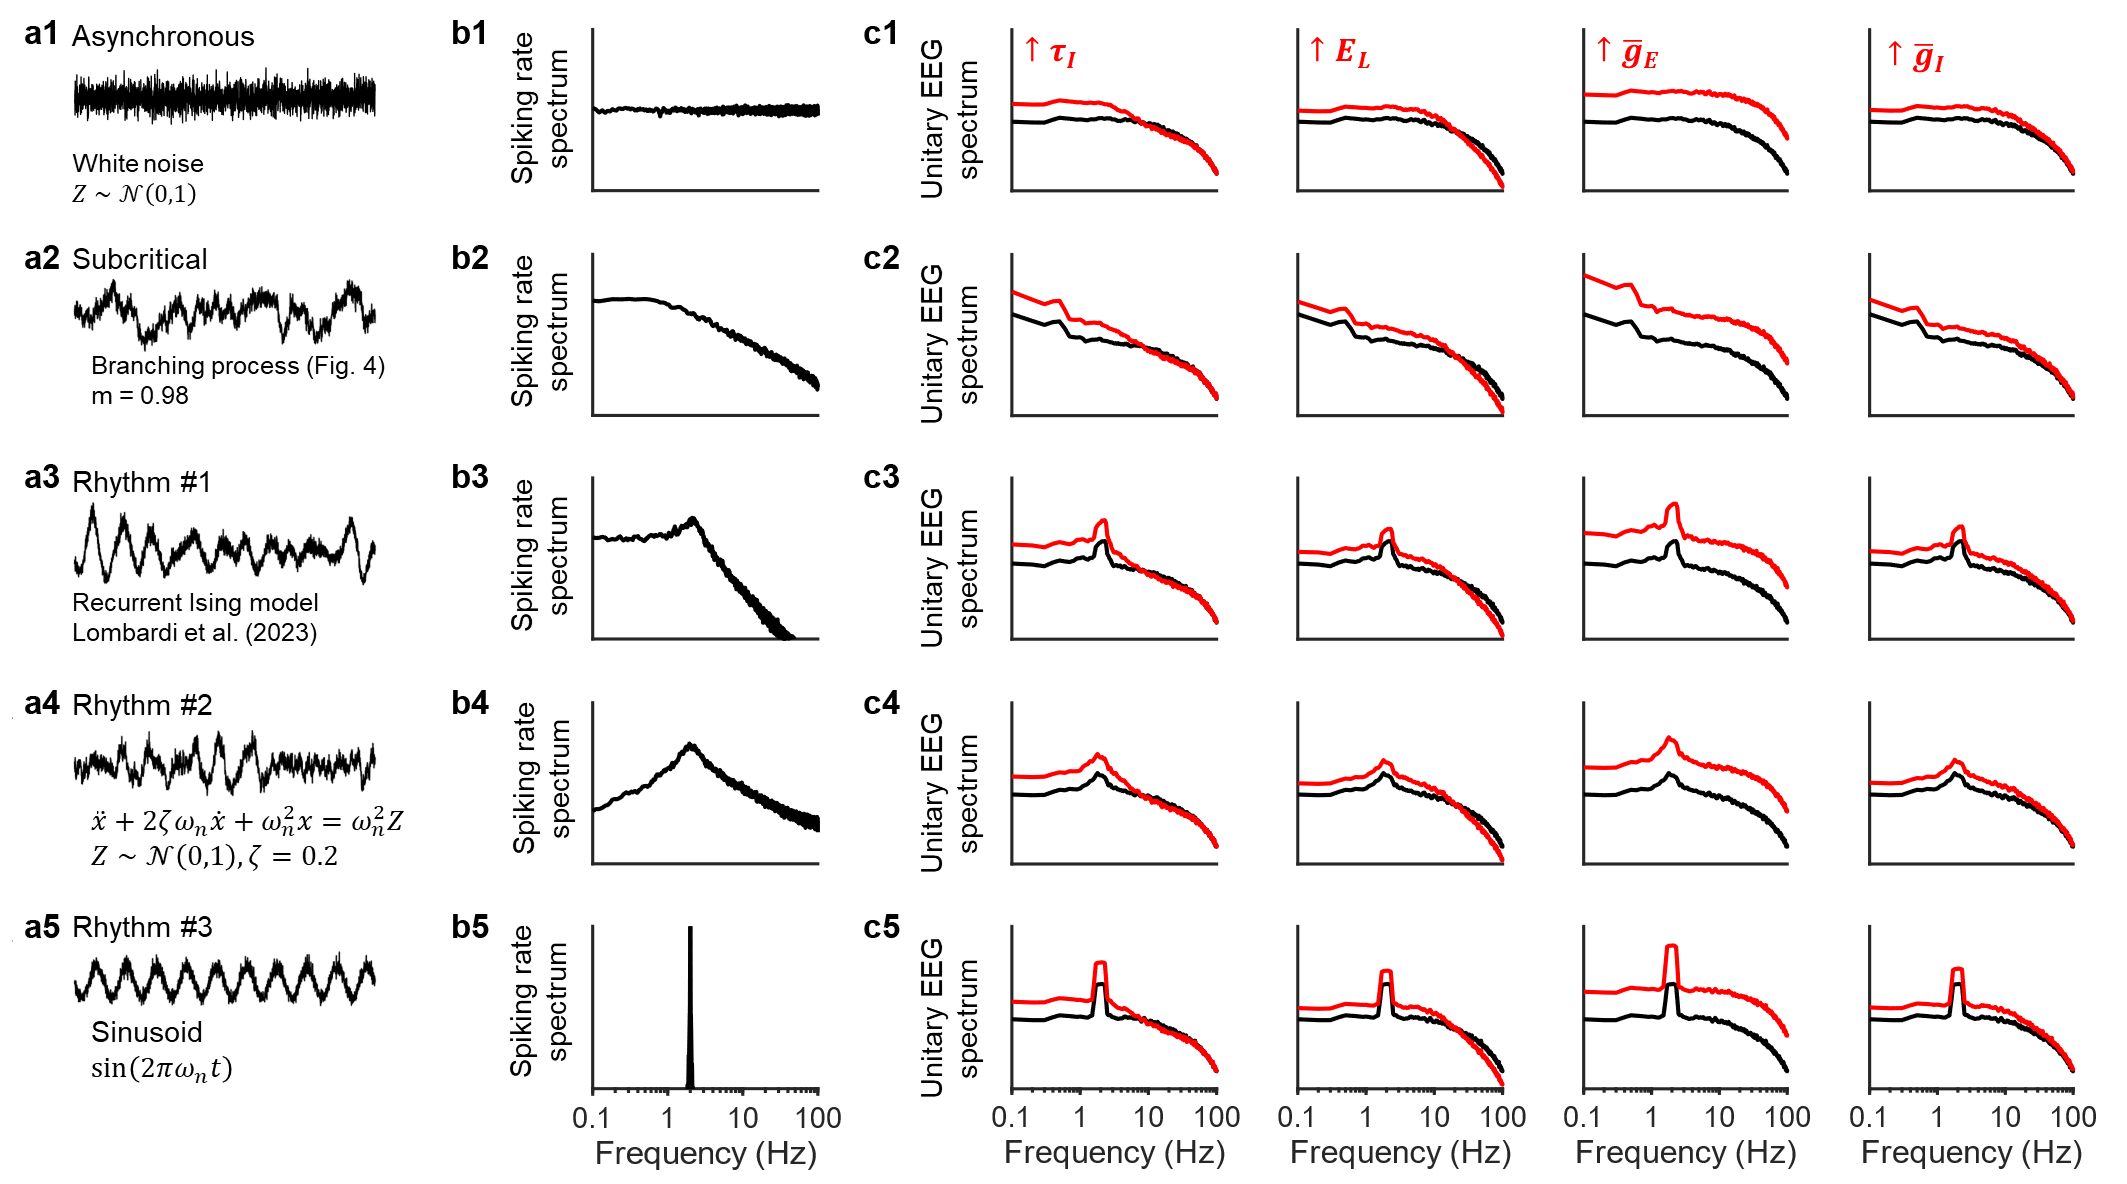
\includegraphics[width=180mm]{Figures/chapter2/figureS3.png}}
\centerline{
\begin{minipage}[c]{180mm}
\captionof{figure}{\captiontitle{Biophysical parameters alter broadband EEG properties across many types of dynamics.}
\textbf{a1}-\textbf{a5}	Five examples of synaptic input dynamics, generated by asynchronous white noise (\textbf{1}), a subcritical branching process (\textbf{2}), a recurrent Ising model \cite{Lombardi2023} (\textbf{3}), an underdamped second-order linear system (\textbf{4}), and a sine wave (\textbf{5}). $\alpha_x=0.1$ for all simulations in this figure.
\textbf{b1}-\textbf{b5}	Power spectra of the rate functions for each type of synaptic input depicted in (\textbf{a1}-\textbf{a5}), respectively. 
\textbf{c1}-\textbf{c5}	Unitary spectra associated with input depicted in \textbf{a1}-\textbf{5}, before and after changes to a biophysical parameter, including $\tau_I$ that was increased from \qty{10}{\milli\second} (black) to 30~\unit{\milli\second} (red) in the first column, $E_L$ that was increased from \qty{-60}{\milli\volt} (black) to \qty{-45}{\milli\volt} (red) in the second column, and $g_E$ and $g_I$ that were increased from \qty{0.7}{\nano\siemens} (black) to \qty{1.4}{\nano\siemens} (red) in the third and fourth columns, respectively.
.} 
\label{fig:figureS2.3}
\end{minipage}
}
\newpage


\centerline{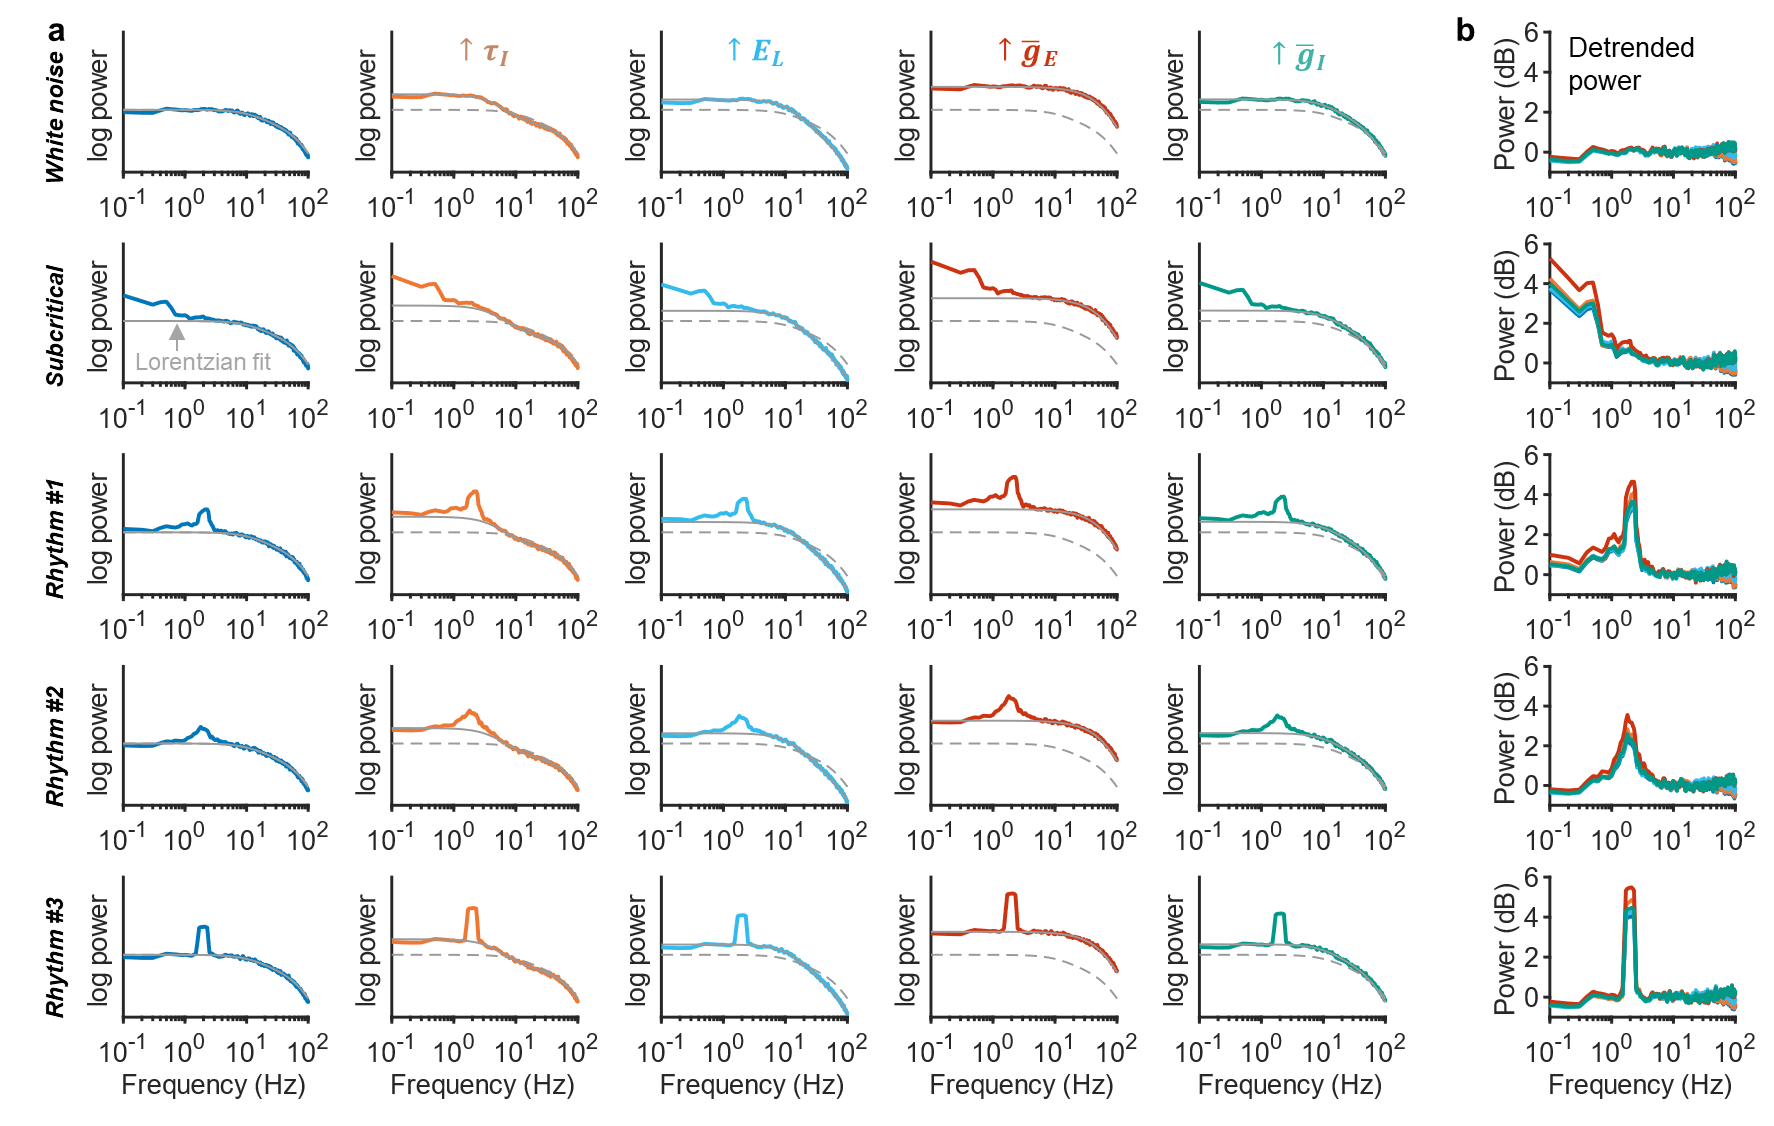
\includegraphics[width=150mm]{Figures/chapter2/figureS4.png}}
\centerline{
\begin{minipage}[c]{\textwidth}
\captionof{figure}{\captiontitle{Detrending with Lorentzian function corrects for changes in biophysical parameters.}
\textbf{a}	Unitary spectra from Fig. \ref{fig:figureS2.3}, fit with the sum of two Lorentzian functions (Eq. 1; solid gray lines). The leftmost column shows the unitary spectrum with default parameters. The Lorentzian fit for the default parameters are also displayed in the plots in the other columns as a dashed grey line.
\textbf{b}	Unitary spectra from (\textbf{a}), detrended by dividing by the fitted Lorentzian function (solid gray lines). Colours correspond to the various parameter changes from (\textbf{a}). Note that, for each type of input dynamics, the detrended spectra have similar profiles, i.e., the effects of the parameter changes have been corrected.} 
\label{fig:figureS2.4}
\end{minipage}
}
\newpage


\centerline{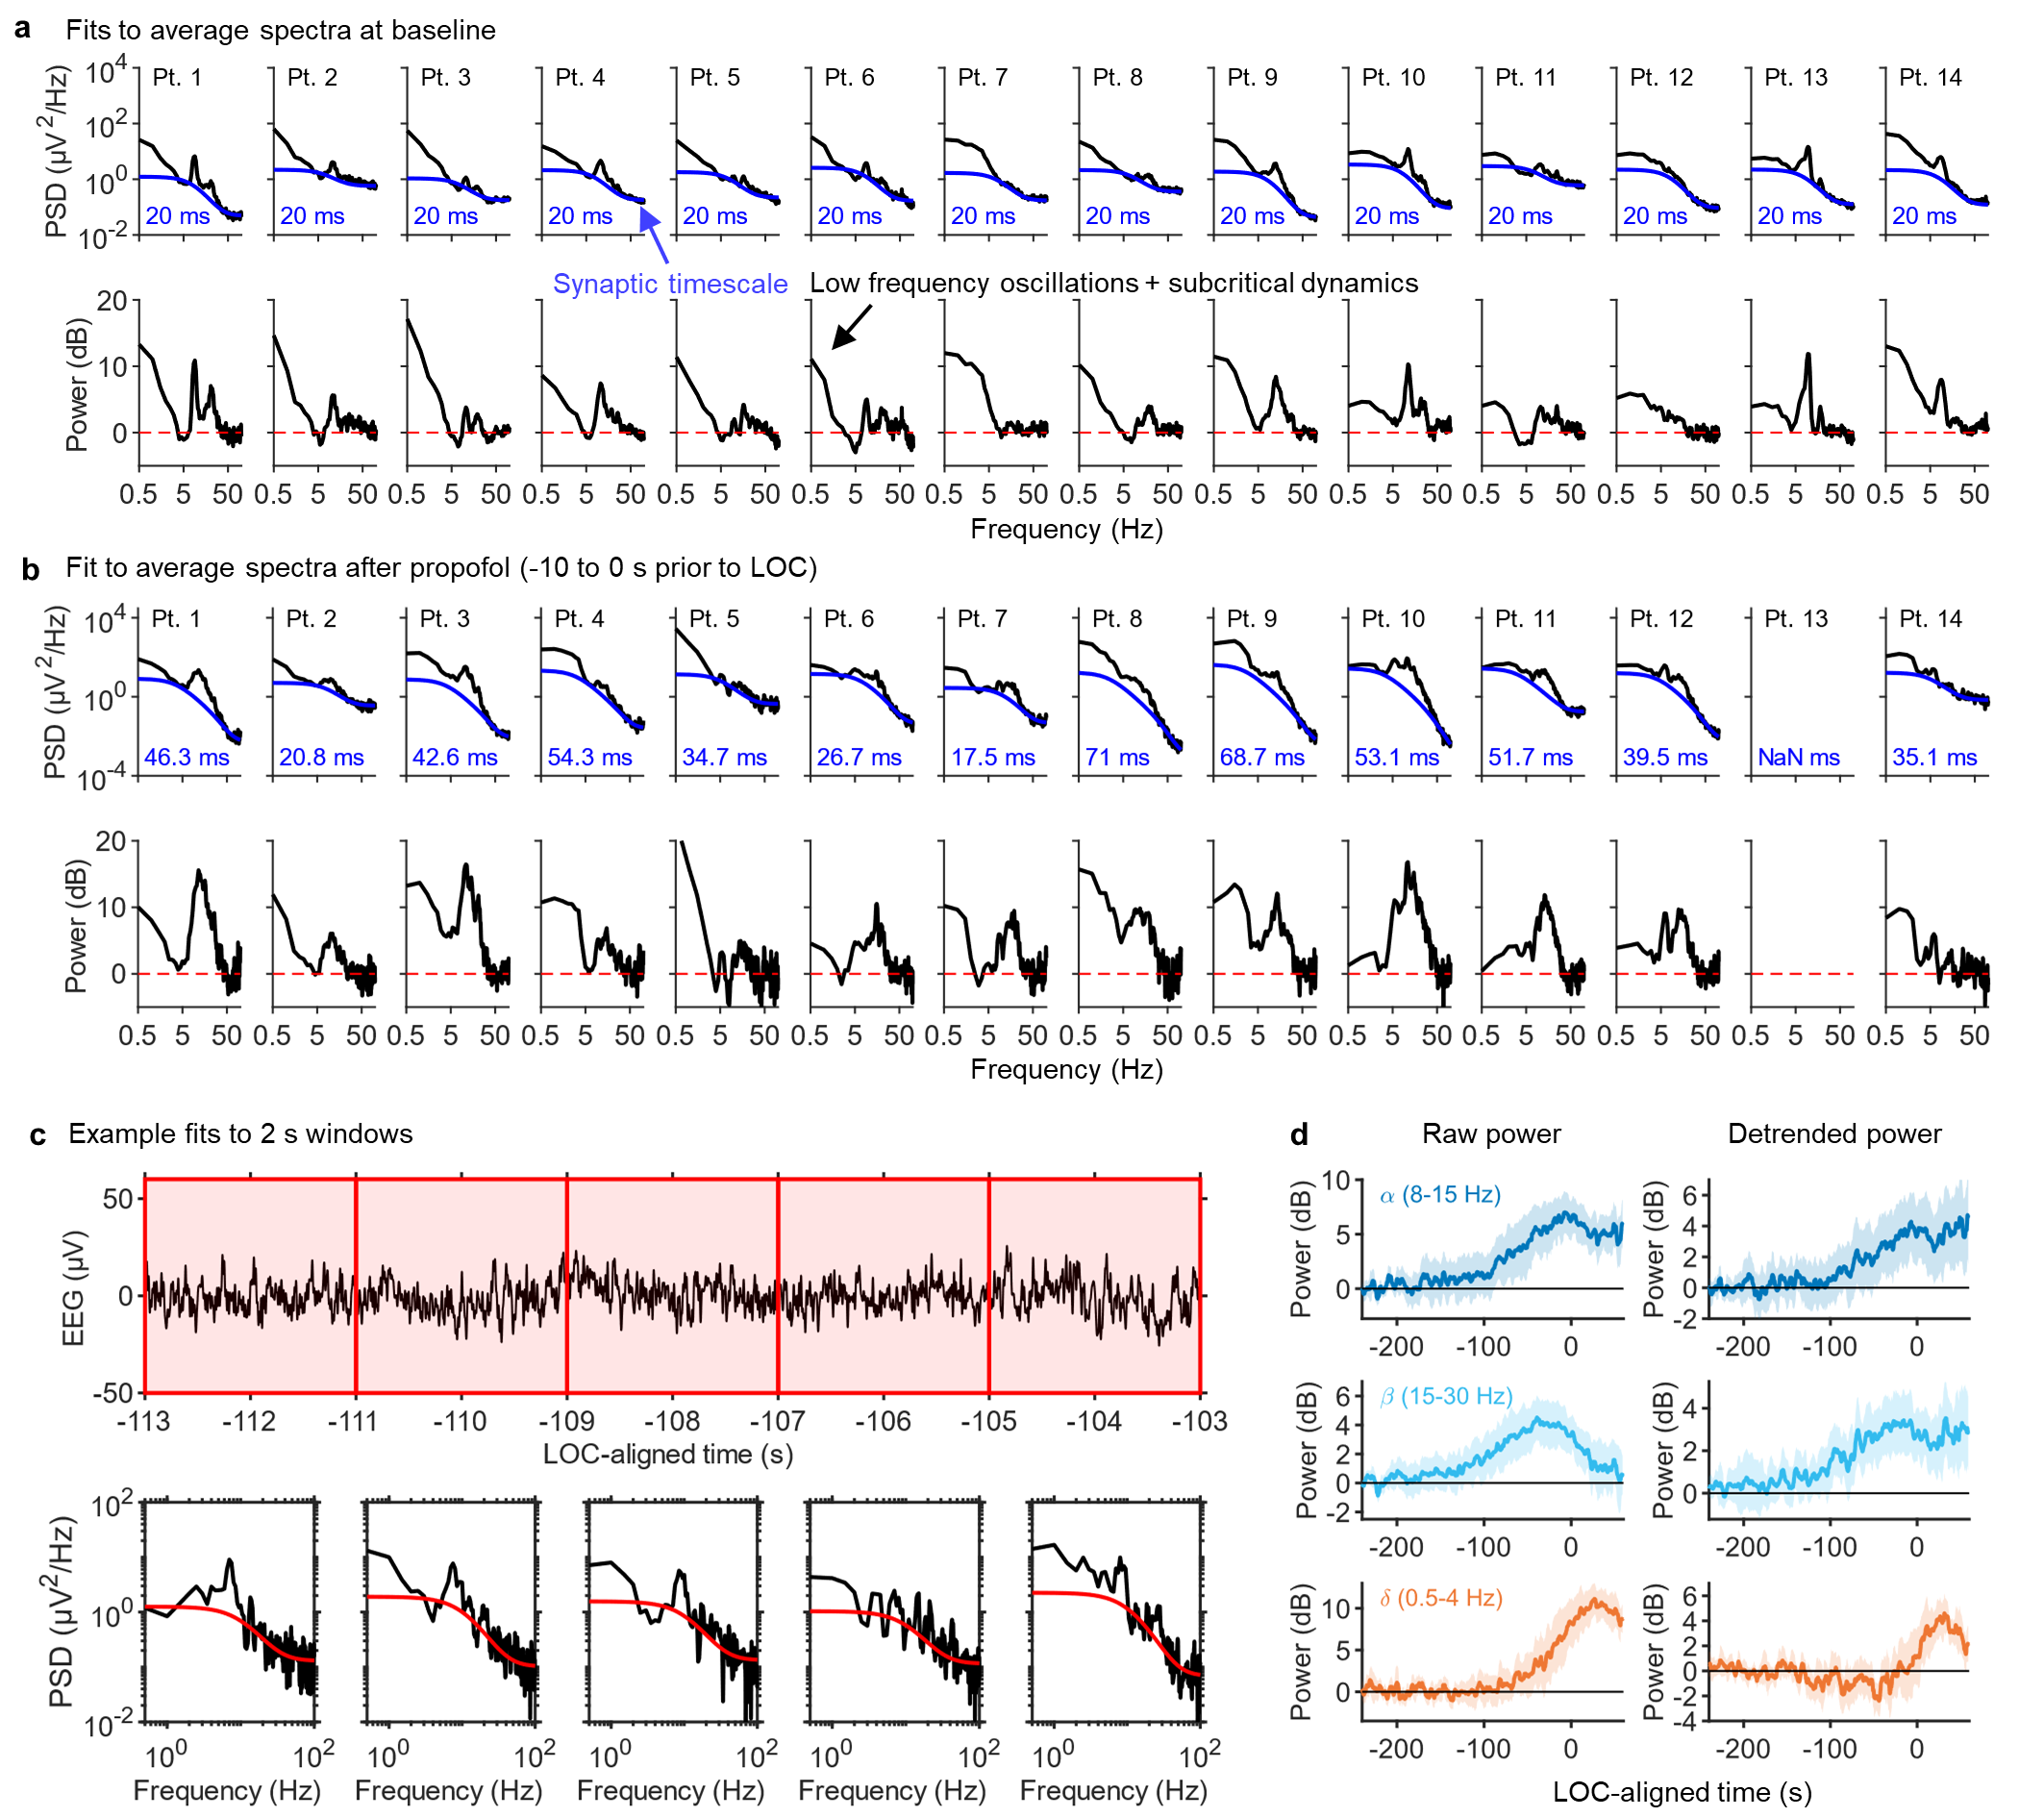
\includegraphics[width=180mm]{Figures/chapter2/figureS5.png}}
\centerline{
\begin{minipage}[c]{180mm}
\captionof{figure}{\captiontitle{Spectral changes with respect to LOC-aligned time.}
\textbf{a} Top: example fits to the average EEG spectrum of each patient at baseline using Eq. \ref{eq:fitting}, while fixing the parameters $\tau_r=4$ \unit{\milli\second} and $\tau_1=20$ \unit{\milli\second}. Note the difference between the fitted Eq. \ref{eq:fitting} and the low frequency power ($< 3$ \unit{\hertz}), which our model predicts is caused by neural dynamics and not synaptic timescales. This low frequency power was fit here with a Gaussian peak function as per the FOOOF methods \cite{Donoghue2020}  fits not shown). Bottom: detrended power in decibels.
\textbf{b} Same as a, but for fits to spectra -10 to 0~\unit{\second} prior to LOC. Here, $\tau_1$   was not fixed and its estimated value for each patient is printed in blue.
\textbf{c} Example EEG from patient 13, split into five, 2 s windows (top). The power spectrum of each window is shown below, along with the fitted synaptic timescales (Eq. \ref{eq:fitting}) in red. 
\textbf{d} Same as Fig. \ref{fig:figure2.9}d \& h, but band power is plotted here against time relative to LOC. Data plotted as mean and shading represents 95\% confidence interval of mean.} 
\label{fig:figureS2.5}
\end{minipage}
}
\newpage

 
\begin{minipage}{\linewidth}
    \centerline{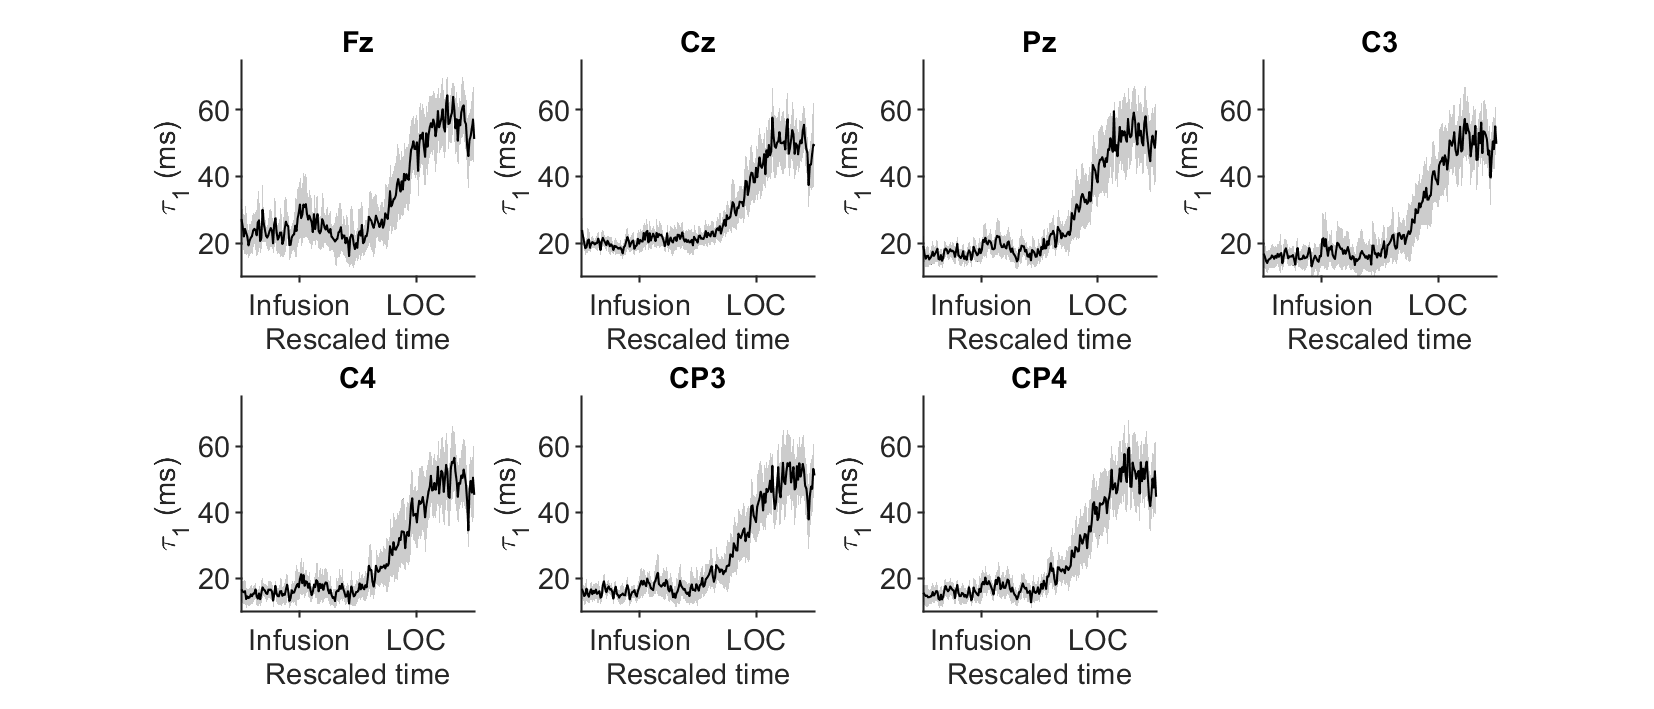
\includegraphics[width=120mm]{Figures/chapter2/figureS6.png}}
    \centerline{
    \begin{minipage}[c]{\textwidth}
    \captionof{figure}{\captiontitle{Changes in estimated $\tau_1$ exhibit similar dynamics across recording locations.}
    The plot labelled Cz is identical to Fig. \ref{fig:figure2.8}e. The other plots show the dynamics of $\tau_1$ for the other EEG channels. For each plot, the corresponding recording site is printed above.} 
    \label{fig:figureS2.6}
    \end{minipage}
    }
\end{minipage}
 

 \begin{minipage}{\linewidth}
    \centerline{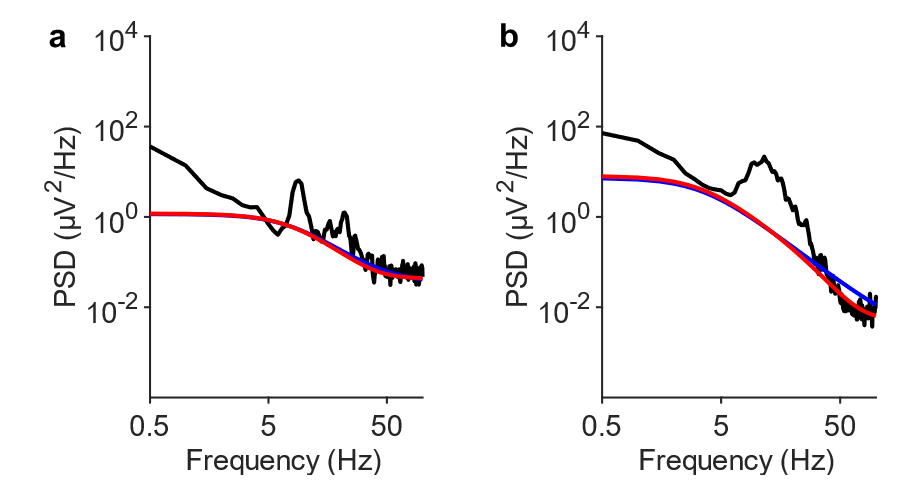
\includegraphics[width=77mm]{Figures/chapter2/figureS7.png}}
    \centerline{
    \begin{minipage}[c]{\textwidth}
    \captionof{figure}{\captiontitle{Simple exponential decaying synaptic response does not capture spectral trend following propofol infusion.}
    \textbf{a} Example spectrum of subject 1 at baseline, same as in Fig. \ref{fig:figure2.8}d. Blue line: data fitted with Eq. \ref{eq:fitting_no_tau2}; $\tau_1=20$ \unit{\milli\second}, $A_1=56$, and $\lambda=0.034$. Red line: data fitted with Eq. \ref{eq:fitting}; $\tau_1=20$ \unit{\milli\second}, $\tau_2=4$ \unit{\milli\second}, $A_1=4470$, and $\lambda=0.043$.
    \textbf{b} Example spectrum of subject 1 following propofol infusion, 0 to 10 s prior to LOC, same as in Fig. \ref{fig:figure2.8}d. Blue line: data fitted with Eq. \ref{eq:fitting_no_tau2}; $\tau_1=46$ \unit{\milli\second}, $A_1=158$, and $\lambda=0.0026$. Red line: data fitted with Eq. \ref{eq:fitting}; $\tau_1=46$ \unit{\milli\second}, $\tau_2=4$ \unit{\milli\second}, $A_1=4570$, and $\lambda=0.0051$. Note that the blue line is not steep enough to capture the drop-off in power around \qty{30}{\hertz}.
} 
    \label{fig:figureS2.7}
    \end{minipage}
    }
\end{minipage}

\newpage

\subsection{Supplementary tables}

\begin{minipage}{\linewidth}
    \captionof{table}{\captiontitle{Representative neuron morphologies used in the model\textsuperscript{a}.}}
    \label{tab:tableS2.1}
    \vskip-\abovecaptionskip
    \vskip+\belowcaptionskip
    \small
    % \centering
    \begin{tabular}{lrlll}
        \hline
        \textbf{Cell type} & \textbf{Abundance (\%)}  & \textbf{Internal ID} & \textbf{External IDs}\textsuperscript{b} & \textbf{References} \\
        \hline
        Layer 2/3 pyramidal cell            &  26.8 &  L23E\_oi24py1      &  NMO\_10045   & Ref. \citen{Budd2010}  \\
        Layer 2/3 interneuron               &   7.5 &  L23I\_oi38lbc1     &  -           & Ref. \citen{Stepanyants2008} \\
        Layer 4 excitatory stellate cell    &  19.0 &  L4E\_j7\_L4stellate &  NMO\_00905   & Ref. \citen{Mainen1996} \\
        Layer 4 pyramidal cell              &   9.5 &  L4E\_53rpy1        &  NMO\_10040   & Ref. \citen{Budd2010} \\
        Layer 4 interneuron                 &   7.1 &  L4I\_oi26rbc1      &  -           & Ref. \citen{Stepanyants2008} \\
        Layer 5 pyramidal cell              &   4.9 &  L5E\_oi15rpy4      &  NMO\_10046   & Ref. \citen{Budd2010} \\
        Layer 5 interneuron                 &   1.4 &  L5I\_oi15rbc1      &  -           & Ref. \citen{Stepanyants2008} \\
        Layer 5 tufted pyramidal cell       &   1.3 &  L5E\_j4a           &  MDB\_2488    & Ref. \citen{Mainen1996} \\
        Layer 6 excitatory cell             &  14.0 &  L6E\_51\_2a\_CNG     &  NMO\_00879   & Ref. \citen{Contreras1997} \\
        Layer 6 pyramidal cell              &   4.6 &  L6E\_oi15rpy4      &  -           & Ref. \citen{Budd2010} \\
        Layer 6 interneuron                 &   3.8 &  L6I\_oi15rbc1      &  -           & Ref. \citen{Stepanyants2008} \\
        \hline
    \end{tabular}
    \vskip-\abovecaptionskip
    \vskip+\belowcaptionskip
    \singlespacing
    \footnotesize
    \begin{flushleft}
        \textsuperscript{a}Morphologies and relative abundances were identical to Hagen et al.\cite{Hagen2018} \\
        \textsuperscript{b}Morphologies without NeuorMoprho (NMO) or ModelDB (MDB) IDs were accessed from the code repository associated with Hagen et al.\cite{Hagen2018} All morphology files are also supplied in the code repository associated with this paper\cite{niklas_brake_2023_10359818}.
    \end{flushleft}
\end{minipage}

\vspace{1em}

\noindent
\setlength{\tabcolsep}{2pt}
\begin{minipage}{\linewidth}
    \captionof{table}{\captiontitle{In vitro data on inhibitory synapse kinetics in the presence of propofol.}} \label{tab:tableS2.2}
    \vskip-\abovecaptionskip
    \vskip+\belowcaptionskip
    \small
    \begin{tabular}{l|rrr|rrrrr|rrrrrr|rrrrrr}
        \hline
        & \multicolumn{3}{c|}{Study \#1\textsuperscript{a}} & \multicolumn{5}{c|}{Study \#2\textsuperscript{b}} & \multicolumn{6}{c|}{Study \#3\textsuperscript{c}} & 
        \multicolumn{6}{c}{Study \#4\textsuperscript{d}} \\
        \hline
        Propofol ($\mu$M) & 0 & 0.5 & 2 & 0.1 & 0.3 & 1 & 3 & 10 & 0 & 0.5 & 1 & 2 & 5 & 10 & 0 & 0.5 & 1 & 2 & 5 & 10 \\
        $\tau$ (\unit{\milli\second}) & 19.4 & 29.6 & 44.5 & - & - & - & - & - & 17.5 & 17.5 & 19 & 48 & 58 & 75 & 17.5 & 17.5 & 19 & 22.5 & 50 & 75 \\
        $\tau$ (fold change) & 1 & 1.5 & 2.3 & 1 & 1.2 & 1.4 & 1.5 & 2 & 1 & 1 & 1.1 & 2.7 & 3.3 & 4.3 & 1 & 1 & 1.1 & 1.3 & 2.9 & 4.3 \\
        \hline
    \end{tabular}    
    \vskip-\abovecaptionskip
    \vskip+\belowcaptionskip
    \singlespacing
    \footnotesize
    \begin{flushleft}
        \textsuperscript{a} Inhibitory post-synaptic current (IPSC) decay time constant taken from Fig. 8 of Orser et al. \cite{Orser1994}. \\
        \textsuperscript{b} Fold change in spontaneous IPSCs estimated from Fig. 7C of Kitamura et al. \cite{Kitamura2003}. \\
        \textsuperscript{c} Decay time of IPSCs during slow parts of evoked trains, taken from Fig. 5 of Whittington et al. \cite{Whittington1996}. \\
        \textsuperscript{d} Decay time of IPSCs during fast parts of evoked trains, taken from Fig. 5 of Whittington et al. \cite{Whittington1996}. 
    \end{flushleft}
\end{minipage}

\renewcommand{\thefigure}{\thechapter.\arabic{figure}}
\renewcommand{\figurename}{Fig.}
\setcounter{figure}{0}

\renewcommand{\thetable}{\thechapter.\arabic{table}}
\renewcommand{\tablename}{Table}
\setcounter{table}{0}

% \chapter{T cell receptor affinity in acute vs. chronic pathogen control}
\label{sec:AvC}

With the exception of the preface, the work presented in this chapter constitutes our submitted manuscript, under review at the time of writing, titled ``\secbfcolor{Chronic infection control relies on T cells with lower foreign antigen binding strength generated by N-nucleotide diversity}'' by H. Jamaleddine, D. Rogers, G. Perreault, D. Patel, J.N. Mandl, and A. Khadra. Video files referenced throughout the text can be found in the online preprint of our manuscript, available in~\cite{jamaleddine2022chronic}.


\phantomsection
\section*{Preface}
\addcontentsline{toc}{section}{Preface}

Chapter~\ref{sec:Tr1} outlined the work we had done to understand immunoregulation by therapeutically expanded Tr1 cells. We showed that Tr1 efficacy, based on its antigen specificity and avidity within autoimmune tissues/draining lymph nodes, could largely explain pMHC-NP therapy outcomes from a variety of experimental treatment protocols. Upon completion of this study, we became interested in delving deeper into the role that antigen specificity, and in particular pMHC binding strength, plays in shaping immune responses, this time in the context of infectious pathogen control. More specifically, we wanted to adapt our model presented in Chapter~\ref{sec:Tr1} to try to answer a new set of questions: how do pMHC binding strength distributions, defined along a continuum between the bounds set by positive and negative selection, evolve over the course of an infection, and how might this differ depending on infection duration? Furthermore, can TCR repertoire diversification through non-templated nucleotide additions by TdT (as described in Chapter~\ref{sec:intro_overview_TCRdiversification}) alter the distribution of TCR binding strengths to pMHC, and if so, how might this affect T cell-mediated control of an acute vs. a chronic replicating pathogen? In this chapter, I will outline the modelling work we have done, in collaboration with experimental support generated by the Mandl laboratory, to address these very questions.

\newpage
\section{Abstract}

The breadth of pathogens to which T cells can respond is determined by the T cell receptors (TCRs) present in an individual’s repertoire. Although more than 90\% of the sequence diversity among TCRs is generated by terminal deoxynucleotidyl transferase (TdT)-mediated N-nucleotide addition during V(D)J recombination, the benefit of TdT-altered TCRs remains unclear. Here, we computationally and experimentally investigated whether TCRs with higher N-nucleotide diversity via TdT make distinct contributions to acute or chronic pathogen control. When T cells with high pMHC reactivity have a greater propensity to become functionally exhausted than those of low pMHC reactivity, our computational model predicts a shift toward T cells with low pMHC reactivity over time during chronic, but not acute, infections. This TCR-affinity shift is critical, as the elimination of T cells with lower pMHC-reactivity \textit{in silico} substantially increased the time to clear a chronic infection. Corroborating an affinity-centric benefit for TCR diversity, in experiments using TdT-deficient mice we showed that infection with a chronic viral pathogen led to increased viral loads later in infection, while acute viral control was unaffected. Taken together, our model and experimental data suggest that TdT-mediated TCR diversity is of particular benefit in the control of prolonged pathogen replication.


\section{Introduction}

The generation of lymphocyte receptor diversity is a key feature of adaptive immunity~\cite{cooper2006evolution,schatz2011recombination}. For T cells, this diversity is established by somatic recombination of the V(D)J gene segments that constitute the \textalpha- and \textbeta-chains of the T cell receptor (TCR)~\cite{schatz2011recombination}. The T cell response to any one pathogen consists of a number of T cell clonotypes, each expanded from a rare antigen-specific T cell defined by the unique TCR they express. Every T cell clonotype in a given anti-pathogen response recognizes the same or different antigens in the form of peptides presented by major histocompatibility complexes (pMHC)~\cite{yassai2009clonotype} and T cell clonotypes can differ in their ligand binding strengths by several orders of magnitude~\cite{andargachew2018cd4,kolawole2020relationship}. Recent evidence suggests that heterogeneity among responding T cells in their TCR binding affinity to pMHC, henceforth referred to as pMHC reactivity, correlates with important differences in effector function. For instance, pMHC binding strength in CD4\pos{} T cells has been shown to impact early effector lineage differentiation~\cite{snook2018tcr,ditoro2018differential,van2016tcr}, while among CD8\pos{} T cells it correlates with both their ability to induce target cell lysis and proliferative capacity, and also impacts memory T cell development~\cite{kolawole2020relationship}. However, to what extent the pMHC-reactivity distribution of the T cells that constitute a given response affects how quickly a pathogen can be cleared remains incompletely understood.

Experimental techniques are currently limited in their ability to comprehensively study the temporal evolution of T cell clonotype frequencies with distinct pMHC reactivities that make up the antigen-specific response. One common method of identifying antigen-specific T cells is by pMHC-tetramers, which primarily tag clonotypes on the higher end of the pMHC-reactivity spectrum, while missing most low affinity T cells~\cite{andargachew2018cd4}. Employing pMHC-tetramers also requires \textit{a priori} knowledge of the epitope recognized by the T cell population being investigated – tracking only the T cells that are specific to one epitope rather than the entire population of responding T cells. Two-dimensional (2D) binding assays measuring TCR-ligand binding affinity similarly rely on knowing the specific epitope recognized by the T cells under study~\cite{huang2010kinetics}. Tracking T cell responses by focusing on only a subset of epitope-specific T cells can therefore introduce biases and disregards the contribution of the remaining pathogen-specific T cell population. Complementing experimental results with a theoretical framework that accounts for pMHC reactivity in a T cell repertoire is thus a useful approach to obtaining a clearer understanding of the mechanisms impacting pMHC-reactivity profiles and, consequently, T cell responses to infection.

A critical contribution to the diversification of the T cell repertoire in all jawed vertebrates is made by a DNA polymerase, called terminal deoxynucleotidyl transferase (TdT), that adds non-templated nucleotides to the V(D)J junctions in \textalpha\textbeta{TCRs}~\cite{schatz2011recombination,gilfillan1995mice,cabaniols2001most,litman2010origins}, enhancing TCR repertoire diversity $\sim$10 fold from the germline recombinatorial diversity alone~\cite{davis1988t,murugan2012statistical,zarnitsyna2013estimating}. However, the benefit of the N-diversification mediated by TdT has remained elusive given that TdT-knockout (KO) mice have shown no increased susceptibility to infection, nor any detectable impairment in their response to challenge with an acute pathogen~\cite{gilfillan1995efficient,gilfillan1995mice}. Interestingly, the genetic sequence and structure of TdT is highly conserved across vertebrates~\cite{lee1994isolation,hansen1997characterization}, suggesting a hitherto unclear evolutionary benefit for its mechanism of action. One hypothesis proposed is that TdT introduces TCRs that, on average, possess lower reactivity to foreign pMHC~\cite{vrisekoop2014revisiting}. Indeed, TdT KO T cells are more efficiently positively selected in the thymus~\cite{gilfillan1994more}, suggesting they may have inherently greater pMHC affinity. Moreover, upon influenza A virus infection, the HA\textsubscript{518} epitope-specific CD8\pos{} splenic T cells from TdT KO mice were about 10 times more sensitive to antigenic stimulation as measured by IFN\textgamma{} production than epitope-specific CD8\pos{} T cells from wild type mice, again consistent with the idea that TdT-independent TCRs have higher ligand affinity~\cite{haeryfar2008terminal}. Importantly, during chronic antigen stimulation in infection and cancer mouse models alike, T cells with higher pMHC-reactivity have been shown to be more prone to exhaustion, whereby their cytokine production and contribution to pathogen or tumour control is substantially impaired over their low-affinity counterparts~\cite{wherry2003viral,alexander1996role,shakiba2021tcr}. Thus, TdT-dependent TCRs may confer an advantage during chronic infections if the more germline TCRs with higher pMHC-reactivity are more likely to become exhausted and ineffective.

Here, we sought to generate a theoretical framework to examine the role of heterogeneity in T cell reactivity to foreign pMHC in the clearance of an acute or chronic pathogen. To predict the impact of a TdT-deficient T cell repertoire on infection outcomes, we developed and implemented a computational model capturing the kinetics of both acute and chronic pathogen replication that also explicitly considered the evolution of TCR affinity distributions during infection. Our simulations showed that, during chronic infection, there was a decrease in the average pMHC reactivity of the antigen-specific T cell population. Importantly, our model suggested that when the TCR repertoire lacked T cells with lower pMHC reactivity, pathogen clearance during chronic, but not acute, infection was delayed. In line with these model predictions, chronic lymphocytic choriomeningitis virus (LCMV) infection of mice with TdT KO T cells led to more protracted viral replication and a significant delay in viral clearance. Taken together, our modeling and experimental results support the notion that one evolutionary benefit of TdT may be to increase the frequency of T cells with lower pMHC reactivity, and in doing so providing better control of ongoing pathogen replication during chronic infection and preventing them from persisting for longer periods of time within the host.


\section{Results}

\subsection{T cell population model captures kinetics of viral load for both acute and chronic infections}

\begin{figure}[htb!]
    \centering
    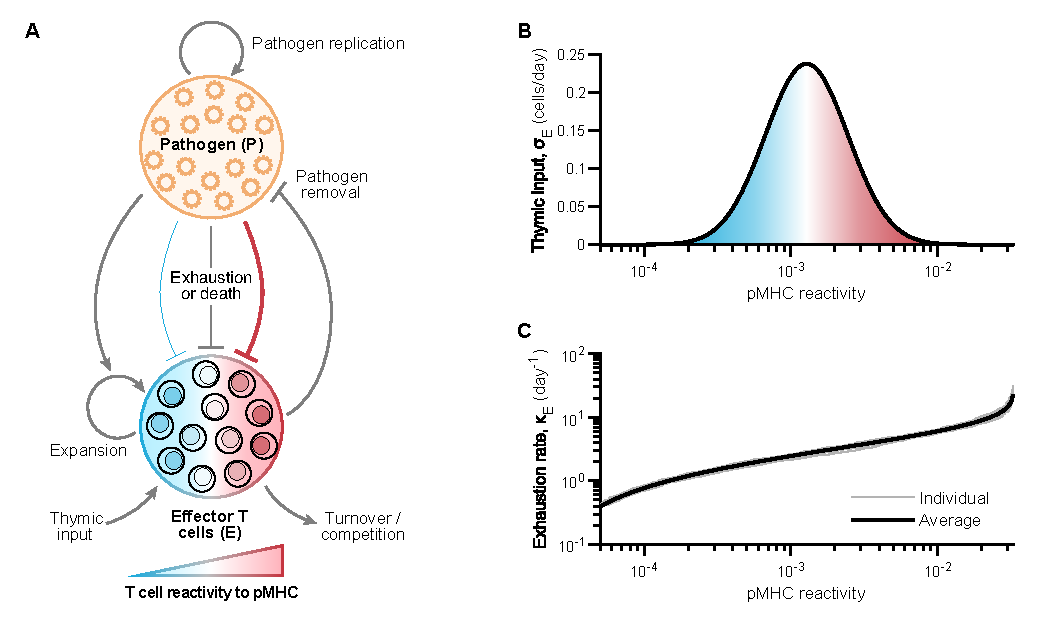
\includegraphics[width=\textwidth]{Figures/AvC/fig1_scheme.pdf}
    \caption[Implementing a computational population model defining the dynamics of pathogen replication and responding T cell clonotypes]{\textit{Implementing a computational population model defining the dynamics of pathogen replication and responding T cell clonotypes}. %
    %
    \secbfcolor{(A)}~Model scheme illustrating model variables and their interactions. The model is described by a system of integro-differential equations that govern the rates of change of the two key players, namely pathogen loads ($P$) and the effector T cells ($E$) that are specific for pathogen-derived antigens in the form of pMHC. The effector T cell population, encompassing the complete collection of pathogen-specific CD4\pos{} and CD8\pos{} T cells, are defined on a continuum according to their overall reactivity to pMHC ($a_k$), i.e., the strength of the overall TCR-pMHC interactions (the shade from blue to red represents the reactivity continuum of T cells to pMHC that ranges from low to high TCR affinities, respectively). Pathogen load is subject to replication as well as negative regulation by effector T cells. Effector T cells expand upon pathogenic exposure, with a constant low-level thymic input, natural turnover, and inter-cellular competition. Pathogen persistence promotes T cell exhaustion and/or activation-induced cell death, with higher pMHC-reactivity T cells more susceptible to these than their low pMHC-reactivity counterparts. For simplicity, we (i)~left out the role of other players such as antigen-presenting cells and B cells from the model in order to focus on the specific role of pMHC reactivity in defining dynamics, and~(ii) did not explicitly distinguish between the action of CD4\pos{} and CD8\pos{} T cells. %
    %
    \secbfcolor{(B,~C)}~Functions depicting pMHC reactivity-dependent parameter values, wherein thymic input~(B), $\sigma_E=f(a_k)$, mimics the shape of a theoretical log-normal distribution, and T cell exhaustion rate~(C), $\kappa_E$, is determined by sampling from a shifted exponential distribution of a set mean, and sorted in ascending order by assigning smaller depletion rates to T cells of low pMHC-reactivity, and vice versa, producing variability between model simulation runs (shown by gray traces obtained from 25 individual model simulations).}
    \label{fig:AvC_scheme}
\end{figure}

In order to compare the temporal evolution of pMHC reactivities of responding T cell clonotypes during acute and chronic infections, we first needed a simple computational model that could recapitulate the kinetics of both rapidly cleared and prolonged pathogen replication. We developed a model that could replicate the serum viral loads obtained upon infection with two strains of LCMV that differ by only 3 coding point mutations, Armstrong (LCMV-Arm) and Clone 13 (LCMV-Cl13), and produce the time course of acute and chronic viral loads in the host, respectively~\cite{wherry2003viral,bergthaler2010viral,ahmed1984selection}. Importantly, the single amino acid mutations between LCMV-Arm and -Cl13 do not occur in peptide segments from which known T cell specific pMHC epitopes are derived~\cite{abdel2019viruses,kotturi2007cd8+} and thus different infection outcomes are governed exclusively by viral replication dynamics within infected cells~\cite{abdel2019viruses,bergthaler2010viral}. Our model considered key interactions between the pathogen load ($P$) and the pMHC-reactivity continuum of all responding effector CD4\pos{} and CD8\pos{} T cells ($E$) (Fig.~\ref{fig:AvC_scheme}A). The dynamics of $P$ and $E$ depend on the rates of pathogen replication, T cell proliferation and expansion upon antigen encounter, thymic input, homeostatic T cell turnover, and pathogen-induced exhaustion and/or cell death (Fig.~\ref{fig:AvC_scheme}A). To incorporate pMHC reactivity explicitly into our model, we defined the thymic input into the effector T cell pool, $\sigma_E$, to be a function of pMHC reactivity (denoted $a_k$, Fig.~\ref{fig:AvC_scheme}B), a parameter proportional to the strength of TCR signaling (refer to Methods) whereby $a_k$ represents how likely it is that a T cell will proliferate upon antigenic stimulation~\cite{standifer2009changes}. Consistent with previous studies, we assumed that the strength of negative regulatory mechanisms (such as T cell exhaustion and activation-induced cell death) is positively correlated with the pMHC reactivity of a given T cell~\cite{wherry2003viral,alexander1996role,shakiba2021tcr}. Variability in model outcomes is generated by randomization of this T cell exhaustion rate, which is selected from a shifted exponential distribution and sorted in increasing order as a function of pMHC reactivity (with a mean determined by model fitting, see Methods) (Fig.~\ref{fig:AvC_scheme}C).

Model parameters (Table~\ref{tab:AvC_parameters}) were obtained by fitting simulated pathogen loads to serum data of LCMV infections from Wherry et al.~\cite{wherry2003viral} using a genetic algorithm (Fig.~\ref{fig:AvC_supp_timeSeries}A,~B). Given that previous work showed LCMV-Cl13 replicates more rapidly in infected cells than LCMV-Arm~\cite{bergthaler2010viral}, we set the replication rate (denoted $r_P$) for our simulated chronic viral infection to be higher than for the acute infection, while keeping all other parameters consistent between the two conditions. By modulating only the pathogen replication rate, we produced time courses that qualitatively matched both LCMV-Arm and LCMV-Cl13 replication dynamics (Fig.~\ref{fig:AvC_timeSeries}A,~B, and Fig.~\ref{fig:AvC_supp_timeSeries}A,~B).
%
\begin{figure}[htb!]
    \centering
    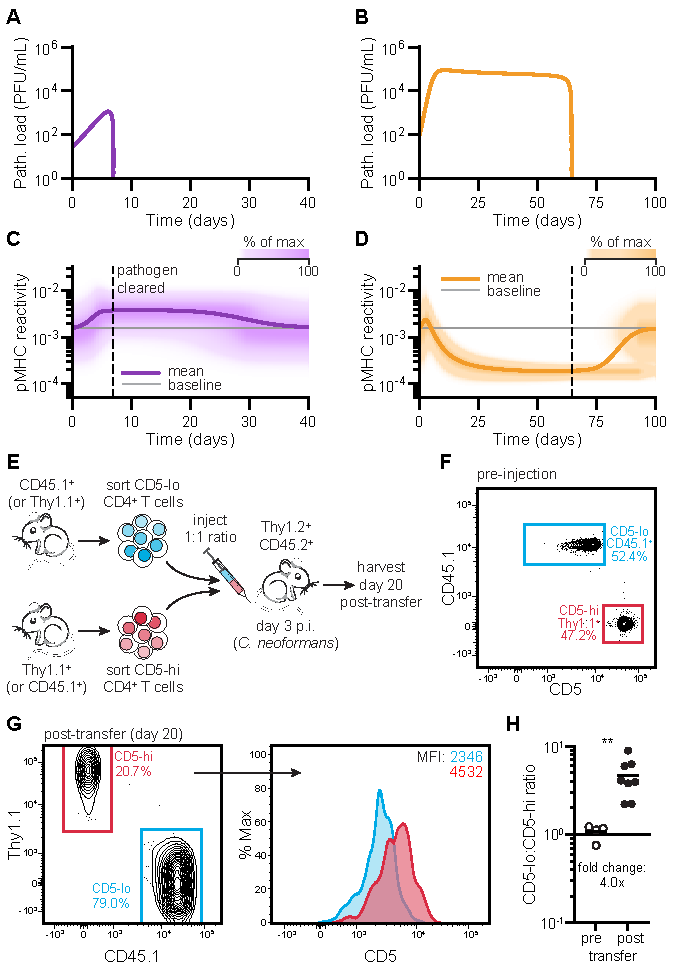
\includegraphics[width=0.64\textwidth]{Figures/AvC/fig2_timeSeries.pdf}
    \caption[T cell pMHC reactivity evolution over time during a T cell response differs between acute and chronic infections]{%
    \textit{T cell pMHC reactivity evolution over time during a T cell response differs between acute and chronic infections}. %
    %
    \secbfcolor{(A-D)} Simulations of pathogen loads and T cell levels in time during acute~(A,~C) or chronic~(B,~D) infection, showing time series simulations of pathogen loads~(A,~B) and heat maps representing the relative proportion of T cells across pMHC reactivities~(C,~D). Overlaid traces represent the mean pMHC-reactivity value in time, with the baseline value denoted in gray. Dotted black lines denote the time at which the pathogen is cleared. %
    %
    \secbfcolor{(E)}~Schematic of experimental approach illustrating adoptive cell transfer of a 1:1 ratio of CD5\supr{lo} and CD5\supr{hi} na\"{i}ve CD4\pos{} T~cells (either Thy1.1\pos{} or CD45.1\pos{}) into congenic CD45.2\pos{} Thy1.2\pos{} recipient mice infected 3 days prior with chronic \textit{C. neoformans}. %
    %
    \secbfcolor{(F,~G)}~Representative flow cytometry plot of CD5\supr{lo} CD45.1\pos{} and CD5\supr{hi} Thy1.1\pos{} transferred T cell populations, pre-injection into recipient infected mice~(F), or 20 days post-transfer with CD5 expression levels shown as a histogram and mean fluorescent intensities (MFI) indicated in blue and red text~(G). %
    %
    \secbfcolor{(H)}~Ratio of transferred CD5\supr{lo} to CD5\supr{hi} T~cells, pre-injection or 20 days post-transfer. **, P = 0.004 computed using a two-tailed Wilcoxon rank sum test, data from 2 independent experiments (n=8 mice).}
    \label{fig:AvC_timeSeries}
\end{figure}
%
In our simulations, the acute viral load peaked at 6.0~days post infection, followed by rapid clearance around 6.9~days post infection based on 100 trial simulations (Fig.~\ref{fig:AvC_timeSeries}A, and Fig.~\ref{fig:AvC_supp_timeSeries}C). In contrast, increasing the viral replication rate to simulate chronic viral replication resulted in prolonged infections with a median time to clearance of 64 days (based on 100 trial simulations) (Fig.~\ref{fig:AvC_timeSeries}B, and Fig.~\ref{fig:AvC_supp_timeSeries}C). Thus, our model was able to reproduce pathogen loads characteristic of both acute and chronic infections by modifying only the rate of pathogen replication while keeping all other model parameters constant.

\subsection{Chronic infection skews responding T cell clonotypes toward lower pMHC reactivities}

Having developed our \textit{in silico} model of acute and chronic pathogen infection, we next asked how the pMHC-reactivity profile of the antigen-specific T cell population evolved over time in each case. When we simulated effector T cell responses to acute infection, we found that the pMHC-reactivity profile of T cells shifted toward a higher pMHC-reactivity mean until peak pathogen replication was reached, followed by a gradual return to baseline after the infection was resolved (Fig.~\ref{fig:AvC_timeSeries}C, and Mov.~\ref{mov:AvC_timeSeries}). Of note, the return of the pMHC-reactivity mean value to the pre-infection baseline was a result of omitting a memory T cell compartment from the model, since our focus was on the effector phase of the T cell response. The shift we observed in the pMHC-reactivity profile during acute infection agrees with previous experimental studies showing that T cells with greater pMHC reactivity expand to large numbers more readily upon antigenic stimulation~\cite{busch1999t,king2012t,rosenthal2012low,mandl2013t}.

Next, we investigated whether the dynamics of pMHC reactivity among responding T cell clonotypes differed during chronic infection. In contrast to acute infection, the pMHC-reactivity distribution peaked during the early phases of chronic infection but was followed by a substantial shift toward lower pMHC reactivities, before returning to baseline after infection clearance (Fig.~\ref{fig:AvC_timeSeries}D). This indicated that, as more T cells of high pMHC reactivity became functionally exhausted due to chronic antigen stimulation from persistent virus (and were thus removed from the active effector T cell pool), T cells of progressively lower reactivities to pMHC gradually predominated among responding T cell clonotypes (Fig.~\ref{fig:AvC_timeSeries}D, and Mov.~\ref{mov:AvC_timeSeries}).

To further investigate whether our model was consistent with experimental data, at least for CD4\pos{} T cells, we used a previously identified surface marker proxy for pMHC reactivity, CD5, whose expression level on CD4\pos{} T cells correlates with pMHC binding strength as measured by tetramer fluorescent intensity and whose expression level is maintained post activation~\cite{mandl2013t,azzam1998cd5,rogers2021pre}. We sorted na\"{i}ve CD4\pos{} T cells on the 20\% CD5\supr{lo} and CD5\supr{hi} cells, as previously described~\cite{mandl2013t,rogers2021pre}, mixed the two sorted populations at a 1:1~ratio (identified by congenic markers, CD45.1 or Thy1.1), and adoptively transferred the mix to CD45.2\pos{} Thy1.2\pos{} recipient mice that were infected 3 days earlier with \textit{Cryptococcus neoformans}, a persistent pulmonary fungal pathogen~\cite{schneider2020migration} (Figs.~\ref{fig:AvC_timeSeries}E,~F, and Fig.~\ref{fig:AvC_supp_timeSeries}D,~E). In contrast to what was previously described during acute infections, where the CD5\supr{hi} CD4\pos{} T cells predominated the response on day 8 post infection~\cite{mandl2013t}, in the later stage of the anti-\textit{Cryptococcus} CD4\pos{} T cell response in the lung, the CD5\supr{lo} CD4\pos{} T cells outnumbered CD5\supr{hi} CD4\pos{} T cells 4-fold (Fig.~\ref{fig:AvC_timeSeries}G,~H).

In summary, our modeling results suggest that the temporal evolution of pMHC reactivities of T cells contributing to the response to an acute compared to a chronic infection is distinct, with T cells of lower pMHC reactivities predominating during the chronic infection phase, whereas T cells of greater pMHC reactivity predominate during an acute infection. Our experimental data from CD4\pos{} T cells corroborated this result and is consistent with evidence from studies of both antigen-specific CD4\pos{} and CD8\pos{} T cells that T cells with lower pMHC reactivity predominate during chronic infection~\cite{gallegos2016control,schober2020reverse,tsitsiklis2020unusual}. 

\subsection{The distribution of pMHC reactivities of responding T cells impacts time to infection clearance}

Having established that the pMHC reactivity of effector T cells changed differentially in acute versus chronic infection, we wanted to determine whether the reverse is true, i.e., whether altering the pMHC-reactivity profile of the antigen-specific T cell population would lead to changes in the duration of pathogen replication upon infection using our simulations. To accomplish this, we targeted model parameters affecting either the mode or the span of the T cell pMHC-reactivity distribution to investigate how perturbing these two parameters impact the T cell response to a pathogen. In these simulations, we maintained the pathogen replication rate at a constant value obtained from fitting the model to LCMV-Cl13 viral loads, and used the time at which pathogen burden returned to zero post infection as a measure to assess: (i)~class of infection (i.e., acute vs. chronic), and (ii)~effectiveness of the T cell response in clearing infection. Gradually varying the mode of the pMHC-reactivity profile over 40~logarithmically spaced values between~$10^{-4}$ and~$10^{-2}$ and running 50~independent simulations per mode value revealed three distinct clusters with different durations of infection (Fig.~\ref{fig:AvC_dists}A).
%
\begin{figure}[t]
    \centering
    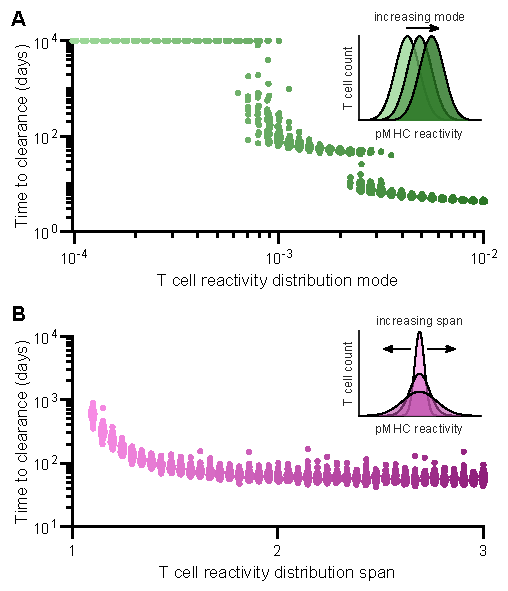
\includegraphics[width=0.48\textwidth]{Figures/AvC/fig3_distributionEffs.pdf}
    \caption[Mode and span of the naïve T cell pMHC-reactivity profile impact pathogen clearance times]{\textit{Mode and span of the naïve T cell pMHC-reactivity profile impact pathogen clearance times}. %
    %
    \secbfcolor{(A, B)}~Time required to clear a replicating pathogen in silico when varying the mode~(A), and the span~(B) of the initial T cell count as a function of pMHC reactivity. Each data point shows the result of a single simulation trial for a given, randomized set of parameters for T cell exhaustion ($\kappa_E$) as determined by the relation defined in Fig.~\ref{fig:AvC_scheme}C. Insets schematically indicate how the T cell count of the starting (pathogen-free/baseline) configuration, as a function of pMHC reactivity, is altered by increasing its mode~(A) or span~(B). The distribution mode and span shown are equivalent to $e^{-(\mu+\sigma^2 )}$ and $e^\sigma$, respectively, where $\mu$ and $\sigma$ are, respectively, the mean and standard deviation of the log-normal pMHC reactivity function defining thymic input (for full details, see Section~\ref{sec:AvC_modelParsFitting}).}
    \label{fig:AvC_dists}
\end{figure}
%
Variability between different runs of the model arise from the randomization of the exhaustion rate, $\kappa_E$, in each simulation, as described previously (Fig.~\ref{fig:AvC_scheme}C). When the mode of antigen-specific pMHC-reactivities of the T cell repertoire was too low (less than $7\E{-4}$), the infection persisted indefinitely, indicating that T cells failed to clear the pathogen. At intermediate values of pMHC reactivity (between $7\E{-4}$ and $2\E{-3}$) the time to clearance was around 100~days, comparable to chronic LCMV-Cl13 infection. When reactivity to foreign pMHC was high, the infection was cleared within 10~days, representative of an acute infection (Fig.~\ref{fig:AvC_dists}A). Varying the span of the pMHC reactivity distribution also affected pathogen replication kinetics, with narrow pMHC reactivity distributions exhibiting impaired chronic pathogen clearance compared to T cell repertoires with broader distributions (Fig.~\ref{fig:AvC_dists}B).

Taken together, our results demonstrate that the pMHC-reactivity profile of responding T cells during infection has a pronounced effect on determining infection duration, with outcomes ranging from rapid pathogen clearance to the complete failure of the T cell response to resolve the infection. Of note, rather than observing gradual shifts in the time to clearance with \textit{in silico} manipulations of the pMHC-reactivity profile, we found sharp jumps between different infection clearance times (namely from acute to chronic, and chronic to indefinitely persistent). By reducing the model to a one-clone, 2-dimensional system of ordinary differential equations and performing bifurcation analysis (Fig.~\ref{fig:AvC_supp_bfns}), we found that distinct solution trajectories through state space are responsible for producing separate clusters of infection durations. Importantly, analysis of the one-clone model showed that, exclusively in the case of chronic pathogen load, the evolution of the T cell profile toward lower pMHC reactivities is responsible for the eventual resolution of chronic infection (Fig.~\ref{fig:AvC_supp_bfns} and Mov.~\ref{mov:AvC_nullclines}, see Section~\ref{sec:AvC_2DmodelAnalysis}).

\subsection{Absence of T cells with low pMHC-reactivity generated by N-nucleotide diversity delays the clearance of chronic infection.}

Our results thus far showed that an increased contribution from T cell clonotypes with low pMHC reactivity could be important in clearing chronic, but not acute, infections. Thus, we next investigated whether populating a TCR repertoire exclusively with higher pMHC reactivity T cells would affect the clearance of either an acute or a chronic infection \textit{in silico}. We tackled this question in two ways. First, in our simulations, we removed T cells with lower pMHC reactivity by eliminating all T cells possessing a pMHC reactivity value below a predefined cut-off threshold without altering the total number of responding T cells, and then progressively increased this threshold to remove up to half of the pMHC reactivity distribution (Fig.~\ref{fig:AvC_modelKO}A). %
%
\begin{figure}[tb]
    \centering
    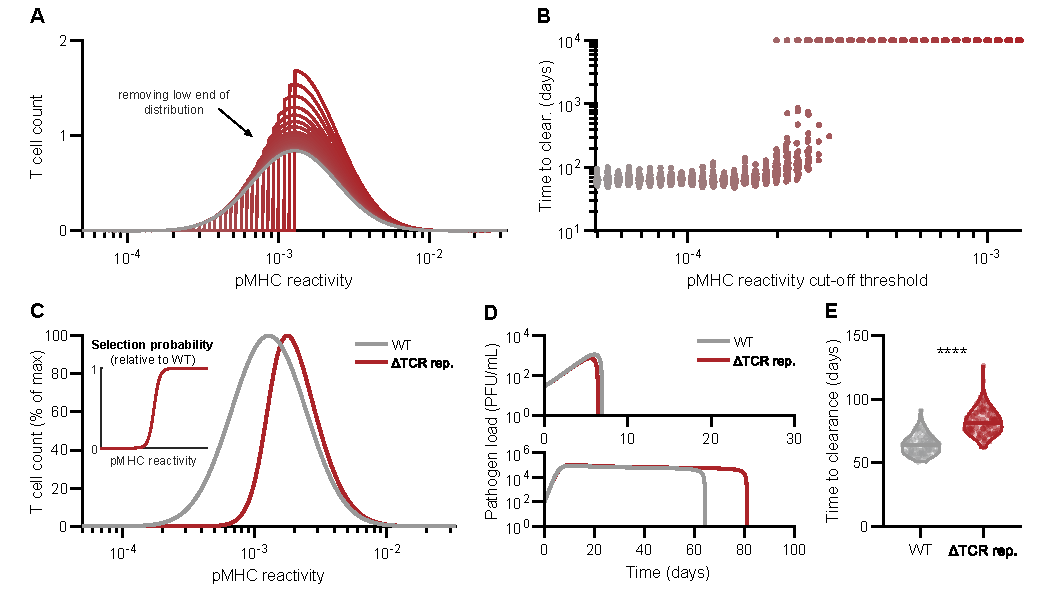
\includegraphics[width=\textwidth]{Figures/AvC/fig4_modelKO.pdf}
    \caption[Deficiency in TCRs with low pMHC-reactivity in silico leads to prolonged chronic, but not acute, pathogen replication]{%
    \textit{Deficiency in TCRs with low pMHC-reactivity in silico leads to prolonged chronic, but not acute, pathogen replication}. % 
    %
    \secbfcolor{(A)}~Distributions of T cells as a function of pMHC reactivity obtained by successively removing low-affinity T cells using different cut-off thresholds from the model’s starting configuration, while keeping the total number of T cells conserved, until only the upper half of the distribution remained. These starting configurations were generated by setting all values of the thymus input, $\sigma_E$, for T cells below a given pMHC-reactivity threshold to 0. \textbf{(B)}~Time to pathogen clearance as a result of increasing the cut-off threshold for T cell reactivity to pMHC corresponding to the configurations shown in A. For each cut-off threshold, 50 simulation trials were performed as described in Fig.~\ref{fig:AvC_dists}. %
    %
    \secbfcolor{(C)}~Theoretical T cell pMHC-reactivity configuration of an altered TCR repertoire (denoted \dTCR{} repertoire) deficient in low-affinity T cells relative to the WT configuration. The \dTCR{} repertoire was assumed to have a lower thymic selection probability (relative to WT repertoire), implying a lower value of the thymic input parameter, $\sigma_E$, for T cells with low pMHC reactivity (see Methods). Inset: Probability of selection, relative to the WT repertoire, for T cells of the \dTCR{} repertoire, with fewer T cells of low reactivity to pMHC being sourced by thymic selection. %
    %
    \secbfcolor{(D)}~Model simulations comparing representative pathogen load traces of WT (gray) or \dTCR{} repertoire (red) systems during acute (top) or chronic (bottom) infection. %
    %
    \secbfcolor{(E)}~Time to clearance of chronic infections for 100 model simulations from WT and \dTCR{} repertoire systems. ****, P = 1.52\E{-25} computed using the Wilcoxon rank sum test.}
    \label{fig:AvC_modelKO}
\end{figure}
%
Our simulations demonstrated that impeding the shift toward lower TCR affinities during a chronic infection by progressively removing T cells with lower pMHC reactivity in this manner dramatically prolonged the time to clearance for the chronic infection cluster, with higher cut-off thresholds leading to failure to clear the chronic pathogen altogether (Fig.~\ref{fig:AvC_modelKO}B). Interestingly, repeating this analysis while decreasing the pathogen replication rate from 1.22~day$^{-1}$ to 1.17 day$^{-1}$ revealed that high cut-off thresholds could result in rapid pathogen clearance owing to the greater number of only high pMHC reactivity T cells; this, as a result, leads to the formation of an acute infection cluster (Fig.~\ref{fig:AvC_supp_modelKO}A-B). This result is consistent with that of Fig.~\ref{fig:AvC_dists}A, where higher pMHC-reactivity modes can prevent infection chronicity altogether. When the number of high pMHC reactivity T cells was kept unchanged, the acute cluster did not form at high values of the cut-off threshold (Fig.~\ref{fig:AvC_supp_modelKO}C-D).

While gradually removing all effector T cells below a certain pMHC-reactivity threshold allowed us to investigate the distinct roles of T cells with low versus high pMHC reactivity, we next designed a second approach in which we also modified our model to simulate a more biologically plausible change in the pMHC reactivity profile. In this approach, we defined an altered TCR repertoire (\dTCR{} rep.), wherein the probability that low-reactivity T cells selected for in the thymus was reduced, while the selection probability of high-reactivity T cells was left relatively unchanged (Fig.~\ref{fig:AvC_modelKO}C). We found that this \dTCR{} rep. did not alter replication kinetics of an acute pathogen (Fig.~\ref{fig:AvC_modelKO}D, top). However, testing the \dTCR{} rep. model with a chronic pathogen revealed that chronic infection clearance was impaired (Fig.~\ref{fig:AvC_modelKO}D, bottom), and time to clearance was significantly longer (Fig.~\ref{fig:AvC_modelKO}E). In summary, altering the pMHC-reactivity profiles of responding T cells by introducing reductions in T cells with low pMHC-reactivity showed that modulating only the TCR repertoire pMHC reactivity led to impaired control of chronic, but not acute, infections.

The proposed hypothesis that N-diversity mediated by TdT, which accounts for 90-95\% of the TCR repertoire diversity~\cite{cabaniols2001most}, disproportionately generates lower-affinity TCRs~\cite{vrisekoop2014revisiting} has been difficult to address experimentally without a specific prediction of the type of infection that these low-affinity TCRs are important for with regard to curtailing pathogen replication. Based on our modeling results suggesting that a TCR repertoire deficient in T cells with low pMHC reactivity would lead to an impaired effector T cell response during chronic infection, we next sought to test our model prediction \textit{in vivo} in mice and ask whether TdT might benefit the host by promoting the shift of T cells from high- to lower-pMHC reactivity. Given that TdT also inserts non-templated nucleotides into the B cell receptor during B cell development~\cite{jackson2013shape}, and the altered B cell receptor repertoire might therefore impact viral clearance, we restricted the TdT-deficiency to the T cell compartment only, with B cells expressing normal levels of TdT. To do so, we generated bone marrow chimeras (Fig.~\ref{fig:AvC_tdtKO}A) whereby TCR\textbeta{} KO bone marrow was mixed 1:1 with either WT bone marrow (leading to development of WT B and T~cells), or with bone marrow obtained from TdT and JH double KO mice (leading to the development of WT B~cells and TdT KO T~cells).%
%
\begin{figure}[t]
    \centering
    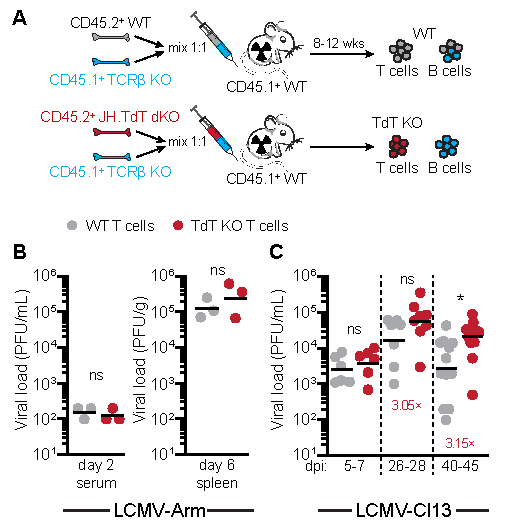
\includegraphics{Figures/AvC/fig5_tdtKO.pdf}
    \caption[Loss of TdT restricted to T cells in vivo impairs control of chronic, but not acute, infections]{\textit{Loss of TdT restricted to T cells in vivo impairs control of chronic, but not acute, infections}. %
    %
    \secbfcolor{(A)}~Generation of bone marrow chimeric mice possessing WT B~cells, and either WT T~cells (reconstitution of irradiated mice with 1:1 ratio of bone marrow from WT mice and TCR\textbeta{}\KO{} mice) or TdT KO T~cells (reconstitution with 1:1 ratio of bone marrow from JH and TdT double KO mice and TCR\textbeta{}\KO{} mice). %
    %
    \secbfcolor{(B)}~LCMV-Arm viral loads in the serum (left) and spleen (right) of mice with WT or TdT KO T cells measured at 2 or 6 days post-infection, respectively (n=3 mice per group). %
    %
    \secbfcolor{(C)}~LCMV-Cl13 viral loads in the serum of mice with WT or TdT KO T cells in early (5-7 days post-infection), mid (26-28 days post-infection) or late (40-45 days post-infection) stages of viral replication (n=6-18 mice per group). Fold-changes of viral loads in mice with TdT-deficient T cells, relative to WT, are indicated. *, P = 0.013 computed using a Kruskal-Wallis test.}
    \label{fig:AvC_tdtKO}
\end{figure}
%
We verified that our bone marrow reconstitutions led to a 1:1 ratio of hematopoietic cell development from each of the donors, identified using congenic markers (Fig.~\ref{fig:AvC_supp_tdtKO}A). In line with previous results from full TdT KO mice in response to acute LCMV infection~\cite{gilfillan1995efficient}, we observed no differences in the viral load following LCMV-Arm infection between the WT T cell and TdT KO T cell groups, both 2~days post infection in the serum, and 6 days post infection in the total spleen homogenate (Fig.~\ref{fig:AvC_tdtKO}B). In contrast, mice with TdT KO T~cells had a significantly higher viral load (3.15-fold increase) during the chronic phase (day 40-45) following infection with LCMV-Cl13 (Fig.~\ref{fig:AvC_tdtKO}C). Since irradiated bone marrow recipients still retain some endogenous hematopoietic stem cells, we repeated the above experiment using TCR\textbeta{} KO recipient mice instead (i.e., mice lacking endogenous \textalpha{}\textbeta{}T cells), and obtained similar results where chimeras with TdT KO T cells had a 3.74-fold increase in viral load by day~41 post-infection (Fig.~\ref{fig:AvC_supp_tdtKO}B-C).

Previous experimental and theoretical studies alike have shown that limiting the breadth of the T cell response to infection, or introducing “gaps” in the TCR repertoire, can impede pathogen control~\cite{meyer2004limited,van2011costimulatory,van2013rate}. We therefore wanted to investigate whether introducing similar gaps in the context of our pMHC-reactivity model could equally recapitulate the viral load data in mice with TdT KO T cells, demonstrating impaired chronic (but not acute) pathogen control. To test this, we constructed an alternative \dTCR{} repertoire where we decreased the number of T cell clonotypes 10-fold, without affecting the overall affinity profile or the total population size of the precursor pool (Fig.~\ref{fig:AvC_supp_alternativeKO}A). Interestingly, when we simulated both acute and chronic infections using this alternative \dTCR{} repertoire configuration, we found no differences in pathogen clearance in either case (Fig.~\ref{fig:AvC_supp_alternativeKO}B-C), inconsistent with what we saw in mice with TdT KO T~cells (Fig.~\ref{fig:AvC_tdtKO}). Incidentally, we also tested whether decreasing T cell precursor frequencies 10-fold instead (evenly across all pMHC-reactivity values) might recapitulate our experimental results, but again found a mismatch between the data and the simulations wherein acute, and not chronic, infection control seemed to be impaired relative to the WT configuration (Fig.~\ref{fig:AvC_supp_alternativeKO}D-F). Thus, while our modelling does not rule out the possibility for additional, affinity-independent advantages of TCR repertoire diversification by TdT, when taken together these results lend further support to notion that TdT benefits hosts challenged with chronic infections, and that it does so, at least in part, by generating T cells with lower affinity for foreign pMHC.



\section{Discussion}
\label{sec:AvC_discussion}

N-nucleotides added by TdT during V(D)J gene segment recombination contribute enormously to the diversification of the TCR repertoire~\cite{cabaniols2001most}. Yet, despite the fact that TdT is found in all jawed vertebrates with adaptive immune systems studied thus far~\cite{litman2010origins}, the specific contexts in which these non-germline TCRs are better poised to control pathogen replication have not been clear~\cite{gilfillan1995mice,gilfillan1995efficient}. Here we combined computational modelling and experimental approaches to investigate the temporal evolution of pMHC reactivities of responding T cells during infection and its impact on pathogen clearance. We developed a computational model that 1.~produced time courses characteristic of infections with both acute and chronic pathogens, and 2.~incorporated a continuum-affinity formalism to track T cell pMHC-reactivity distributions over time.  Using the \textit{in silico} model we developed, we made two predictions that we tested experimentally. First, we showed that, while in acute infection T cells with high pMHC reactivity predominate~\cite{busch1999t,bachmann1997functional,mcheyzer1995antigen}, during chronic infection T cells with low pMHC reactivity contribute disproportionately. Second, we found that the removal of low pMHC-reactivity T cells leads to a delay in chronic, but not acute, pathogen clearance in the model, which we replicated in infected mice when T cells were TdT-deficient. Importantly, our data corroborate prior experimental work showing no differences in clearance by TdT KO mice of the acute viral pathogens Vesicular Stomatitis, Sendai, Influenza A, and LCMV-WE~\cite{gilfillan1995efficient,haeryfar2008terminal}. Thus, while it has been proposed that a TdT-deficient TCR repertoire may have specific ‘holes’ with regard to antigen specificities represented, this has so far not been supported by experimental evidence. Indeed, without accounting for possible differences in T cell clonotype precursor frequencies, our model predicts longer times to clearance for chronic pathogens. Our work therefore suggests a hitherto undescribed benefit for TCR repertoire diversification by TdT in chronic infection control.

A TdT-deficient repertoire and its consequences for pathogen control are relevant not only for understanding the broad evolutionary conservation of TdT across vertebrates, but also in the context of neonatal immunity, given that the TCR repertoire is initially generated in the absence of TdT. TdT expression is first detected in thymocytes in mice and humans 3-5~days after birth and after 20 weeks of gestation, respectively~\cite{bonati1994tcr,bogue1992regulation}. Lacking N-nucleotide additions, neonatal TCR sequences are shorter, are more likely to be shared between individuals (public)~\cite{yassai2000thymocyte,yassai2002molecular} and are more cross-reactive~\cite{gavin1995increased}. Interestingly, in line with TdT KO T cells having greater pMHC reactivity, it has been shown that the neonatal repertoire is more self-reactive due to a greater affinity for pMHC, and neonatal T cells more prone to tolerance~\cite{rudd2020neonatal}. To what extent the neonatal TCR repertoire versus other epigenetic or transcriptional differences described in neonatal compared to adult T cells play a role in altered responses to infection requires further analysis.

Although we fit our model to viral replication data from acute and chronic strains of LCMV~\cite{wherry2003viral}, its conclusions may be generalizable to other pathogens. For instance, we found that following infection with the pulmonary fungal pathogen, C. neoformans, CD4\pos{} T cells with low self-pMHC reactivity, and thus low foreign reactivity~\cite{mandl2013t}, predominated among the responding effector T cells during the chronic infection phase. These experimental findings expand on previous work suggesting that, during chronic infection, T cells with lower pMHC-reactivity predominate in both CD4\pos{}~\cite{gallegos2016control} and CD8\pos{}~\cite{schober2020reverse,tsitsiklis2020unusual} T~cells. Notably, in our current model we did not distinguish between CD4\pos{} and CD8\pos{} T~cell responses, and it is possible that there are key differences between these T~cell subsets with regard to the role of TdT and functional biases among TdT-generated TCRs, which need to be further explored. Moreover, our model did not consider memory T cells following pathogen clearance, and experimental data suggests that memory T cells are differentially selected for in terms of their reactivity to pMHC, resulting in a final steady-state pMHC-reactivity distribution of memory T cells that differs from the starting na\"{i}ve T cell pMHC reactivity distribution~\cite{andargachew2018cd4,busch1999t,mandl2013t}. Of note, while our model does not include all aspects of the host-pathogen response, such as the effects of host age-related changes in T cell precursor sizes and responses, phenotypic complexities of different stages of T cell exhaustion, antigen abundance and immunodominance hierarchies, and pathogen evolution to evade host immunity~\cite{rouse2010immunity,mclane2019cd8,yewdell2006confronting}, the model could be extended by incorporating some of these additional phenomena in order to study their individual contributions to the control of acute or chronic pathogens in the context of a pMHC-reactivity continuum. Additionally, the effect of TdT deficiency in the B~cell receptor repertoire and its impact on acute or chronic pathogen clearance would be interesting to investigate in future studies.

Our work revealed the effects of varying features of the pMHC-reactivity distribution of responding T cells on pathogen clearance and suggested a differential role between T cells with low- and high-reactivity to pMHC during different phases of the immune response. This is particularly intriguing, given recent observations that in both mice and humans, both CD4\pos{} and CD8\pos{} T cells with lower self-pMHC reactivity (low CD5 surface levels) express higher levels of \textit{Dntt}, the gene encoding TdT~\cite{rogers2021pre,sood2021cd5,fulton2015tcr}. Thus, differences in TdT expression level during development in individual thymocytes may ultimately contribute to the numbers of N-nucleotides inserted into the recombining TCR and be a critical variable impacting strength of pMHC reactivity. To provide additional insight into whether there are indeed different roles for TdT-mediated versus germline-encoded TCRs during infection, comprehensive TCR sequencing studies will be a powerful tool. Indeed, recent work using machine learning has shown that CD4\pos{} T cells with higher self-pMHC-reactivity have fewer N-nucleotide additions on average when compared to T cells with lower reactivity to pMHC, and that longer TCR sequences with a greater number of N-nucleotide additions predominate in chronic infection~\cite{textor2022machine}. Overall, our model formalism provides a foundation for further studies of T cell pMHC-reactivity distributions over the course of an immune response, and it will be particularly interesting to investigate whether, as our model suggests, TdT-dependent TCRs are important in the control of other chronic pathogens and are perhaps making underappreciated contributions in settings such as cancer and autoimmunity.


\section{Materials and Methods}

\subsection{Mice}

C57BL/6, congenic CD45.1\pos{}, congenic Thy1.1\pos{}, and TCR\textbeta{}\KO{} mice~\cite{mombaerts1992mutations} were purchased from Jackson Laboratories (Bar Harbor, ME). The TdT\KO{} mice were shared by Dr. A. Feeney (The Scripps Research Institute)~\cite{gilfillan1993mice} and the JH\KO{} mice were shared by Dr. J. Fritz (McGill)~\cite{gu1993independent}. All mice were on a C57BL/6 background, bred in-house and experiments performed at 6-12 weeks of age with both males and females. Animal housing, care, and research were in accordance with the Guide for the Care and Use of Laboratory Animals and all procedures performed were approved by the McGill University Animal Care Committee.

\subsection{Pathogen stocks and infections}

\subsubsection{LCMV}

LCMV-Arm and -Cl13 strains were propagated from stocks provided by Dr. M. Richer (University of Indiana) on BHK-21 or L929 cells (ATCC). Briefly, virus was added at MOI 0.01, incubated for 90 minutes in serum-free media at 37\degree{C} in 5\% CO\sub{2}, then topped up with complete media for incubation for another 48 hours before harvesting the supernatant. BHK-21 cells were cultured in EMEM supplemented with 0.1\% penicillin/streptomycin, 1\% L-glutamine, 1\% non-essential amino acids, 1\% sodium pyruvate, and 10\% FBS and maintained at 37\degree{C} in 5\% CO\sub{2}. L929 cells were cultured in RPMI supplemented with 10\% FBS, 1\% L-glutamine, and 1\% penicillin/streptomycin. Mice were infected with 2\E{5} plaque forming units (PFU) of LCMV-Arm by intra-peritoneal injection or 2\E{6} PFU by intravenous injection for LCMV-Cl13 as previously described~\cite{wherry2003viral,richer2013pathogen}. Mice were bled by either tail artery or cardiac puncture into sterile Eppendorf tubes kept on ice, blood was spun down at 12,000 rpm for 10 minutes and serum aliquoted and frozen for viral titer determination. Spleens were collected in 1\% RPMI and weighed. Spleens were placed in Lysing Matrix D tubes (MP Biomedicals) and homogenized with a MagNA Lyser (Roche) at 6000 rpm for 40 seconds. Spleen homogenate was then spun down at 12,000 rpm for 10 minutes at 4\degree{C} and supernatant was transferred to a separate sterile tube and re-spun at 12,000 rpm for 10 minutes at 4\degree{C} then aliquoted and frozen for viral titer determination. Viral titers (stocks used, mouse serum, and tissue samples) were determined by plaque assay with Vero cells~\cite{ahmed1984selection}. Briefly, Vero cell monolayers were infected with 100 \textmu{}L of serially diluted serum (1 in 10 dilutions from $10^{-1}$ to $10^{-7}$) and incubated for 90~minutes at 37\degree{C} in 5\% CO\sub{2}. Infected cells were then overlaid with 1\% agarose (Wisent) and incubated for 3 days at 37\degree{C} in 5\% CO\sub{2}. A second agarose overlay supplemented with 1\% neutral red was then added and cells incubated for 24~hours at 37\degree{C} in 5\% CO\sub{2}, after which plaques were counted.

\subsubsection{\textit{C. neoformans}}

The H99 strain was provided by K. Kwon-Chung (NIH). Frozen stocks ($-80$\degree{C}) were prepared in 15\% glycerol from fresh cultures from a YPD agar plate. Three days before infection, \textit{C. neoformans} was scraped from the frozen stock and streaked onto a YPD agar plate. One day prior to infection, a single colony was inoculated and incubated for 12-16 hours at 30\degree{C} with continuous agitation in YPD broth. Immediately before infection, \textit{C. neoformans} was resuspended in cold PBS. Mice were then anesthetized with isoflurane and infected by intrapharyngeal aspiration with 5\E{3} colony forming units (CFU) in 20 \textmu{}L of PBS. Mice were sacrificed and tissue collected 23 days after infection. \textit{C. neoformans} CFUs were determined as previously described~\cite{schneider2020migration}.

\subsection{Lymphocyte isolation}

For the C. neoformans infections, prior to harvest an intravascular stain using 2.5 µg anti-CD45 (30F11) was performed as previously described (62). Infected lungs were harvested in cold PBS and minced with scissors. Lung was then digested at 37\degree{C} with agitation for 30 minutes in digestion buffer (1~mg/mL collagenase D, 50~U/mL DNase I, 1~mg/mL hyaluronidase, 1\% L-glutamine, 1\% pen/strep in RPMI). Tissue was then passed through a 100-μm filter with PBS supplemented with 1\% FBS and resuspended in 10~mL of 37\% Percoll in RPMI. Samples were centrifuged at 3000~rpm for 20~minutes at 22\degree{C}. ACK lysis buffer (Life Technologies) was added for 3~minutes, samples washed with PBS, refiltered, and resuspended in complete RPMI (10\% FBS, 1\% L-glutamine, 1\% HEPES buffer, 1\% pen/strep, 1\% sodium pyruvate, 1\% non-essential amino acids, 0.1\% 2-mercapto-ethanol 1000X solution). Dilution of single-cell suspensions at 1:10 in Trypan Blue and manual counting of live cells (Trypan Blue-negative) on a hemacytometer was used to determine total cell counts.

Spleen and peripheral lymph nodes (inguinal, axillary, brachial, and mesenteric) were collected and passed through a 70-μm filter with 1\% RPMI (1\% penicillin/streptomycin, 1\% L-glutamine, and 1\% FBS). ACK lysis buffer (Life Technologies) was added for 3 minutes, samples washed with PBS, refiltered and resuspended in 1\% RPMI. Dilution of single-cell suspensions at 1:10 in Trypan Blue and manual counting of live cells (Trypan Blue-negative) on a hemacytometer was used to determine total cell counts.

\subsection{Bone marrow chimeras}

Bone marrow was collected from the femurs and tibias of donor mice (either JH\KO{} TdT\KO{}, TCR\textbeta{}\KO{}, or B6 WT) by flushing the marrow from the bones with cold 1\% RPMI. Bone marrow cells were then passed through a 70~\textmu{}m filter with 1\% RPMI and red blood cells lysed with ACK lysis buffer (Life Technologies) and cell counts determined as above. Recipient mice (either B6 CD45.1\pos{} or TCR\textbeta{}\KO{} CD45.1\pos{}) were irradiated twice at 550 rads 3 hours apart and reconstituted with a 1:1 mix of 2.5\E{6} cells per genotype that were injected intravenously within 5 hours of the first irradiation. To establish the WT chimera (WT T cells and B cells) B6 and TCR\textbeta{}\KO{} bone marrow cells were mixed at equal proportions; to make the T cell restricted TdT\KO{} chimeras (WT B cells) bone marrow cells from JH\KO{} TdT\KO{} mice were mixed 1:1 with TCR\textbeta{}\KO{} bone marrow cells. Recipient mice were given neomycin water (2~g/L) 2 days prior to bone marrow transfer and kept on the antibiotic water for 2~weeks following transfer. Mice were used 8-12~weeks post irradiation and bone marrow reconstitution.

\subsection{Flow cytometry}

Samples were incubated in Fixable Viability Dye (AF780, Life Technologies) diluted in PBS for 20 minutes at 4\degree{C}. Extracellular antibodies were diluted in FACS buffer (2\% FBS and 5~mM EDTA in PBS) with Fc Block (Life Technologies) and incubated for 30 minutes at 4\degree{C}. For intracellular staining, samples were then incubated in FoxP3 Transcription Factor Fixation/Permeabilization Concentrate and Diluent (Life Technologies) for 30~minutes at 4\degree{C}. Intracellular antibodies were diluted in Permeabilization Wash Buffer (Life Technologies) and samples were incubated for 30-60 minutes at 4\degree{C}. Directly conjugated antibodies used were as follows: TCRb (H57-597), CD4 (RM4.5), CD8a (53-6.7), CD5 (53-7.3), Foxp3 (FJK-16 s), CD44 (IM7), CD62L (MEL-14), CD25 (PC61.5), CD45.1 (A20), CD45.2 (104), PD-1 (29F.1A12), B220 (RA3-6B2), NK1.1 (PK126). For all flow cytometry experiments, cells were acquired using an LSRFortessa (BD Bioscience) and analyzed with FlowJo software (BD Bioscience).

\subsection{Cell sorts}

Cell sorts were performed as previously described~\cite{rogers2021pre}. Briefly, lymphocytes from Thy1.1\pos{} or CD45.1\pos{} congenic mice were isolated in single cell suspension as described. Spleens and lymph nodes (inguinal, axially, brachial, mesenteric, and cervical) were pooled from 15 mice for each congenic marker. Cells were then magnetically enriched for total CD4+ T cells (Stemcell EasySep CD4\pos{} T cell Enrichment kit or Miltenyi Biotec CD4\pos{} T cell Isolation Kit). Enriched CD4\pos{} T cells were stained with surface antibodies for 1~hour at 4\degree{C}. Naive CD4\pos{} T cells were sorted on singlets, CD4\pos{}, CD8\neg{}, CD62L\supr{hi}, CD44\supr{lo}, and 20\% CD5\supr{hi} or CD5\supr{lo}. Sorts were performed on a FACS Aria III (BD Bioscience). All cell populations were sorted to $>$90\% purity.

\subsection{Adoptive cell transfers}

\textit{C. neoformans} infection. All donors and recipients were sex matched. 15 CD45.1\pos{} or Thy1.1\pos{} mice were used as donors to obtain a total of 8-14\E{6} cells for each of 20\% CD5\supr{hi} and 20\% CD5\supr{lo} cells sorted as described above. Sorted CD5\supr{lo} and CD5\supr{hi} were then mixed in a 1:1 ratio. 4-7\E{6} of each sorted population was adoptively transferred into CD45.2\pos{} Thy1.2\pos{} recipients that were infected with 5\E{3}~CFU of \textit{C. neoformans} 3 days prior to transfer. Cells were isolated from the lungs of recipient mice 20 days post-transfer.

\subsection{Statistical analyses of experimental data}

Group comparisons were performed using Prism V9 (GraphPad). The cut-off for significance considered was p$<$0.05. Information about implemented statistical tests and sample sizes for individual experiments is provided in the figure legends.

\subsection{Computational modelling}

To study a continuum of antigen-specific T cell affinities in the context of acute vs. chronic pathogen infections, we used the following system of integro-differential equations based on Fig.~\ref{fig:AvC_scheme}:
%
\begin{align}
    \dv{P}{t} &= r_P P \left( 1 - \frac{P}{P_{\textrm{max}}}\right) - \kappa_P \int_{\kmin{}}^{\kmax{}} E(t,k) \frac{P}{P+a \, k} \, \dd k \label{eq:AvC_P} \\[0.3em]
    \begin{split}
        \pdv{E(t,k)}{t} &= \sigma_E(k) + r_E E(t,k) \frac{P}{P+k} - \delta_E E(t,k) \\
        &\quad- \kappa_E E(t,k) \frac{P}{P+b\,k} - \varepsilon E(t,k) \int_{\kmin{}}^{\kmax{}} E(t,k) \dd k
    \end{split} \label{eq:AvC_E}
\end{align}
%
This was implemented in a manner similar to the models presented in~\cite{jamaleddine2020quantifying,jaberi2015continuum}. In Eqs.~\eqref{eq:AvC_P} and~\eqref{eq:AvC_E}, $P(t)$ represents the pathogen load in time, and $E(t,k)$ represents the time-dependent reactivity-continuum of effector T cells, with T cell pMHC reactivity taken to be proportional to the quantity $1/k$, where $k$ is the pathogen load for half-maximum activation of T cells. To facilitate understanding of pMHC-reactivity distributions, we defined a new, unitless quantity $a_k$ (whose magnitude is equivalent to $1/k$) as a measure for T cell reactivity to pMHC~\cite{standifer2009changes}. While this quantity is related to the overall binding avidity between T cells and APCs, we considered only affinity-related changes in TCR binding strength, and thus used the term pMHC reactivity to avoid confusion with other factors that can affect binding avidity. For simplicity, in Eq.~\eqref{eq:AvC_P} we assumed a logistic growth of the pathogen (with replication rate $r_P$ and carrying capacity $P_\textrm{max}$) as was done in previous models of LCMV infection~\cite{bocharov1998modelling,kecsmir2003clonal}. Clearance of the pathogen by T cells was described by a product of the T cell number ($E$) and an increasing first-order Hill function of pathogen load with a maximum rate $\kappa_P$, and a half-maximum pathogen load $a \cdot k$ (where $a$ is a scaling factor). We impose the condition that the pathogen replication rate ($r_P$) for chronic pathogens to be larger than that for acute pathogens, as suggested previously in the case of LCMV-Cl13 vs. LCMV-Arm, respectively~\cite{bergthaler2010viral,sullivan2011point}.

The terms included in effector cell dynamics of Eq. 2 were pMHC reactivity-dependent thymic input ($\sigma_E(k)$), T cell replication that depends on pathogen load according to a first-order Hill function (with maximum replication rate $r_E$ and half-maximum activation $k$), natural turnover (with a rate $\delta_E$), and an inter-cellular competition term (with a rate $\varepsilon$). The parameter $\kappa_E$ denotes the rate at which the pathogen causes reduction in the number of active effector T cells able to provide anti-microbial immunity, either via T cell exhaustion, activation-induced cell death, or regulatory T cell intervention. The term $b \cdot k$ represents the pathogen load at half the maximum inactivation rate of effector T cells, where $b>1$ is a proportionality constant.

To study the effects of T cell reactivity to pMHC in the context of acute vs. chronic infection, we denoted the spectrum of effector T cells in time by $E(t,k)$, where $k=1/a_k$ is assumed to be proportional to the reciprocal of T cell reactivity to pMHC consistent with~\cite{standifer2009changes}, $\kmax{}$ is the maximum value of $k$ (corresponding to T cells with the lowest reactivity to pMHC) and $\kmin{}$ is the minimum value of $k$ (corresponding to T cells with highest reactivity to pMHC). Equations~\eqref{eq:AvC_P} and~\eqref{eq:AvC_E} are simulated by discretizing the allowable values of pMHC reactivity within the range defined by $1/\kmax{}$ and $1/\kmin{}$, wherein the solution is obtained by integrating a high-dimensional system of ordinary differential equations (see Section~\ref{sec:AvC_numericalSimmulation}).

\subsection{Model parameters and numerical implementation}
The two pMHC reactivity dependent parameters, $\sigma_E$ and $\kappa_E$, were defined to be functions of T cell reactivity to pMHC ($a_k$) (Fig.~\ref{fig:AvC_scheme}B,~C). A bell-shaped function of pMHC reactivity that mimics a log-normal distribution was used to assign values for thymic input $\sigma_E$, while T cell exhaustion $\kappa_E$ was first sampled from an exponential distribution and then sorted in an ascending order (such that higher-affinity T cells are more susceptible to losing their effector functions than their lower-affinity counterparts). This latter claim is supported by the fact that activation-induced cell death~\cite{alexander1996role} and T cell exhaustion~\cite{wherry2003viral,shakiba2021tcr} scale with the strength of antigenic stimulation. The use of a uniform distribution for $\kappa_E$ produced very similar results (Fig.~\ref{fig:AvC_supp_uniformExhaustion}). Table~\ref{tab:AvC_parameters} summarizes the meanings of the different parameters and their values used to generate model results. Model parameters were obtained by genetic algorithm fitting to LCMV-Arm and LCMV-Cl13 serum data adapted from~\cite{wherry2003viral} (Fig.~\ref{fig:AvC_supp_timeSeries}A-B). To simulate the \dTCR{} repertoire shown in Fig.~\ref{fig:AvC_modelKO}C, the thymus input parameter $\sigma_E$ was modulated by an arctan function such that
%
\begin{equation*}
    \sigma_E^{\textrm{\dTCR{}}}(k) = \frac{1}{2} \sigma_E(k) \left[ 1 - \arctan\left( \frac{\log_{10}k - \log_{10}\kmode{}}{0.15} \right) \right],
\end{equation*}
%
where $\kmode{}$ is the value of the parameter $k$ at which $\sigma_E(k)$ peaks, determined by parameter fitting (for more details, see Section~\ref{sec:AvC_modelParsFitting} - Model parameters and fitting). The new parameter $\sigma_E^{\textrm{\dTCR{}}}(k)$ is subsequently renormalized such that the total thymic input across all T cells remains constant, i.e.,
%
\begin{equation*}
    \sigma_E^{\textrm{\dTCR{}}}(k) \rightarrow \sigma_E^{\textrm{\dTCR{}}}(k) \left( \int_{\kmin{}}^{\kmax{}} \sigma_E (k) \, \dd k \right) \Big/ \left( \int_{\kmin{}}^{\kmax{}} \sigma_E^{\textrm{\dTCR{}}}(k) \, \dd k \right).
\end{equation*}

MATLAB was used to simulate the model equations and perform numerical analyses. Steady state and bifurcation analyses were carried out using XPP/AUTO, a freeware available at \url{http://www.math.pitt.edu/~bard/xpp/xpp.html}). Genetic algorithm fitting was performed using Compute Canada’s Cedar cluster. MATLAB codes used to produce violin plots are available at \url{http://github.com/bastibe/Violinplot-Matlab}. All other MATLAB codes used to perform simulations, parameter fitting, and model analyses can be obtained online at \url{http://www.medicine.mcgill.ca/physio/khadralab/Codes/code_PNAS1.html}.


\section{Acknowledgments}

This work was done in Tiohtiá:ke/Montreal on the traditional territory of the Kanien’kehà:ka, a place which has long served as a site of meeting and exchange amongst many First Nations including the Kanien’kehà:ka of the Haudenosaunee Confederacy, Huron/Wendat, Abenaki, and Anishinaabeg. We honour, recognize, and respect these nations as the traditional stewards of these lands and waters. We would like to thank the animal facility staff at McGill University for their excellent care of our animal colony, C. Stegen and J. Leconte at the Cell Vision Core Facility for cell sorting, F. Buytenhuijs and J. Textor at Radboud University for key intellectual input and for conducting separate analyses not included in the paper, and P. Artusa for initial experiments at an earlier stage of the project that were also not included. H.J. was supported by a Post-Graduate Doctoral Award (NSERC) and a B2X Doctoral Award (FRQNT). D.R. was supported by a Frederick Banting and Charles Best Canada Graduate Doctoral Award (CIHR) and a Tomlinson Doctoral Fellowship (McGill). J.N.M. is a Canada Research Chair for Immune Cell Dynamics. This work was supported by NSERC (Discovery Grants \#2019-04520 to A.K. and \#2016-03808 to J.N.M.).

\newpage
\section{Supporting information}

\renewcommand{\thetable}{S\thechapter.\arabic{table}}
\setcounter{table}{0}

\subsection{Supplementary tables and figures}

Table~\ref{tab:AvC_parameters}, supporting figures, legends for supporting movies, and supporting text are included below. Video files for the supporting movies may be downloaded from the manuscript preprint in~\cite{jamaleddine2022chronic}.

\vspace{0.5in}

\begin{table}[ht]
\footnotesize
\centering
\begin{tabular}{p{0.06\textwidth} p{0.53\textwidth} p{0.12\textwidth} p{0.17\textwidth}}
    \hline
    \textbf{Param.} & \textbf{Description}                                             & \textbf{Value(s)} & \textbf{Units} \\
    \hline
    %
    $r_P$ & Maximum pathogen replication rate & 0.77 (acute) & day$^{-1}$ \\
    & & 1.22 (chronic) & \\
    %
    $P_0$ & Initial pathogen load & 28.4 (acute) & PFU~mL$^{-1}$ \\
    & & 98.3 (chronic) & \\
    %
    $P_{\textrm{max}}$ & Pathogen carrying capacity & 1.17\E{5} & PFU~mL$^{-1}$ \\
    %
    $\kappa_P$ & Maximum pathogen removal rate per T cell & 4.94\E{-2} & PFU~(mL~cell~day)$^{-1}$ \\
    %
    $k$ & Pathogen load at half-maximum activation of T cells & Range & PFU~mL$^{-1}$ \\
    %
    $a_k$ & pMHC reactivity parameter (magnitude equal to $1/k$) & Range & unitless \\
    %
    $a$ & Scaling factor of half-maximum constant in pathogen clearance & 1.77\E{-3} & unitless \\
    %
    $\sigma_{E,\textrm{tot}}$ & Total thymic input across all pMHC-reactivity values & 29.7 & cells~day$^{-1}$\\
    %
    $k_{\textrm{mode}}$ & Mode of the pMHC-reactivity function at which thymic input is maximal &  7.8\E{2} & PFU~mL$^{-1}$ \\
    %
    $k_{\textrm{span}}$ & Span of the pMHC-reactivity function & 1.91 & unitless \\
    %
    $r_E$ & Proliferation rate of effector T cells & 3.19 & day$^{-1}$ \\
    %
    $\delta_E$ & Natural turnover rate of effector T cells & 0.28 & day$^{-1}$ \\
    %
    $\kappa_E$ & Pathogen-dependent T cell exhaustion rate - sampled from a shifted exponential distribution $g(k;\mu) + \kappa_{E,\textrm{min}}$ and sorted (highest $a_k$ corresponds to highest $\kappa_E$ value) & $\mu$ = 3.34 & day$^{-1}$ \\
    %
    $\kappa_{E,\textrm{min}}$ & Minimum exhaustion rate & 0.39 & day$^{-1}$ \\
    %
    $b$ & Scaling factor of half-maximum constant of T cell exhaustion & 38.1 & unitless \\
    %
    $\varepsilon$ & Inter-cellular competition rate & 3.24\E{-6} & cell$^{-1}$~day$^{-1}$ \\
    %
    $N$ & Number of T cell clones obtained from discretizing Eqs.~\eqref{eq:AvC_P}-\eqref{eq:AvC_E} (see Section~\ref{sec:AvC_numericalSimmulation} -- Numerical simulation) & 500 & unitless \\
    \hline
\end{tabular}
\caption[Parameter values used in model simulations]{\textit{Parameter values used in model simulations}. Values were determined by fitting model simulations to serum data in acute vs. chronic LCMV infection~\cite{wherry2003viral} using a genetic algorithm.}
\label{tab:AvC_parameters}
\end{table}

\renewcommand{\thefigure}{S\thechapter.\arabic{figure}}
\setcounter{figure}{0}

% Movies
\vspace{0.5in}
\begin{figure}[h]
    \centering
    \captionsetup{name={Movie}}
    \caption[]{\secbfcolor{(A-F)}~Time series simulations of the model during acute (A-C) or chronic (D-F) infection, showing pathogen loads (A,~D), heat maps representing the relative proportion of T cells across pMHC reactivities (B,~E), and evolution of T cell proportions as a function of pMHC reactivity at each time point (C,~F). Overlaid traces in B and E represent the mean reactivity value in time, weighted by the proportion of T cells of given reactivity values. Dotted black lines denote the time at which the pathogen is cleared.}
    \label{mov:AvC_timeSeries}
\end{figure}

\begin{figure}
    \centering
    \captionsetup{name={Movie}}
    \caption[]{\secbfcolor{(A-B)}~Nullclines of the reduced, 2-dimensional, one-clone model plotted in logarithmic (A) and linear (B) scales over time during chronic pathogen replication. Nullclines vary over time since the parameters for pMHC reactivity ($a_k$) and exhaustion rate ($\kappa_E$) of the one-clone model were set to their respective weighted average values across all T cells of the full model at each time point. Given that the relative proportions of T cells of different pMHC reactivity values vary through time in the full model, the weighted averages of these parameters also change over time. Black lines represent pathogen load ($P$) nullclines while the gray line represents the effector T cell ($E$) nullcline. Superimposed in green is the pathogen load and the total T cell count (across all values of pMHC reactivity) simulated from the full model across time. Refer to Section~\ref{sec:AvC_2DmodelAnalysis} - Analysis of the reduced one-clone, 2D model for more details.}
    \label{mov:AvC_nullclines}
\end{figure}

\renewcommand{\thefigure}{S\thechapter.\arabic{figure}}
\setcounter{figure}{0}

\begin{figure}[htbp]
    \centering
    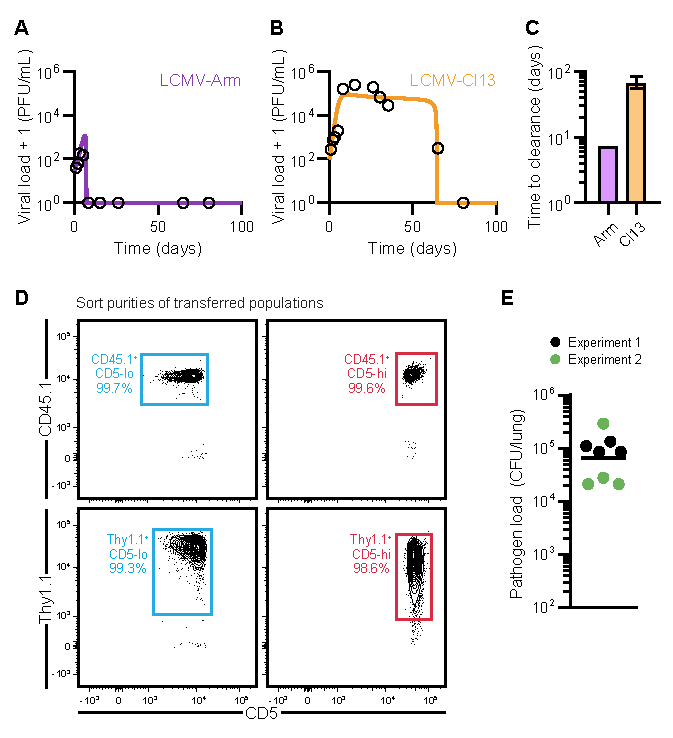
\includegraphics[width=0.64\textwidth]{Figures/AvC/figS1_timeSeries.pdf}
    \caption[Model fitting and adoptive cell transfer experiment set-up details]{\textit{Model fitting and adoptive cell transfer experiment set-up details}. %
    %
    \secbfcolor{(A,~B)}~Serum viral load data in mice infected with LCMV-Arm (A) or LCMV-Cl13 (B) digitized from~\cite{wherry2003viral}, shown as open circles, overlaid on the time series simulations of Eqs.~\eqref{eq:AvC_P}-\eqref{eq:AvC_E}. These simulations were generated using parameter values (Table~\ref{tab:AvC_parameters}) obtained from fitting the model to digitized data shown in (A) and (B) with the implementation of the genetic algorithm (see Section~\ref{sec:AvC_modelParsFitting} - Model parameters and fitting for details). Note that the difference between the two curves was generated by altering the pathogen replication rate parameter and initial pathogen load. %
    %
    \secbfcolor{(C)}~Median time to clearance of 100 simulations for acute and chronic infections (error bars = 95\% confidence intervals). %
    %
    \secbfcolor{(D)}~Flow cytometry panels showing sort purities of transferred CD45.1\pos{} or Thy1.1\pos{} CD5\supr{lo} and CD5\supr{hi} na\"{i}ve CD44\supr{lo} CD62L\pos{} CD4\pos{} T~cells into \textit{C. neoformans} infected mice. %
    %
    \secbfcolor{(E)}~\textit{C.~neoformans} pathogen loads in the lungs of infected mice from 2 independent experiments (n=8 mice).}
    \label{fig:AvC_supp_timeSeries}
\end{figure}

\begin{figure}
    \centering
    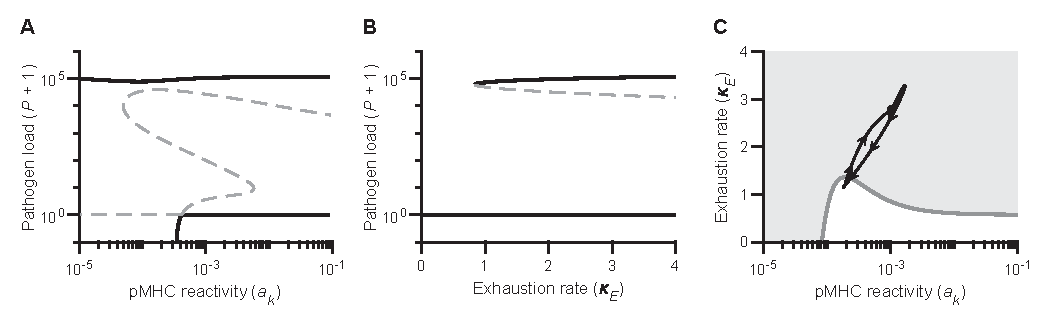
\includegraphics[width=\textwidth]{Figures/AvC/figS2_bfns.pdf}
    \caption[Bifurcation analysis of the one-clone system]{\textit{Bifurcation analysis of the one-clone system}. %
    \textbf{(A)}~Pathogen levels at steady state as a function of pMHC reactivity ($a_k=1/k$); solid black lines represent branches of attracting (stable) equilibria, while dashed lines represent branches of repelling (unstable) equilibria. The upper and lower levels of pathogen load can coexist (in the form of bistability) in the upper range of pMHC reactivity; which one of these two steady states can be attained depend on the initial conditions of pathogen load and T cell count. %
    %
    \textbf{(B)}~Pathogen levels at steady state as a function of the pathogen-dependent effector T cell depletion, $\kappa_E$, when $a_k=10^{-2.98}$; as before, solid black lines represent branches of attracting (stable) equilibria, while dashed lines represent branches of repelling (unstable) equilibria. %
    %
    \textbf{(C)}~Two-parameter bifurcation of steady state level of pathogen load with respect to the depletion rate $\kappa_E$ and pMHC reactivity parameter, $a_k$. Gray-shaded region represents the regime of coexistence between the upper and lower levels of pathogen load (i.e., the bistable regime) seen in (A) and (B). Overlaid is the trajectory of the average pMHC reactivity and average depletion rate of the ensemble of T cells of the full system, starting from the filled black circle (arrows indicate direction of motion).}
    \label{fig:AvC_supp_bfns}
\end{figure}

\begin{figure}
    \centering
    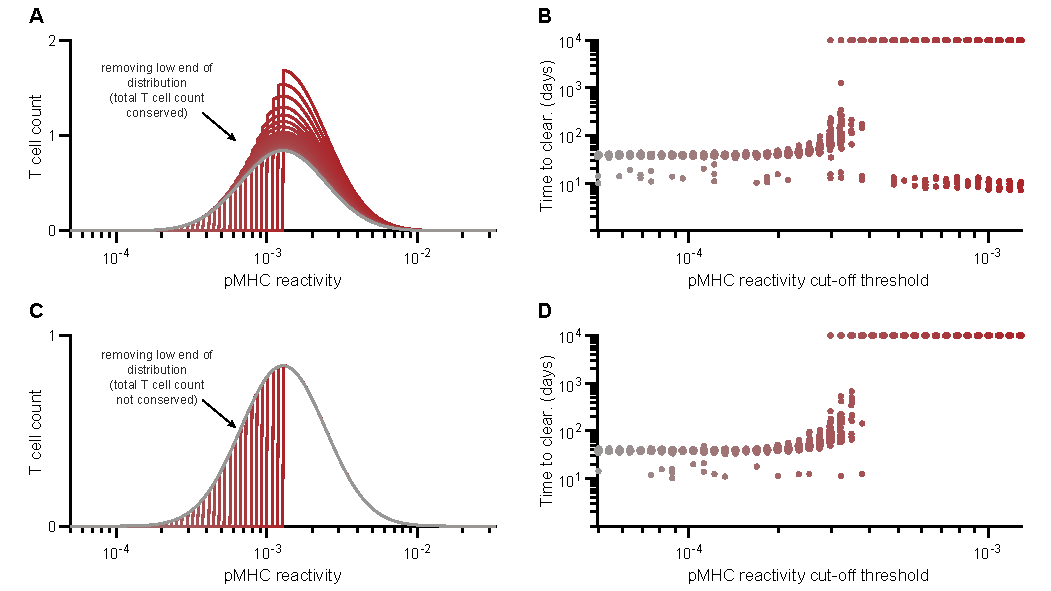
\includegraphics[width=\textwidth]{Figures/AvC/figS3_modelKO.pdf}
    \caption[Effects of removing T cells with low pMHC-reactivity]{\textit{Effects of removing T cells with low pMHC-reactivity}. %
    %
    \secbfcolor{(A)}~Distributions of initial T cell count prior to infection as a function of pMHC reactivity obtained by successively removing low-reactivity T cells using different cut-off thresholds from the model’s pre-infection repertoire and by reducing the pathogen replication rate $r_P$ to 1.16~day$^{-1}$ from its default value. Note that, since reducing $r_P$ does not affect the initial T cell count, these distributions are identical to those shown in Fig.~\ref{fig:AvC_modelKO}. %
    %
    \secbfcolor{(B)}~Time to pathogen clearance as a function of the cut-off threshold for T cell reactivity shown in (A). For each cut-off threshold, 50 simulation trials were performed as described in Fig.~\ref{fig:AvC_modelKO}. Notice the prominence of the acute cluster at high cut-off thresholds owing to a greater number of T cells with high pMHC reactivity; interestingly, this feature is not present in Fig.~\ref{fig:AvC_modelKO}B. %
    %
    \secbfcolor{(C)}~Distribution of T cell count prior to infection and with $r_P$ reduced to 1.16~day$^{-1}$, without keeping the total number of T cells conserved when removing the low-reactivity T cells at different cut-off thresholds. %
    %
    \secbfcolor{(D)}~Time to clearance as a function of the cut-off threshold of the pMHC reactivity shown in (C). Notice the disappearance of the acute cluster seen in (B) at high cut-off threshold values.}
    \label{fig:AvC_supp_modelKO}
\end{figure}

\begin{figure}
    \centering
    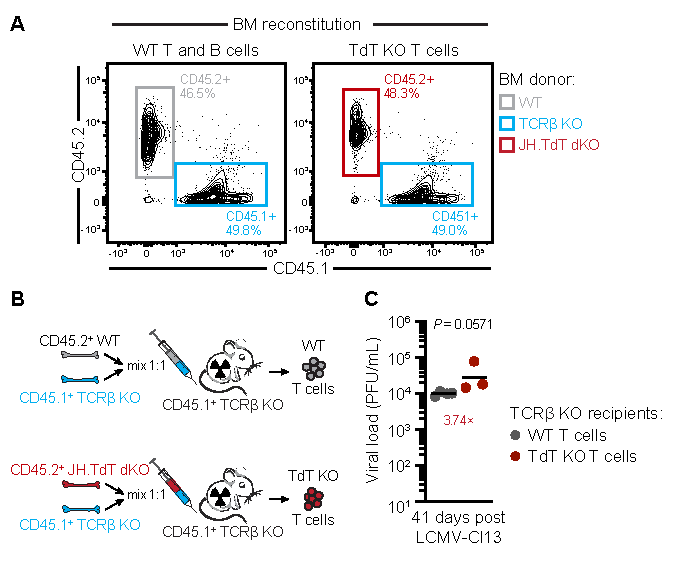
\includegraphics[width=0.64\textwidth]{Figures/AvC/figS4_tdtKO.pdf}
    \caption[Generating bone marrow chimeric mice lacking TdT in T cells only]{\textit{Generating bone marrow chimeric mice lacking TdT in T cells only}. %
    %
    \secbfcolor{(A)}~Representative flow cytometry plots showing the percent of bone marrow cells from each set of donor mice, namely CD45.1\pos{} cells from TCR\textbeta{} KO mice and CD45.2\pos{} cells from either WT or JH$\times$TdT double KO mice. %
    %
    \secbfcolor{(B)}~Modified experimental approach from Fig.~\ref{fig:AvC_tdtKO} by using TCR\textbeta{} KO mice as irradiated bone marrow recipients. %
    %
    \secbfcolor{(C)}~LCMV-Cl13 viral loads in the serum of recipient TCR\textbeta{}\KO{} mice reconstituted with WT or TdT KO T cells at day 41 post infection. P-value indicated was computed using two-tailed Wilcoxon rank sum test on geometric means.}
    \label{fig:AvC_supp_tdtKO}
\end{figure}

\begin{figure}
    \centering
    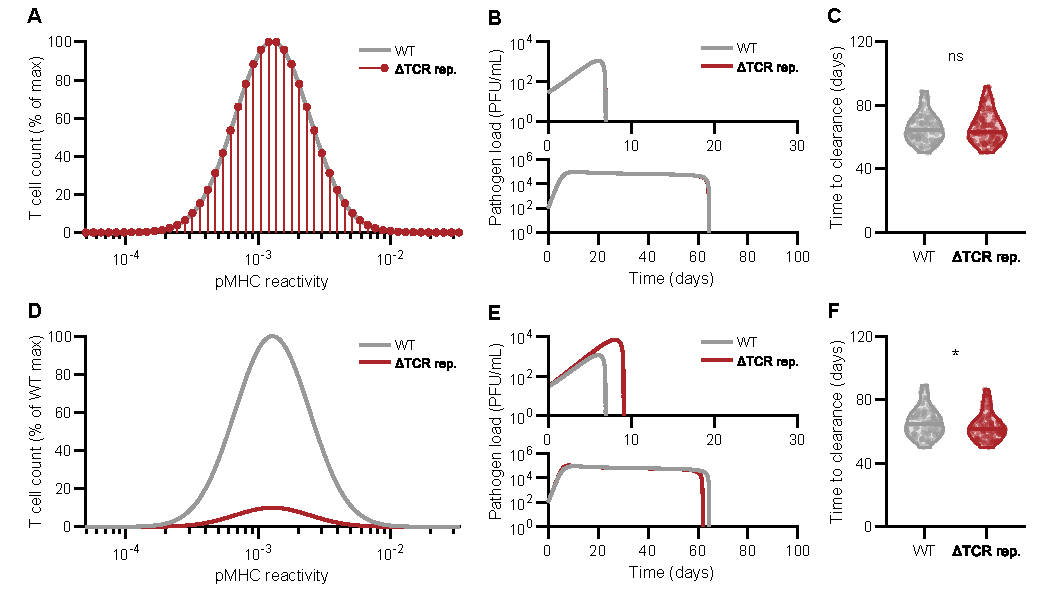
\includegraphics[width=\textwidth]{Figures/AvC/figS5_alternativeKO.pdf}
    \caption[Alternative changes to the TCR repertoire in the model produce outcomes that do not match the data in mice with TdT-deficient T cells]{\textit{Alternative changes to the TCR repertoire in the model produce outcomes that do not match the data in mice with TdT-deficient T cells}. %
    %
    \secbfcolor{(A,~D)}~Altered TCR repertoire obtained by either reducing the number of clonotypes by decreasing $N$ to 50, resulting in fewer clones across the entire pMHC reactivity range while keeping the total T cell count constant (A), or reducing precursor frequency across all pMHC reactivity values by decreasing $\sigma_{E,\textrm{tot}}$ 10-fold to 2.97 cells~day$^{-1}$ (D). %
    %
    \secbfcolor{(B,~E)}~Model simulations comparing representative pathogen load traces of WT (gray) and \dTCR{} repertoires (red) configurations in in A and C during acute (top) or chronic (bottom) infection when the number of clones is reduced (B) or when precursor frequencies are reduced (E). %
    %
    \secbfcolor{(C,~F)}~Time to clearance of chronic infections for 100 model simulations from WT and \dTCR{} repertoire systems associated with reducing number of clones (C) or precursor frequencies (F). ns, P = 0.78; *, P = 0.036. P-values computed using the Wilcoxon rank sum test.}
    \label{fig:AvC_supp_alternativeKO}
\end{figure}

\begin{figure}
    \centering
    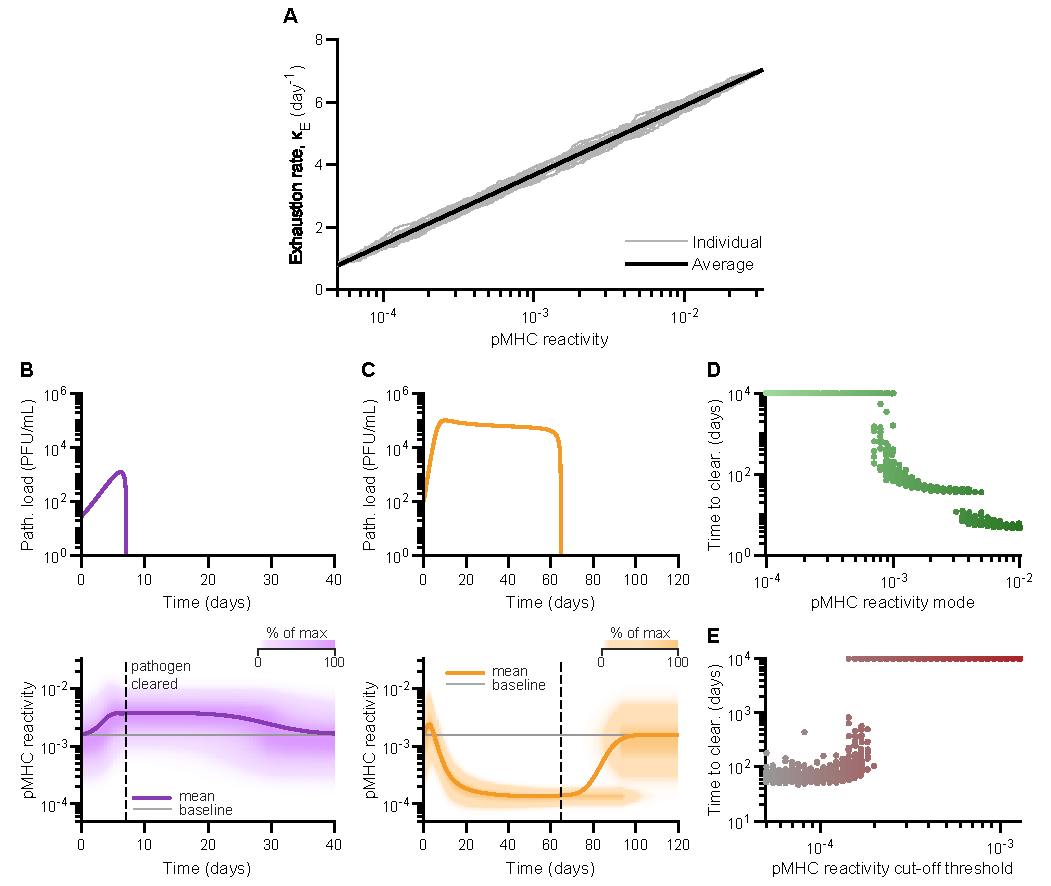
\includegraphics[width=\textwidth]{Figures/AvC/figS6_uniformExhaustion.pdf}
    \caption[Exhaustion rates sampled from a uniform distribution do not qualitatively alter model results]{\textit{Exhaustion rates sampled from a uniform distribution do not qualitatively alter model results}. %
    %
    \secbfcolor{(A)}~Function depicting pMHC reactivity-dependent exhaustion rate, $\kappa_E$, when sampling from a uniform distribution (with a lower bound of $\kappa_{E,\textrm{min}}$ as in Table~\ref{tab:AvC_parameters}, and upper bound $\kappa_{E,\textrm{max}}$ set to 6.67~day$^{-1}$) and sorting in ascending order. %
    %
    \secbfcolor{(B,~C)}~Pathogen load (top) and pMHC-reactivity distribution (bottom) obtained by simulating the model response to acute (B) or chronic (C) pathogen, when $\kappa_E$ was sampled from uniform distribution. Chronic replication rate ($r_P$) was reduced to 1.15~day$^{-1}$; all other parameters were kept at their default values shown in Table~\ref{tab:AvC_parameters}. %
    %
    \secbfcolor{(D,~E)}~Effect of varying the pMHC-reactivity mode (D), as in Fig.~\ref{fig:AvC_dists}A, or of removing T cells with low pMHC-reactivity (E), as in Fig.~\ref{fig:AvC_modelKO}B, when $\kappa_E$ was sampled from uniform distribution. Note that all results are consistent with those obtained by sampling $\kappa_E$ from an exponential distribution as shown in Fig.~\ref{fig:AvC_scheme}C.}
    \label{fig:AvC_supp_uniformExhaustion}
\end{figure}

\clearpage
\clearpage

\subsection{Model parameters and fitting}
\label{sec:AvC_modelParsFitting}

In order to generate parameter values for model simulations, a genetic algorithm was used. The fitness function of the genetic algorithm was primarily based on minimizing the sum of squared errors between the data and model predictions (i.e., minimizing $\sum_i(\mathbf{Y}_i-F(t;\mathbf{P}))^2$ , where $\mathbf{Y}_i$ is the serum time series data in~\cite{wherry2003viral}, and $F(t;\mathbf{P})$ is the fit output as a function of time with input parameter vector $\mathbf{P}$). The results were then refined to ensure the final selected parameter values satisfied the following conditions:
\begin{itemize}
    \item The pathogen replication rate for chronic LCMV (LCMV-Cl13) is larger than that for acute LCMV (LCMV-Arm), as suggested by~\cite{bergthaler2010viral,sullivan2011point}
    \item Pathogen load starts from a perturbed initial value $P_0$ (a fitted parameter, see below), and the rate of change of pathogen is initially positive i.e., $\textrm{d}P/\textrm{d}t>0$ at $t=0$.
    \item The steady state of the pathogen-free equilibrium is stable (see “Stability analysis” section below).
    \item An upper bound for the standard deviation of the function describing the $\sigma_E$ distribution, $f(k; \mu,\sigma)$, is applied to ensure that $f$ is negligibly small for non-physiologically small values of $k$ (i.e., for pMHC reactivities that are too high).
\end{itemize}

To specify the lower and upper bounds used by the parameter sampling in the genetic algorithm, ranges from similar parameters in the effector T cell dynamics (Eq.~\eqref{eq:AvC_E}) from previous mathematical models were used~\cite{khadra2009role,jaberi2015continuum,jamaleddine2020quantifying}. In order to fit serum viral loads digitized from~\cite{wherry2003viral}, we used the early time points to inform our choices for the bounds on the replication rate, $r_P$, and the initial pathogen load, $P_0$, in the context of the LCMV-Cl13 data. This was done by assuming that T cell influence is negligible early in infection, and thus pathogen expansion during this phase of the infection to be predominantly dictated by exponential growth. In other words, we assumed that pathogen load dynamics (Eq.~\eqref{eq:AvC_P}) are governed by
%
\begin{equation*}
    \dv{P}{t} \approx r_P P
\end{equation*}
%
for $P \ll P_{\textrm{max}}$, where $P_{\textrm{max}}$ is the pathogen carrying capacity. Solving this latter equation, we obtained an approximation for $P(t)$ early in the infection, given by 
%
\begin{equation*}
    P(t) \approx P_0 \exp(r_P t) \quad \Rightarrow \quad \ln{P(t)} \approx r_P t + \ln{P_0}
\end{equation*}
%
where $P_0=P(t=0)$. Fitting this linear expression of $\ln{P(t)}$ in terms of $t$ to the digitized data in~\cite{wherry2003viral}, we obtained an estimate for the confidence bounds on $r_P$ and $\ln{P_0}$. The range used for the pathogen carrying capacity, $P_{\textrm{max}}$, was set to be on the order of $10^5$~PFU/mL, a value that is consistent with the range of values of LCMV-Cl13 titres in the serum at peak infection in the data.

The pMHC-reactivity distribution mode and span, parameters that are not identifiable but important for the study, were sampled from wide ranges by the genetic algorithm. In the case of the mode, it was sampled uniformly on a log scale, unlike the other parameters that are sampled uniformly on a linear scale. To define the distribution of thymic input defined by the log-normal function of pMHC reactivity, we let $\sigma_E(k)=\sigma_{E,\textrm{tot}} \, f(k;\mu,\sigma)$, where $f$ is the log-normal probability density function with mean and standard deviation $\mu$ and $\sigma$, respectively, and $\sigma_{E,\textrm{tot}}$ is the total thymic input of pathogen-specific T cells across all pMHC-reactivity values. The mode of the $a_k$ distributions used in Fig.~\ref{fig:AvC_dists}A is given by $1/\exp(\mu+\sigma^2)$, where $a_k=1/k$, and the span of these distributions used in Fig.~\ref{fig:AvC_dists}B is $\exp(\sigma)$.

Let $k_{\textrm{mode}}=\exp(\mu+\sigma^2)$ and $k_{\textrm{span}}=\exp(\sigma)$ be the mode and span, respectively, that define the log-normal probability density function $f$. Since these quantities are simpler to think about than $\mu$ and $\sigma$ themselves, we defined an equivalent function $\sigma_E(k)=\sigma_{E,\textrm{tot}} \, \Tilde{f} (k;k_{\textrm{mode}},k_{\textrm{span}})$. The parameters $k_{\textrm{mode}}$ and $k_{\textrm{span}}$ are the parameters that were fit by the genetic algorithm. We assigned the upper and lower bounds on $k$ ($k_{\textrm{max}}$ and $k_{\textrm{min}}$, respectively) to be at $\pm 5\sigma$ in log space from the fitted mode $k_{\textrm{mode}}$.


\subsection{Numerical simulation}
\label{sec:AvC_numericalSimmulation}

To simulate the system of integro-differential equations, we discretized the continuous T cell population $E(t,k)$, into individual clones of T cells $E_i$ with pMHC reactivity $a_{k,i} = 1/k_i$, where $i=1,2,...,N$ and $N$ is the number of T cell clonotypes. To approximate a pMHC-reactivity continuum, we chose a large value for $N$. The resulting model becomes a high-dimensional system of ordinary differential equations with $N+1$ variables, whose equations can be expressed as
%
\begin{align*}
    \dv{P}{t} &= r_P P \left(1 - \frac{P}{P_{\textrm{max}}}\right) - \kappa_P \sum_{i=1}^N E_i \frac{P}{P+a \, k_i}, \\[0.5em]
    \dv{E_i}{t} &= \sigma_E(k_i) + r_E E_i \frac{P}{P+k_i} - \delta_E E_i - \kappa_E(k_i) E_i \frac{P}{P+b \, k_i} - \varepsilon E_i \sum_{j=1}^N E_j.
\end{align*}
%
To initialize the simulations, we first allowed $E_i$ to evolve toward their baseline values in the absence of pathogen, i.e., when $P=0$ as described in the next section. Then, we introduced a non-zero perturbation to the pathogen load at time $t=0$, i.e., $P(t=0)\rightarrow P_0$ where $P_0$ is obtained from parameter fitting as described previously.


\subsection{Stability analysis of the full model}

One can show that $(P,\boldsymbol{E})=(0,\boldsymbol{E^*})$, where $\boldsymbol{E^*}=(E_1^*,E_2^*,...,E_N^*)$ is the level of each effector T cell clone in the pathogen-free equilibrium, is always a steady state solution of the full, discretized system. We denoted this steady state by $\boldsymbol{S_0}$, which represents the state of the system at homeostasis, i.e., in the absence of pathogen. Since we did not explicitly incorporate a memory formalism into the mathematical model, $\boldsymbol{S_0}$ is both the baseline state that effector T cells are initialized from prior to the introduction of pathogen, as well as the state that the system evolves to upon pathogen clearance. Note that $\boldsymbol{S_0}$ is distinct from the initial state of the model upon infection, which begins at $(P,\boldsymbol{E})=(P_0,\boldsymbol{E^*})$, as described above. In this section, we will determine the condition needed to ensure that $\boldsymbol{S_0}$ is stable. This condition is then imposed on the genetic algorithm when evaluating parameter fitness.

The Jacobian matrix of the full system evaluated at the steady state $\boldsymbol{S_0} = (0, \boldsymbol{E^*})$ can be written as
%
\setlength{\arraycolsep}{1.6mm}
\begin{equation*}
    \mathbf{J}_{\boldsymbol{S_0}} = 
    \begin{pmatrix}
        r_P - \dfrac{\kappa_P}{a} \displaystyle\sum_{n=1}^N \dfrac{E_n^*}{k_n} & 0 & 0 & ... & 0 \\[1.5em]
        %
        \dfrac{E_1^*}{k_1}\left( r_E - \dfrac{\kappa_E}{b} \right) & -\delta_E - \varepsilon E_1^* - \varepsilon \displaystyle\sum_{n=1}^N E_n^* & - \varepsilon E_1^* & ... & - \varepsilon E_1^* \\[1.5em]
        %
        \dfrac{E_2^*}{k_2}\left( r_E - \dfrac{\kappa_E}{b} \right) & - \varepsilon E_2^*  & -\delta_E - \varepsilon E_2^* - \varepsilon \displaystyle\sum_{n=1}^N E_n^* & ... & - \varepsilon E_2^* \\[1.5em]
        %
        \vdots & \vdots & \vdots & \ddots & \vdots \\[1.5em]
        %
        \dfrac{E_N^*}{k_N}\left( r_E - \dfrac{\kappa_E}{b} \right) & - \varepsilon E_N^* & - \varepsilon E_N^* & ... & -\delta_E - \varepsilon E_N^* - \varepsilon \displaystyle\sum_{n=1}^N E_n^*
    \end{pmatrix}.
\end{equation*}
%
The eigenvalues of this Jacobian matrix are given by
%
\begin{align*}
    \lambda_0 &= r_P - \frac{\kappa_P}{a} \sum_{n=1}^N \frac{E_n^*}{k_n},\\[0.5em]
    \lambda_1 &= -\delta_E - 2\varepsilon\sum_{n=1}^N E_n^*, \quad \textrm{and}\\[0.5em]
    \lambda_i &= -\delta_E - \varepsilon\sum_{n=1}^N E_n^* \quad \textrm{for} \quad i\in\{2,3,...,N\}.
\end{align*}
%
It follows that $\lambda_0<0$ is a necessary and sufficient condition to ensure local stability of $\boldsymbol{S_0}$, as all other eigenvalues are always negative for positive parameter values and T cell levels. This condition may be rewritten as
%
\begin{equation*}
    \sum_{n=1}^N \frac{E_n^*}{k_n} > \frac{r_P \, a}{\kappa_P}.
\end{equation*}
%
The individual values of $E_n^*$ may be computed by simulating the full model in the absence of pathogen (i.e., for $P=0$); this condition can then be verified during the parameter fitness evaluation process of the genetic algorithm to reject parameter selections that do not ensure the stability of $\boldsymbol{S_0}$.

The existence and stability of other steady states in the model depends on different parameter values. To assess them, we employed a bifurcation analysis approach applied on a simplified single-clone ($N=1$), 2-dimensional model.


\subsection{Analysis of the reduced one-clone, 2D model}
\label{sec:AvC_2DmodelAnalysis}

To better understand the underlying dynamics of the full continuum model and the distinct time scales between outcomes of an acute and chronic infection, we turned our attention to a simplified, single-clone version of the model (with $N=1$), given by
%
\begin{align*}
    \dv{P}{t} &= r_P P \left(1 - \frac{P}{P_{\textrm{max}}}\right) - \kappa_P \sum_{i=1}^N E_i \frac{P}{P+a \, k}\,\,, \\[0.5em]
    \dv{E}{t} &= \sigma_E+ r_E E \frac{P}{P+k} - \delta_E E - \kappa_E E \frac{P}{P+b \, k} - \varepsilon E^2.
\end{align*}
%
Model parameters were assigned the same values as those provided in Table~\ref{tab:AvC_parameters}, except for $\sigma_E$, $\kappa_E$ and $k$. In this case, $\sigma_E$ was set to be 29.7~cells/day, $\kappa_E$ to be 2.78~day$^{-1}$ and $k$ to be a bifurcation parameter spanning a wide range.

Figure~\ref{fig:AvC_supp_bfns}A plots the steady-state levels of the pathogen load, $P$, on a log-scale, as a function of the pMHC reactivity ($a_k$). The pathogen load was shifted by 1, to show the behaviour at $P=0$ on a log-scale (i.e., $10^0$ corresponds to $P=0$). The figure shows that pathogen load can attain two different values at steady state (solid lines): an elevated level (hereafter referred to as the $\boldsymbol{S_1}$ state) and a low level ($\boldsymbol{S_0}$), both acting as attractors (as opposed to repellers shown as dashed lines) that can co-exist at high $a_k$. This coexistence of the two attractors is a hallmark of bistability, which highlights the dependence of the system on the initial level of $P$ to determine which attractor will be eventually approached over time. For the $\boldsymbol{S_0}$ steady state to be an attractor (stable), the condition $a_k > 4.15 \times 10^{-4}$ must be satisfied.\footnote{Note that units are omitted from the discussion of the pMHC-reactivity measure, since $a_k$ does not represent a direct value for the affinity of the T cell receptor but rather acts as an indicator for it.}

We next showed the behaviour of the system with respect to the pathogen-dependent effector T-cell exhaustion rate, $\kappa_E$ (Fig.~\ref{fig:AvC_supp_bfns}B). Pathogen loads can be either elevated or zero due to the presence of bistability for $\kappa_E > 0.84$~day$^{-1}$. Below this critical value of $\kappa_E$, only the lower steady state exists as the system’s global attractor.\footnote{Within the physiological range of the system, $P \ge 0$ and $E \ge 0$.}

To understand the effects of such dynamics of the single-clone model on the full, continuum model, we computed the evolution of the weighted average of pMHC reactivity and that of the exhaustion rate of dominant effector T cells throughout the chronic immune response and overlaid this trajectory on the 2-parameter bifurcation diagram of viral load with respect to $\kappa_E$ and $a_k$ of the single clone model (Fig.~\ref{fig:AvC_supp_bfns}C). The gray-shaded region represents the bistable region in Fig.~\ref{fig:AvC_supp_bfns}B. The starting values of the average exhaustion rates and pMHC reactivities fall within the bistable region; acute vs. chronic outcomes are set apart by whether the system evolves immediately toward $\boldsymbol{S_0}$ (acute), or if it first goes to the upper $\boldsymbol{S_1}$ state and can only come back down once the full system moves out of the gray region. The latter, as a result, takes much longer, causing the full model to produce the time scale separation (clustering) in the time to clearance between acute vs. chronic infections.

This time scale separation observed in the full model can be further visualized by examining how the nullclines of the one-clone system dictate the dynamics of the full model when the average values of $a_k$ and  $\kappa_E$ parameters change; this was done by superimposing a solution trajectory of the full model on the phase space of the one-clone system and observing how they all evolve over time (Mov.~\ref{mov:AvC_nullclines}). Doing so revealed that, during a chronic infection, the trajectory evolves toward a transiently existing stable steady state with elevated pathogen load (i.e., toward $\boldsymbol{S_1}$). The fixed point $\boldsymbol{S_1}$, however, eventually disappears at a saddle-node bifurcation as the average pMHC reactivity and exhaustion rate parameters of the full model decrease, leading the solution trajectory to return back to $\boldsymbol{S_0}$ (where the $E$-nullcline meets the vertical $P$-nullcline). Note that the initial state of the simulations from which the numerical solution is computed, i.e., the small perturbation $P_0$ located horizontally to the right of $\boldsymbol{S_0}$, falls under the parabolic $P$-nullcline, allowing the pathogen to grow initially. Whether the solution follows a small loop before returning to $\boldsymbol{S_0}$ (acute), or evolves toward the transiently existing $\boldsymbol{S_1}$ (chronic), depends on whether the initial condition lies to the left or to the right, respectively, of the saddle fixed point’s stable manifold.

Of note, the equations representing effector T cell dynamics, and the resulting bifurcation diagram, bear resemblance to the model studying post-treatment control of HIV-1 infection described in~\cite{conway2015post}. In that study, bistability was also an important feature of the model, explaining how some individuals infected with HIV-1 could maintain undetectable viral loads after cessation of anti-retroviral treatment. However, our model differs in that we do not observe a third stable state with non-zero albeit undetectable low pathogen loads.

\renewcommand{\thetable}{\thechapter.\arabic{table}}
\setcounter{table}{0}

\renewcommand{\thefigure}{\thechapter.\arabic{figure}}
\renewcommand{\figurename}{Figure}
\setcounter{figure}{0}

% \chapter{T cell clonal diversity and pathogen immune escape}
\label{sec:VE}

The work presented in this chapter, apart from the preface, constitutes our manuscript in preparation titled ``\secbfcolor{T cell receptor repertoires with reduced N-nucleotide diversity may be more susceptible to pathogen immune escape}'' by H. Jamaleddine, J.N. Mandl, and A. Khadra. The title and contents of the manuscript that constitutes this chapter are subject to change, pending experiments in progress for testing the model predictions presented herein.


\phantomsection
\section*{Preface}
\addcontentsline{toc}{section}{Preface}

The work presented in Chapter~\ref{sec:AvC}, a result of collaborative efforts between modelling and experiments, has helped to uncover a novel benefit for TCR repertoire diversification by TdT, namely that lower-affinity T cells preferentially generated by TdT are better suited for the control of chronic pathogen replication. Importantly, however, neither experiments nor model ruled out the possibility that TdT may be serving other roles; thus, as a follow-up to this study, we sought to investigate a different hypothesis for the benefit of TCR repertoire diversification by TdT. Specifically, we asked whether TdT deficiency might result in ``holes'' in the TCR repertoire that mutating pathogens can more easily exploit, thus leaving the host more susceptible to T cell escape (discussed in Chapter~\ref{sec:intro_immuneEscape}). The work detailed in this chapter outlines what we have done to theoretically test this hypothesis, by adapting our model of T cell-mediated pathogen control to include stochastic mutation events with the goal of studying how varying the number of unique TCR clonotypes can affect within-host pathogen evolution.

\newpage
\section{Abstract}

T cell receptors (TCRs) expressed on the surface of T cells detect the presence of invading pathogens and allow them to mount efficient anti-microbial responses. Indeed, a sufficiently diverse TCR repertoire is necessary to respond to the wide range of pathogens that the host may encounter. These pathogens, on the other hand, may accrue mutations during infection in order to evade this response and persist within the host. While the tug-of-war between T cell-mediated control and pathogen evolution has far-reaching consequences on the progression of infectious diseases, little is known as to how TCR repertoire diversity affects the likelihood of “immune escape” by pathogens. In particular, it has been suggested that deficiency in terminal deoxynucleotidyl transferase (TdT), a DNA polymerase responsible for $\sim$90\% of TCR diversity, might lead to higher mutational burdens than in TdT-sufficient contexts, though this hypothesis has never been tested before. Here, we computationally investigated how TCR repertoire diversity impacts the balance between pathogen control versus immune escape by constructing a population model of pathogen evolution under T cell selective pressure. The model revealed that higher frequencies of dominant pathogen variants can, in some cases, emerge at intermediate levels of T cell diversity, and that these variants are less likely to be recognized by responding T cells. Our analysis further showed that pathogen intrinsic dynamics together with T cell control and selective pressure are all important determinants in the rate of immune escape. These results thus suggest a possibility for TdT-deficient T cell repertoires to be less effective against a mutating pathogen, providing theoretical support for the hypothesis that TCR diversification by TdT offers some protection from immune escape and could have implications, not only for individual hosts, but also at an epidemiological scale. 

\section{Introduction}

In recent years, the COVID-19 pandemic has motivated the emergence of a tremendous body of literature aimed at predicting pathogen evolution and spread using a host of mathematical and computational tools~\cite{saleem2022machine, rahimi2021review}. While many of these models study the epidemiology of transmission within and across populations, a complete understanding of pathogen evolution necessitates study at all scales, ranging from the molecular (e.g., mutation/recombination) and cellular (transmission of the pathogen from infected cells to susceptible cells and tissues) levels, all the way up to populations (transmission within and across communities) and global scales (e.g., migration patterns across large distances)~\cite{saad2022immuno}. Importantly, the immune system plays a key role in defining fitness landscapes for a pathogen evolving within a host~\cite{saad2022immuno,tenthorey2022evolutionary,moulana2023genotype}; therefore, studying how immune responses shape pathogen evolution is crucial to understanding infectious disease progression.

T cell-mediated immunity to infection in particular has been shown to impose Darwinian selection pressures on replicating viral pathogens, such as human immunodeficiency virus (HIV) and hepatitis C virus (HCV); this selection pressure in turn leads to the emergence of viral variants whose genomes have mutated in regions of their genomes presented to T cells in the context of peptide-major histocompatibility complex (pMHC)~\cite{walker2012t,petrovic2012hepatitis}, thus making them less recognizable to T cells that bind pMHC via their T cell receptors (TCRs). Despite the importance of studying the role T cells play in shaping pathogen evolution, the relationship between how many unique, pathogen-specific TCRs are present within the host (in other words, the host TCR repertoire diversity) and the rate of pathogen immune escape remains insufficiently described.

TCR repertoire diversity arises from somatic recombination of the antigen receptor gene during T cell development in the thymus by a complex sequence of events orchestrated by RAG1/2 protein complexes~\cite{schatz2011recombination}. In addition to the possible diversity conferred by combinatorial rearrangement of different V, D and J segments (for TCR \textbeta{}-chain) or V and J segments (for TCR \textalpha{}-chain), random nucleotide (N)-insertions between the junctions of these segments by terminal deoxynucleotidyl transferase (TdT) serves to further diversify the TCR repertoire $\sim$10-fold~\cite{schatz2011recombination,gilfillan1995mice,cabaniols2001most,litman2010origins,davis1988t,murugan2012statistical,zarnitsyna2013estimating}. Despite this impressive increase in TCR repertoire diversity as a result of TdT activity, the immunological advantage that this process confers has remained elusive. While our previous work showed that TdT-dependent T cells benefit the control of chronic replicating pathogens through the inclusion of TCRs with lower binding affinity for foreign pMHC~\cite{jamaleddine2022chronic}, we did not rule out whether diversification of the TCR repertoire via TdT may serve other purposes.

It has been previously proposed that TdT may be important for filling in ``holes'' in the TCR repertoire, thus making the host organism less susceptible to immune escape, for example in the context of a mutating pathogen~\cite{vrisekoop2014revisiting}. TCR sequencing in chimpanzees infected with HCV revealed that lower TCR\textalpha{} and TCR\textbeta{} chain diversity is associated with CTL escape and establishment of persistent infection as compared to a subject that resolved the infection~\cite{meyer2004limited}. This raises the question of whether reduced, but not absent, TCR diversity can causally promote greater mutational burden. Interestingly, there is some evidence to suggest that immune escape might occur maximally when the number of responding T cell clonotypes is lower. A theoretical study on cytotoxic T lymphocyte (CTL) responses to HIV suggested that, under certain conditions, the median number of escape events peaks when the number of epitopes recognized by CTLs is at an intermediate level~\cite{van2013rate}. Similarly, a simple model of pathogen adaptation to immune responses suggested that when immune pressure is intermediate, insufficient pathogen control/clearance, together with higher strength of selection for mutant variants, maximizes the likelihood of immune escape~\cite{grenfell2004unifying}.

In this work, we further explore this question by developing a computational model of the T cell response to a mutating pathogen, to theoretically test whether reduced, but not absent, TCR diversity can indeed promote higher rates of immune escape. We found that, under some parameter combinations, intermediate TCR diversity can indeed generate higher numbers of ``dominant" escape mutants that surpass a detection threshold. Consistent with previous work, we also showed that this effect is due to a combination of pathogen intrinsic propensities for generating mutant progeny, and that it is modulated by a balance between pathogen control/clearance and T cell selection pressure. Our results thus suggest a possibility for TdT-deficient T cell repertoires to be less effective at controlling pathogen mutation, providing theoretical support for the hypothesis that TCR diversification by TdT offers some protection from immune escape.

\section{Results}

\subsection{Computational model simulates pathogen evolution under selective pressure from TCR repertoire diversity}

To study the effect of TCR repertoire diversity on pathogen immune escape, we developed a computational model of pathogen replication and mutation coupled to a pool of reactive T cells with a varying number of unique TCR clonotypes, $N$ (Fig.~\ref{fig:VE_scheme}A, see Methods for detailed model description). T cell dynamics include constant input from the thymus, pathogen-induced proliferation, natural turnover, and intra- and inter-clonal competition for antigen and resources (with the former competition rate assumed to be greater than the latter).%
%
\begin{figure}[tb]
    \centering
    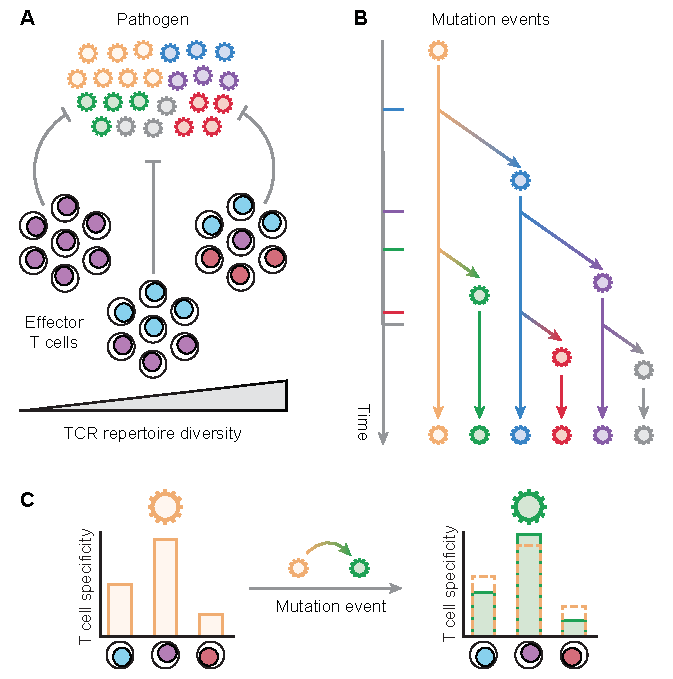
\includegraphics[width=0.64\textwidth]{Figures/VE/fig1_scheme.pdf}
    \caption[Computational population model of effector T cell diversity in response to a mutating pathogen]{\textit{Computational population model of effector T cell diversity in response to a mutating pathogen}. %
    %
    \secbfcolor{(A)}~Schematic illustrating effector T cells of varying TCR repertoire diversity responding to different variants of a replicating pathogen. %
    %
    \secbfcolor{(B)}~The pathogen is allowed to mutate within the model; the likelihood of a mutation event is proportional to the abundance of the parent strain. %
    %
    \secbfcolor{(C)}~Each T cell clone is assigned a value equivalent to the specificity of that clone for a pathogen strain. Upon mutation, the specificity of a T cell clone for a mutant strain is perturbed relative to its specificity for the parent strain.}
    \label{fig:VE_scheme}
\end{figure}
%
In the model, pathogen strains can give rise to mutant daughter strains throughout the infection (Fig.~\ref{fig:VE_scheme}B), with a mutation rate that is proportional to the abundance of the parental strain (i.e., strains with high pathogen loads are more likely to generate mutant progeny than ones with lower pathogen loads). To every pair of T cell clones and pathogen strains, we assign a value representing the specificity of that clone for that strain of the pathogen. Upon mutation, the specificity of any T cell clone for the daughter strain is assumed to be a small deviation in magnitude from its specificity for the parental strain (Fig.~\ref{fig:VE_scheme}C).

By simulating the model with one initial strain of the pathogen and $N=100$ unique TCR clonotypes, we generated time series showing different strains of the pathogen emerging in succession (Fig.~\ref{fig:VE_timeSeries}A) and the resulting T cell response across all clonotypes (Fig.~\ref{fig:VE_timeSeries}B). When quantifying the number of clonotypes whose cell numbers represent 95\% of the total responding T cell count, a metric that we used to measure the diversity of the responding T cell population at any given point in time, we found that clonotype diversity contracts at later time points relative to peak infection (Fig.~\ref{fig:VE_timeSeries}C); this is consistent with previous observations in early vs. late stages of infection with LCMV-Cl13~\cite{chang2020t}. Of note, the imbalanced, upward-branching architecture of the phylodynamic tree constructed from these simulations confirmed that the pathogen is indeed evolving under selective pressure exerted by T cells~\cite{volz2013viral}. Given that the model was able to reproduce TCR clonotype dynamics in the context of chronic infection and pathogen evolution under T cell pressure, we could thus begin to probe how mutational burden (i.e., the number and abundance of emerging pathogen variants) is affected by this selective pressure.
%
\begin{figure}[t]
    \centering
    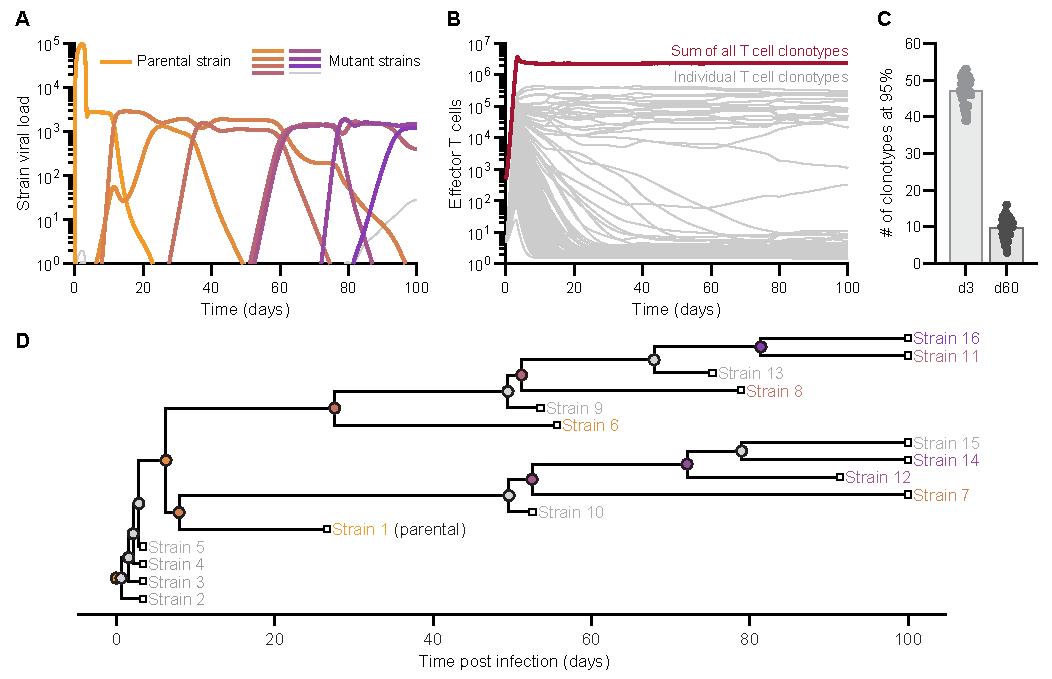
\includegraphics[width=\textwidth]{Figures/VE/fig2_timeSeries.pdf}
    \caption[Model simulations of the T cell response to mutating pathogen captures contraction of clonotype diversity over time]{\textit{Model simulations of the T cell response to mutating pathogen captures contraction of clonotype diversity over time}. %
    %
    \secbfcolor{(A)}~Pathogen load for each individual strain obtained from a single realization simulated by the model, starting from a single parental strain (Strain 1). Dominant strains (colored curves) are distinguished from those lowly abundant ones (gray curves) that make up $<$2\% of the pathogen pool at any given time. %
    %
    \secbfcolor{(B)}~Total number of effector T cells over time (red curve), comprised of 100 individual T cell clonotypes (gray curves) obtained from one single realization simulated by the model. %
    %
    \secbfcolor{(C)}~Number T cell clonotypes that make up 95\% of the responding T cell population at early vs. late stages of a chronic infection, computed from 50 independent realizations of model simulations. %
    %
    \secbfcolor{(D)}~Phylodynamic tree showing pathogen evolution over time. Strains are numbered according to their order of appearance and color-coded according to the traces shown in A. %
    }
    \label{fig:VE_timeSeries}
\end{figure}


\subsection{The number of dominant mutants is distinct from the total mutation rate}

Previous work has shown that the frequency of LCMV-Cl13 viral mutants 39 to 75 days post-infection in RAG2\KO{} mice (lacking both functional T and B cells) are negligible when compared to those in WT mice~\cite{smyth2021characterization}. Having developed our model of pathogen evolution, we asked whether the model produces similar results when simulated in the presence or absence of the effector T cell pool. To test this, we first simulated 200 independent realizations of the model in the absence of T cells or with $N=100$ unique T cell clonotypes, starting with a single parental strain, and quantified the cumulative number of strains of the pathogen that emerges over the course of each simulation (Fig.~\ref{fig:VE_noTcells}A,~B). Seemingly in contrast to the data from LCMV-Cl13 infections in RAG2\KO{} mice, we observed a greater absolute number of mutants over the course of an infection in the absence of T cells in the model (Fig.~\ref{fig:VE_noTcells}B). In fact, the number of total strains mirrored the simulated pathogen loads, with higher levels of pathogen obtained in the absence than in the presence of T cells  (Fig.~\ref{fig:VE_supp_noTcells}A). We experimentally verified this result by quantifying LCMV-Cl13 viral titres in WT and TCR\textbeta{}\KO{} mice 14 days post-infection, finding that indeed TCR\textbeta{}\KO{} mice possessed higher LCMV-Cl13 glycoprotein (GP) RNA levels relative to WT mice (Fig.~\ref{fig:VE_supp_noTcells}B,~C). This direct relationship between pathogen load and the total strain count in the model was not surprising, given that the rate of mutation was assumed to scale linearly with pathogen abundance in the model.
%
\begin{figure}[t]
    \centering
    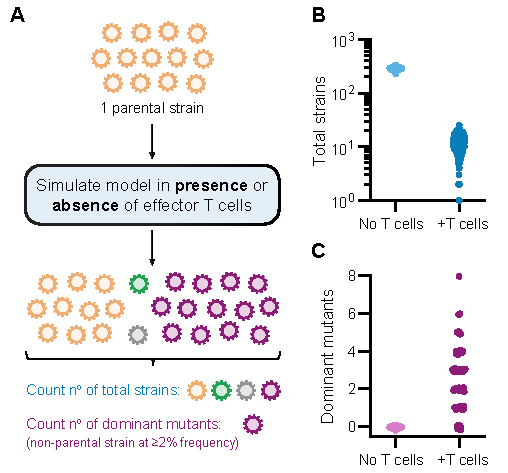
\includegraphics[width=0.48\textwidth]{Figures/VE/fig3_noTcells.pdf}
    \caption[Absence of selective pressure by T cells results in lack of dominant mutants despite high mutation rates]{\textit{Absence of selective pressure by T cells results in lack of dominant mutants despite high mutation rates}. %
    %
    \secbfcolor{(A)}~A schematic illustrating how model simulations are performed in the presence and absence of effector T cells, starting with a single parental strain. The total (i.e. cumulative) number of strains and the number of dominant mutants (non-parental strains present at a frequency of at least 2\% at any point of the simulation) appearing throughout the simulation are quantified. %
    %
    \secbfcolor{(B,C)}~Total number of strains (B) and number of dominant mutants (C) arising by 100 days post-infection predicted by the model, in the absence of T cells or when the number of T cell clones $N$ is set to 100. Data shown result from 200 independent realizations of model simulations.%
    }
    \label{fig:VE_noTcells}
\end{figure}
%

In light of the apparent discrepancy regarding mutational burden between our model and data from RAG2\KO{} mice, we reasoned that a more biologically relevant metric would not be the total number of mutants, but rather those that are sufficiently abundant (or ``dominant") relative to the overall pathogen load since these mutants would presumably have a greater impact on the infected host and on disease transmission at the epidemiological scale. Furthermore, it is worth noting that variants present at low relative abundances cannot be reliably detected using conventional sequencing techniques. Indeed, it has been estimated that variants present at a frequency below $\sim$2\% cannot be confidently identified~\cite{lauring2020within}, although this threshold value for variant identification is not fixed but rather strongly dependent on the input genome size~\cite{mccrone2016measurements}, among other factors. Based on this argument, we decided to instead quantify the number of ``dominant'' mutants, defined as the variants of the parental strain that each constitute a minimum of 2\% of the total pathogen load at any given time throughout the simulation. Indeed, when we quantified the number of dominant mutants predicted by the model with or without effector T cell control, we found no dominant mutants arise in the absence of T cells, despite a larger number of total strains (Fig.~\ref{fig:VE_noTcells}A,~C). This finding thus agrees with previous data showing a lack of measured mutational burden in the absence of selective pressure from adaptive immunity~\cite{smyth2021characterization}, and highlights the importance of distinguishing dominant mutants from other, more lowly abundant variants in subsequent model analyses.

\subsection{Intermediate TCR repertoire diversity can lead to higher numbers of dominant mutants that evade the T cell response \textit{in silico}}

\begin{figure}[b!]
    \centering
    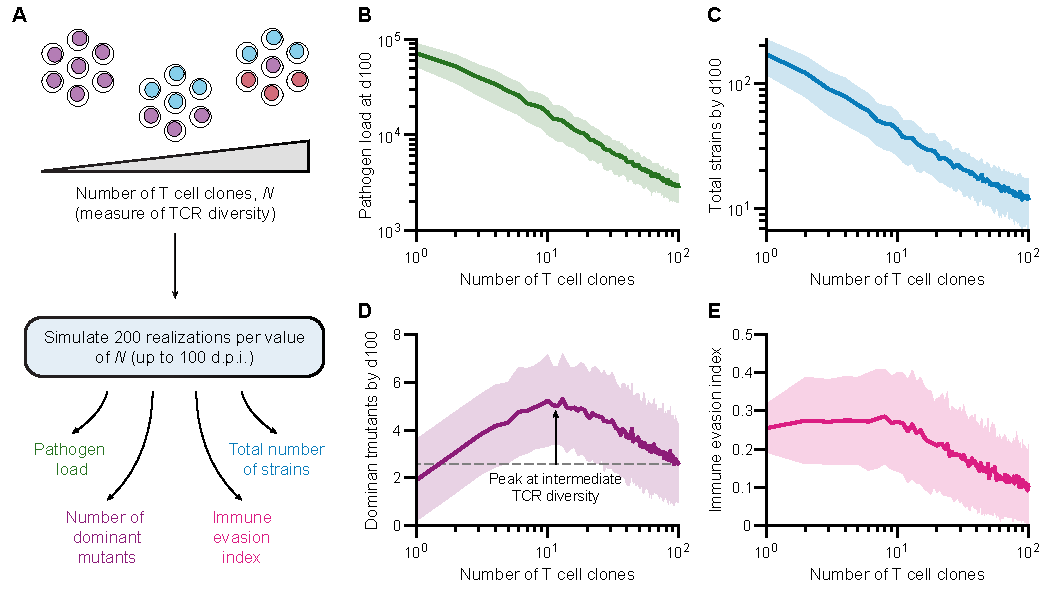
\includegraphics[width=\textwidth]{Figures/VE/fig4_effectOfN.pdf}
    \caption[Intermediate level of TCR repertoire diversity in the model promotes greater levels of immune escape]{\textit{Intermediate level of TCR repertoire diversity in the model promotes greater levels of immune escape}. %
    %
    \secbfcolor{(A)}~A schematic illustrating how model simulations are performed when the number of effector T cell clones, a parameter representing TCR diversity in the model, is gradually varied to test its effect on pathogen replication and evolution over time. %
    %
    \secbfcolor{(B,~C)}~Simulations of pathogen load by day 100 post-infection~(B) and total number of pathogen strains that emerges over the course 100 days~(C) as a function of the number of T cell clones considered in the model. %
    %
    \secbfcolor{(D,~E)}~Number of dominant mutants (D), defined as the number of strains other than the starting strain with $\geq$2\% abundance at any point in time, and pathogen evasion index (E), representing the degree with which escape mutants evade T cell recognition, as a function of the number of T cell clones. Dashed line in D indicates the average number of dominant mutants for $N=100$. Curves in panels B-E represent the mean over 200 realizations of model simulations, and shaded areas represent $\pm$ standard deviation. %
    }
    \label{fig:VE_effectOfN}
\end{figure}
Having verified model outcomes at the two ends of the T cell diversity spectrum (i.e., when there are no T cells or there are many unique T cell clones), we next asked how gradually varying the number of T cell clonotypes impacts pathogen evolution across this spectrum  (Fig.~\ref{fig:VE_effectOfN}A). In doing so, we found that the total pathogen load and, consequently, the total number of strains that emerge over the course of the simulated 100-day period were inversely proportional to the number of T cell clones in the model (Fig.~\ref{fig:VE_effectOfN}B,~C), suggesting that more diverse TCR repertoires provide increased control of pathogen replication overall. Interestingly, however, when we quantified the number of dominant mutants as a function of TCR diversity, we found that more mutants emerge on average at intermediate levels of TCR diversity (Fig.~\ref{fig:VE_effectOfN}C).

Since we were interested in pathogen immune escape as a function of TCR diversity, we wondered whether responding T cells in the model were less specific overall for the mutants that do become dominant relative to the parental strain at intermediate TCR diversity values. To investigate this, we developed a metric that we termed the ``immune evasion index'', which measures the degree with which dominant mutants evade recognition by T cells in the model (see Methods). When calculating the value of this index as a function of TCR diversity, we indeed found that intermediate values of repertoire diversity not only promotes the formation of more dominant mutants (Fig.~\ref{fig:VE_effectOfN}D), but that these mutants are less recognizable by responding T cells than dominant mutants emerging at higher TCR diversity (Fig.~\ref{fig:VE_effectOfN}E). Importantly, however, this observation is dependent on model parameters; for example, gradually increasing \textit{inter}-clonal competition to be identical to \textit{intra}-clonal competition among responding T cells abolishes this effect and the number of dominant mutants instead approaches a plateau as TCR diversity is increased (Fig.~\ref{fig:VE_supp_asymComp}). Nonetheless, these data suggest that insufficient TCR repertoire diversification might lead to more immune escape in certain parameter regimes, and that this observation has potential implications in the case of T cells lacking TdT-dependent N-nucleotide diversification.


\subsection{Optimal range of pathogen loads promote highest levels of mutational burden}

\begin{figure}[b!]
    \centering
    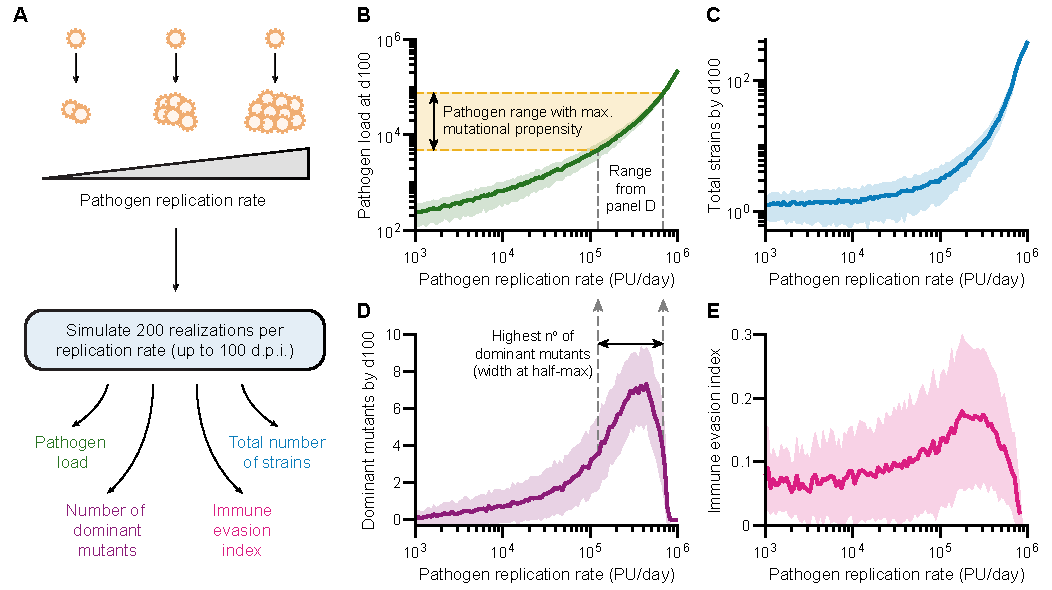
\includegraphics[width=\textwidth]{Figures/VE/fig5_effectOfBeta.pdf}
    \caption[High mutational burden and more immune escape occur within an optimal range of pathogen loads]{\textit{High mutational burden and more immune escape occur within an optimal range of pathogen loads}. %
    %
    \secbfcolor{(A)}~A schematic illustrating how model simulations are performed to investigate the effect of equilibrium pathogen loads on its evolution; the pathogen replication rate (parameter $r_P$ in the model, see Methods) is gradually increased and model outcomes are assessed as in Fig.~\ref{fig:VE_effectOfN}. The number of T cell clones, $N$, is held constant at a value of 50 clones. %
    %
    \secbfcolor{(B,~C)}~Simulations of pathogen load by day 100 post-infection~(B) and total number of pathogen strains that emerges over the course 100 days~(C) as a function of the rate of pathogen replication.
    %
    \secbfcolor{(D,~E)}~Number of dominant mutants (D), and pathogen evasion index (E), as a function of pathogen replication rate. The half-maximum width of the curve in D is used to determine the range of pathogen loads in B that maximally promote the emergence of dominant mutants (yellow-shaded region). Curves represent the mean over 200 realizations of model simulations, and shaded areas represent $\pm$ standard deviation.}
    \label{fig:VE_effectOfBeta}
\end{figure}

In light of our observations thus far, we wished to further investigate the reason for the divergent relationship between \textit{dominant} mutant emergence as compared to pathogen load and the \textit{total} number of mutants. Based on previous modelling work~\cite{grenfell2004unifying}, we hypothesized that there exists an optimal zone of pathogen load where the amount of replicating pathogen is high enough to maintain a high mutation rate, but also low enough that new, more evasive mutants can readily overtake the strains that are dominant upon its emergence. To directly test this, we checked whether we would observe similar results by gradually increasing equilibrium pathogen loads in the model, while keeping all other parameters constant. Since we do not have an explicit parameter representing pathogen load, this was achieved by varying the pathogen replication rate parameter ($r_P$, see Methods) (Fig.~\ref{fig:VE_effectOfBeta}A). Our results showed that, whereas pathogen loads and the total number of strains increase monotonically with increasing pathogen replication rates (Fig.~\ref{fig:VE_effectOfBeta}B,~C), the number of dominant mutants peaks before falling off sharply when both pathogen replication and loads are high (Fig.~\ref{fig:VE_effectOfBeta}D,~B). We observed a similar trend when we additionally quantified the immune evasion index (Fig.~\ref{fig:VE_effectOfBeta}E), which mirrors the number of dominant mutants by peaking at intermediate pathogen replication rates.

While the above model outcomes were measured as a function of pathogen replication rate, in this analysis, we used this parameter specifically to modulate pathogen load (Fig.~\ref{fig:VE_effectOfBeta}B). In order to relate these observations made with respect to pathogen replication rates back to pathogen loads, we determined what equivalent range of the latter promotes the highest levels of dominant mutants; to do this, we computed the width at half-maximum of the curve in Fig.~\ref{fig:VE_effectOfBeta}D, and determined the corresponding range of pathogen loads by relating it back to the curve in Fig.~\ref{fig:VE_effectOfBeta}B. We define this range of pathogen loads, resulting in more than half of the average maximum number of dominant mutants, as having maximal ``mutational propensity'' (Fig.~\ref{fig:VE_effectOfBeta}B). This range exists due to competition for replication between different strains of the model, which is a feature of the model that ensures accurate behaviour when multiple strains are present (see Section~\ref{sec:VE_modelDesign} -- Model design); briefly, when pathogen loads are high, competition for replication within target cells makes it less likely for newly emerged, lowly abundant mutants to overtake the existing pool of strains despite high mutation rates. In summary, the model suggests that an intermediate range of pathogen loads exists that maximally promotes the emergence of escape mutants, and that this results from a balance between sufficient rates of mutation and competitive dynamics among strains.

\subsection{The rate of immune escape depends on a balance between pathogen intrinsic and T cell-dependent mechanisms}

Our previous result suggests that changes in pathogen dynamics can alter the number of dominant mutants that emerge, with an optimal range of pathogen loads displaying maximal mutational propensity. However, we wondered whether we could tease apart the contributions to immune escape of the intrinsic properties of the pathogen vs. those that depend on T cell control, and how these processes interact to generate the model outcomes observed thus far. To investigate this, we gradually varied the number of T cell clones, and for each individual diversity value, we repeated the analysis described in the previous section to measure how maximal mutational propensity changes as a function of TCR diversity (Fig.~\ref{fig:VE_supp_maxMutProp}A). Interestingly, we found that more dominant mutants can emerge at higher numbers of T cell clones within the range of maximal mutational propensity (Fig.~\ref{fig:VE_supp_maxMutProp}B), indicating greater selection pressure exerted by T cells on pathogen evolution with increasing TCR diversity.

\begin{figure}[t!]
    \centering
    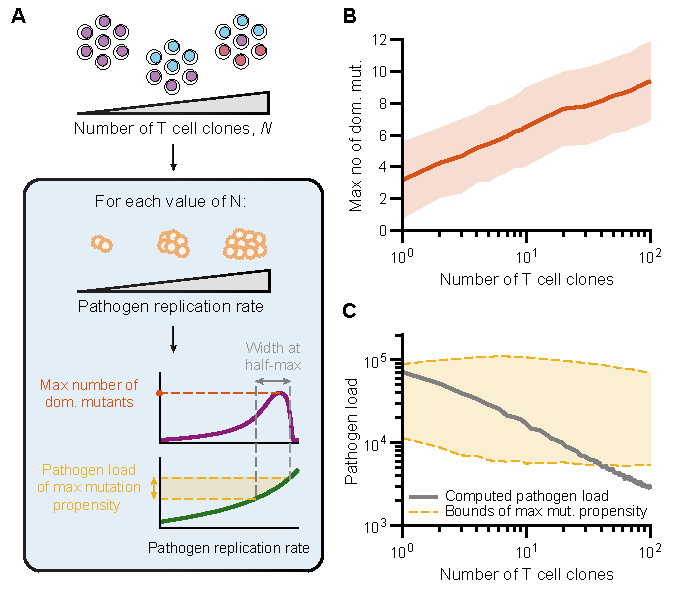
\includegraphics[width=0.64\textwidth]{Figures/VE/fig6_maxMutProp.pdf}
    \caption[Peak in number of dominant mutants at intermediate TCR diversities can be explained by the balance between pathogen control and T cell selective pressure]{\textit{Peak in number of dominant mutants at intermediate TCR diversities can be explained by the balance between pathogen control and T cell selective pressure}. %
    %
    \secbfcolor{(A)}~A schematic illustrating how model simulations are performed by gradually varying the number of T cell clones, $N$, and at each value of $N$ the relationship between pathogen replication rate and the number of dominant mutants is computed as described previously (Fig.~\ref{fig:VE_effectOfBeta}); the goal is to determine the maximum number of dominant mutants, and the range of pathogen loads with the highest mutational propensity, as a function of $N$. %
    %
    \secbfcolor{(B)}~The maximum expected number of dominant mutants is higher for higher TCR diversity, indicating that T cell control exerts more selective pressure on pathogens. Curve: mean, shaded region: standard deviation. %
    %
    \secbfcolor{(C)}~Despite higher selective pressure for large numbers of T cell clones, greater pathogen control decreases computed pathogen abundances (gray curve, identical to Fig.~\ref{fig:VE_effectOfN}B) below the range of pathogen loads with the highest mutational propensity (shaded region bounded by dashed lines).} 
    \label{fig:VE_supp_maxMutProp}
\end{figure}

However, while greater TCR diversity leads to more selection pressure on the evolving pathogen, we previously showed that increasing the number of T cell clones also reduces the total pathogen load (Fig.~\ref{fig:VE_effectOfN}B), and that the number of dominant mutants peaks at intermediate TCR diversities before coming back down when the number of unique clones is higher (Fig.~\ref{fig:VE_effectOfN}D). Thus, we wondered whether we could reconcile these findings by comparing the total pathogen load predicted by the model against the range of pathogen loads with maximal mutational propensity, both as a function of TCR diversity. Indeed, by overlaying the observed pathogen load (computed as shown previously in Fig.~\ref{fig:VE_effectOfN}B) onto the computed range within which higher numbers of dominant mutants arise (Fig.~\ref{fig:VE_supp_maxMutProp}C), we found that increasing the number of T cell clones drives pathogen loads below this range, thus explaining why fewer dominant mutants are observed than would be expected based purely on selection pressure alone. Of note, we observed that the range of pathogen loads with maximal mutational propensity is relatively independent of TCR diversity, suggesting that this range is intrinsic to pathogen replication dynamics. Taken together, these data suggest that while the optimal range of pathogen loads favouring the emergence of evasive dominant mutants is largely dependent on the intrinsic properties of the pathogen, different levels of T cell control can alter pathogen loads, and thus mutational burden, relative to this range. Hence, the peak in the rate of immune escape at intermediate TCR diversities can be explained by a balance between higher selective pressure on pathogen strains and insufficient control of pathogen replication.


\section{Discussion}

Despite the important role that T cell activity plays in shaping pathogen evolutionary landscapes, there has been surprisingly limited work aimed specifically at addressing how TCR diversity interacts with pathogen intrinsic dynamics to promote immune escape. Our modelling results propose that when the amount of pathogen falls within a specific range, its propensity for generating mutants that can then efficiently replicate within the host is maximized. We found that, while this range is largely independent of T cell control, it dictates how T cell diversity can influence pathogen evolution by modulating pathogen loads relative to this range. More specifically, our results revealed that while more T cell control can lead to higher evolutionary selection pressure on the mutating pathogen (driving the potential number of escape variants up), but it also lowers total pathogen loads, bringing the latter outside the intrinsic range of maximal mutational propensity and causing the number of escape variants to go down. In other words, the resulting mutational burden of the pathogen on the host will depend on the balance between these two opposing forces. We showed that a potential consequence of these interacting dynamics is a peak in the rate of immune escape at intermediate values of TCR diversity, with otherwise fewer dominant mutants being observed on average when the number of responding T cell clonotypes is comparatively lower or higher.

Importantly, our findings could have implications with regard to TCR repertoire diversification via TdT. While TdT-deficient hosts, with about 10-fold fewer unique T cell clonotypes~\cite{davis1988t,murugan2012statistical,zarnitsyna2013estimating}, were hypothesized to be more prone to immune escape by pathogens relative to their WT counterparts owing to the presence of repertoire ``holes''~\cite{vrisekoop2014revisiting}, no subsequent work has directly tested this hypothesis. Our model suggests that it is certainly plausible for higher rates of immune escape (in the form of dominant mutants) %with higher immune evasion indices in the model
to result from a 10-fold reduction in TCR repertoire diversity relative to baseline (Fig.~\ref{fig:VE_effectOfN}), provided that an increase in TCR diversity is accompanied by greater control of pathogen replication (and hence lower pathogen loads). We also know from our previous work that mice chronically infected with LCMV-Cl13 have higher viral loads than WT mice when TdT is lacking in their T cells~\cite{jamaleddine2022chronic}. One can thus infer, based on our model predictions, that LCMV-Cl13 viral loads might fall within the range of maximal mutational propensity that favours the production of escape variants in the absence of TdT. Using existing sequencing tools that can assess within-host pathogen diversity~\cite{lauring2020within}, subsequent experimentation will be able to test our model prediction to determine whether another evolutionary advantage of TdT is indeed to protect hosts from mutating pathogens.

Interestingly, it is known that T cells lacking N-nucleotide diversity from TdT are more cross-reactive than those with N-diversity, which was proposed as an explanation for the lack of TdT expression in neonates~\cite{gavin1995increased}. It should be noted that our model does not consider differences in cross-reactivity for less diverse TCR-repertoire or how this could impact the emergence of escape variants, though presumably incorporating such a mechanism might partially compensate for the lower number of unique clones and diminish the peak in the number of dominant mutants at intermediate diversity. We also showed that this effect was dependent on certain parameters of the model (including the ratio between inter- and intra-clonal competition), and that there exist regimes in parameter space where intermediate TCR diversities do not generate higher numbers of unique clones (Fig.~\ref{fig:VE_supp_asymComp}). It is thus important to note that the model does not definitively conclude that TdT-deficient TCR repertoires are more susceptible to immune escape by mutating pathogens, but rather suggests that these dynamics are theoretically possible and that this merits further investigation to confirm whether or not TdT benefits host immune responses by limiting escape.

While our model was kept simple in order to focus on the effects of T cell clonal diversity on pathogen immune escape, other elements that were not included explicitly also exert their effects on the evolutionary dynamics of pathogens that are worth noting. For example, our model assumes that pathogen replication rate is unchanged upon mutation, and that there is an equal chance for T cell specificity for the mutant strain to be higher or lower than that of the parent strain. However, it has been established in the context of viral quasispecies evolution that a large number of mutations are deleterious or even lethal for pathogens, and that overall fitness tends to decrease across generations~\cite{bergstrom1999transmission,peck2018complexities,wylie2011biophysical}. Thus, while incorporating the effect of more realistic fitness landscapes would increase the complexity of the model, it certainly remains of relevance to ask how such inclusions could affect predicted outcomes and how TCR diversity profiles impact pathogen evolution across realistic fitness valleys.

Our finding that the range of pathogen loads with maximal mutational propensity is largely invariant to different levels of T cell selective pressure was quite intriguing to us. Incidentally, earlier theoretical work on viral-immune co-evolution analogously showed that an optimal mutation rate exists that maximizes immune escape, and that the experimentally calculated per-genome average mutation rate of HIV-1 lies near this optimum~\cite{kamp2002viral}. It is thus conceivable that this notion extend to pathogen loads as suggested by our model, since the abundance of replicating pathogen will itself dictate the total number of mutations for a given mutation rate. Strikingly, however, while the mutation rate per base pair varies by orders of magnitude across different types of DNA and RNA viruses, when accounting for the entire genome size, the per-genome average mutation rate is relatively similar across different species of viruses~\cite{sanjuan2016mechanisms,peck2018complexities}. In spite of this, within-host viral phylogenies still vary substantially~\cite{grenfell2004unifying}. While this undoubtedly depends on many interconnected aspects of the pathogen biology and the resulting immune response, perhaps viral set points in HIV and HCV, which produce chronic infections in hosts and show substantial evidence of evolution in response to immune pressure~\cite{grenfell2004unifying, raghwani2019high,lemey2006hiv}, fall within these ranges of maximum mutational propensity so as to optimally adapt to the host immune landscape. 

In summary, by applying the principles of pathogen-immune co-evolution to specifically study the impact of TCR diversity on immune escape, interesting predictions arose from model results that are worth further experimental investigation. In addition, our observations led to intriguing insights that may extend beyond the scope of TCR diversity, having potentially broader implications to pathogen evolution more generally.

\section{Methods}

\subsection{Mice}

C57BL/6  and TCR\textbeta{}\KO{} mice~\cite{mombaerts1992mutations} were purchased from Jackson Laboratories (Bar Harbor, ME). % \red{The TdT\KO{} mice were shared by Dr. A. Feeney (The Scripps Research Institute)~\cite{gilfillan1993mice}}.
All mice were on a C57BL/6 background, bred in-house and experiments performed at 8-13 weeks of age with only males. Animal housing, care, and research were in accordance with the Guide for the Care and Use of Laboratory Animals and all procedures performed were approved by the McGill University Animal Care Committee.

\subsection{LCMV-Cl13 stock and infections}

The Clone 13 strain of LCMV was propagated from stocks provided by Dr. M. Richer (University of Indiana) on L929 cells, as described previously~\cite{jamaleddine2022chronic}. Mice were infected by injecting 2\E{6} plaque forming units (PFU) of LCMV-Cl13 intravenously as per established protocol~\cite{wherry2003viral,richer2013pathogen}. Mice were sacrificed 14 days post-infection, and their spleens were collected in 1\%~RPMI before being weighed and homogenized in Lysing Matrix D tubes (MP Biomedicals) using a MagNA Lyser (Roche) at 6000~rpm for 40~seconds. Spleen homogenate was then spun down at 12,000~rpm for 10 minutes at 4\degree{C}. To further clarify the solution, the supernatant was transferred to a new sterile tube and re-spun at 12,000 rpm for 10 minutes at 4\degree{C}, and 400~\textmu{}L of TRIzol reagent (Invitrogen) was added to 200~\textmu{}L aliquots of the supernatant from homogenized spleens before being stored at $-80$\degree{C} for RNA processing and quantification of viral titres.

\subsection{RNA extraction and viral titre determination}

To quantify viral loads in the spleens of WT or TCR\textbeta{}\KO{} mice, samples were thawed on ice before adding 80~\textmu{}L of chloroform, incubating at room temperature for 5 minutes, and spinning down at 12,000~rpm for 15 minutes. RNA was extracted using the PureLink RNA Mini Kit (Invitrogen), followed by cDNA conversion of 220~ng of RNA in 20~\textmu{}L reaction volumes with the High-Capacity cDNA Reverse Transcription Kit (Invitrogen). Viral titres were determined via qPCR to quantify LCMV-GP RNA levels using primers described previously~\cite{welsh2008lymphocytic}.

\subsection{Statistical analyses of experimental data}

Group comparisons were performed using MATLAB version 2022a. Information about implemented statistical tests and sample sizes for individual experiments is provided in the figure legends.

\subsection{Computational model}

\subsubsection*{Model formalism}
To model the dynamics of pathogen evolution as a function of TCR repertoire diversity, we constructed an ordinary differential equation (ODE) model consisting of $N$ fixed clones of effector T cells $E_i(t)$ ($i \in \{1,\,2,\,...,\,N\}$) and $M(t)$ strains of a mutating pathogen $P_j(t)$ ($j \in \{1,\,2,\,...,\,M(t)\}$), where the total number of pathogen strains, $M(t)$, is allowed to increase with time via random mutation events. The system of equations describing the model can be written as
%
\begin{align}
    \dv{E_i}{t} &= \frac{\sigma_E}{N} + r_E E_i \sum_{j=1}^{M(t)}\left(\frac{P_j}{P_\textup{tot} + k_{ij}} \right) -\delta_E E_i - \varepsilon E_i \sum_{n=1}^N \omega_{in} E_n, \label{eq:VE_E} \\[0.5em]
    \dv{P_j}{t} &= r_P \frac{P_j}{P_{\textup{tot}}+P_h} - \delta_P P_j - \kappa_P \sum_{i=1}^{N}\left(E_i \frac{P_j}{P_{\textup{tot}} + k_{ij}} \right). \label{eq:VE_P}
\end{align}

Equation~\eqref{eq:VE_E}, describing the rate of change of effector T cell clone $i$ over time, was adapted from previous models of T cell dynamics~\cite{jamaleddine2020quantifying,jamaleddine2022chronic,khadra2011investigating,jaberi2015continuum}. The source term $\sigma_E$ represents total thymic input of all pathogen-specific T cells; although different clonotypes are present at different precursor frequencies in the na\"{i}ve T cell repertoire~\cite{quigley2010convergent}, for simplicity we let thymic input be equally divided among all $N$ T cell clones. All clones are assumed to share a natural turnover rate given by $\delta_E$, and to proliferate with a maximum rate $r_E$ upon pathogen recognition. The contribution of each strain of pathogen, $P_j$, will depend on the abundance of that strain relative to the total pathogen load, denoted by $P_{\textrm{tot}} = \sum_j P_j$, and on the specificity of T cell clone $i$ for strain $j$, a value that depends reciprocally on the magnitude of the parameter $k_{ij}$. This latter parameter is sampled randomly from a log-normal distribution, with base-10 logarithmic mean $\mu_k$ and standard deviation $\sigma_k$. The final term in Eq.~\eqref{eq:VE_E} represents the rate of intra- and inter-clonal competition among T cells. We let the rate of intra-clonal competition be equal to $\varepsilon$, which represents competition for cognate antigen as well as other survival signals~\cite{khadra2009role,jamaleddine2020quantifying,jamaleddine2022chronic}, and let inter-clonal competition occur at a lower rate $f \times \varepsilon$, where $f<1$ (since different T cell clones may have different antigen specificity). In other words, we assumed that
%
\begin{equation*}
    \omega_{in} = 
    \begin{cases}
        1 \qquad \textrm{if} \qquad i=n, \\
        f \qquad \textrm{otherwise}.
    \end{cases}
\end{equation*}

The rate of change of each pathogen strain $P_j$ as a function of time is described by Eq.~\eqref{eq:VE_P}. We assumed that the \textit{per capita} replication rate of each strain is upper-bounded by the fraction $r_P/P_h$, and that, when pathogen loads are sufficiently high (i.e., when $P_{\textrm{tot}} > P_h$), more abundant strains have a higher probability of invading target cells and thus replicate more efficiently. We let $\delta_P$ be the rate that encompasses all T cell independent mechanisms of pathogen clearance, while the final term in Eq.~\eqref{eq:VE_P} represents T cell-mediated pathogen clearance of strain $j$ at a maximum rate of $\kappa_P$ per T cell clone $i$. We assumed this rate to be dependent again on the specificity of clone $i$ for strain $j$, represented by the reciprocal of $k_{ij}$, as well as the relative abundance of strain $j$.

\subsubsection*{Mutation events}

Generation of mutant strains in the model was obtained using a non-homogeneous Poisson point process, where the stochastic frequency of novel variant formation from a parental strain was assumed to be proportional to the abundance of that strain, modulated by an average \textit{per capita} mutation rate. To do this, at each time step $\Delta t$ in the simulation, we sampled a number $M_{\textup{new}}$ arising from strain $P_j$ from a Poisson distribution with rate parameter $\lambda (t) = r_{\textup{mut}} \, P_j(t) \, \Delta t$, similar to previous modelling work on HIV evolution~\cite{nowak1991antigenic}. To prevent long computational times, we did not allow new variants to be produced once the total number of strains exceeded a high number $M_{\textup{max}}$.

When a new variant, $P_m$, is formed from $P_j$, we assumed that the specificity of each T cell clone $i$ for the new strain $m$ is perturbed relative to that of clone $i$ for the parental strain $j$. To implement this, we let the magnitude of the perturbation be drawn from a log-normal distribution, with a standard deviation $\theta_k$ and centered at 0 in base-10 logarithmic space, i.e., $\log_{10}(k_{im}) = \log_{10}(k_{ij}) + \mathcal{N}(0,\theta_k)$. This is illustrated schematically in Fig.~\ref{fig:VE_scheme}C, where the specificity of each clone $i$ for a given strain was assessed via the reciprocal of the parameter $k_{ij}$ or $k_{im}$ (for the parental strain $j$ or the mutant strain $m$, respectively).


\subsection{Model parameters and numerical implementation}

Table~\ref{tab:VE_parameters} summarizes the different parameters of the model and their respective values used in the simulations. These parameters and their values are similar to our previous work analyzing the dynamics of effector T cells responding to replicating pathogen~\cite{jamaleddine2022chronic} using a computational model that was fit to serum viral load data from LCMV-Cl13 infected mice~\cite{wherry2003viral}.

\begin{table}[ht]
\footnotesize
\centering
\begin{tabular}{p{0.06\textwidth} p{0.53\textwidth} p{0.12\textwidth} p{0.17\textwidth}}
    \hline
    \textbf{Param.} & \textbf{Description}                                             & \textbf{Value(s)} & \textbf{Units} \\
    \hline
    %
    $\sigma_E$ & Thymic input across all TCR clonotypes & 150 & cells~day$^{-1}$ \\
    %
    $r_E$ & Maximum proliferation rate of effector T cells & 4.0 & day$^{-1}$ \\
    $k_{ij}$ & Pathogen load of strain $j$ evoking half-maximum response of T cell clone $i$, drawn from a log-normal distribution &  Range & PU$^{-1}$ \\
    $\mu_k$ & Base-10 logarithmic mean used to sample $k_{ij}$ & 4.4 & --
    \\
    $\sigma_k$ & Base-10 logarithmic standard deviation used to sample $k_{ij}$ & 0.5 & -- \\
    %
    $\delta_E$ & Natural turnover rate of effector T cells & 0.3 & day$^{-1}$ \\
    %
    $\varepsilon$ & Intra-clonal competition rate & 3.2\E{-6} & cell$^{-1}$~day$^{-1}$ \\
    %
    $f$ & Scaling factor for inter-clonal competition & 0.1 & -- \\
    %
    $N$ & Number of unique pathogen-specific TCR clonotypes & Range & -- \\
    %
    $M_0$ & Initial number of pathogen strains & 1 & -- \\
    %
    $r_{P}$ & Maximum replication rate & 1.15\E{5} & PU~day$^{-1}$ \\
    %
    $P_h$ & Half-maximum constant of pathogen replication & 5\E{2} & PU \\
    %
    $\delta_P$ & T cell-independent pathogen clearance rate & 1 & PU~day$^{-1}$ \\
    %
    $\kappa_P$ & Maximum pathogen removal rate per T cell & 0.1 & PU~(cell~day)$^{-1}$ \\
    %
    $r_{\textup{mut}}$ & \textit{Per capita} average mutation rate used to randomly generate new pathogen strains & 2.5\E{-5} & day$^{-1}$ \\
    %
    $\theta_k$ & Base-10 logarithmic standard deviation used to sample perturbations of $k_{ij}$ from parent to daughter strain & 0.1 & --\\
    %
    $M_{\textup{max}}$ & Maximum allowable number of mutant strains per simulation & $10^4$ & -- \\
    \hline
\end{tabular}
\caption[Parameter values used in model simulations]{\textit{Parameter values used in model simulations}. These values were chosen to be similar to those in our previous modeling work of T cell control of replicating pathogen~\cite{jamaleddine2022chronic}. PU = pathogen units.}
\label{tab:VE_parameters}
\end{table}

In order to remove transient artifacts arising from improper initialization of the model, we first simulated the model in the absence of pathogen to allow the effector T cell population to reach a steady state; these steady state values were then used as the initial condition for effector T cells upon introduction of the parental strain of the pathogen in the model, where we set $P_1(t=0) \rightarrow 1$~PU (pathogen unit). Similarly, when a new strain $m$ is produced via a mutation event at time $t_m$, we set $P_m(t=t_m) \rightarrow 1$~PU. MATLAB version 2022a was used to write all codes and generate all numerical results pertaining to the model.

\section{Acknowledgements}

We would like to thank the animal facility staff at McGill University for their excellent care of our animal colony. H.J. was supported by an Alexander Graham Bell Canada Graduate Scholarship - Doctoral (NSERC) and a B2X Doctoral Award (FRQNT). J.N.M. is a Canada Research Chair for Immune Cell Dynamics. This work was supported by NSERC (Discovery Grant \#2019-04520 to A.K.) and a Mi4 seed grant (round 5, to J.N.M.).

\clearpage

\section{Supporting information}

\subsection{Supplemental figures}

\renewcommand{\thefigure}{S\thechapter.\arabic{figure}}
\renewcommand{\figurename}{Figure}
\setcounter{figure}{0}

\begin{figure}[h]
    \centering
    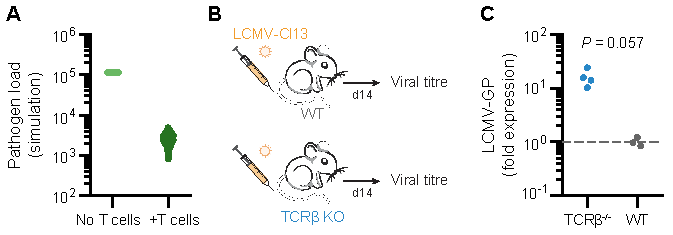
\includegraphics[width=0.64\textwidth]{Figures/VE/figS1_WTvsTCRb.pdf}
    \caption[Lack of host T cells leads to higher pathogen loads both \textit{in silico} and \textit{in vivo}]{\textit{Lack of host T cells leads to higher pathogen loads both \textup{in silico} and \textup{in vivo}}. %
    %
    \secbfcolor{(A)}~Pathogen loads at day 15 post-infection in the model when simulated in the absence or presence of effector T cells. %
    %
    \secbfcolor{(B)}~WT and TCR\textbeta{}\KO{} mice (n=3 and n=4, respectively) were infected with LCMV-Cl13, and spleens were harvested at day 14 for viral titre determination. %
    %
    \secbfcolor{(C)}~LCMV-GP RNA relative fold expression, assessed by qPCR. \textit{P}-value computed using non-parametric rank-sum test.}
    \label{fig:VE_supp_noTcells}
\end{figure}

\begin{figure}[h]
    \centering
    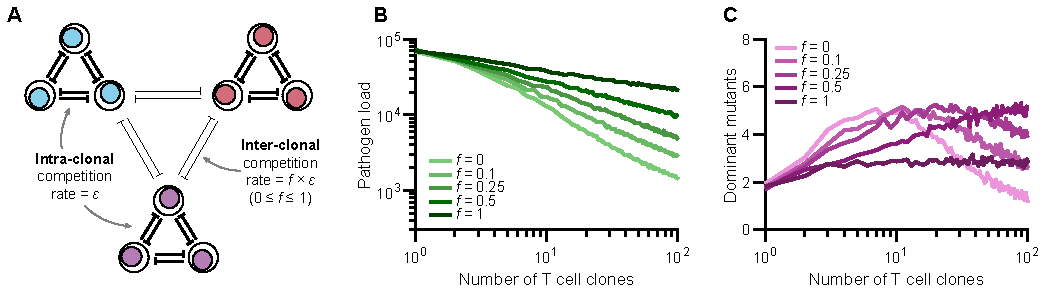
\includegraphics[width=\textwidth]{Figures/VE/figS2_asymComp.pdf}
    \caption[Symmetrical competition within and between T cell clones abolishes peak in mutational burden at intermediate TCR diversity]{\textit{Symmetrical competition within and between T cell clones abolishes peak in mutational burden at intermediate TCR diversity}. %
    %
    \secbfcolor{(A)}~Schematic depicting intra- vs. inter-clonal T cell competition. The inter-clonal competition is assumed to be a fraction, $0\leq f \leq 1$, of the inter-clonal competition rate $\varepsilon$. %
    %
    \secbfcolor{(B)}~Increasing $f$ from 0 (no inter-clonal competition) to 1 (symmetrical competition) reduces the effect of the number of clones $N$ on pathogen control.  %
    %
    \secbfcolor{(C)}~The number of dominant mutants does not peak as a function of TCR diversity when intra- and inter-clonal competition are similar, i.e., as $f\rightarrow1$.}
    \label{fig:VE_supp_asymComp}
\end{figure}

%%

\subsection{Model design}
\label{sec:VE_modelDesign}

The system of ODEs that describes the computational model in Eqs.~\eqref{eq:VE_E}-\eqref{eq:VE_P} were, in part, written as such in order to satisfy two important limits. The first limit considers the case where all effector T cell clones are identical and therefore have the same specificity for a given strain $j$. That is,
%
\begin{equation*}
   k_{1j} = k_{2j} = ... =  k_{Nj} \quad \equiv \quad k_{*j}.
\end{equation*}
%
In this case, the competition between these identical T cell clones would be fully symmetrical (since they would have the same antigen specificity), i.e., $\omega_{in} = 1, \; \forall \; i, n\in\{1,\dots,N\}$. Within this framework, the model should also be equivalent to a model with a single effector T cell clone ($N=1)$, denoted by $\tilde{E}$. To check this, we verified that the dynamics of the sum of identical clones, $E_{\textup{tot}} = \sum_i E_i$, are the same as those produced by $\tilde{E}$ whose specificity for strain $j$ is $1/k_{*j}$. The dynamics of this latter one-clone model are given by
%
\begin{align}
    \dv{\tilde{E}}{t} &= \sigma_E + r_E \tilde{E} \sum_{j=1}^{M(t)}\left(\frac{P_j}{P_\textup{tot} + k_{*j}} \right) -\delta_E \tilde{E} - \varepsilon \tilde{E}^2, \label{eq:VE_Etilde_E} \\[0.5em]
    \dv{P_j}{t} &= r_P \frac{P_j}{P_{\textup{tot}}+P_h} - \delta_P P_j - \kappa_P \tilde{E} \frac{P_j}{P_{\textup{tot}} + k_{*j}}. \label{eq:VE_Etilde_P}
\end{align}
%
By substituting $k_{ij} = k_{*j}$ and $\omega_{in} = 1$ in the original model of Eq.~\eqref{eq:VE_E} and writing it with respect to $\dv*{E_{\textup{tot}}}{t}$, we obtain
%
\begin{align*}
    \dv{E_{\textup{tot}}}{t} &= \sum_{i=1}^N \dv{E_i}{t} \\
    &= \sum_{i=1}^N \left( \frac{\sigma_E}{N} + r_E E_i \sum_{j=1}^{M(t)}\left(\frac{P_j}{P_\textup{tot} + k_{*j}} \right) -\delta_E E_i - \varepsilon E_i \sum_{n=1}^N E_n \right) \\[0.5em]
    &= \sigma_E + r_E E_{\textup{tot}} \sum_{j=1}^{M(t)}\left(\frac{P_j}{P_\textup{tot} + k_{*j}} \right) -\delta_E E_{\textup{tot}} - \varepsilon E_{\textup{tot}}^2,
\end{align*}
%
which, when setting $E_{\textup{tot}} = \tilde{E}$, matches exactly with Eq.~\eqref{eq:VE_Etilde_E}. Similarly, by applying these substitutions to Eq.~\eqref{eq:VE_P}, we obtain
%
\begin{align*}
    \dv{P_j}{t} &=r_P \frac{P_j}{P_{\textup{tot}}+P_h} - \delta_P P_j - \kappa_P \sum_{i=1}^{N}\left(E_i \frac{P_j}{P_{\textup{tot}} + k_{*j}} \right) \\[0.5em]
    &= r_P \frac{P_j}{P_{\textup{tot}}+P_h} - \delta_P P_j - \kappa_P E_{\textup{tot}} \frac{P_j}{P_{\textup{tot}} + k_{*j}}.
\end{align*}
%
This in turn matches exactly with Eq.~\eqref{eq:VE_Etilde_P} when setting $E_{\textup{tot}} = \tilde{E}$. It follows that when all effector T cell clones are identical, the two models are equivalent and the first limiting case is satisfied.

In the second limiting case, we apply a similar logic by making all pathogen strains to be identical, implying that any given T cell clone $i$ will be equally specific for all strains. By ignoring the time dependency of the maximum number of strains $M$ resulting from any new mutation event, we have
%
\begin{equation*}
   k_{i1} = k_{i2} = ... =  k_{iM} \equiv k_{i*}.
\end{equation*}
%
In this case, the model should be equivalent to a model with a single pathogen strain ($M=1)$, denoted by $\tilde{P}$. As before, we verified that the dynamics of the sum across all strains, $P_{\textup{tot}} = \sum_j P_j$, are the same as those produced by $\tilde{P}$, where the specificity of T cell clone $i$ for $\tilde{P}$ is equal to $1/k_{i*}$, by considering the one-strain model given by
%
\begin{align}
    \dv{E_i}{t} &= \frac{\sigma_E}{N} + r_E E_i \frac{\tilde{P}}{\tilde{P} + k_{i*}} -\delta_E E_i - \varepsilon E_i \sum_{n=1}^N \omega_{in} E_n, \label{eq:VE_Ptilde_E} \\[0.5em]
    \dv{\tilde{P}}{t} &= r_P \frac{\tilde{P}}{\tilde{P}+P_h} - \delta_P \tilde{P} - \kappa_P \sum_{i=1}^{N}\left(E_i \frac{\tilde{P}}{\tilde{P} + k_{i*}} \right). \label{eq:VE_Ptilde_P}
\end{align}
%
By substituting $k_{ij} = k_{i*}$ in Eq.~\eqref{eq:VE_E} of the original model and ignoring the time dependency of $M$,  we obtain
%
\begin{align*}
    \dv{E_i}{t} &= \frac{\sigma_E}{N} + r_E E_i \sum_{j=1}^{M}\left(\frac{P_j}{P_\textup{tot} + k_{i*}} \right) -\delta_E E_i - \varepsilon E_i \sum_{n=1}^N \omega_{in} E_n \\[0.5em]
    &= \frac{\sigma_E}{N} + r_E E_i \frac{P_\textup{tot}}{P_\textup{tot} + k_{i*}} -\delta_E E_i - \varepsilon E_i \sum_{n=1}^N \omega_{in} E_n,
\end{align*}
%
which, when setting $P_{\textup{tot}} = \tilde{P}$, matches exactly Eq.~\eqref{eq:VE_Ptilde_E}. Similarly applying these substitutions to Eq.~\eqref{eq:VE_P} and writing it with respect to $\dv*{P_{\textup{tot}}}{t}$, we obtain
%
\begin{align*}
    \dv{P_{\textup{tot}}}{t} &= \sum_{j=1}^{M} \dv{P_j}{t} \\[0.5 em]
    &= \sum_{j=1}^{M} \left( r_P \frac{P_j}{P_{\textup{tot}}+P_h} - \delta_P P_j - \kappa_P \sum_{i=1}^{N}\left(E_i \frac{P_j}{P_{\textup{tot}} + k_{i*}} \right) \right) \\[0.5em]
    &= r_P \frac{P_{\textup{tot}}}{P_{\textup{tot}}+P_h} - \delta_P P_{\textup{tot}} - \kappa_P \sum_{i=1}^{N}\left(E_i \frac{P_{\textup{tot}}}{P_{\textup{tot}} + k_{i*}} \right).
\end{align*}
%
This in turn matches exactly Eq.~\eqref{eq:VE_Ptilde_P} when setting $P_{\textup{tot}} = \tilde{P}$. This means that when all strains are identical, the two models are equivalent and the second limiting case is also satisfied.

Note that the second limiting case would not have been satisfied if $P_{\textup{tot}}$ in the denominator of the terms involved in effector T cell proliferation and T cell-dependent pathogen clearance (i.e., in $P_{\textup{tot}} + k_{ij}$), were replaced with $P_j$. In other words, if the proliferation of, and clearance by, T cells that are induced by a single pathogen strain were completely independent from the presence and abundance of other variants of that pathogen, then the model would depend arbitrarily on the number of strains despite all variants being physiologically indistinguishable. Similarly, if we had replaced $P_{\textup{tot}}$ in the denominator of the replication term of pathogen dynamics with $P_j$, the second limiting case would also no longer be satisfied.

By accounting for these limits when developing the model, we avoided generating results that were an artifact of its design. This form, however, introduces competition between different strains of the pathogen since, for example, the replication of a lowly abundant variant is disfavoured over a prominent one as a result of $P_{\textup{tot}}$ in the denominator of pathogen replication in Eq.~\eqref{eq:VE_P}; this in turn gives rise to an interesting result of the model, which is the pathogen intrinsic range of maximum mutational propensity (Figs.~\ref{fig:VE_effectOfBeta} and~\ref{fig:VE_supp_maxMutProp}). This is because, when the pathogen load of an abundant strain is too high, its competitive advantage makes it less likely for other variants to overtake it and thus for additional dominant mutants to arise. If, on the other hand, pathogen replication of a given strain were completely independent from the presence and abundance of other strains, we would expect the number of dominant mutants to more closely resemble the total number of strains arising from the simulations, i.e., we would no longer see a mismatch between these two metrics as we did in our model (Fig.~\ref{fig:VE_noTcells}). This reasoning provides support for our model prediction that T cell-dependent mechanisms contribute to, but cannot fully explain, immune escape, and that these work together with pathogen intrinsic properties to modulate the abundance and evasiveness of escape mutants.

\renewcommand{\thefigure}{\thechapter.\arabic{figure}}
\renewcommand{\figurename}{Figure}
\setcounter{figure}{0}

% \chapter{General discussion}
\label{sec:conclusion}

\section{Summary of research findings}

Despite the many advancements made to date in understanding how T cell antigen specificity and heterogeneity shape their dynamic anti-microbial or immunosuppressive responses, much remains that is yet to be uncovered. Across the three studies presented in this thesis, our primary aim was to use computational modelling to untangle some of these complexities, thus informing their resulting function in infection and autoimmunity and providing incremental advancements toward our general understanding of these phenomena.

First, in Chapter~\ref{sec:Tr1}, we sought to understand what biological factors could explain pMHC-NP treatment outcomes upon induction of autoimmune disorders in mice. We developed a compartmental population model to ask how Tr1 allocation and Tr1-mediated immunosuppression might together explain those experimental observations upon pMHC-NP administration. We found that Tr1 antigen specificity and binding avidity to APCs resulting from differences in cognate pMHC expression levels, together with recruitment kinetics into sites of autoimmune destruction, could account for differences observed in NP-therapy success vs. failure across experimental conditions.

Next, in Chapter~\ref{sec:AvC}, we were interested in adapting our model to study the effects of pMHC binding strengths in shaping T cell responses to acute or chronic pathogen replication. Together with experimental support, our model revealed differential evolution in pMHC reactivity profiles depending on infection duration, wherein chronic infection skewed the response toward lower-affinity T cells. Additionally, we showed that chronic pathogen clearance was delayed in mice whose T cells lacked TdT-dependent N-diversification, consistent with our \textit{in silico} predictions of TCR repertoires lacking T cells with lower pMHC reactivity; these results thus support the existence of a previously undescribed benefit for TdT-dependent TCR repertoire diversification.

Finally, in Chapter~\ref{sec:VE}, we wanted to computationally investigate whether TdT-mediated TCR repertoire diversification might provide additional benefits for pathogen control, namely by filling in repertoire ``holes'' and preventing mutating pathogens from escaping the T cell response. We found that, under certain conditions, fewer unique TCR clonotypes can indeed make a host more susceptible to emerging escape variants, and that this effect ultimately depends upon a balance between pathogen-intrinsic dynamics and T cell-mediated control and selective pressure.

While our research was able to provide new insights into how T cell antigen specificity and heterogeneity shapes inflammatory or immunoregulatory responses, there remain several unanswered questions worth investigating. In the following sections, the broader implications of our work will be discussed, with an emphasis on how future studies could explore these ideas to further advance our understanding of the behavior and function of T cell dynamics, and beyond.


\section{Looking forward -- avenues for future studies}

\subsection{Tr1-mediated immunosuppression -- implications for therapeutic potential}

In Chapter~\ref{sec:Tr1}, the pMHC-NP based treatment protocols whose outcomes we aimed to reproduce with our model involved simultaneous induction of multiple autoimmune responses within the same mouse. While deliberately triggering the rapid onset of two autoimmune disorders simultaneously may not directly mimic the development of autoimmunity in real biological systems, these results nonetheless have real implications for the clinical translational potential of pMHC-NP therapy. Recall that, in our model, we described one possible outcome that we termed ``competitive autoimmunity'', wherein scarce Tr1 resources can lead to ubiquitous failure for pMHC-NPs to resolve inflammation in multi-autoimmunity despite possibly succeeding in the case of single autoimmune disorders at a time. We argued that the failure of MOG-NPs to treat CNS autoimmunity in the presence of severe liver inflammation, in spite of efficient immunoregulation arising from these MOG-NPs when the CNS alone is impacted, is a direct result of competitive autoimmunity; here, liver inflammation can non-specifically sequester Tr1s and prevent them from reaching the brain (and its draining lymph nodes), thus rendering them unable to exert their immunosuppressive effects in the latter.

Importantly, competitive autoimmunity and non-specific sequestering of Tr1s may complicate efforts to treat autoimmune disorders in humans using pMHC-based NPs, perhaps most obviously in the case of systemic autoimmune disorders that affect multiple organs of the body. A prominent example of this would be systemic lupus erythematosus, a multi-organ autoimmune disorder targeting connective tissue (present throughout the entire body) with an estimated 3.17~million people affected worldwide~\cite{fatoye2022global,tian2023global}. Here, auto-antigen specific Tr1s would need to migrate to multiple sites throughout the body, and in sufficient numbers, to effectively halt the progression of autoimmune destruction. If the number of antigen-experienced Tr1 precursors targeted by pMHC-NP is insufficient to meet the demand, then our model predicts that these Tr1 cells could ubiquitously fail to produce a noticeable immunoregulatory effect. As such, additional studies are needed to determine the outcomes of pMHC-NP treatment in mouse models of systemic autoimmunity. One potential way to achieve larger numbers of Tr1 cells from antigen-experienced precursors might involve using a mixture of pMHC-NPs containing multiple self-pMHC epitopes, and thus theoretically reprogramming Tr1s from a larger number of antigen-experienced autoreactive T cells of broader specificity; however, whether such a strategy could overcome competitive autoimmunity remains to be seen. 

Based on our results in Chapter~\ref{sec:Tr1}, another major obstacle that may impeded upon the therapeutic potential of pMHC-NPs in humans involves the importance of timing in determining the success of Tr1-mediated immunosuppression. Importantly, we showed that transient delays in auto-antigen specific Tr1 recruitment can lead to treatment failure and thus persistent autoimmunity, as observed in the CNS in the case of PDC-NP treatment in mice with simultaneous liver autoimmunity~\cite{umeshappa2020ubiquitous}. Subsequent experiments showed that sequential, as opposed to simultaneous, induction of liver and CNS autoimmunity curtails treatment failure in the CNS, corroborating our model prediction and highlighting the importance of the \textit{kinetics} of Tr1 allocation. This is of particular relevance, since autoimmune diagnoses may lag disease onset by several years, by which time substantial tissue damage may have already been incurred~\cite{rose2016prediction}. Thus, for practical clinical usage, more work is needed to assess and to improve the ability for pMHC-NP-induced Tr1s to treat autoimmunity long after disease onset. 

In a recent follow-up study conducted by the Santamaria laboratory, Solé et al. showed that, while Tr1 antigen specificity is indeed constrained by the pMHC displayed on the NPs as previously inferred, the induced Tr1 population was oligoclonal (meaning that it was composed of multiple unique TCR clonotypes) as revealed by single cell RNA sequencing~\cite{sole2023transcriptional}. Of note, in Chapter~\ref{sec:Tr1} our model grouped together all Tr1 clones by considering a population average, and did not examine the possible effects of heterogeneity within the Tr1 population. However, similar to our approach in Chapters~\ref{sec:AvC} and~\ref{sec:VE}, future studies could explicitly distinguish between different Tr1 clonotypes in order to study their unique contributions in the context of immunoregulation. For example, while Tr1-mediated autoimmune suppression relies on cognate pMHC expression on APCs, its modes of suppression are extensive and additionally involve local regulatory B cell formation. Thus, similar to how differences in pMHC affinity can influence helper T cell lineage and function~\cite{martin2013highly,van2014t,sood2019differential,rogers2021pre,snook2018tcr,ditoro2018differential,van2016tcr}, perhaps such heterogeneity present within Tr1 populations may analogously give rise to distinct contributions to the overall response.

While pMHC-NP therapy constitutes a specific system within which we could study Tr1-mediated immunosuppression, it should be noted that auto-antigen specific Tr1s can be found in circulation in both mice and in humans at homeostasis~\cite{gagliani2013coexpression,freeborn2022type}. Thus, investigating their dynamics in the case of pMHC-NP treatment provides an opportunity to better understand the immunoregulatory role that these cells carry out more generally. Specifically, our modeling work corroborated the importance of Tr1 antigen specificity in dictating their regulatory potential locally, with Tr1 avidity (through a combination of TCR affinity and cognate antigen expression levels) playing a key role in its suppressive potential. How Tr1s might differentially contribute to the maintenance of peripheral tolerance at homeostasis, when compared to the better-studied FOXP3\pos{} Tregs, remains poorly described and is worth further theoretical and experimental investigation.

\subsection{Low-affinity T cells -- beyond chronic infection control}

In Chapter~\ref{sec:AvC}, we showed that T cells with low foreign antigen reactivity, being less prone to exhaustion than higher-affinity T cells, preferentially contribute to the control of chronic replicating pathogens. We argued that TdT-mediated N-nucleotide diversity generates TCRs with lower pMHC binding strengths on average, and that these therefore benefit the host immune responses in chronic infection. However, it should be noted that chronic antigen stimulation is not only present specifically in the context of chronic \textit{infection}, with two important counterexamples being autoimmune disorders and cancer. The question then becomes: might TdT-dependent T cells be making important contributions in such settings as well, relative to their TdT-independent counterparts? While it remains to be explicitly demonstrated, there is evidence to suggest that this could indeed be the case.

Recall that central tolerance preferentially purges higher-affinity T cells via negative selection and nTreg induction, while peripheral tolerance mechanisms such as ignorance and anergy (Section~\ref{sec:intro_autoimmunity_peripheralTolerance}) are needed to keep lower-affinity autoreactive T cells in check~\cite{zehn2006t,leube2023single}. Importantly, under the right conditions (e.g., breakdown of ignorance in the presence of high auto-antigen levels), these autoreactive T cells can also escape peripheral tolerance and cause autoimmunity~\cite{zehn2006t}. Hence, one prediction might be that autoreactive T cells in TdT-deficient mice, having higher affinity for self-pMHC on average, would be more efficiently deleted at the level of the thymus, with fewer circulating autoreactive T cells in the periphery. Consistent with this hypothesis, a number of studies using different lupus-prone or diabetes-prone mouse models have shown that autoimmune incidence and/or severity was consistently lower in these mice when TdT was absent~\cite{conde1998terminal,feeney2001terminal,robey2004terminal}. In using TdT to diversify the host TCR repertoire, there may therefore be an evolutionary trade-off between its beneficial role(s) in chronic pathogen control vs. increased susceptibility to autoimmunity.

Low-affinity T cells may also be important for immune responses to cancer. In this context, T cells recognize transformed tumour cells via their expression of tumour-associated antigens (TAAs) that, in most cases, are simply over-expressed self-antigens; thus these T cells are subjected to central tolerance mechanisms in the thymus against these TAAs~\cite{mcmahan2007mobilizing,martinez2018pd}. Therefore, as with autoimmune responses, responding T cells that do escape negative selection will bind TAAs with lower affinity when compared to anti-microbial T cells specific for foreign pMHC~\cite{mcmahan2007mobilizing}. While anti-tumour immunity is complex and cancer cells have the ability to suppress T cell responses through a large variety of mechanisms (reviewed in~\cite{kim2022evasion}), there may be important parallels our findings with regard to low-affinity T cells in chronic pathogen control. For example, a number of groups have demonstrated differential induction of T cell exhaustion based on TCR affinity for pMHC on tumour cells, wherein higher TCR signal strengths lead to more terminally exhausted phenotypes~\cite{martinez2018pd,shakiba2021tcr,hay2023low}. In one such study, Shakiba et al. argue that there is a ``sweet-spot'' in the magnitude of TCR affinity wherein sufficient effector potential, together with reduced susceptibility to exhaustion, provide optimal control of tumour growth~\cite{shakiba2021tcr}. These findings, in conjunction with our own results highlighted in Chapter~\ref{sec:AvC}, may therefore have implications in the optimal design of engineered TCRs for cancer immunotherapy.


\subsection{Uncovering the many faces of TdT?}

Our computational model in Chapter~\ref{sec:AvC}, together with indirect experimental evidence also presented in Chapter~\ref{sec:AvC} as well as by other groups (see Section~\ref{sec:AvC_discussion}), suggest that TdT-dependent T cells are of lower pMHC reactivity on average. However, direct experimental demonstration of differences in TCR affinity between the two groups using available techniques has been challenging. For example, staining of WT vs. TdT KO T cells with LCMV glycoprotein (GP)-derived pMHC tetramers did not produce observable differences in binding intensities for either CD4\pos{} or CD8\pos{} T cells (data not shown), contrary to what might be expected if TdT KO T cells have higher-affinity TCRs. That said, there are several reasons why pMHC tetramers may not be suitable for assessing these differences; these were outlined in Section~\ref{sec:intro_affinity_TcellAvidity} but briefly, tetramers introduce biases by capturing only those T cells possessing higher-affinity TCRs, and with limited pMHC epitope specificity (as opposed the entire responding T cell population spanning multiple epitope specificities within the full spectrum of binding affinities). More direct and more sensitive measurements of TCR affinities techniques, e.g., via adhesion frequency assays across multiple epitope specificities, might be useful tools for establishing a clearer link between N-additions and antigen binding strengths as predicted by our model (although these methods are also not without their limitations, as discussed in Section~\ref{sec:intro_affinity}).

It should also be restated that TdT-independent TCRs are more cross-reactive, binding to a significantly larger number of antigens within a large pMHC library compared to N-diversified TCRs~\cite{gavin1995increased}. Higher cross-reactivity can be thought of as compensating for the reduced TCR diversity to similarly maintain adequate antigen recognition potential in TCRs formed in the absence of TdT (as is the case, for example, in neonatal TCR repertoires). However, the link between TCR affinity for foreign pMHC and its cross-reactivity is not entirely clear. In one modelling study by Xu et al., the authors argue using an amino-acid string model (a more realistic adaptation of the digit-string model presented in Section~\ref{sec:intro_affinity_selfVsForeign}) that the average binding energies of highly cross-reactive TCRs to a library of peptides, given their amino acid compositions, were greater than less cross reactive TCRs~\cite{xu2019broad}; this would be consistent with our prediction that TdT-independent TCRs, which happen to be more cross-reactive, are also of higher affinity on average. However, establishing this link experimentally is no simple undertaking, with one issue being that even large peptide libraries represent minute fractions of the possible pMHC epitopes that a T cell may encounter. This is further complicated by the fact that a given TCR being ``low-affinity'' for one pMHC may have higher affinity for a different one and vice-versa~\cite{martinez2015lower}.

Though we argued that TdT benefits host responses to chronic infection through the inclusion of lower-affinity T cells into the TCR repertoire, we acknowledged that this is likely not the sole evolutionary advantage of TCR repertoire diversification by TdT. Subsequently, in Chapter~\ref{sec:VE}, we proposed with our computational model that TdT-sufficient TCR repertoires may be better poised to recognize and respond to mutated pMHC epitopes and thus prevent pathogen immune escape. To date, this hypothesis has yet to be proven experimentally; at the time of writing, experiments are underway to establish whether TdT KO mice infected with LCMV-Cl13, a chronic RNA virus known to exhibit antigenic variation at pMHC epitope regions of its genome \textit{in vivo}~\cite{smyth2021characterization}, are more susceptible to the emergence of these escape mutants than are their TdT-sufficient counterparts as the model might predict. Of note, the concept of T cells responses in the presence of antigenic variation via epitope mutation is relevant beyond the control of RNA viruses. For example, tumours may also undergo genetic mutation in order to evade T cell recognition~\cite{dunn2002cancer,finn2018believer,hirschhorn2023t}. Therefore, it would additionally be interesting to study whether TdT-deficient TCR repertoires might also exacerbate immune escape in various cancer settings.

Undoubtedly, there remains much to uncover with regard to the functional role of TdT-mediated lymphocyte receptor repertoire diversification. For example, recall that TdT is equally involved in facilitating N-nucleotide additions during V(D)J recombination of the B cell receptor (BCR) repertoire, yet, as with T cell responses, the ability for B cells to produce pathogen-specific neutralizing antibodies in response to acute pathogens is not noticeably affected in TdT KO mice~\cite{gilfillan1995efficient}. Surprisingly, when full TdT KO mice were infected with chronic LCMV-Cl13 (as opposed to chimeric mice where TdT deficiency was restricted to T cells as in Chapter~\ref{sec:AvC}), no difference was observed in the viral titres relative to WT controls (data not shown). This raises the question as to whether there are fundamental differences in how T and B cell responses are modulated by TdT. One hypothesis is that, while the average affinity of antibodies produced by TdT KO B cells could also be higher, this might have the opposite effect on chronic pathogen control, therefore compensating for delayed clearance by TdT-deficient T cells. In fact, B cell receptors (the membrane-bound form of antibodies) undergo affinity maturation in a process known as ``somatic hypermutation'' that purposefully leads to higher affinity binding of antibodies to pathogen-derived antigens~\cite{wagner1996somatic,meffre2001somatic,di2007molecular}. Perhaps, then, if BCRs in TdT KO mice are of higher affinity to start, the process of somatic hypermutation leads to the production of even higher affinity antibodies, which in turn results in improved viral neutralizing capacity during chronic infection. Restriction of TdT KO to B cells, for example in mixed bone marrow chimeras, will be needed to assess whether the reverse effect is seen from T cells, i.e., whether TdT-deficient BCR repertoires lead to improved chronic pathogen control.

\subsection{From within- to between-hosts -- epidemiological impact of TCR diversity?}

In Chapter~\ref{sec:VE}, we focused on the effects of TCR repertoire diversity on the evolution of rapidly mutating pathogens within a single infected host. Having shown with our model that reduced repertoire diversity may in fact lead to higher emergence rates of dominant mutants, and that these mutants bypass T cell recognition to a larger extent, intriguing questions arise. First, does TdT-deficiency, and hence lowered TCR repertoire diversity, increase the likelihood of pathogen immune escape within an infected host, as might be suggested by the model? And second, could this have any implications for pathogen evolution and spread across hosts within a susceptible population? In other words, might the evolutionary advantage of TdT-mediated TCR repertoire diversification additionally extend beyond the context of within-host T cell responses, helping to protect an entire population by conferring additional protective immunity at an epidemiological scale?

Importantly, linking within-host adaptation to between-host evolution is no straightforward task. The ability for a given pathogen to bypass local immune pressure by generating mutant strains does not necessarily translate to increased transmissibility of those strains from one host to the next. For example, in the case of HIV, the original infecting strain of the virus (or variants otherwise generated early in infection) are more likely to be transmitted to subsequent hosts than are late-stage viral variants~\cite{redd2012previously,theys2018impact}. Furthermore, while imbalanced (ladder-like) phylodynamic trees within hosts reveal dramatic selection pressures shaping HIV evolution, between-host phylodynamic trees do not follow this pattern, instead possessing a more star-like, balanced topology~\cite{theys2018impact,grenfell2004unifying}; these contrasting data thus reveal distinct patterns of within- and between-host evolution. Such differences arise from the fact that pathogen spread and evolution at the population level will be dictated not only by individual host immunity, but also by other important dynamics including transmission bottlenecks, contact rates between carriers and non-carriers, community susceptibility (e.g., the degree of ``herd immunity''), and population-level migration patterns across geographical scales~\cite{grenfell2004unifying,saad2022immuno,bergstrom1999transmission,cardenas2022genomic}.

While it is clear that epidemiological factors determining the progression of infectious diseases are highly complex and span many biological and ecological scales, within-host dynamics (and, hence, T cell dynamics) undoubtedly play an important role in shaping disease epidemiology. With regard to TCR repertoire diversity, there is reason to believe that TdT-deficiency in a susceptible population might render it more vulnerable to mutating pathogens than an otherwise equivalent, TdT-sufficient population. This is because TdT-dependent TCRs with more N-additions that are found in one individual are less likely to be present in others, even in genetically identical organisms~\cite{yassai2000thymocyte,yassai2002molecular,quigley2010convergent} -- these are termed ``private'' TCRs (in contrast to ``public'' TCRs that are shared across multiple individual TCR repertoires). Thus, mutations that escape recognition by private TCRs in one host might still illicit a sufficient T cell response in another, given that their TCR repertoires do not fully overlap. This is consistent with the observation that public TCRs facilitate immune escape by simian immunodeficiency virus (SIV, the HIV analogue in non-human primates)~\cite{price2004t,li2012determinants}. To experimentally test whether a population possessing more-public TCR repertoires are, as a community, more susceptible to mutating pathogens than are TdT-sufficient populations, serial passaging experiments can be employed; here, a virus such as LCMV-Cl13 could be extracted from an infected host, purified, and transferred into a new susceptible host to mimic a chain of transmission, with this process repeated over multiple generations and viral diversity sequenced at each iteration. In doing so, key metrics such as mutant emergence rates, pathogen virulence/severity, viral loads, and responding T cell phenotypes can be assessed. Of note, comparing the outcomes of such serial passaging experiments between WT and TdT KO mice might reveal whether there exist important population-level differences in the response to a mutating pathogen; if this is the case, this would reveal another novel, and important, evolutionary advantage for TCR repertoire diversification via TdT.


\section{Concluding remarks}

The notions of T cell antigen specificity, heterogeneity, pMHC reactivity, and immune escape are all very complex, fascinating, and ongoing areas of research. This thesis, and the many years of study that it represents, outlines what we have done to better understand certain aspects of these phenomena, using computational tools and techniques to support and build upon experimental knowledge. As with any scientific methodology, computational modelling possesses strengths and weaknesses alike (both of which I have become well acquainted with throughout my degree). The models presented herein represent the culmination of my efforts throughout the years to untangle these intriguing, and puzzling, features of T cell biology as they pertain to infection and autoimmunity. I must highlight that no model is perfect, and the ones I have developed are certainly no exception to this rule; that said, there could never be hope to perfectly encapsulate all aspects of T cell responses in all their nuances, barring none, as such a feat would be truly impossible. Rather, the aim of these models was to provide mechanistic insights into select properties and functions of T cells, offering some clarity while highlighting remaining gaps in our knowledge. Though our work has helped to shed some light on how antigen specificity shapes T cell responses in the contexts outlined throughout the thesis, it goes without saying that there is still much work to be done before we, as a field, have fully grasp the complexities and intricacies that exist within the wonderful world of T cell dynamics.

\newpage
\chapter*{References}
\fancyhead[L]{{\color{gray}\nouppercase{References}}}
\addcontentsline{toc}{chapter}{Bibliography}

\setlength{\baselineskip}{12pt}
\setlength{\bibsep}{3pt plus 0.3ex}
\bibliographystyle{unsrt}
\footnotesize

% Suppress the chapter title "Bibliography"
\begingroup
\renewcommand\bibname{References}
\renewcommand{\chapter}[2]{}% for other classes
\bibliography{Bibliography/library_natcom,Bibliography/library_lit_review}
\endgroup


\end{document}